%!TEX root = main.tex
\chapter{Komplexe Zahlen} \label{chap:complex}


Komplexe Zahlen haben äußerst große Wichtigkeit in der Beschreibung von Harmonischen Schwingungen und daher natürlich ebensolche Relevanz in der Audio Domäne. \\
\todo[inline]{Beispiele}

Beim Versuch ein einfaches Polynom auf Nullstellen zu untersuchen stoßen wir auf Probleme: $p(x) = x^2 + 1$. Wir suchen die Nullstellen durch einsetzen und Umformen:

$$0 = x^2 + 1$$
$$-1 = x^2$$
$$\sqrt{-1} = x$$

\important{
Dies führt uns auf die Definition einer neuen 'Zahl', der imaginären Einheit, $i$.
\begin{equation}
i = \sqrt{-1}
\end{equation}
}

Dies erlaubt die Lösung des obigen Polynoms: $x = \pm i$. Es ist nachvollziehbar wenn sich das nach einem dummen 'Trick' anfühlt an dieser Stelle. Historisch war die Etablierung dieser Zahl und der daraus resultierenden Komplexen Zahlen nicht unumstritten. Es wird in Abschnitt \ref{sec:anwendungen} versucht, die praktische Seite dieser Einführung unbestreitbar zu machen. \\
\important{
Nun kann der Zahlenkörper der Komplexen Zahlen $\mathbb{C}$ wie folgt beschrieben werden:
Die Menge der Elemente in $\mathbb{R}^2$, also der Zahlenpaare $(a,b)$ wobei $a$ und $b$ reelle Zahlen sind \citep{merziger2024repetitorium} und das Element $i:= (0,1)$. \\

Das Element $(a,b)$ kann zerlegt werden:
$(a,b) = (a,0) + (0,b) = a+bi$
Daher wird 
\begin{itemize}
	\item$a$ \textbf{Realteil} und 
	\item $b$ \textbf{Imaginärteil} genannt.
\end{itemize}
}

\section{Darstellung}
Komplexe zahlen können auf verschiedene Arten dargestellt werden. Vielleicht darf dies metaphorisch mit unterschiedlichen Darstellungen von Dezimalzahlen verglichen werden (die Ziffern $10$ in Binärsystem entsprechen dem wert des Ausdrucks $2$ in Dezimalsystem). Die unterschiedlichen Darstellungen erlauben unterschiedliche Einsichten und manche Darstellungen vereinfachen bestimmte Operationen wie Multiplikation, Addition etc. 
Die üblicherweise als erstes Betrachtete Darstellung, ist die oben beschriebene\emph{Kartesische Darstellung}\footnote{Benannt nach René Descartes. 31. März 1596 – 11. Februar 1650.}:

\important{

\begin{equation}
z = a + bi
\end{equation}
}
\begin{figure}[h]
	\centering
	%% Creator: Matplotlib, PGF backend
%%
%% To include the figure in your LaTeX document, write
%%   \input{<filename>.pgf}
%%
%% Make sure the required packages are loaded in your preamble
%%   \usepackage{pgf}
%%
%% Also ensure that all the required font packages are loaded; for instance,
%% the lmodern package is sometimes necessary when using math font.
%%   \usepackage{lmodern}
%%
%% Figures using additional raster images can only be included by \input if
%% they are in the same directory as the main LaTeX file. For loading figures
%% from other directories you can use the `import` package
%%   \usepackage{import}
%%
%% and then include the figures with
%%   \import{<path to file>}{<filename>.pgf}
%%
%% Matplotlib used the following preamble
%%   \def\mathdefault#1{#1}
%%   \everymath=\expandafter{\the\everymath\displaystyle}
%%   
%%   \usepackage{fontspec}
%%   \setmainfont{VeraSe.ttf}[Path=\detokenize{/usr/share/fonts/TTF/}]
%%   \setsansfont{DejaVuSans.ttf}[Path=\detokenize{/home/pl/miniconda3/lib/python3.12/site-packages/matplotlib/mpl-data/fonts/ttf/}]
%%   \setmonofont{DejaVuSansMono.ttf}[Path=\detokenize{/home/pl/miniconda3/lib/python3.12/site-packages/matplotlib/mpl-data/fonts/ttf/}]
%%   \makeatletter\@ifpackageloaded{underscore}{}{\usepackage[strings]{underscore}}\makeatother
%%
\begingroup%
\makeatletter%
\begin{pgfpicture}%
\pgfpathrectangle{\pgfpointorigin}{\pgfqpoint{3.079646in}{3.011248in}}%
\pgfusepath{use as bounding box, clip}%
\begin{pgfscope}%
\pgfsetbuttcap%
\pgfsetmiterjoin%
\definecolor{currentfill}{rgb}{1.000000,1.000000,1.000000}%
\pgfsetfillcolor{currentfill}%
\pgfsetlinewidth{0.000000pt}%
\definecolor{currentstroke}{rgb}{1.000000,1.000000,1.000000}%
\pgfsetstrokecolor{currentstroke}%
\pgfsetdash{}{0pt}%
\pgfpathmoveto{\pgfqpoint{0.000000in}{0.000000in}}%
\pgfpathlineto{\pgfqpoint{3.079646in}{0.000000in}}%
\pgfpathlineto{\pgfqpoint{3.079646in}{3.011248in}}%
\pgfpathlineto{\pgfqpoint{0.000000in}{3.011248in}}%
\pgfpathlineto{\pgfqpoint{0.000000in}{0.000000in}}%
\pgfpathclose%
\pgfusepath{fill}%
\end{pgfscope}%
\begin{pgfscope}%
\pgfsetbuttcap%
\pgfsetmiterjoin%
\definecolor{currentfill}{rgb}{1.000000,1.000000,1.000000}%
\pgfsetfillcolor{currentfill}%
\pgfsetlinewidth{0.000000pt}%
\definecolor{currentstroke}{rgb}{0.000000,0.000000,0.000000}%
\pgfsetstrokecolor{currentstroke}%
\pgfsetstrokeopacity{0.000000}%
\pgfsetdash{}{0pt}%
\pgfpathmoveto{\pgfqpoint{0.610463in}{0.548486in}}%
\pgfpathlineto{\pgfqpoint{2.935463in}{0.548486in}}%
\pgfpathlineto{\pgfqpoint{2.935463in}{2.858486in}}%
\pgfpathlineto{\pgfqpoint{0.610463in}{2.858486in}}%
\pgfpathlineto{\pgfqpoint{0.610463in}{0.548486in}}%
\pgfpathclose%
\pgfusepath{fill}%
\end{pgfscope}%
\begin{pgfscope}%
\pgfpathrectangle{\pgfqpoint{0.610463in}{0.548486in}}{\pgfqpoint{2.325000in}{2.310000in}}%
\pgfusepath{clip}%
\pgfsetbuttcap%
\pgfsetroundjoin%
\definecolor{currentfill}{rgb}{0.000000,0.000000,0.000000}%
\pgfsetfillcolor{currentfill}%
\pgfsetlinewidth{1.003750pt}%
\definecolor{currentstroke}{rgb}{0.000000,0.000000,0.000000}%
\pgfsetstrokecolor{currentstroke}%
\pgfsetdash{}{0pt}%
\pgfsys@defobject{currentmarker}{\pgfqpoint{-0.041667in}{-0.041667in}}{\pgfqpoint{0.041667in}{0.041667in}}{%
\pgfpathmoveto{\pgfqpoint{0.000000in}{-0.041667in}}%
\pgfpathcurveto{\pgfqpoint{0.011050in}{-0.041667in}}{\pgfqpoint{0.021649in}{-0.037276in}}{\pgfqpoint{0.029463in}{-0.029463in}}%
\pgfpathcurveto{\pgfqpoint{0.037276in}{-0.021649in}}{\pgfqpoint{0.041667in}{-0.011050in}}{\pgfqpoint{0.041667in}{0.000000in}}%
\pgfpathcurveto{\pgfqpoint{0.041667in}{0.011050in}}{\pgfqpoint{0.037276in}{0.021649in}}{\pgfqpoint{0.029463in}{0.029463in}}%
\pgfpathcurveto{\pgfqpoint{0.021649in}{0.037276in}}{\pgfqpoint{0.011050in}{0.041667in}}{\pgfqpoint{0.000000in}{0.041667in}}%
\pgfpathcurveto{\pgfqpoint{-0.011050in}{0.041667in}}{\pgfqpoint{-0.021649in}{0.037276in}}{\pgfqpoint{-0.029463in}{0.029463in}}%
\pgfpathcurveto{\pgfqpoint{-0.037276in}{0.021649in}}{\pgfqpoint{-0.041667in}{0.011050in}}{\pgfqpoint{-0.041667in}{0.000000in}}%
\pgfpathcurveto{\pgfqpoint{-0.041667in}{-0.011050in}}{\pgfqpoint{-0.037276in}{-0.021649in}}{\pgfqpoint{-0.029463in}{-0.029463in}}%
\pgfpathcurveto{\pgfqpoint{-0.021649in}{-0.037276in}}{\pgfqpoint{-0.011050in}{-0.041667in}}{\pgfqpoint{0.000000in}{-0.041667in}}%
\pgfpathlineto{\pgfqpoint{0.000000in}{-0.041667in}}%
\pgfpathclose%
\pgfusepath{stroke,fill}%
}%
\begin{pgfscope}%
\pgfsys@transformshift{2.005463in}{2.396486in}%
\pgfsys@useobject{currentmarker}{}%
\end{pgfscope}%
\end{pgfscope}%
\begin{pgfscope}%
\pgfsetbuttcap%
\pgfsetroundjoin%
\definecolor{currentfill}{rgb}{0.000000,0.000000,0.000000}%
\pgfsetfillcolor{currentfill}%
\pgfsetlinewidth{0.803000pt}%
\definecolor{currentstroke}{rgb}{0.000000,0.000000,0.000000}%
\pgfsetstrokecolor{currentstroke}%
\pgfsetdash{}{0pt}%
\pgfsys@defobject{currentmarker}{\pgfqpoint{0.000000in}{-0.048611in}}{\pgfqpoint{0.000000in}{0.000000in}}{%
\pgfpathmoveto{\pgfqpoint{0.000000in}{0.000000in}}%
\pgfpathlineto{\pgfqpoint{0.000000in}{-0.048611in}}%
\pgfusepath{stroke,fill}%
}%
\begin{pgfscope}%
\pgfsys@transformshift{0.610463in}{0.548486in}%
\pgfsys@useobject{currentmarker}{}%
\end{pgfscope}%
\end{pgfscope}%
\begin{pgfscope}%
\definecolor{textcolor}{rgb}{0.000000,0.000000,0.000000}%
\pgfsetstrokecolor{textcolor}%
\pgfsetfillcolor{textcolor}%
\pgftext[x=0.610463in,y=0.451264in,,top]{\color{textcolor}{\rmfamily\fontsize{10.000000}{12.000000}\selectfont\catcode`\^=\active\def^{\ifmmode\sp\else\^{}\fi}\catcode`\%=\active\def%{\%}\ensuremath{-}1}}%
\end{pgfscope}%
\begin{pgfscope}%
\pgfsetbuttcap%
\pgfsetroundjoin%
\definecolor{currentfill}{rgb}{0.000000,0.000000,0.000000}%
\pgfsetfillcolor{currentfill}%
\pgfsetlinewidth{0.803000pt}%
\definecolor{currentstroke}{rgb}{0.000000,0.000000,0.000000}%
\pgfsetstrokecolor{currentstroke}%
\pgfsetdash{}{0pt}%
\pgfsys@defobject{currentmarker}{\pgfqpoint{0.000000in}{-0.048611in}}{\pgfqpoint{0.000000in}{0.000000in}}{%
\pgfpathmoveto{\pgfqpoint{0.000000in}{0.000000in}}%
\pgfpathlineto{\pgfqpoint{0.000000in}{-0.048611in}}%
\pgfusepath{stroke,fill}%
}%
\begin{pgfscope}%
\pgfsys@transformshift{1.075463in}{0.548486in}%
\pgfsys@useobject{currentmarker}{}%
\end{pgfscope}%
\end{pgfscope}%
\begin{pgfscope}%
\definecolor{textcolor}{rgb}{0.000000,0.000000,0.000000}%
\pgfsetstrokecolor{textcolor}%
\pgfsetfillcolor{textcolor}%
\pgftext[x=1.075463in,y=0.451264in,,top]{\color{textcolor}{\rmfamily\fontsize{10.000000}{12.000000}\selectfont\catcode`\^=\active\def^{\ifmmode\sp\else\^{}\fi}\catcode`\%=\active\def%{\%}0}}%
\end{pgfscope}%
\begin{pgfscope}%
\pgfsetbuttcap%
\pgfsetroundjoin%
\definecolor{currentfill}{rgb}{0.000000,0.000000,0.000000}%
\pgfsetfillcolor{currentfill}%
\pgfsetlinewidth{0.803000pt}%
\definecolor{currentstroke}{rgb}{0.000000,0.000000,0.000000}%
\pgfsetstrokecolor{currentstroke}%
\pgfsetdash{}{0pt}%
\pgfsys@defobject{currentmarker}{\pgfqpoint{0.000000in}{-0.048611in}}{\pgfqpoint{0.000000in}{0.000000in}}{%
\pgfpathmoveto{\pgfqpoint{0.000000in}{0.000000in}}%
\pgfpathlineto{\pgfqpoint{0.000000in}{-0.048611in}}%
\pgfusepath{stroke,fill}%
}%
\begin{pgfscope}%
\pgfsys@transformshift{1.540463in}{0.548486in}%
\pgfsys@useobject{currentmarker}{}%
\end{pgfscope}%
\end{pgfscope}%
\begin{pgfscope}%
\definecolor{textcolor}{rgb}{0.000000,0.000000,0.000000}%
\pgfsetstrokecolor{textcolor}%
\pgfsetfillcolor{textcolor}%
\pgftext[x=1.540463in,y=0.451264in,,top]{\color{textcolor}{\rmfamily\fontsize{10.000000}{12.000000}\selectfont\catcode`\^=\active\def^{\ifmmode\sp\else\^{}\fi}\catcode`\%=\active\def%{\%}1}}%
\end{pgfscope}%
\begin{pgfscope}%
\pgfsetbuttcap%
\pgfsetroundjoin%
\definecolor{currentfill}{rgb}{0.000000,0.000000,0.000000}%
\pgfsetfillcolor{currentfill}%
\pgfsetlinewidth{0.803000pt}%
\definecolor{currentstroke}{rgb}{0.000000,0.000000,0.000000}%
\pgfsetstrokecolor{currentstroke}%
\pgfsetdash{}{0pt}%
\pgfsys@defobject{currentmarker}{\pgfqpoint{0.000000in}{-0.048611in}}{\pgfqpoint{0.000000in}{0.000000in}}{%
\pgfpathmoveto{\pgfqpoint{0.000000in}{0.000000in}}%
\pgfpathlineto{\pgfqpoint{0.000000in}{-0.048611in}}%
\pgfusepath{stroke,fill}%
}%
\begin{pgfscope}%
\pgfsys@transformshift{2.005463in}{0.548486in}%
\pgfsys@useobject{currentmarker}{}%
\end{pgfscope}%
\end{pgfscope}%
\begin{pgfscope}%
\definecolor{textcolor}{rgb}{0.000000,0.000000,0.000000}%
\pgfsetstrokecolor{textcolor}%
\pgfsetfillcolor{textcolor}%
\pgftext[x=2.005463in,y=0.451264in,,top]{\color{textcolor}{\rmfamily\fontsize{10.000000}{12.000000}\selectfont\catcode`\^=\active\def^{\ifmmode\sp\else\^{}\fi}\catcode`\%=\active\def%{\%}2}}%
\end{pgfscope}%
\begin{pgfscope}%
\pgfsetbuttcap%
\pgfsetroundjoin%
\definecolor{currentfill}{rgb}{0.000000,0.000000,0.000000}%
\pgfsetfillcolor{currentfill}%
\pgfsetlinewidth{0.803000pt}%
\definecolor{currentstroke}{rgb}{0.000000,0.000000,0.000000}%
\pgfsetstrokecolor{currentstroke}%
\pgfsetdash{}{0pt}%
\pgfsys@defobject{currentmarker}{\pgfqpoint{0.000000in}{-0.048611in}}{\pgfqpoint{0.000000in}{0.000000in}}{%
\pgfpathmoveto{\pgfqpoint{0.000000in}{0.000000in}}%
\pgfpathlineto{\pgfqpoint{0.000000in}{-0.048611in}}%
\pgfusepath{stroke,fill}%
}%
\begin{pgfscope}%
\pgfsys@transformshift{2.470463in}{0.548486in}%
\pgfsys@useobject{currentmarker}{}%
\end{pgfscope}%
\end{pgfscope}%
\begin{pgfscope}%
\definecolor{textcolor}{rgb}{0.000000,0.000000,0.000000}%
\pgfsetstrokecolor{textcolor}%
\pgfsetfillcolor{textcolor}%
\pgftext[x=2.470463in,y=0.451264in,,top]{\color{textcolor}{\rmfamily\fontsize{10.000000}{12.000000}\selectfont\catcode`\^=\active\def^{\ifmmode\sp\else\^{}\fi}\catcode`\%=\active\def%{\%}3}}%
\end{pgfscope}%
\begin{pgfscope}%
\pgfsetbuttcap%
\pgfsetroundjoin%
\definecolor{currentfill}{rgb}{0.000000,0.000000,0.000000}%
\pgfsetfillcolor{currentfill}%
\pgfsetlinewidth{0.803000pt}%
\definecolor{currentstroke}{rgb}{0.000000,0.000000,0.000000}%
\pgfsetstrokecolor{currentstroke}%
\pgfsetdash{}{0pt}%
\pgfsys@defobject{currentmarker}{\pgfqpoint{0.000000in}{-0.048611in}}{\pgfqpoint{0.000000in}{0.000000in}}{%
\pgfpathmoveto{\pgfqpoint{0.000000in}{0.000000in}}%
\pgfpathlineto{\pgfqpoint{0.000000in}{-0.048611in}}%
\pgfusepath{stroke,fill}%
}%
\begin{pgfscope}%
\pgfsys@transformshift{2.935463in}{0.548486in}%
\pgfsys@useobject{currentmarker}{}%
\end{pgfscope}%
\end{pgfscope}%
\begin{pgfscope}%
\definecolor{textcolor}{rgb}{0.000000,0.000000,0.000000}%
\pgfsetstrokecolor{textcolor}%
\pgfsetfillcolor{textcolor}%
\pgftext[x=2.935463in,y=0.451264in,,top]{\color{textcolor}{\rmfamily\fontsize{10.000000}{12.000000}\selectfont\catcode`\^=\active\def^{\ifmmode\sp\else\^{}\fi}\catcode`\%=\active\def%{\%}4}}%
\end{pgfscope}%
\begin{pgfscope}%
\definecolor{textcolor}{rgb}{0.000000,0.000000,0.000000}%
\pgfsetstrokecolor{textcolor}%
\pgfsetfillcolor{textcolor}%
\pgftext[x=1.772963in,y=0.261295in,,top]{\color{textcolor}{\rmfamily\fontsize{12.000000}{14.400000}\selectfont\catcode`\^=\active\def^{\ifmmode\sp\else\^{}\fi}\catcode`\%=\active\def%{\%}$\Re$}}%
\end{pgfscope}%
\begin{pgfscope}%
\pgfsetbuttcap%
\pgfsetroundjoin%
\definecolor{currentfill}{rgb}{0.000000,0.000000,0.000000}%
\pgfsetfillcolor{currentfill}%
\pgfsetlinewidth{0.803000pt}%
\definecolor{currentstroke}{rgb}{0.000000,0.000000,0.000000}%
\pgfsetstrokecolor{currentstroke}%
\pgfsetdash{}{0pt}%
\pgfsys@defobject{currentmarker}{\pgfqpoint{-0.048611in}{0.000000in}}{\pgfqpoint{-0.000000in}{0.000000in}}{%
\pgfpathmoveto{\pgfqpoint{-0.000000in}{0.000000in}}%
\pgfpathlineto{\pgfqpoint{-0.048611in}{0.000000in}}%
\pgfusepath{stroke,fill}%
}%
\begin{pgfscope}%
\pgfsys@transformshift{0.610463in}{0.548486in}%
\pgfsys@useobject{currentmarker}{}%
\end{pgfscope}%
\end{pgfscope}%
\begin{pgfscope}%
\definecolor{textcolor}{rgb}{0.000000,0.000000,0.000000}%
\pgfsetstrokecolor{textcolor}%
\pgfsetfillcolor{textcolor}%
\pgftext[x=0.316851in, y=0.495724in, left, base]{\color{textcolor}{\rmfamily\fontsize{10.000000}{12.000000}\selectfont\catcode`\^=\active\def^{\ifmmode\sp\else\^{}\fi}\catcode`\%=\active\def%{\%}\ensuremath{-}1}}%
\end{pgfscope}%
\begin{pgfscope}%
\pgfsetbuttcap%
\pgfsetroundjoin%
\definecolor{currentfill}{rgb}{0.000000,0.000000,0.000000}%
\pgfsetfillcolor{currentfill}%
\pgfsetlinewidth{0.803000pt}%
\definecolor{currentstroke}{rgb}{0.000000,0.000000,0.000000}%
\pgfsetstrokecolor{currentstroke}%
\pgfsetdash{}{0pt}%
\pgfsys@defobject{currentmarker}{\pgfqpoint{-0.048611in}{0.000000in}}{\pgfqpoint{-0.000000in}{0.000000in}}{%
\pgfpathmoveto{\pgfqpoint{-0.000000in}{0.000000in}}%
\pgfpathlineto{\pgfqpoint{-0.048611in}{0.000000in}}%
\pgfusepath{stroke,fill}%
}%
\begin{pgfscope}%
\pgfsys@transformshift{0.610463in}{1.010486in}%
\pgfsys@useobject{currentmarker}{}%
\end{pgfscope}%
\end{pgfscope}%
\begin{pgfscope}%
\definecolor{textcolor}{rgb}{0.000000,0.000000,0.000000}%
\pgfsetstrokecolor{textcolor}%
\pgfsetfillcolor{textcolor}%
\pgftext[x=0.424876in, y=0.957724in, left, base]{\color{textcolor}{\rmfamily\fontsize{10.000000}{12.000000}\selectfont\catcode`\^=\active\def^{\ifmmode\sp\else\^{}\fi}\catcode`\%=\active\def%{\%}0}}%
\end{pgfscope}%
\begin{pgfscope}%
\pgfsetbuttcap%
\pgfsetroundjoin%
\definecolor{currentfill}{rgb}{0.000000,0.000000,0.000000}%
\pgfsetfillcolor{currentfill}%
\pgfsetlinewidth{0.803000pt}%
\definecolor{currentstroke}{rgb}{0.000000,0.000000,0.000000}%
\pgfsetstrokecolor{currentstroke}%
\pgfsetdash{}{0pt}%
\pgfsys@defobject{currentmarker}{\pgfqpoint{-0.048611in}{0.000000in}}{\pgfqpoint{-0.000000in}{0.000000in}}{%
\pgfpathmoveto{\pgfqpoint{-0.000000in}{0.000000in}}%
\pgfpathlineto{\pgfqpoint{-0.048611in}{0.000000in}}%
\pgfusepath{stroke,fill}%
}%
\begin{pgfscope}%
\pgfsys@transformshift{0.610463in}{1.472486in}%
\pgfsys@useobject{currentmarker}{}%
\end{pgfscope}%
\end{pgfscope}%
\begin{pgfscope}%
\definecolor{textcolor}{rgb}{0.000000,0.000000,0.000000}%
\pgfsetstrokecolor{textcolor}%
\pgfsetfillcolor{textcolor}%
\pgftext[x=0.424876in, y=1.419724in, left, base]{\color{textcolor}{\rmfamily\fontsize{10.000000}{12.000000}\selectfont\catcode`\^=\active\def^{\ifmmode\sp\else\^{}\fi}\catcode`\%=\active\def%{\%}1}}%
\end{pgfscope}%
\begin{pgfscope}%
\pgfsetbuttcap%
\pgfsetroundjoin%
\definecolor{currentfill}{rgb}{0.000000,0.000000,0.000000}%
\pgfsetfillcolor{currentfill}%
\pgfsetlinewidth{0.803000pt}%
\definecolor{currentstroke}{rgb}{0.000000,0.000000,0.000000}%
\pgfsetstrokecolor{currentstroke}%
\pgfsetdash{}{0pt}%
\pgfsys@defobject{currentmarker}{\pgfqpoint{-0.048611in}{0.000000in}}{\pgfqpoint{-0.000000in}{0.000000in}}{%
\pgfpathmoveto{\pgfqpoint{-0.000000in}{0.000000in}}%
\pgfpathlineto{\pgfqpoint{-0.048611in}{0.000000in}}%
\pgfusepath{stroke,fill}%
}%
\begin{pgfscope}%
\pgfsys@transformshift{0.610463in}{1.934486in}%
\pgfsys@useobject{currentmarker}{}%
\end{pgfscope}%
\end{pgfscope}%
\begin{pgfscope}%
\definecolor{textcolor}{rgb}{0.000000,0.000000,0.000000}%
\pgfsetstrokecolor{textcolor}%
\pgfsetfillcolor{textcolor}%
\pgftext[x=0.424876in, y=1.881724in, left, base]{\color{textcolor}{\rmfamily\fontsize{10.000000}{12.000000}\selectfont\catcode`\^=\active\def^{\ifmmode\sp\else\^{}\fi}\catcode`\%=\active\def%{\%}2}}%
\end{pgfscope}%
\begin{pgfscope}%
\pgfsetbuttcap%
\pgfsetroundjoin%
\definecolor{currentfill}{rgb}{0.000000,0.000000,0.000000}%
\pgfsetfillcolor{currentfill}%
\pgfsetlinewidth{0.803000pt}%
\definecolor{currentstroke}{rgb}{0.000000,0.000000,0.000000}%
\pgfsetstrokecolor{currentstroke}%
\pgfsetdash{}{0pt}%
\pgfsys@defobject{currentmarker}{\pgfqpoint{-0.048611in}{0.000000in}}{\pgfqpoint{-0.000000in}{0.000000in}}{%
\pgfpathmoveto{\pgfqpoint{-0.000000in}{0.000000in}}%
\pgfpathlineto{\pgfqpoint{-0.048611in}{0.000000in}}%
\pgfusepath{stroke,fill}%
}%
\begin{pgfscope}%
\pgfsys@transformshift{0.610463in}{2.396486in}%
\pgfsys@useobject{currentmarker}{}%
\end{pgfscope}%
\end{pgfscope}%
\begin{pgfscope}%
\definecolor{textcolor}{rgb}{0.000000,0.000000,0.000000}%
\pgfsetstrokecolor{textcolor}%
\pgfsetfillcolor{textcolor}%
\pgftext[x=0.424876in, y=2.343724in, left, base]{\color{textcolor}{\rmfamily\fontsize{10.000000}{12.000000}\selectfont\catcode`\^=\active\def^{\ifmmode\sp\else\^{}\fi}\catcode`\%=\active\def%{\%}3}}%
\end{pgfscope}%
\begin{pgfscope}%
\pgfsetbuttcap%
\pgfsetroundjoin%
\definecolor{currentfill}{rgb}{0.000000,0.000000,0.000000}%
\pgfsetfillcolor{currentfill}%
\pgfsetlinewidth{0.803000pt}%
\definecolor{currentstroke}{rgb}{0.000000,0.000000,0.000000}%
\pgfsetstrokecolor{currentstroke}%
\pgfsetdash{}{0pt}%
\pgfsys@defobject{currentmarker}{\pgfqpoint{-0.048611in}{0.000000in}}{\pgfqpoint{-0.000000in}{0.000000in}}{%
\pgfpathmoveto{\pgfqpoint{-0.000000in}{0.000000in}}%
\pgfpathlineto{\pgfqpoint{-0.048611in}{0.000000in}}%
\pgfusepath{stroke,fill}%
}%
\begin{pgfscope}%
\pgfsys@transformshift{0.610463in}{2.858486in}%
\pgfsys@useobject{currentmarker}{}%
\end{pgfscope}%
\end{pgfscope}%
\begin{pgfscope}%
\definecolor{textcolor}{rgb}{0.000000,0.000000,0.000000}%
\pgfsetstrokecolor{textcolor}%
\pgfsetfillcolor{textcolor}%
\pgftext[x=0.424876in, y=2.805724in, left, base]{\color{textcolor}{\rmfamily\fontsize{10.000000}{12.000000}\selectfont\catcode`\^=\active\def^{\ifmmode\sp\else\^{}\fi}\catcode`\%=\active\def%{\%}4}}%
\end{pgfscope}%
\begin{pgfscope}%
\definecolor{textcolor}{rgb}{0.000000,0.000000,0.000000}%
\pgfsetstrokecolor{textcolor}%
\pgfsetfillcolor{textcolor}%
\pgftext[x=0.261295in,y=1.703486in,,bottom,rotate=90.000000]{\color{textcolor}{\rmfamily\fontsize{12.000000}{14.400000}\selectfont\catcode`\^=\active\def^{\ifmmode\sp\else\^{}\fi}\catcode`\%=\active\def%{\%}$\Im$}}%
\end{pgfscope}%
\begin{pgfscope}%
\pgfpathrectangle{\pgfqpoint{0.610463in}{0.548486in}}{\pgfqpoint{2.325000in}{2.310000in}}%
\pgfusepath{clip}%
\pgfsetrectcap%
\pgfsetroundjoin%
\pgfsetlinewidth{0.501875pt}%
\definecolor{currentstroke}{rgb}{0.000000,0.000000,0.000000}%
\pgfsetstrokecolor{currentstroke}%
\pgfsetdash{}{0pt}%
\pgfpathmoveto{\pgfqpoint{0.610463in}{1.010486in}}%
\pgfpathlineto{\pgfqpoint{2.935463in}{1.010486in}}%
\pgfusepath{stroke}%
\end{pgfscope}%
\begin{pgfscope}%
\pgfpathrectangle{\pgfqpoint{0.610463in}{0.548486in}}{\pgfqpoint{2.325000in}{2.310000in}}%
\pgfusepath{clip}%
\pgfsetrectcap%
\pgfsetroundjoin%
\pgfsetlinewidth{0.501875pt}%
\definecolor{currentstroke}{rgb}{0.000000,0.000000,0.000000}%
\pgfsetstrokecolor{currentstroke}%
\pgfsetdash{}{0pt}%
\pgfpathmoveto{\pgfqpoint{1.075463in}{0.548486in}}%
\pgfpathlineto{\pgfqpoint{1.075463in}{2.858486in}}%
\pgfusepath{stroke}%
\end{pgfscope}%
\begin{pgfscope}%
\pgfpathrectangle{\pgfqpoint{0.610463in}{0.548486in}}{\pgfqpoint{2.325000in}{2.310000in}}%
\pgfusepath{clip}%
\pgfsetbuttcap%
\pgfsetroundjoin%
\pgfsetlinewidth{1.505625pt}%
\definecolor{currentstroke}{rgb}{0.000000,0.000000,0.000000}%
\pgfsetstrokecolor{currentstroke}%
\pgfsetdash{{5.550000pt}{2.400000pt}}{0.000000pt}%
\pgfpathmoveto{\pgfqpoint{1.075463in}{2.396486in}}%
\pgfpathlineto{\pgfqpoint{2.005463in}{2.396486in}}%
\pgfusepath{stroke}%
\end{pgfscope}%
\begin{pgfscope}%
\pgfpathrectangle{\pgfqpoint{0.610463in}{0.548486in}}{\pgfqpoint{2.325000in}{2.310000in}}%
\pgfusepath{clip}%
\pgfsetbuttcap%
\pgfsetroundjoin%
\pgfsetlinewidth{1.505625pt}%
\definecolor{currentstroke}{rgb}{0.000000,0.000000,0.000000}%
\pgfsetstrokecolor{currentstroke}%
\pgfsetdash{{5.550000pt}{2.400000pt}}{0.000000pt}%
\pgfpathmoveto{\pgfqpoint{2.005463in}{1.010486in}}%
\pgfpathlineto{\pgfqpoint{2.005463in}{2.396486in}}%
\pgfusepath{stroke}%
\end{pgfscope}%
\begin{pgfscope}%
\definecolor{textcolor}{rgb}{0.000000,0.000000,0.000000}%
\pgfsetstrokecolor{textcolor}%
\pgfsetfillcolor{textcolor}%
\pgftext[x=2.051963in,y=2.442686in,left,base]{\color{textcolor}{\rmfamily\fontsize{12.000000}{14.400000}\selectfont\catcode`\^=\active\def^{\ifmmode\sp\else\^{}\fi}\catcode`\%=\active\def%{\%}$z = 2 + 3i$}}%
\end{pgfscope}%
\end{pgfpicture}%
\makeatother%
\endgroup%

	\caption{Kartesische Darstellung der Komplexen Zahl $z = 2 + 3i$.}
	\label{fig:komp_kart}
\end{figure}

Unabhängig von der mathematischen 'Darstellung' - also Schreibweise - der Zahl kann sie als Punkt in einem zweidimensionalen Koordinatensystem visualisiert werden. Hier stellt die Abzisse den Realteil ($\Re$) und die Ordinate den Imaginärteil ($\Im$) dar, siehe Abbildung \ref{fig:komp_kart}. 

Vielleicht ist es einleuchtend dass wir den selben Punkt auf dieser \emph{Zahlenebene} nicht nur per 'x/y' Koordinaten darstellen können sondern alternativ via Radius $r$ und Winkel $\varphi$, siehe Abb. \ref{fig:komp_pol}.


\begin{figure}[h]
	\centering
	%% Creator: Matplotlib, PGF backend
%%
%% To include the figure in your LaTeX document, write
%%   \input{<filename>.pgf}
%%
%% Make sure the required packages are loaded in your preamble
%%   \usepackage{pgf}
%%
%% Also ensure that all the required font packages are loaded; for instance,
%% the lmodern package is sometimes necessary when using math font.
%%   \usepackage{lmodern}
%%
%% Figures using additional raster images can only be included by \input if
%% they are in the same directory as the main LaTeX file. For loading figures
%% from other directories you can use the `import` package
%%   \usepackage{import}
%%
%% and then include the figures with
%%   \import{<path to file>}{<filename>.pgf}
%%
%% Matplotlib used the following preamble
%%   \def\mathdefault#1{#1}
%%   \everymath=\expandafter{\the\everymath\displaystyle}
%%   
%%   \usepackage{fontspec}
%%   \setmainfont{VeraSe.ttf}[Path=\detokenize{/usr/share/fonts/TTF/}]
%%   \setsansfont{DejaVuSans.ttf}[Path=\detokenize{/home/pl/miniconda3/lib/python3.12/site-packages/matplotlib/mpl-data/fonts/ttf/}]
%%   \setmonofont{DejaVuSansMono.ttf}[Path=\detokenize{/home/pl/miniconda3/lib/python3.12/site-packages/matplotlib/mpl-data/fonts/ttf/}]
%%   \makeatletter\@ifpackageloaded{underscore}{}{\usepackage[strings]{underscore}}\makeatother
%%
\begingroup%
\makeatletter%
\begin{pgfpicture}%
\pgfpathrectangle{\pgfpointorigin}{\pgfqpoint{3.079646in}{3.011248in}}%
\pgfusepath{use as bounding box, clip}%
\begin{pgfscope}%
\pgfsetbuttcap%
\pgfsetmiterjoin%
\definecolor{currentfill}{rgb}{1.000000,1.000000,1.000000}%
\pgfsetfillcolor{currentfill}%
\pgfsetlinewidth{0.000000pt}%
\definecolor{currentstroke}{rgb}{1.000000,1.000000,1.000000}%
\pgfsetstrokecolor{currentstroke}%
\pgfsetdash{}{0pt}%
\pgfpathmoveto{\pgfqpoint{0.000000in}{0.000000in}}%
\pgfpathlineto{\pgfqpoint{3.079646in}{0.000000in}}%
\pgfpathlineto{\pgfqpoint{3.079646in}{3.011248in}}%
\pgfpathlineto{\pgfqpoint{0.000000in}{3.011248in}}%
\pgfpathlineto{\pgfqpoint{0.000000in}{0.000000in}}%
\pgfpathclose%
\pgfusepath{fill}%
\end{pgfscope}%
\begin{pgfscope}%
\pgfsetbuttcap%
\pgfsetmiterjoin%
\definecolor{currentfill}{rgb}{1.000000,1.000000,1.000000}%
\pgfsetfillcolor{currentfill}%
\pgfsetlinewidth{0.000000pt}%
\definecolor{currentstroke}{rgb}{0.000000,0.000000,0.000000}%
\pgfsetstrokecolor{currentstroke}%
\pgfsetstrokeopacity{0.000000}%
\pgfsetdash{}{0pt}%
\pgfpathmoveto{\pgfqpoint{0.610463in}{0.548486in}}%
\pgfpathlineto{\pgfqpoint{2.935463in}{0.548486in}}%
\pgfpathlineto{\pgfqpoint{2.935463in}{2.858486in}}%
\pgfpathlineto{\pgfqpoint{0.610463in}{2.858486in}}%
\pgfpathlineto{\pgfqpoint{0.610463in}{0.548486in}}%
\pgfpathclose%
\pgfusepath{fill}%
\end{pgfscope}%
\begin{pgfscope}%
\pgfpathrectangle{\pgfqpoint{0.610463in}{0.548486in}}{\pgfqpoint{2.325000in}{2.310000in}}%
\pgfusepath{clip}%
\pgfsetbuttcap%
\pgfsetroundjoin%
\definecolor{currentfill}{rgb}{0.000000,0.000000,0.000000}%
\pgfsetfillcolor{currentfill}%
\pgfsetlinewidth{1.003750pt}%
\definecolor{currentstroke}{rgb}{0.000000,0.000000,0.000000}%
\pgfsetstrokecolor{currentstroke}%
\pgfsetdash{}{0pt}%
\pgfsys@defobject{currentmarker}{\pgfqpoint{-0.041667in}{-0.041667in}}{\pgfqpoint{0.041667in}{0.041667in}}{%
\pgfpathmoveto{\pgfqpoint{0.000000in}{-0.041667in}}%
\pgfpathcurveto{\pgfqpoint{0.011050in}{-0.041667in}}{\pgfqpoint{0.021649in}{-0.037276in}}{\pgfqpoint{0.029463in}{-0.029463in}}%
\pgfpathcurveto{\pgfqpoint{0.037276in}{-0.021649in}}{\pgfqpoint{0.041667in}{-0.011050in}}{\pgfqpoint{0.041667in}{0.000000in}}%
\pgfpathcurveto{\pgfqpoint{0.041667in}{0.011050in}}{\pgfqpoint{0.037276in}{0.021649in}}{\pgfqpoint{0.029463in}{0.029463in}}%
\pgfpathcurveto{\pgfqpoint{0.021649in}{0.037276in}}{\pgfqpoint{0.011050in}{0.041667in}}{\pgfqpoint{0.000000in}{0.041667in}}%
\pgfpathcurveto{\pgfqpoint{-0.011050in}{0.041667in}}{\pgfqpoint{-0.021649in}{0.037276in}}{\pgfqpoint{-0.029463in}{0.029463in}}%
\pgfpathcurveto{\pgfqpoint{-0.037276in}{0.021649in}}{\pgfqpoint{-0.041667in}{0.011050in}}{\pgfqpoint{-0.041667in}{0.000000in}}%
\pgfpathcurveto{\pgfqpoint{-0.041667in}{-0.011050in}}{\pgfqpoint{-0.037276in}{-0.021649in}}{\pgfqpoint{-0.029463in}{-0.029463in}}%
\pgfpathcurveto{\pgfqpoint{-0.021649in}{-0.037276in}}{\pgfqpoint{-0.011050in}{-0.041667in}}{\pgfqpoint{0.000000in}{-0.041667in}}%
\pgfpathlineto{\pgfqpoint{0.000000in}{-0.041667in}}%
\pgfpathclose%
\pgfusepath{stroke,fill}%
}%
\begin{pgfscope}%
\pgfsys@transformshift{2.005463in}{2.396486in}%
\pgfsys@useobject{currentmarker}{}%
\end{pgfscope}%
\end{pgfscope}%
\begin{pgfscope}%
\pgfpathrectangle{\pgfqpoint{0.610463in}{0.548486in}}{\pgfqpoint{2.325000in}{2.310000in}}%
\pgfusepath{clip}%
\pgfsetbuttcap%
\pgfsetmiterjoin%
\pgfsetlinewidth{1.003750pt}%
\definecolor{currentstroke}{rgb}{1.000000,0.000000,0.000000}%
\pgfsetstrokecolor{currentstroke}%
\pgfsetdash{}{0pt}%
\pgfpathmoveto{\pgfqpoint{1.540463in}{1.010486in}}%
\pgfpathcurveto{\pgfqpoint{1.540463in}{1.101490in}}{\pgfqpoint{1.528435in}{1.191609in}}{\pgfqpoint{1.505067in}{1.275686in}}%
\pgfpathcurveto{\pgfqpoint{1.481700in}{1.359762in}}{\pgfqpoint{1.447446in}{1.436161in}}{\pgfqpoint{1.404268in}{1.500511in}}%
\pgfusepath{stroke}%
\end{pgfscope}%
\begin{pgfscope}%
\pgfsetbuttcap%
\pgfsetroundjoin%
\definecolor{currentfill}{rgb}{0.000000,0.000000,0.000000}%
\pgfsetfillcolor{currentfill}%
\pgfsetlinewidth{0.803000pt}%
\definecolor{currentstroke}{rgb}{0.000000,0.000000,0.000000}%
\pgfsetstrokecolor{currentstroke}%
\pgfsetdash{}{0pt}%
\pgfsys@defobject{currentmarker}{\pgfqpoint{0.000000in}{-0.048611in}}{\pgfqpoint{0.000000in}{0.000000in}}{%
\pgfpathmoveto{\pgfqpoint{0.000000in}{0.000000in}}%
\pgfpathlineto{\pgfqpoint{0.000000in}{-0.048611in}}%
\pgfusepath{stroke,fill}%
}%
\begin{pgfscope}%
\pgfsys@transformshift{0.610463in}{0.548486in}%
\pgfsys@useobject{currentmarker}{}%
\end{pgfscope}%
\end{pgfscope}%
\begin{pgfscope}%
\definecolor{textcolor}{rgb}{0.000000,0.000000,0.000000}%
\pgfsetstrokecolor{textcolor}%
\pgfsetfillcolor{textcolor}%
\pgftext[x=0.610463in,y=0.451264in,,top]{\color{textcolor}{\rmfamily\fontsize{10.000000}{12.000000}\selectfont\catcode`\^=\active\def^{\ifmmode\sp\else\^{}\fi}\catcode`\%=\active\def%{\%}\ensuremath{-}1}}%
\end{pgfscope}%
\begin{pgfscope}%
\pgfsetbuttcap%
\pgfsetroundjoin%
\definecolor{currentfill}{rgb}{0.000000,0.000000,0.000000}%
\pgfsetfillcolor{currentfill}%
\pgfsetlinewidth{0.803000pt}%
\definecolor{currentstroke}{rgb}{0.000000,0.000000,0.000000}%
\pgfsetstrokecolor{currentstroke}%
\pgfsetdash{}{0pt}%
\pgfsys@defobject{currentmarker}{\pgfqpoint{0.000000in}{-0.048611in}}{\pgfqpoint{0.000000in}{0.000000in}}{%
\pgfpathmoveto{\pgfqpoint{0.000000in}{0.000000in}}%
\pgfpathlineto{\pgfqpoint{0.000000in}{-0.048611in}}%
\pgfusepath{stroke,fill}%
}%
\begin{pgfscope}%
\pgfsys@transformshift{1.075463in}{0.548486in}%
\pgfsys@useobject{currentmarker}{}%
\end{pgfscope}%
\end{pgfscope}%
\begin{pgfscope}%
\definecolor{textcolor}{rgb}{0.000000,0.000000,0.000000}%
\pgfsetstrokecolor{textcolor}%
\pgfsetfillcolor{textcolor}%
\pgftext[x=1.075463in,y=0.451264in,,top]{\color{textcolor}{\rmfamily\fontsize{10.000000}{12.000000}\selectfont\catcode`\^=\active\def^{\ifmmode\sp\else\^{}\fi}\catcode`\%=\active\def%{\%}0}}%
\end{pgfscope}%
\begin{pgfscope}%
\pgfsetbuttcap%
\pgfsetroundjoin%
\definecolor{currentfill}{rgb}{0.000000,0.000000,0.000000}%
\pgfsetfillcolor{currentfill}%
\pgfsetlinewidth{0.803000pt}%
\definecolor{currentstroke}{rgb}{0.000000,0.000000,0.000000}%
\pgfsetstrokecolor{currentstroke}%
\pgfsetdash{}{0pt}%
\pgfsys@defobject{currentmarker}{\pgfqpoint{0.000000in}{-0.048611in}}{\pgfqpoint{0.000000in}{0.000000in}}{%
\pgfpathmoveto{\pgfqpoint{0.000000in}{0.000000in}}%
\pgfpathlineto{\pgfqpoint{0.000000in}{-0.048611in}}%
\pgfusepath{stroke,fill}%
}%
\begin{pgfscope}%
\pgfsys@transformshift{1.540463in}{0.548486in}%
\pgfsys@useobject{currentmarker}{}%
\end{pgfscope}%
\end{pgfscope}%
\begin{pgfscope}%
\definecolor{textcolor}{rgb}{0.000000,0.000000,0.000000}%
\pgfsetstrokecolor{textcolor}%
\pgfsetfillcolor{textcolor}%
\pgftext[x=1.540463in,y=0.451264in,,top]{\color{textcolor}{\rmfamily\fontsize{10.000000}{12.000000}\selectfont\catcode`\^=\active\def^{\ifmmode\sp\else\^{}\fi}\catcode`\%=\active\def%{\%}1}}%
\end{pgfscope}%
\begin{pgfscope}%
\pgfsetbuttcap%
\pgfsetroundjoin%
\definecolor{currentfill}{rgb}{0.000000,0.000000,0.000000}%
\pgfsetfillcolor{currentfill}%
\pgfsetlinewidth{0.803000pt}%
\definecolor{currentstroke}{rgb}{0.000000,0.000000,0.000000}%
\pgfsetstrokecolor{currentstroke}%
\pgfsetdash{}{0pt}%
\pgfsys@defobject{currentmarker}{\pgfqpoint{0.000000in}{-0.048611in}}{\pgfqpoint{0.000000in}{0.000000in}}{%
\pgfpathmoveto{\pgfqpoint{0.000000in}{0.000000in}}%
\pgfpathlineto{\pgfqpoint{0.000000in}{-0.048611in}}%
\pgfusepath{stroke,fill}%
}%
\begin{pgfscope}%
\pgfsys@transformshift{2.005463in}{0.548486in}%
\pgfsys@useobject{currentmarker}{}%
\end{pgfscope}%
\end{pgfscope}%
\begin{pgfscope}%
\definecolor{textcolor}{rgb}{0.000000,0.000000,0.000000}%
\pgfsetstrokecolor{textcolor}%
\pgfsetfillcolor{textcolor}%
\pgftext[x=2.005463in,y=0.451264in,,top]{\color{textcolor}{\rmfamily\fontsize{10.000000}{12.000000}\selectfont\catcode`\^=\active\def^{\ifmmode\sp\else\^{}\fi}\catcode`\%=\active\def%{\%}2}}%
\end{pgfscope}%
\begin{pgfscope}%
\pgfsetbuttcap%
\pgfsetroundjoin%
\definecolor{currentfill}{rgb}{0.000000,0.000000,0.000000}%
\pgfsetfillcolor{currentfill}%
\pgfsetlinewidth{0.803000pt}%
\definecolor{currentstroke}{rgb}{0.000000,0.000000,0.000000}%
\pgfsetstrokecolor{currentstroke}%
\pgfsetdash{}{0pt}%
\pgfsys@defobject{currentmarker}{\pgfqpoint{0.000000in}{-0.048611in}}{\pgfqpoint{0.000000in}{0.000000in}}{%
\pgfpathmoveto{\pgfqpoint{0.000000in}{0.000000in}}%
\pgfpathlineto{\pgfqpoint{0.000000in}{-0.048611in}}%
\pgfusepath{stroke,fill}%
}%
\begin{pgfscope}%
\pgfsys@transformshift{2.470463in}{0.548486in}%
\pgfsys@useobject{currentmarker}{}%
\end{pgfscope}%
\end{pgfscope}%
\begin{pgfscope}%
\definecolor{textcolor}{rgb}{0.000000,0.000000,0.000000}%
\pgfsetstrokecolor{textcolor}%
\pgfsetfillcolor{textcolor}%
\pgftext[x=2.470463in,y=0.451264in,,top]{\color{textcolor}{\rmfamily\fontsize{10.000000}{12.000000}\selectfont\catcode`\^=\active\def^{\ifmmode\sp\else\^{}\fi}\catcode`\%=\active\def%{\%}3}}%
\end{pgfscope}%
\begin{pgfscope}%
\pgfsetbuttcap%
\pgfsetroundjoin%
\definecolor{currentfill}{rgb}{0.000000,0.000000,0.000000}%
\pgfsetfillcolor{currentfill}%
\pgfsetlinewidth{0.803000pt}%
\definecolor{currentstroke}{rgb}{0.000000,0.000000,0.000000}%
\pgfsetstrokecolor{currentstroke}%
\pgfsetdash{}{0pt}%
\pgfsys@defobject{currentmarker}{\pgfqpoint{0.000000in}{-0.048611in}}{\pgfqpoint{0.000000in}{0.000000in}}{%
\pgfpathmoveto{\pgfqpoint{0.000000in}{0.000000in}}%
\pgfpathlineto{\pgfqpoint{0.000000in}{-0.048611in}}%
\pgfusepath{stroke,fill}%
}%
\begin{pgfscope}%
\pgfsys@transformshift{2.935463in}{0.548486in}%
\pgfsys@useobject{currentmarker}{}%
\end{pgfscope}%
\end{pgfscope}%
\begin{pgfscope}%
\definecolor{textcolor}{rgb}{0.000000,0.000000,0.000000}%
\pgfsetstrokecolor{textcolor}%
\pgfsetfillcolor{textcolor}%
\pgftext[x=2.935463in,y=0.451264in,,top]{\color{textcolor}{\rmfamily\fontsize{10.000000}{12.000000}\selectfont\catcode`\^=\active\def^{\ifmmode\sp\else\^{}\fi}\catcode`\%=\active\def%{\%}4}}%
\end{pgfscope}%
\begin{pgfscope}%
\definecolor{textcolor}{rgb}{0.000000,0.000000,0.000000}%
\pgfsetstrokecolor{textcolor}%
\pgfsetfillcolor{textcolor}%
\pgftext[x=1.772963in,y=0.261295in,,top]{\color{textcolor}{\rmfamily\fontsize{12.000000}{14.400000}\selectfont\catcode`\^=\active\def^{\ifmmode\sp\else\^{}\fi}\catcode`\%=\active\def%{\%}$\Re$}}%
\end{pgfscope}%
\begin{pgfscope}%
\pgfsetbuttcap%
\pgfsetroundjoin%
\definecolor{currentfill}{rgb}{0.000000,0.000000,0.000000}%
\pgfsetfillcolor{currentfill}%
\pgfsetlinewidth{0.803000pt}%
\definecolor{currentstroke}{rgb}{0.000000,0.000000,0.000000}%
\pgfsetstrokecolor{currentstroke}%
\pgfsetdash{}{0pt}%
\pgfsys@defobject{currentmarker}{\pgfqpoint{-0.048611in}{0.000000in}}{\pgfqpoint{-0.000000in}{0.000000in}}{%
\pgfpathmoveto{\pgfqpoint{-0.000000in}{0.000000in}}%
\pgfpathlineto{\pgfqpoint{-0.048611in}{0.000000in}}%
\pgfusepath{stroke,fill}%
}%
\begin{pgfscope}%
\pgfsys@transformshift{0.610463in}{0.548486in}%
\pgfsys@useobject{currentmarker}{}%
\end{pgfscope}%
\end{pgfscope}%
\begin{pgfscope}%
\definecolor{textcolor}{rgb}{0.000000,0.000000,0.000000}%
\pgfsetstrokecolor{textcolor}%
\pgfsetfillcolor{textcolor}%
\pgftext[x=0.316851in, y=0.495724in, left, base]{\color{textcolor}{\rmfamily\fontsize{10.000000}{12.000000}\selectfont\catcode`\^=\active\def^{\ifmmode\sp\else\^{}\fi}\catcode`\%=\active\def%{\%}\ensuremath{-}1}}%
\end{pgfscope}%
\begin{pgfscope}%
\pgfsetbuttcap%
\pgfsetroundjoin%
\definecolor{currentfill}{rgb}{0.000000,0.000000,0.000000}%
\pgfsetfillcolor{currentfill}%
\pgfsetlinewidth{0.803000pt}%
\definecolor{currentstroke}{rgb}{0.000000,0.000000,0.000000}%
\pgfsetstrokecolor{currentstroke}%
\pgfsetdash{}{0pt}%
\pgfsys@defobject{currentmarker}{\pgfqpoint{-0.048611in}{0.000000in}}{\pgfqpoint{-0.000000in}{0.000000in}}{%
\pgfpathmoveto{\pgfqpoint{-0.000000in}{0.000000in}}%
\pgfpathlineto{\pgfqpoint{-0.048611in}{0.000000in}}%
\pgfusepath{stroke,fill}%
}%
\begin{pgfscope}%
\pgfsys@transformshift{0.610463in}{1.010486in}%
\pgfsys@useobject{currentmarker}{}%
\end{pgfscope}%
\end{pgfscope}%
\begin{pgfscope}%
\definecolor{textcolor}{rgb}{0.000000,0.000000,0.000000}%
\pgfsetstrokecolor{textcolor}%
\pgfsetfillcolor{textcolor}%
\pgftext[x=0.424876in, y=0.957724in, left, base]{\color{textcolor}{\rmfamily\fontsize{10.000000}{12.000000}\selectfont\catcode`\^=\active\def^{\ifmmode\sp\else\^{}\fi}\catcode`\%=\active\def%{\%}0}}%
\end{pgfscope}%
\begin{pgfscope}%
\pgfsetbuttcap%
\pgfsetroundjoin%
\definecolor{currentfill}{rgb}{0.000000,0.000000,0.000000}%
\pgfsetfillcolor{currentfill}%
\pgfsetlinewidth{0.803000pt}%
\definecolor{currentstroke}{rgb}{0.000000,0.000000,0.000000}%
\pgfsetstrokecolor{currentstroke}%
\pgfsetdash{}{0pt}%
\pgfsys@defobject{currentmarker}{\pgfqpoint{-0.048611in}{0.000000in}}{\pgfqpoint{-0.000000in}{0.000000in}}{%
\pgfpathmoveto{\pgfqpoint{-0.000000in}{0.000000in}}%
\pgfpathlineto{\pgfqpoint{-0.048611in}{0.000000in}}%
\pgfusepath{stroke,fill}%
}%
\begin{pgfscope}%
\pgfsys@transformshift{0.610463in}{1.472486in}%
\pgfsys@useobject{currentmarker}{}%
\end{pgfscope}%
\end{pgfscope}%
\begin{pgfscope}%
\definecolor{textcolor}{rgb}{0.000000,0.000000,0.000000}%
\pgfsetstrokecolor{textcolor}%
\pgfsetfillcolor{textcolor}%
\pgftext[x=0.424876in, y=1.419724in, left, base]{\color{textcolor}{\rmfamily\fontsize{10.000000}{12.000000}\selectfont\catcode`\^=\active\def^{\ifmmode\sp\else\^{}\fi}\catcode`\%=\active\def%{\%}1}}%
\end{pgfscope}%
\begin{pgfscope}%
\pgfsetbuttcap%
\pgfsetroundjoin%
\definecolor{currentfill}{rgb}{0.000000,0.000000,0.000000}%
\pgfsetfillcolor{currentfill}%
\pgfsetlinewidth{0.803000pt}%
\definecolor{currentstroke}{rgb}{0.000000,0.000000,0.000000}%
\pgfsetstrokecolor{currentstroke}%
\pgfsetdash{}{0pt}%
\pgfsys@defobject{currentmarker}{\pgfqpoint{-0.048611in}{0.000000in}}{\pgfqpoint{-0.000000in}{0.000000in}}{%
\pgfpathmoveto{\pgfqpoint{-0.000000in}{0.000000in}}%
\pgfpathlineto{\pgfqpoint{-0.048611in}{0.000000in}}%
\pgfusepath{stroke,fill}%
}%
\begin{pgfscope}%
\pgfsys@transformshift{0.610463in}{1.934486in}%
\pgfsys@useobject{currentmarker}{}%
\end{pgfscope}%
\end{pgfscope}%
\begin{pgfscope}%
\definecolor{textcolor}{rgb}{0.000000,0.000000,0.000000}%
\pgfsetstrokecolor{textcolor}%
\pgfsetfillcolor{textcolor}%
\pgftext[x=0.424876in, y=1.881724in, left, base]{\color{textcolor}{\rmfamily\fontsize{10.000000}{12.000000}\selectfont\catcode`\^=\active\def^{\ifmmode\sp\else\^{}\fi}\catcode`\%=\active\def%{\%}2}}%
\end{pgfscope}%
\begin{pgfscope}%
\pgfsetbuttcap%
\pgfsetroundjoin%
\definecolor{currentfill}{rgb}{0.000000,0.000000,0.000000}%
\pgfsetfillcolor{currentfill}%
\pgfsetlinewidth{0.803000pt}%
\definecolor{currentstroke}{rgb}{0.000000,0.000000,0.000000}%
\pgfsetstrokecolor{currentstroke}%
\pgfsetdash{}{0pt}%
\pgfsys@defobject{currentmarker}{\pgfqpoint{-0.048611in}{0.000000in}}{\pgfqpoint{-0.000000in}{0.000000in}}{%
\pgfpathmoveto{\pgfqpoint{-0.000000in}{0.000000in}}%
\pgfpathlineto{\pgfqpoint{-0.048611in}{0.000000in}}%
\pgfusepath{stroke,fill}%
}%
\begin{pgfscope}%
\pgfsys@transformshift{0.610463in}{2.396486in}%
\pgfsys@useobject{currentmarker}{}%
\end{pgfscope}%
\end{pgfscope}%
\begin{pgfscope}%
\definecolor{textcolor}{rgb}{0.000000,0.000000,0.000000}%
\pgfsetstrokecolor{textcolor}%
\pgfsetfillcolor{textcolor}%
\pgftext[x=0.424876in, y=2.343724in, left, base]{\color{textcolor}{\rmfamily\fontsize{10.000000}{12.000000}\selectfont\catcode`\^=\active\def^{\ifmmode\sp\else\^{}\fi}\catcode`\%=\active\def%{\%}3}}%
\end{pgfscope}%
\begin{pgfscope}%
\pgfsetbuttcap%
\pgfsetroundjoin%
\definecolor{currentfill}{rgb}{0.000000,0.000000,0.000000}%
\pgfsetfillcolor{currentfill}%
\pgfsetlinewidth{0.803000pt}%
\definecolor{currentstroke}{rgb}{0.000000,0.000000,0.000000}%
\pgfsetstrokecolor{currentstroke}%
\pgfsetdash{}{0pt}%
\pgfsys@defobject{currentmarker}{\pgfqpoint{-0.048611in}{0.000000in}}{\pgfqpoint{-0.000000in}{0.000000in}}{%
\pgfpathmoveto{\pgfqpoint{-0.000000in}{0.000000in}}%
\pgfpathlineto{\pgfqpoint{-0.048611in}{0.000000in}}%
\pgfusepath{stroke,fill}%
}%
\begin{pgfscope}%
\pgfsys@transformshift{0.610463in}{2.858486in}%
\pgfsys@useobject{currentmarker}{}%
\end{pgfscope}%
\end{pgfscope}%
\begin{pgfscope}%
\definecolor{textcolor}{rgb}{0.000000,0.000000,0.000000}%
\pgfsetstrokecolor{textcolor}%
\pgfsetfillcolor{textcolor}%
\pgftext[x=0.424876in, y=2.805724in, left, base]{\color{textcolor}{\rmfamily\fontsize{10.000000}{12.000000}\selectfont\catcode`\^=\active\def^{\ifmmode\sp\else\^{}\fi}\catcode`\%=\active\def%{\%}4}}%
\end{pgfscope}%
\begin{pgfscope}%
\definecolor{textcolor}{rgb}{0.000000,0.000000,0.000000}%
\pgfsetstrokecolor{textcolor}%
\pgfsetfillcolor{textcolor}%
\pgftext[x=0.261295in,y=1.703486in,,bottom,rotate=90.000000]{\color{textcolor}{\rmfamily\fontsize{12.000000}{14.400000}\selectfont\catcode`\^=\active\def^{\ifmmode\sp\else\^{}\fi}\catcode`\%=\active\def%{\%}$\Im$}}%
\end{pgfscope}%
\begin{pgfscope}%
\pgfpathrectangle{\pgfqpoint{0.610463in}{0.548486in}}{\pgfqpoint{2.325000in}{2.310000in}}%
\pgfusepath{clip}%
\pgfsetrectcap%
\pgfsetroundjoin%
\pgfsetlinewidth{0.501875pt}%
\definecolor{currentstroke}{rgb}{0.000000,0.000000,0.000000}%
\pgfsetstrokecolor{currentstroke}%
\pgfsetdash{}{0pt}%
\pgfpathmoveto{\pgfqpoint{0.610463in}{1.010486in}}%
\pgfpathlineto{\pgfqpoint{2.935463in}{1.010486in}}%
\pgfusepath{stroke}%
\end{pgfscope}%
\begin{pgfscope}%
\pgfpathrectangle{\pgfqpoint{0.610463in}{0.548486in}}{\pgfqpoint{2.325000in}{2.310000in}}%
\pgfusepath{clip}%
\pgfsetrectcap%
\pgfsetroundjoin%
\pgfsetlinewidth{0.501875pt}%
\definecolor{currentstroke}{rgb}{0.000000,0.000000,0.000000}%
\pgfsetstrokecolor{currentstroke}%
\pgfsetdash{}{0pt}%
\pgfpathmoveto{\pgfqpoint{1.075463in}{0.548486in}}%
\pgfpathlineto{\pgfqpoint{1.075463in}{2.858486in}}%
\pgfusepath{stroke}%
\end{pgfscope}%
\begin{pgfscope}%
\pgfpathrectangle{\pgfqpoint{0.610463in}{0.548486in}}{\pgfqpoint{2.325000in}{2.310000in}}%
\pgfusepath{clip}%
\pgfsetbuttcap%
\pgfsetroundjoin%
\pgfsetlinewidth{1.505625pt}%
\definecolor{currentstroke}{rgb}{1.000000,0.000000,0.000000}%
\pgfsetstrokecolor{currentstroke}%
\pgfsetdash{{5.550000pt}{2.400000pt}}{0.000000pt}%
\pgfpathmoveto{\pgfqpoint{1.075463in}{1.010486in}}%
\pgfpathlineto{\pgfqpoint{1.124411in}{1.083433in}}%
\pgfpathlineto{\pgfqpoint{1.173358in}{1.156381in}}%
\pgfpathlineto{\pgfqpoint{1.222306in}{1.229328in}}%
\pgfpathlineto{\pgfqpoint{1.271253in}{1.302275in}}%
\pgfpathlineto{\pgfqpoint{1.320200in}{1.375223in}}%
\pgfpathlineto{\pgfqpoint{1.369148in}{1.448170in}}%
\pgfpathlineto{\pgfqpoint{1.418095in}{1.521118in}}%
\pgfpathlineto{\pgfqpoint{1.467042in}{1.594065in}}%
\pgfpathlineto{\pgfqpoint{1.515990in}{1.667012in}}%
\pgfpathlineto{\pgfqpoint{1.564937in}{1.739960in}}%
\pgfpathlineto{\pgfqpoint{1.613885in}{1.812907in}}%
\pgfpathlineto{\pgfqpoint{1.662832in}{1.885854in}}%
\pgfpathlineto{\pgfqpoint{1.711779in}{1.958802in}}%
\pgfpathlineto{\pgfqpoint{1.760727in}{2.031749in}}%
\pgfpathlineto{\pgfqpoint{1.809674in}{2.104696in}}%
\pgfpathlineto{\pgfqpoint{1.858621in}{2.177644in}}%
\pgfpathlineto{\pgfqpoint{1.907569in}{2.250591in}}%
\pgfpathlineto{\pgfqpoint{1.956516in}{2.323539in}}%
\pgfpathlineto{\pgfqpoint{2.005463in}{2.396486in}}%
\pgfusepath{stroke}%
\end{pgfscope}%
\begin{pgfscope}%
\pgfpathrectangle{\pgfqpoint{0.610463in}{0.548486in}}{\pgfqpoint{2.325000in}{2.310000in}}%
\pgfusepath{clip}%
\pgfsetbuttcap%
\pgfsetroundjoin%
\pgfsetlinewidth{1.505625pt}%
\definecolor{currentstroke}{rgb}{0.000000,0.000000,0.000000}%
\pgfsetstrokecolor{currentstroke}%
\pgfsetstrokeopacity{0.200000}%
\pgfsetdash{{5.550000pt}{2.400000pt}}{0.000000pt}%
\pgfpathmoveto{\pgfqpoint{1.075463in}{2.396486in}}%
\pgfpathlineto{\pgfqpoint{2.005463in}{2.396486in}}%
\pgfusepath{stroke}%
\end{pgfscope}%
\begin{pgfscope}%
\pgfpathrectangle{\pgfqpoint{0.610463in}{0.548486in}}{\pgfqpoint{2.325000in}{2.310000in}}%
\pgfusepath{clip}%
\pgfsetbuttcap%
\pgfsetroundjoin%
\pgfsetlinewidth{1.505625pt}%
\definecolor{currentstroke}{rgb}{0.000000,0.000000,0.000000}%
\pgfsetstrokecolor{currentstroke}%
\pgfsetstrokeopacity{0.200000}%
\pgfsetdash{{5.550000pt}{2.400000pt}}{0.000000pt}%
\pgfpathmoveto{\pgfqpoint{2.005463in}{1.010486in}}%
\pgfpathlineto{\pgfqpoint{2.005463in}{2.396486in}}%
\pgfusepath{stroke}%
\end{pgfscope}%
\begin{pgfscope}%
\definecolor{textcolor}{rgb}{0.000000,0.000000,0.000000}%
\pgfsetstrokecolor{textcolor}%
\pgfsetfillcolor{textcolor}%
\pgftext[x=2.051963in,y=2.442686in,left,base]{\color{textcolor}{\rmfamily\fontsize{12.000000}{14.400000}\selectfont\catcode`\^=\active\def^{\ifmmode\sp\else\^{}\fi}\catcode`\%=\active\def%{\%}$z = 2 + 3i$}}%
\end{pgfscope}%
\begin{pgfscope}%
\definecolor{textcolor}{rgb}{0.000000,0.000000,0.000000}%
\pgfsetstrokecolor{textcolor}%
\pgfsetfillcolor{textcolor}%
\pgftext[x=1.307963in,y=1.149086in,left,base]{\color{textcolor}{\rmfamily\fontsize{14.000000}{16.800000}\selectfont\catcode`\^=\active\def^{\ifmmode\sp\else\^{}\fi}\catcode`\%=\active\def%{\%}$\varphi$}}%
\end{pgfscope}%
\begin{pgfscope}%
\definecolor{textcolor}{rgb}{0.000000,0.000000,0.000000}%
\pgfsetstrokecolor{textcolor}%
\pgfsetfillcolor{textcolor}%
\pgftext[x=1.447463in,y=1.842086in,left,base]{\color{textcolor}{\rmfamily\fontsize{14.000000}{16.800000}\selectfont\catcode`\^=\active\def^{\ifmmode\sp\else\^{}\fi}\catcode`\%=\active\def%{\%}$r$}}%
\end{pgfscope}%
\end{pgfpicture}%
\makeatother%
\endgroup%

	\caption{Polare Darstellung der Komplexen Zahl $z = 2 + 3i$.}
	\label{fig:komp_pol}
\end{figure}




\section{Rechenregeln für die Kartesische Darstellung}

Die Addition folgt der Vektoraddition, im wesentlichen dürfen Real- und Imaginärteil nicht 'vermischt' werden. Generell kann mit komplexen Zahlen wie mit reellen Zahlen gerechnet werden, nur dass eben auf $i$ Rücksicht genommen werden muss.
\begin{equation}
z_1 + z_2 = (a_1 + a_2) + i(b_1 + b_2)
\end{equation}


Die Multiplikation von Komplexen zahlen weicht ab vom Vergleich mit Vektoren:  
\begin{equation}\label{eq:cartMult}
z_1 \cdot z_2 = (a_1 a_2 - b_1 b_2)  + i(a_1 b_2 +a_2 b_1)
\end{equation}
Das mag verwirrend wirken, ist jedoch 1. sehr leicht herzuleiten und 2. ist es ein Vorteil der polaren Darstellung dass hier die Multiplikation wesentlich einfacher wird als eben hier in der Kartesischen. 

\begin{question}
    Leite Gleichung \ref{eq:cartMult} her aus den bis jetzt bekannten Prinzipien! 
\end{question}

\begin{answer}
$$(a_1 + b_1i) (a_2 + b_2i)$$
$$ = a_1a_2 + a_1b_2i + b_1i a_2 +b_1i b_2i$$
$$ = a_1a_2 +  a_1b_2i +b_1i a_2 - b_1 b_2 \qquad\text{ Da } ii = i^2 \text{ und } i^2=-1$$
$$ = a_1a_2 - b_1 b_2 + b_1i a_2 + a_1b_2i  \qquad\text{ Sammeln von real/imag}$$
$$ = a_1a_2 - b_1 b_2 +  i (b_1 a_2 + a_1b_2)$$
\end{answer}


\section{Konvertierung Zwischen Kartesischer und Polarer Darstellung}
Die Konvertierung folgt klassischen trigonometrischen Prinzipien.
Der Radius $r$ kann aus der Kartesischen Darstellung via Pythagoras berechnet werden:
\important{
$$r = \sqrt{a^2 + b^2}$$
$$ tan \varphi = \frac{b}{a}$$
}
Wenn man versucht die Umkehrfunktion des Tangens (Arkustangens, $arctan$) zu verwenden muss man beachten im richtigen Quadranten zu landen. Wenn $x<0$ muss $\pm \pi$ zum dem Ergebnis addiert werden. Daher ist in den meisten Programmiersprachen die Funktion \texttt{atan2} zu finden, die den Winkel Eindeutig berechnet (in Radianten). 

% \important{
$$|z| = r = \sqrt{a^2 + b^2}, \qquad \text{Wird Betrag genannt.}$$
$$ arg(z) = \varphi = atan2(b,a), \qquad \text{Wird Argument genannt.} $$



Umgekehrt kann $a$ und $b$ via Sinus und Kosinus berechnet werden:

$$a = r cos(\varphi)$$
$$b = r sin(\varphi)$$

Hieraus ergibt sich schließlich die \textbf{Polare Darstellung}:
$$ z = r (cos(\varphi) + i sin(\varphi))$$
% }




\section{Eulersche Darstellung}

\index{Eulersche Formel}
\index{Eulersche Darstellung}
\index{Exponentialform}

Wohl eine der wichtigsten Gleichungen für die Audio Technik ist die Eulersche Formel:

\important{
\begin{equation}\label{eq:euler}
e^{xi} = cos(x) + isin(x)
\end{equation}
}

Aus Gleichung \ref{eq:euler} und der Polaren Darstellung leitet sich die 'Eulersche Darstellung' oder auch 'Exponentialform' für komplexe Zahlen ab:

\important{
\begin{equation}\label{eq:eulerNotation}
z = re^{i \varphi} 
\end{equation}
}

Dies ist wohl die Kompakteste und in vielen Fällen Praktischste Darstellung für unsere Zwecke. Sie findet sich zB. in der üblichen Schreibweise der Fourier Transformation und vielen anderen Ausdrücken unseres Feldes. \textbf{Aufgrund von Gleichung \ref{eq:euler} sollte uns klar sein dass der Ausdruck $e^{ix}$ (den wir oft vorfinden) immer als Sinus und Kosinus Schwingungen gedacht werden kann.}

\section{Rechenregeln in Eulerscher Darstellung}

Die Multiplikation zweier komplexer Zahlen in Eulerscher Darstellung wird durch Multiplikation der Radii und \emph{Addition} der Winkel ausgeführt:

\important{
$$z_1 \cdot z_2 = r_1e^{i\varphi_1} \cdot r_2e^{i\varphi_2} =  r_1 \cdot r_2 \cdot e^{i (\varphi_1 + \varphi_2)}$$}

Die komplexe Division ist 'gegenteilig' definiert: Beträge werden dividiert und Winkel subtrahiert:

$$\frac{z_1}{z_2} = \frac{r_1e^{i\varphi_1}} { r_2e^{i\varphi_2}} =  \frac{r_1}{ r_2} \cdot e^{i (\varphi_1 - \varphi_2)}$$


Potenzieren lässt sich aus der Multiplikation ableiten als: 
\important{
$$z_1 ^n = (r_1 e^{i\varphi_1})^n  = r_1^{n} e^{in\varphi_1} $$}

\praxis{In der Beschreibung digitaler Filter und Verzögerungen (Delays) werden üblicherweise Potenzen komplexer Zahlen verwendet ($z^{-1}$ entspricht einer Verzögerung um 1 Sample, siehe Abschnitt \ref{subsec:rationalExp}). Daher ist es natürlich sinnvoll Komfort mit komplexen Potenzen aufzubauen. }

So wie die Multiplikation in Kartesischer Darstellung wesentlich komplizierter wirkt als in Eulerscher Darstellung ist die Addition in Eulerscher Darstellung komplizierter als in Kartesischer und wir oft in Einführender Literatur Ausgespart.


\section{Konjugiert Komplexe Zahl}
\index{konjugiert komplex}
Gegeben $z_1 = a + bi$ wir die zahl $z_2 = a - bi = \overline{z_1}$ als konjugiert komplex bezeichnet. Oder in Exponentialform:
$$z = re^{\varphi i} \iff \overline{z} = re^{-\varphi i}$$

\begin{figure}[h]
	\centering
	%% Creator: Matplotlib, PGF backend
%%
%% To include the figure in your LaTeX document, write
%%   \input{<filename>.pgf}
%%
%% Make sure the required packages are loaded in your preamble
%%   \usepackage{pgf}
%%
%% Also ensure that all the required font packages are loaded; for instance,
%% the lmodern package is sometimes necessary when using math font.
%%   \usepackage{lmodern}
%%
%% Figures using additional raster images can only be included by \input if
%% they are in the same directory as the main LaTeX file. For loading figures
%% from other directories you can use the `import` package
%%   \usepackage{import}
%%
%% and then include the figures with
%%   \import{<path to file>}{<filename>.pgf}
%%
%% Matplotlib used the following preamble
%%   \def\mathdefault#1{#1}
%%   \everymath=\expandafter{\the\everymath\displaystyle}
%%   
%%   \usepackage{fontspec}
%%   \setmainfont{VeraSe.ttf}[Path=\detokenize{/usr/share/fonts/TTF/}]
%%   \setsansfont{DejaVuSans.ttf}[Path=\detokenize{/home/pl/miniconda3/lib/python3.12/site-packages/matplotlib/mpl-data/fonts/ttf/}]
%%   \setmonofont{DejaVuSansMono.ttf}[Path=\detokenize{/home/pl/miniconda3/lib/python3.12/site-packages/matplotlib/mpl-data/fonts/ttf/}]
%%   \makeatletter\@ifpackageloaded{underscore}{}{\usepackage[strings]{underscore}}\makeatother
%%
\begingroup%
\makeatletter%
\begin{pgfpicture}%
\pgfpathrectangle{\pgfpointorigin}{\pgfqpoint{5.678736in}{3.015114in}}%
\pgfusepath{use as bounding box, clip}%
\begin{pgfscope}%
\pgfsetbuttcap%
\pgfsetmiterjoin%
\definecolor{currentfill}{rgb}{1.000000,1.000000,1.000000}%
\pgfsetfillcolor{currentfill}%
\pgfsetlinewidth{0.000000pt}%
\definecolor{currentstroke}{rgb}{1.000000,1.000000,1.000000}%
\pgfsetstrokecolor{currentstroke}%
\pgfsetdash{}{0pt}%
\pgfpathmoveto{\pgfqpoint{0.000000in}{0.000000in}}%
\pgfpathlineto{\pgfqpoint{5.678736in}{0.000000in}}%
\pgfpathlineto{\pgfqpoint{5.678736in}{3.015114in}}%
\pgfpathlineto{\pgfqpoint{0.000000in}{3.015114in}}%
\pgfpathlineto{\pgfqpoint{0.000000in}{0.000000in}}%
\pgfpathclose%
\pgfusepath{fill}%
\end{pgfscope}%
\begin{pgfscope}%
\pgfsetbuttcap%
\pgfsetmiterjoin%
\definecolor{currentfill}{rgb}{1.000000,1.000000,1.000000}%
\pgfsetfillcolor{currentfill}%
\pgfsetlinewidth{0.000000pt}%
\definecolor{currentstroke}{rgb}{0.000000,0.000000,0.000000}%
\pgfsetstrokecolor{currentstroke}%
\pgfsetstrokeopacity{0.000000}%
\pgfsetdash{}{0pt}%
\pgfpathmoveto{\pgfqpoint{0.610463in}{0.548486in}}%
\pgfpathlineto{\pgfqpoint{5.260463in}{0.548486in}}%
\pgfpathlineto{\pgfqpoint{5.260463in}{2.858486in}}%
\pgfpathlineto{\pgfqpoint{0.610463in}{2.858486in}}%
\pgfpathlineto{\pgfqpoint{0.610463in}{0.548486in}}%
\pgfpathclose%
\pgfusepath{fill}%
\end{pgfscope}%
\begin{pgfscope}%
\pgfpathrectangle{\pgfqpoint{0.610463in}{0.548486in}}{\pgfqpoint{4.650000in}{2.310000in}}%
\pgfusepath{clip}%
\pgfsetbuttcap%
\pgfsetroundjoin%
\definecolor{currentfill}{rgb}{0.000000,0.000000,0.000000}%
\pgfsetfillcolor{currentfill}%
\pgfsetlinewidth{1.003750pt}%
\definecolor{currentstroke}{rgb}{0.000000,0.000000,0.000000}%
\pgfsetstrokecolor{currentstroke}%
\pgfsetdash{}{0pt}%
\pgfsys@defobject{currentmarker}{\pgfqpoint{-0.041667in}{-0.041667in}}{\pgfqpoint{0.041667in}{0.041667in}}{%
\pgfpathmoveto{\pgfqpoint{0.000000in}{-0.041667in}}%
\pgfpathcurveto{\pgfqpoint{0.011050in}{-0.041667in}}{\pgfqpoint{0.021649in}{-0.037276in}}{\pgfqpoint{0.029463in}{-0.029463in}}%
\pgfpathcurveto{\pgfqpoint{0.037276in}{-0.021649in}}{\pgfqpoint{0.041667in}{-0.011050in}}{\pgfqpoint{0.041667in}{0.000000in}}%
\pgfpathcurveto{\pgfqpoint{0.041667in}{0.011050in}}{\pgfqpoint{0.037276in}{0.021649in}}{\pgfqpoint{0.029463in}{0.029463in}}%
\pgfpathcurveto{\pgfqpoint{0.021649in}{0.037276in}}{\pgfqpoint{0.011050in}{0.041667in}}{\pgfqpoint{0.000000in}{0.041667in}}%
\pgfpathcurveto{\pgfqpoint{-0.011050in}{0.041667in}}{\pgfqpoint{-0.021649in}{0.037276in}}{\pgfqpoint{-0.029463in}{0.029463in}}%
\pgfpathcurveto{\pgfqpoint{-0.037276in}{0.021649in}}{\pgfqpoint{-0.041667in}{0.011050in}}{\pgfqpoint{-0.041667in}{0.000000in}}%
\pgfpathcurveto{\pgfqpoint{-0.041667in}{-0.011050in}}{\pgfqpoint{-0.037276in}{-0.021649in}}{\pgfqpoint{-0.029463in}{-0.029463in}}%
\pgfpathcurveto{\pgfqpoint{-0.021649in}{-0.037276in}}{\pgfqpoint{-0.011050in}{-0.041667in}}{\pgfqpoint{0.000000in}{-0.041667in}}%
\pgfpathlineto{\pgfqpoint{0.000000in}{-0.041667in}}%
\pgfpathclose%
\pgfusepath{stroke,fill}%
}%
\begin{pgfscope}%
\pgfsys@transformshift{4.755029in}{2.753486in}%
\pgfsys@useobject{currentmarker}{}%
\end{pgfscope}%
\end{pgfscope}%
\begin{pgfscope}%
\pgfpathrectangle{\pgfqpoint{0.610463in}{0.548486in}}{\pgfqpoint{4.650000in}{2.310000in}}%
\pgfusepath{clip}%
\pgfsetbuttcap%
\pgfsetroundjoin%
\definecolor{currentfill}{rgb}{0.000000,0.000000,0.000000}%
\pgfsetfillcolor{currentfill}%
\pgfsetlinewidth{1.003750pt}%
\definecolor{currentstroke}{rgb}{0.000000,0.000000,0.000000}%
\pgfsetstrokecolor{currentstroke}%
\pgfsetdash{}{0pt}%
\pgfsys@defobject{currentmarker}{\pgfqpoint{-0.041667in}{-0.041667in}}{\pgfqpoint{0.041667in}{0.041667in}}{%
\pgfpathmoveto{\pgfqpoint{0.000000in}{-0.041667in}}%
\pgfpathcurveto{\pgfqpoint{0.011050in}{-0.041667in}}{\pgfqpoint{0.021649in}{-0.037276in}}{\pgfqpoint{0.029463in}{-0.029463in}}%
\pgfpathcurveto{\pgfqpoint{0.037276in}{-0.021649in}}{\pgfqpoint{0.041667in}{-0.011050in}}{\pgfqpoint{0.041667in}{0.000000in}}%
\pgfpathcurveto{\pgfqpoint{0.041667in}{0.011050in}}{\pgfqpoint{0.037276in}{0.021649in}}{\pgfqpoint{0.029463in}{0.029463in}}%
\pgfpathcurveto{\pgfqpoint{0.021649in}{0.037276in}}{\pgfqpoint{0.011050in}{0.041667in}}{\pgfqpoint{0.000000in}{0.041667in}}%
\pgfpathcurveto{\pgfqpoint{-0.011050in}{0.041667in}}{\pgfqpoint{-0.021649in}{0.037276in}}{\pgfqpoint{-0.029463in}{0.029463in}}%
\pgfpathcurveto{\pgfqpoint{-0.037276in}{0.021649in}}{\pgfqpoint{-0.041667in}{0.011050in}}{\pgfqpoint{-0.041667in}{0.000000in}}%
\pgfpathcurveto{\pgfqpoint{-0.041667in}{-0.011050in}}{\pgfqpoint{-0.037276in}{-0.021649in}}{\pgfqpoint{-0.029463in}{-0.029463in}}%
\pgfpathcurveto{\pgfqpoint{-0.021649in}{-0.037276in}}{\pgfqpoint{-0.011050in}{-0.041667in}}{\pgfqpoint{0.000000in}{-0.041667in}}%
\pgfpathlineto{\pgfqpoint{0.000000in}{-0.041667in}}%
\pgfpathclose%
\pgfusepath{stroke,fill}%
}%
\begin{pgfscope}%
\pgfsys@transformshift{4.755029in}{0.653486in}%
\pgfsys@useobject{currentmarker}{}%
\end{pgfscope}%
\end{pgfscope}%
\begin{pgfscope}%
\pgfpathrectangle{\pgfqpoint{0.610463in}{0.548486in}}{\pgfqpoint{4.650000in}{2.310000in}}%
\pgfusepath{clip}%
\pgfsetbuttcap%
\pgfsetmiterjoin%
\pgfsetlinewidth{1.003750pt}%
\definecolor{currentstroke}{rgb}{1.000000,0.000000,0.000000}%
\pgfsetstrokecolor{currentstroke}%
\pgfsetdash{}{0pt}%
\pgfpathmoveto{\pgfqpoint{1.615700in}{1.468699in}}%
\pgfpathcurveto{\pgfqpoint{1.685879in}{1.541595in}}{\pgfqpoint{1.722420in}{1.621986in}}{\pgfqpoint{1.722420in}{1.703486in}}%
\pgfpathcurveto{\pgfqpoint{1.722420in}{1.784986in}}{\pgfqpoint{1.685879in}{1.865377in}}{\pgfqpoint{1.615700in}{1.938273in}}%
\pgfusepath{stroke}%
\end{pgfscope}%
\begin{pgfscope}%
\pgfsetbuttcap%
\pgfsetroundjoin%
\definecolor{currentfill}{rgb}{0.000000,0.000000,0.000000}%
\pgfsetfillcolor{currentfill}%
\pgfsetlinewidth{0.803000pt}%
\definecolor{currentstroke}{rgb}{0.000000,0.000000,0.000000}%
\pgfsetstrokecolor{currentstroke}%
\pgfsetdash{}{0pt}%
\pgfsys@defobject{currentmarker}{\pgfqpoint{0.000000in}{-0.048611in}}{\pgfqpoint{0.000000in}{0.000000in}}{%
\pgfpathmoveto{\pgfqpoint{0.000000in}{0.000000in}}%
\pgfpathlineto{\pgfqpoint{0.000000in}{-0.048611in}}%
\pgfusepath{stroke,fill}%
}%
\begin{pgfscope}%
\pgfsys@transformshift{0.711550in}{0.548486in}%
\pgfsys@useobject{currentmarker}{}%
\end{pgfscope}%
\end{pgfscope}%
\begin{pgfscope}%
\definecolor{textcolor}{rgb}{0.000000,0.000000,0.000000}%
\pgfsetstrokecolor{textcolor}%
\pgfsetfillcolor{textcolor}%
\pgftext[x=0.711550in,y=0.451264in,,top]{\color{textcolor}{\rmfamily\fontsize{10.000000}{12.000000}\selectfont\catcode`\^=\active\def^{\ifmmode\sp\else\^{}\fi}\catcode`\%=\active\def%{\%}0}}%
\end{pgfscope}%
\begin{pgfscope}%
\pgfsetbuttcap%
\pgfsetroundjoin%
\definecolor{currentfill}{rgb}{0.000000,0.000000,0.000000}%
\pgfsetfillcolor{currentfill}%
\pgfsetlinewidth{0.803000pt}%
\definecolor{currentstroke}{rgb}{0.000000,0.000000,0.000000}%
\pgfsetstrokecolor{currentstroke}%
\pgfsetdash{}{0pt}%
\pgfsys@defobject{currentmarker}{\pgfqpoint{0.000000in}{-0.048611in}}{\pgfqpoint{0.000000in}{0.000000in}}{%
\pgfpathmoveto{\pgfqpoint{0.000000in}{0.000000in}}%
\pgfpathlineto{\pgfqpoint{0.000000in}{-0.048611in}}%
\pgfusepath{stroke,fill}%
}%
\begin{pgfscope}%
\pgfsys@transformshift{1.722420in}{0.548486in}%
\pgfsys@useobject{currentmarker}{}%
\end{pgfscope}%
\end{pgfscope}%
\begin{pgfscope}%
\definecolor{textcolor}{rgb}{0.000000,0.000000,0.000000}%
\pgfsetstrokecolor{textcolor}%
\pgfsetfillcolor{textcolor}%
\pgftext[x=1.722420in,y=0.451264in,,top]{\color{textcolor}{\rmfamily\fontsize{10.000000}{12.000000}\selectfont\catcode`\^=\active\def^{\ifmmode\sp\else\^{}\fi}\catcode`\%=\active\def%{\%}1}}%
\end{pgfscope}%
\begin{pgfscope}%
\pgfsetbuttcap%
\pgfsetroundjoin%
\definecolor{currentfill}{rgb}{0.000000,0.000000,0.000000}%
\pgfsetfillcolor{currentfill}%
\pgfsetlinewidth{0.803000pt}%
\definecolor{currentstroke}{rgb}{0.000000,0.000000,0.000000}%
\pgfsetstrokecolor{currentstroke}%
\pgfsetdash{}{0pt}%
\pgfsys@defobject{currentmarker}{\pgfqpoint{0.000000in}{-0.048611in}}{\pgfqpoint{0.000000in}{0.000000in}}{%
\pgfpathmoveto{\pgfqpoint{0.000000in}{0.000000in}}%
\pgfpathlineto{\pgfqpoint{0.000000in}{-0.048611in}}%
\pgfusepath{stroke,fill}%
}%
\begin{pgfscope}%
\pgfsys@transformshift{2.733290in}{0.548486in}%
\pgfsys@useobject{currentmarker}{}%
\end{pgfscope}%
\end{pgfscope}%
\begin{pgfscope}%
\definecolor{textcolor}{rgb}{0.000000,0.000000,0.000000}%
\pgfsetstrokecolor{textcolor}%
\pgfsetfillcolor{textcolor}%
\pgftext[x=2.733290in,y=0.451264in,,top]{\color{textcolor}{\rmfamily\fontsize{10.000000}{12.000000}\selectfont\catcode`\^=\active\def^{\ifmmode\sp\else\^{}\fi}\catcode`\%=\active\def%{\%}2}}%
\end{pgfscope}%
\begin{pgfscope}%
\pgfsetbuttcap%
\pgfsetroundjoin%
\definecolor{currentfill}{rgb}{0.000000,0.000000,0.000000}%
\pgfsetfillcolor{currentfill}%
\pgfsetlinewidth{0.803000pt}%
\definecolor{currentstroke}{rgb}{0.000000,0.000000,0.000000}%
\pgfsetstrokecolor{currentstroke}%
\pgfsetdash{}{0pt}%
\pgfsys@defobject{currentmarker}{\pgfqpoint{0.000000in}{-0.048611in}}{\pgfqpoint{0.000000in}{0.000000in}}{%
\pgfpathmoveto{\pgfqpoint{0.000000in}{0.000000in}}%
\pgfpathlineto{\pgfqpoint{0.000000in}{-0.048611in}}%
\pgfusepath{stroke,fill}%
}%
\begin{pgfscope}%
\pgfsys@transformshift{3.744159in}{0.548486in}%
\pgfsys@useobject{currentmarker}{}%
\end{pgfscope}%
\end{pgfscope}%
\begin{pgfscope}%
\definecolor{textcolor}{rgb}{0.000000,0.000000,0.000000}%
\pgfsetstrokecolor{textcolor}%
\pgfsetfillcolor{textcolor}%
\pgftext[x=3.744159in,y=0.451264in,,top]{\color{textcolor}{\rmfamily\fontsize{10.000000}{12.000000}\selectfont\catcode`\^=\active\def^{\ifmmode\sp\else\^{}\fi}\catcode`\%=\active\def%{\%}3}}%
\end{pgfscope}%
\begin{pgfscope}%
\pgfsetbuttcap%
\pgfsetroundjoin%
\definecolor{currentfill}{rgb}{0.000000,0.000000,0.000000}%
\pgfsetfillcolor{currentfill}%
\pgfsetlinewidth{0.803000pt}%
\definecolor{currentstroke}{rgb}{0.000000,0.000000,0.000000}%
\pgfsetstrokecolor{currentstroke}%
\pgfsetdash{}{0pt}%
\pgfsys@defobject{currentmarker}{\pgfqpoint{0.000000in}{-0.048611in}}{\pgfqpoint{0.000000in}{0.000000in}}{%
\pgfpathmoveto{\pgfqpoint{0.000000in}{0.000000in}}%
\pgfpathlineto{\pgfqpoint{0.000000in}{-0.048611in}}%
\pgfusepath{stroke,fill}%
}%
\begin{pgfscope}%
\pgfsys@transformshift{4.755029in}{0.548486in}%
\pgfsys@useobject{currentmarker}{}%
\end{pgfscope}%
\end{pgfscope}%
\begin{pgfscope}%
\definecolor{textcolor}{rgb}{0.000000,0.000000,0.000000}%
\pgfsetstrokecolor{textcolor}%
\pgfsetfillcolor{textcolor}%
\pgftext[x=4.755029in,y=0.451264in,,top]{\color{textcolor}{\rmfamily\fontsize{10.000000}{12.000000}\selectfont\catcode`\^=\active\def^{\ifmmode\sp\else\^{}\fi}\catcode`\%=\active\def%{\%}4}}%
\end{pgfscope}%
\begin{pgfscope}%
\definecolor{textcolor}{rgb}{0.000000,0.000000,0.000000}%
\pgfsetstrokecolor{textcolor}%
\pgfsetfillcolor{textcolor}%
\pgftext[x=2.935463in,y=0.261295in,,top]{\color{textcolor}{\rmfamily\fontsize{12.000000}{14.400000}\selectfont\catcode`\^=\active\def^{\ifmmode\sp\else\^{}\fi}\catcode`\%=\active\def%{\%}$\Re$}}%
\end{pgfscope}%
\begin{pgfscope}%
\pgfsetbuttcap%
\pgfsetroundjoin%
\definecolor{currentfill}{rgb}{0.000000,0.000000,0.000000}%
\pgfsetfillcolor{currentfill}%
\pgfsetlinewidth{0.803000pt}%
\definecolor{currentstroke}{rgb}{0.000000,0.000000,0.000000}%
\pgfsetstrokecolor{currentstroke}%
\pgfsetdash{}{0pt}%
\pgfsys@defobject{currentmarker}{\pgfqpoint{-0.048611in}{0.000000in}}{\pgfqpoint{-0.000000in}{0.000000in}}{%
\pgfpathmoveto{\pgfqpoint{-0.000000in}{0.000000in}}%
\pgfpathlineto{\pgfqpoint{-0.048611in}{0.000000in}}%
\pgfusepath{stroke,fill}%
}%
\begin{pgfscope}%
\pgfsys@transformshift{0.610463in}{0.653486in}%
\pgfsys@useobject{currentmarker}{}%
\end{pgfscope}%
\end{pgfscope}%
\begin{pgfscope}%
\definecolor{textcolor}{rgb}{0.000000,0.000000,0.000000}%
\pgfsetstrokecolor{textcolor}%
\pgfsetfillcolor{textcolor}%
\pgftext[x=0.316851in, y=0.600724in, left, base]{\color{textcolor}{\rmfamily\fontsize{10.000000}{12.000000}\selectfont\catcode`\^=\active\def^{\ifmmode\sp\else\^{}\fi}\catcode`\%=\active\def%{\%}\ensuremath{-}3}}%
\end{pgfscope}%
\begin{pgfscope}%
\pgfsetbuttcap%
\pgfsetroundjoin%
\definecolor{currentfill}{rgb}{0.000000,0.000000,0.000000}%
\pgfsetfillcolor{currentfill}%
\pgfsetlinewidth{0.803000pt}%
\definecolor{currentstroke}{rgb}{0.000000,0.000000,0.000000}%
\pgfsetstrokecolor{currentstroke}%
\pgfsetdash{}{0pt}%
\pgfsys@defobject{currentmarker}{\pgfqpoint{-0.048611in}{0.000000in}}{\pgfqpoint{-0.000000in}{0.000000in}}{%
\pgfpathmoveto{\pgfqpoint{-0.000000in}{0.000000in}}%
\pgfpathlineto{\pgfqpoint{-0.048611in}{0.000000in}}%
\pgfusepath{stroke,fill}%
}%
\begin{pgfscope}%
\pgfsys@transformshift{0.610463in}{1.003486in}%
\pgfsys@useobject{currentmarker}{}%
\end{pgfscope}%
\end{pgfscope}%
\begin{pgfscope}%
\definecolor{textcolor}{rgb}{0.000000,0.000000,0.000000}%
\pgfsetstrokecolor{textcolor}%
\pgfsetfillcolor{textcolor}%
\pgftext[x=0.316851in, y=0.950724in, left, base]{\color{textcolor}{\rmfamily\fontsize{10.000000}{12.000000}\selectfont\catcode`\^=\active\def^{\ifmmode\sp\else\^{}\fi}\catcode`\%=\active\def%{\%}\ensuremath{-}2}}%
\end{pgfscope}%
\begin{pgfscope}%
\pgfsetbuttcap%
\pgfsetroundjoin%
\definecolor{currentfill}{rgb}{0.000000,0.000000,0.000000}%
\pgfsetfillcolor{currentfill}%
\pgfsetlinewidth{0.803000pt}%
\definecolor{currentstroke}{rgb}{0.000000,0.000000,0.000000}%
\pgfsetstrokecolor{currentstroke}%
\pgfsetdash{}{0pt}%
\pgfsys@defobject{currentmarker}{\pgfqpoint{-0.048611in}{0.000000in}}{\pgfqpoint{-0.000000in}{0.000000in}}{%
\pgfpathmoveto{\pgfqpoint{-0.000000in}{0.000000in}}%
\pgfpathlineto{\pgfqpoint{-0.048611in}{0.000000in}}%
\pgfusepath{stroke,fill}%
}%
\begin{pgfscope}%
\pgfsys@transformshift{0.610463in}{1.353486in}%
\pgfsys@useobject{currentmarker}{}%
\end{pgfscope}%
\end{pgfscope}%
\begin{pgfscope}%
\definecolor{textcolor}{rgb}{0.000000,0.000000,0.000000}%
\pgfsetstrokecolor{textcolor}%
\pgfsetfillcolor{textcolor}%
\pgftext[x=0.316851in, y=1.300724in, left, base]{\color{textcolor}{\rmfamily\fontsize{10.000000}{12.000000}\selectfont\catcode`\^=\active\def^{\ifmmode\sp\else\^{}\fi}\catcode`\%=\active\def%{\%}\ensuremath{-}1}}%
\end{pgfscope}%
\begin{pgfscope}%
\pgfsetbuttcap%
\pgfsetroundjoin%
\definecolor{currentfill}{rgb}{0.000000,0.000000,0.000000}%
\pgfsetfillcolor{currentfill}%
\pgfsetlinewidth{0.803000pt}%
\definecolor{currentstroke}{rgb}{0.000000,0.000000,0.000000}%
\pgfsetstrokecolor{currentstroke}%
\pgfsetdash{}{0pt}%
\pgfsys@defobject{currentmarker}{\pgfqpoint{-0.048611in}{0.000000in}}{\pgfqpoint{-0.000000in}{0.000000in}}{%
\pgfpathmoveto{\pgfqpoint{-0.000000in}{0.000000in}}%
\pgfpathlineto{\pgfqpoint{-0.048611in}{0.000000in}}%
\pgfusepath{stroke,fill}%
}%
\begin{pgfscope}%
\pgfsys@transformshift{0.610463in}{1.703486in}%
\pgfsys@useobject{currentmarker}{}%
\end{pgfscope}%
\end{pgfscope}%
\begin{pgfscope}%
\definecolor{textcolor}{rgb}{0.000000,0.000000,0.000000}%
\pgfsetstrokecolor{textcolor}%
\pgfsetfillcolor{textcolor}%
\pgftext[x=0.424876in, y=1.650724in, left, base]{\color{textcolor}{\rmfamily\fontsize{10.000000}{12.000000}\selectfont\catcode`\^=\active\def^{\ifmmode\sp\else\^{}\fi}\catcode`\%=\active\def%{\%}0}}%
\end{pgfscope}%
\begin{pgfscope}%
\pgfsetbuttcap%
\pgfsetroundjoin%
\definecolor{currentfill}{rgb}{0.000000,0.000000,0.000000}%
\pgfsetfillcolor{currentfill}%
\pgfsetlinewidth{0.803000pt}%
\definecolor{currentstroke}{rgb}{0.000000,0.000000,0.000000}%
\pgfsetstrokecolor{currentstroke}%
\pgfsetdash{}{0pt}%
\pgfsys@defobject{currentmarker}{\pgfqpoint{-0.048611in}{0.000000in}}{\pgfqpoint{-0.000000in}{0.000000in}}{%
\pgfpathmoveto{\pgfqpoint{-0.000000in}{0.000000in}}%
\pgfpathlineto{\pgfqpoint{-0.048611in}{0.000000in}}%
\pgfusepath{stroke,fill}%
}%
\begin{pgfscope}%
\pgfsys@transformshift{0.610463in}{2.053486in}%
\pgfsys@useobject{currentmarker}{}%
\end{pgfscope}%
\end{pgfscope}%
\begin{pgfscope}%
\definecolor{textcolor}{rgb}{0.000000,0.000000,0.000000}%
\pgfsetstrokecolor{textcolor}%
\pgfsetfillcolor{textcolor}%
\pgftext[x=0.424876in, y=2.000724in, left, base]{\color{textcolor}{\rmfamily\fontsize{10.000000}{12.000000}\selectfont\catcode`\^=\active\def^{\ifmmode\sp\else\^{}\fi}\catcode`\%=\active\def%{\%}1}}%
\end{pgfscope}%
\begin{pgfscope}%
\pgfsetbuttcap%
\pgfsetroundjoin%
\definecolor{currentfill}{rgb}{0.000000,0.000000,0.000000}%
\pgfsetfillcolor{currentfill}%
\pgfsetlinewidth{0.803000pt}%
\definecolor{currentstroke}{rgb}{0.000000,0.000000,0.000000}%
\pgfsetstrokecolor{currentstroke}%
\pgfsetdash{}{0pt}%
\pgfsys@defobject{currentmarker}{\pgfqpoint{-0.048611in}{0.000000in}}{\pgfqpoint{-0.000000in}{0.000000in}}{%
\pgfpathmoveto{\pgfqpoint{-0.000000in}{0.000000in}}%
\pgfpathlineto{\pgfqpoint{-0.048611in}{0.000000in}}%
\pgfusepath{stroke,fill}%
}%
\begin{pgfscope}%
\pgfsys@transformshift{0.610463in}{2.403486in}%
\pgfsys@useobject{currentmarker}{}%
\end{pgfscope}%
\end{pgfscope}%
\begin{pgfscope}%
\definecolor{textcolor}{rgb}{0.000000,0.000000,0.000000}%
\pgfsetstrokecolor{textcolor}%
\pgfsetfillcolor{textcolor}%
\pgftext[x=0.424876in, y=2.350724in, left, base]{\color{textcolor}{\rmfamily\fontsize{10.000000}{12.000000}\selectfont\catcode`\^=\active\def^{\ifmmode\sp\else\^{}\fi}\catcode`\%=\active\def%{\%}2}}%
\end{pgfscope}%
\begin{pgfscope}%
\pgfsetbuttcap%
\pgfsetroundjoin%
\definecolor{currentfill}{rgb}{0.000000,0.000000,0.000000}%
\pgfsetfillcolor{currentfill}%
\pgfsetlinewidth{0.803000pt}%
\definecolor{currentstroke}{rgb}{0.000000,0.000000,0.000000}%
\pgfsetstrokecolor{currentstroke}%
\pgfsetdash{}{0pt}%
\pgfsys@defobject{currentmarker}{\pgfqpoint{-0.048611in}{0.000000in}}{\pgfqpoint{-0.000000in}{0.000000in}}{%
\pgfpathmoveto{\pgfqpoint{-0.000000in}{0.000000in}}%
\pgfpathlineto{\pgfqpoint{-0.048611in}{0.000000in}}%
\pgfusepath{stroke,fill}%
}%
\begin{pgfscope}%
\pgfsys@transformshift{0.610463in}{2.753486in}%
\pgfsys@useobject{currentmarker}{}%
\end{pgfscope}%
\end{pgfscope}%
\begin{pgfscope}%
\definecolor{textcolor}{rgb}{0.000000,0.000000,0.000000}%
\pgfsetstrokecolor{textcolor}%
\pgfsetfillcolor{textcolor}%
\pgftext[x=0.424876in, y=2.700724in, left, base]{\color{textcolor}{\rmfamily\fontsize{10.000000}{12.000000}\selectfont\catcode`\^=\active\def^{\ifmmode\sp\else\^{}\fi}\catcode`\%=\active\def%{\%}3}}%
\end{pgfscope}%
\begin{pgfscope}%
\definecolor{textcolor}{rgb}{0.000000,0.000000,0.000000}%
\pgfsetstrokecolor{textcolor}%
\pgfsetfillcolor{textcolor}%
\pgftext[x=0.261295in,y=1.703486in,,bottom,rotate=90.000000]{\color{textcolor}{\rmfamily\fontsize{12.000000}{14.400000}\selectfont\catcode`\^=\active\def^{\ifmmode\sp\else\^{}\fi}\catcode`\%=\active\def%{\%}$\Im$}}%
\end{pgfscope}%
\begin{pgfscope}%
\pgfpathrectangle{\pgfqpoint{0.610463in}{0.548486in}}{\pgfqpoint{4.650000in}{2.310000in}}%
\pgfusepath{clip}%
\pgfsetrectcap%
\pgfsetroundjoin%
\pgfsetlinewidth{0.501875pt}%
\definecolor{currentstroke}{rgb}{0.000000,0.000000,0.000000}%
\pgfsetstrokecolor{currentstroke}%
\pgfsetdash{}{0pt}%
\pgfpathmoveto{\pgfqpoint{0.610463in}{1.703486in}}%
\pgfpathlineto{\pgfqpoint{5.260463in}{1.703486in}}%
\pgfusepath{stroke}%
\end{pgfscope}%
\begin{pgfscope}%
\pgfpathrectangle{\pgfqpoint{0.610463in}{0.548486in}}{\pgfqpoint{4.650000in}{2.310000in}}%
\pgfusepath{clip}%
\pgfsetrectcap%
\pgfsetroundjoin%
\pgfsetlinewidth{0.501875pt}%
\definecolor{currentstroke}{rgb}{0.000000,0.000000,0.000000}%
\pgfsetstrokecolor{currentstroke}%
\pgfsetdash{}{0pt}%
\pgfpathmoveto{\pgfqpoint{0.711550in}{0.548486in}}%
\pgfpathlineto{\pgfqpoint{0.711550in}{2.858486in}}%
\pgfusepath{stroke}%
\end{pgfscope}%
\begin{pgfscope}%
\pgfpathrectangle{\pgfqpoint{0.610463in}{0.548486in}}{\pgfqpoint{4.650000in}{2.310000in}}%
\pgfusepath{clip}%
\pgfsetbuttcap%
\pgfsetroundjoin%
\pgfsetlinewidth{1.505625pt}%
\definecolor{currentstroke}{rgb}{1.000000,0.000000,0.000000}%
\pgfsetstrokecolor{currentstroke}%
\pgfsetdash{{5.550000pt}{2.400000pt}}{0.000000pt}%
\pgfpathmoveto{\pgfqpoint{0.711550in}{1.703486in}}%
\pgfpathlineto{\pgfqpoint{0.924365in}{1.758749in}}%
\pgfpathlineto{\pgfqpoint{1.137180in}{1.814012in}}%
\pgfpathlineto{\pgfqpoint{1.349994in}{1.869275in}}%
\pgfpathlineto{\pgfqpoint{1.562809in}{1.924539in}}%
\pgfpathlineto{\pgfqpoint{1.775624in}{1.979802in}}%
\pgfpathlineto{\pgfqpoint{1.988438in}{2.035065in}}%
\pgfpathlineto{\pgfqpoint{2.201253in}{2.090328in}}%
\pgfpathlineto{\pgfqpoint{2.414068in}{2.145591in}}%
\pgfpathlineto{\pgfqpoint{2.626882in}{2.200854in}}%
\pgfpathlineto{\pgfqpoint{2.839697in}{2.256118in}}%
\pgfpathlineto{\pgfqpoint{3.052512in}{2.311381in}}%
\pgfpathlineto{\pgfqpoint{3.265326in}{2.366644in}}%
\pgfpathlineto{\pgfqpoint{3.478141in}{2.421907in}}%
\pgfpathlineto{\pgfqpoint{3.690955in}{2.477170in}}%
\pgfpathlineto{\pgfqpoint{3.903770in}{2.532433in}}%
\pgfpathlineto{\pgfqpoint{4.116585in}{2.587696in}}%
\pgfpathlineto{\pgfqpoint{4.329399in}{2.642960in}}%
\pgfpathlineto{\pgfqpoint{4.542214in}{2.698223in}}%
\pgfpathlineto{\pgfqpoint{4.755029in}{2.753486in}}%
\pgfusepath{stroke}%
\end{pgfscope}%
\begin{pgfscope}%
\pgfpathrectangle{\pgfqpoint{0.610463in}{0.548486in}}{\pgfqpoint{4.650000in}{2.310000in}}%
\pgfusepath{clip}%
\pgfsetbuttcap%
\pgfsetroundjoin%
\pgfsetlinewidth{1.505625pt}%
\definecolor{currentstroke}{rgb}{1.000000,0.000000,0.000000}%
\pgfsetstrokecolor{currentstroke}%
\pgfsetdash{{5.550000pt}{2.400000pt}}{0.000000pt}%
\pgfpathmoveto{\pgfqpoint{0.711550in}{1.703486in}}%
\pgfpathlineto{\pgfqpoint{0.924365in}{1.648223in}}%
\pgfpathlineto{\pgfqpoint{1.137180in}{1.592960in}}%
\pgfpathlineto{\pgfqpoint{1.349994in}{1.537696in}}%
\pgfpathlineto{\pgfqpoint{1.562809in}{1.482433in}}%
\pgfpathlineto{\pgfqpoint{1.775624in}{1.427170in}}%
\pgfpathlineto{\pgfqpoint{1.988438in}{1.371907in}}%
\pgfpathlineto{\pgfqpoint{2.201253in}{1.316644in}}%
\pgfpathlineto{\pgfqpoint{2.414068in}{1.261381in}}%
\pgfpathlineto{\pgfqpoint{2.626882in}{1.206118in}}%
\pgfpathlineto{\pgfqpoint{2.839697in}{1.150854in}}%
\pgfpathlineto{\pgfqpoint{3.052512in}{1.095591in}}%
\pgfpathlineto{\pgfqpoint{3.265326in}{1.040328in}}%
\pgfpathlineto{\pgfqpoint{3.478141in}{0.985065in}}%
\pgfpathlineto{\pgfqpoint{3.690955in}{0.929802in}}%
\pgfpathlineto{\pgfqpoint{3.903770in}{0.874539in}}%
\pgfpathlineto{\pgfqpoint{4.116585in}{0.819275in}}%
\pgfpathlineto{\pgfqpoint{4.329399in}{0.764012in}}%
\pgfpathlineto{\pgfqpoint{4.542214in}{0.708749in}}%
\pgfpathlineto{\pgfqpoint{4.755029in}{0.653486in}}%
\pgfusepath{stroke}%
\end{pgfscope}%
\begin{pgfscope}%
\pgfpathrectangle{\pgfqpoint{0.610463in}{0.548486in}}{\pgfqpoint{4.650000in}{2.310000in}}%
\pgfusepath{clip}%
\pgfsetbuttcap%
\pgfsetroundjoin%
\pgfsetlinewidth{1.505625pt}%
\definecolor{currentstroke}{rgb}{0.000000,0.000000,0.000000}%
\pgfsetstrokecolor{currentstroke}%
\pgfsetstrokeopacity{0.200000}%
\pgfsetdash{{5.550000pt}{2.400000pt}}{0.000000pt}%
\pgfpathmoveto{\pgfqpoint{0.711550in}{2.753486in}}%
\pgfpathlineto{\pgfqpoint{4.755029in}{2.753486in}}%
\pgfusepath{stroke}%
\end{pgfscope}%
\begin{pgfscope}%
\pgfpathrectangle{\pgfqpoint{0.610463in}{0.548486in}}{\pgfqpoint{4.650000in}{2.310000in}}%
\pgfusepath{clip}%
\pgfsetbuttcap%
\pgfsetroundjoin%
\pgfsetlinewidth{1.505625pt}%
\definecolor{currentstroke}{rgb}{0.000000,0.000000,0.000000}%
\pgfsetstrokecolor{currentstroke}%
\pgfsetstrokeopacity{0.200000}%
\pgfsetdash{{5.550000pt}{2.400000pt}}{0.000000pt}%
\pgfpathmoveto{\pgfqpoint{4.755029in}{1.703486in}}%
\pgfpathlineto{\pgfqpoint{4.755029in}{2.753486in}}%
\pgfusepath{stroke}%
\end{pgfscope}%
\begin{pgfscope}%
\pgfpathrectangle{\pgfqpoint{0.610463in}{0.548486in}}{\pgfqpoint{4.650000in}{2.310000in}}%
\pgfusepath{clip}%
\pgfsetbuttcap%
\pgfsetroundjoin%
\pgfsetlinewidth{1.505625pt}%
\definecolor{currentstroke}{rgb}{0.000000,0.000000,0.000000}%
\pgfsetstrokecolor{currentstroke}%
\pgfsetstrokeopacity{0.200000}%
\pgfsetdash{{5.550000pt}{2.400000pt}}{0.000000pt}%
\pgfpathmoveto{\pgfqpoint{0.711550in}{0.653486in}}%
\pgfpathlineto{\pgfqpoint{4.755029in}{0.653486in}}%
\pgfusepath{stroke}%
\end{pgfscope}%
\begin{pgfscope}%
\pgfpathrectangle{\pgfqpoint{0.610463in}{0.548486in}}{\pgfqpoint{4.650000in}{2.310000in}}%
\pgfusepath{clip}%
\pgfsetbuttcap%
\pgfsetroundjoin%
\pgfsetlinewidth{1.505625pt}%
\definecolor{currentstroke}{rgb}{0.000000,0.000000,0.000000}%
\pgfsetstrokecolor{currentstroke}%
\pgfsetstrokeopacity{0.200000}%
\pgfsetdash{{5.550000pt}{2.400000pt}}{0.000000pt}%
\pgfpathmoveto{\pgfqpoint{4.755029in}{0.653486in}}%
\pgfpathlineto{\pgfqpoint{4.755029in}{1.703486in}}%
\pgfusepath{stroke}%
\end{pgfscope}%
\begin{pgfscope}%
\definecolor{textcolor}{rgb}{0.000000,0.000000,0.000000}%
\pgfsetstrokecolor{textcolor}%
\pgfsetfillcolor{textcolor}%
\pgftext[x=4.856116in,y=2.788486in,left,base]{\color{textcolor}{\rmfamily\fontsize{12.000000}{14.400000}\selectfont\catcode`\^=\active\def^{\ifmmode\sp\else\^{}\fi}\catcode`\%=\active\def%{\%}$z = 4 + 3i$}}%
\end{pgfscope}%
\begin{pgfscope}%
\definecolor{textcolor}{rgb}{0.000000,0.000000,0.000000}%
\pgfsetstrokecolor{textcolor}%
\pgfsetfillcolor{textcolor}%
\pgftext[x=4.856116in,y=0.688486in,left,base]{\color{textcolor}{\rmfamily\fontsize{12.000000}{14.400000}\selectfont\catcode`\^=\active\def^{\ifmmode\sp\else\^{}\fi}\catcode`\%=\active\def%{\%}$\overline{z}$$ = 4 - 3i$}}%
\end{pgfscope}%
\begin{pgfscope}%
\definecolor{textcolor}{rgb}{0.000000,0.000000,0.000000}%
\pgfsetstrokecolor{textcolor}%
\pgfsetfillcolor{textcolor}%
\pgftext[x=1.419159in,y=1.780486in,left,base]{\color{textcolor}{\rmfamily\fontsize{14.000000}{16.800000}\selectfont\catcode`\^=\active\def^{\ifmmode\sp\else\^{}\fi}\catcode`\%=\active\def%{\%}$\varphi$}}%
\end{pgfscope}%
\begin{pgfscope}%
\definecolor{textcolor}{rgb}{0.000000,0.000000,0.000000}%
\pgfsetstrokecolor{textcolor}%
\pgfsetfillcolor{textcolor}%
\pgftext[x=1.348398in,y=1.563486in,left,base]{\color{textcolor}{\rmfamily\fontsize{14.000000}{16.800000}\selectfont\catcode`\^=\active\def^{\ifmmode\sp\else\^{}\fi}\catcode`\%=\active\def%{\%}-$\varphi$}}%
\end{pgfscope}%
\begin{pgfscope}%
\definecolor{textcolor}{rgb}{0.000000,0.000000,0.000000}%
\pgfsetstrokecolor{textcolor}%
\pgfsetfillcolor{textcolor}%
\pgftext[x=2.733290in,y=2.333486in,left,base]{\color{textcolor}{\rmfamily\fontsize{14.000000}{16.800000}\selectfont\catcode`\^=\active\def^{\ifmmode\sp\else\^{}\fi}\catcode`\%=\active\def%{\%}$r$}}%
\end{pgfscope}%
\begin{pgfscope}%
\definecolor{textcolor}{rgb}{0.000000,0.000000,0.000000}%
\pgfsetstrokecolor{textcolor}%
\pgfsetfillcolor{textcolor}%
\pgftext[x=2.733290in,y=1.003486in,left,base]{\color{textcolor}{\rmfamily\fontsize{14.000000}{16.800000}\selectfont\catcode`\^=\active\def^{\ifmmode\sp\else\^{}\fi}\catcode`\%=\active\def%{\%}$r$}}%
\end{pgfscope}%
\end{pgfpicture}%
\makeatother%
\endgroup%

	\caption{Konjugiert komplexe zahl $\overline{z}$.}
	\label{fig:komp_conju}
\end{figure}


\section{Komplexe Funktionen}
In der Audiotechnik sind komplexwertige Funktionen wichtig. Ein Beispiel wäre die Funktion $f(z) = z$ mit $z \in \mathbb{C}$. Ihr Betrag kann auf der Komplexen Ebene durch Farben dargestellt werden aber es ist auch manchmal hilfreich sich das Ergebnis als dreidimensionale Landschaft vorzustellen, siehe Abb. \ref{fig:komp_3D}. 

\begin{figure}[h]
	\centering
	%% Creator: Matplotlib, PGF backend
%%
%% To include the figure in your LaTeX document, write
%%   \input{<filename>.pgf}
%%
%% Make sure the required packages are loaded in your preamble
%%   \usepackage{pgf}
%%
%% Also ensure that all the required font packages are loaded; for instance,
%% the lmodern package is sometimes necessary when using math font.
%%   \usepackage{lmodern}
%%
%% Figures using additional raster images can only be included by \input if
%% they are in the same directory as the main LaTeX file. For loading figures
%% from other directories you can use the `import` package
%%   \usepackage{import}
%%
%% and then include the figures with
%%   \import{<path to file>}{<filename>.pgf}
%%
%% Matplotlib used the following preamble
%%   \def\mathdefault#1{#1}
%%   \everymath=\expandafter{\the\everymath\displaystyle}
%%   
%%   \usepackage{fontspec}
%%   \setmainfont{VeraSe.ttf}[Path=\detokenize{/usr/share/fonts/TTF/}]
%%   \setsansfont{DejaVuSans.ttf}[Path=\detokenize{/home/pl/miniconda3/lib/python3.12/site-packages/matplotlib/mpl-data/fonts/ttf/}]
%%   \setmonofont{DejaVuSansMono.ttf}[Path=\detokenize{/home/pl/miniconda3/lib/python3.12/site-packages/matplotlib/mpl-data/fonts/ttf/}]
%%   \makeatletter\@ifpackageloaded{underscore}{}{\usepackage[strings]{underscore}}\makeatother
%%
\begingroup%
\makeatletter%
\begin{pgfpicture}%
\pgfpathrectangle{\pgfpointorigin}{\pgfqpoint{6.570292in}{3.011248in}}%
\pgfusepath{use as bounding box, clip}%
\begin{pgfscope}%
\pgfsetbuttcap%
\pgfsetmiterjoin%
\definecolor{currentfill}{rgb}{1.000000,1.000000,1.000000}%
\pgfsetfillcolor{currentfill}%
\pgfsetlinewidth{0.000000pt}%
\definecolor{currentstroke}{rgb}{1.000000,1.000000,1.000000}%
\pgfsetstrokecolor{currentstroke}%
\pgfsetdash{}{0pt}%
\pgfpathmoveto{\pgfqpoint{0.000000in}{0.000000in}}%
\pgfpathlineto{\pgfqpoint{6.570292in}{0.000000in}}%
\pgfpathlineto{\pgfqpoint{6.570292in}{3.011248in}}%
\pgfpathlineto{\pgfqpoint{0.000000in}{3.011248in}}%
\pgfpathlineto{\pgfqpoint{0.000000in}{0.000000in}}%
\pgfpathclose%
\pgfusepath{fill}%
\end{pgfscope}%
\begin{pgfscope}%
\pgfsetbuttcap%
\pgfsetmiterjoin%
\definecolor{currentfill}{rgb}{1.000000,1.000000,1.000000}%
\pgfsetfillcolor{currentfill}%
\pgfsetlinewidth{0.000000pt}%
\definecolor{currentstroke}{rgb}{0.000000,0.000000,0.000000}%
\pgfsetstrokecolor{currentstroke}%
\pgfsetstrokeopacity{0.000000}%
\pgfsetdash{}{0pt}%
\pgfpathmoveto{\pgfqpoint{0.100000in}{0.548486in}}%
\pgfpathlineto{\pgfqpoint{2.410000in}{0.548486in}}%
\pgfpathlineto{\pgfqpoint{2.410000in}{2.858486in}}%
\pgfpathlineto{\pgfqpoint{0.100000in}{2.858486in}}%
\pgfpathlineto{\pgfqpoint{0.100000in}{0.548486in}}%
\pgfpathclose%
\pgfusepath{fill}%
\end{pgfscope}%
\begin{pgfscope}%
\pgfsetbuttcap%
\pgfsetmiterjoin%
\definecolor{currentfill}{rgb}{0.950000,0.950000,0.950000}%
\pgfsetfillcolor{currentfill}%
\pgfsetfillopacity{0.500000}%
\pgfsetlinewidth{1.003750pt}%
\definecolor{currentstroke}{rgb}{0.950000,0.950000,0.950000}%
\pgfsetstrokecolor{currentstroke}%
\pgfsetstrokeopacity{0.500000}%
\pgfsetdash{}{0pt}%
\pgfpathmoveto{\pgfqpoint{0.274421in}{1.118058in}}%
\pgfpathlineto{\pgfqpoint{1.037258in}{1.757483in}}%
\pgfpathlineto{\pgfqpoint{1.026654in}{2.679649in}}%
\pgfpathlineto{\pgfqpoint{0.227311in}{2.096325in}}%
\pgfusepath{stroke,fill}%
\end{pgfscope}%
\begin{pgfscope}%
\pgfsetbuttcap%
\pgfsetmiterjoin%
\definecolor{currentfill}{rgb}{0.900000,0.900000,0.900000}%
\pgfsetfillcolor{currentfill}%
\pgfsetfillopacity{0.500000}%
\pgfsetlinewidth{1.003750pt}%
\definecolor{currentstroke}{rgb}{0.900000,0.900000,0.900000}%
\pgfsetstrokecolor{currentstroke}%
\pgfsetstrokeopacity{0.500000}%
\pgfsetdash{}{0pt}%
\pgfpathmoveto{\pgfqpoint{1.037258in}{1.757483in}}%
\pgfpathlineto{\pgfqpoint{2.261340in}{1.401691in}}%
\pgfpathlineto{\pgfqpoint{2.305023in}{2.355620in}}%
\pgfpathlineto{\pgfqpoint{1.026654in}{2.679649in}}%
\pgfusepath{stroke,fill}%
\end{pgfscope}%
\begin{pgfscope}%
\pgfsetbuttcap%
\pgfsetmiterjoin%
\definecolor{currentfill}{rgb}{0.925000,0.925000,0.925000}%
\pgfsetfillcolor{currentfill}%
\pgfsetfillopacity{0.500000}%
\pgfsetlinewidth{1.003750pt}%
\definecolor{currentstroke}{rgb}{0.925000,0.925000,0.925000}%
\pgfsetstrokecolor{currentstroke}%
\pgfsetstrokeopacity{0.500000}%
\pgfsetdash{}{0pt}%
\pgfpathmoveto{\pgfqpoint{0.274421in}{1.118058in}}%
\pgfpathlineto{\pgfqpoint{1.572008in}{0.694266in}}%
\pgfpathlineto{\pgfqpoint{2.261340in}{1.401691in}}%
\pgfpathlineto{\pgfqpoint{1.037258in}{1.757483in}}%
\pgfusepath{stroke,fill}%
\end{pgfscope}%
\begin{pgfscope}%
\pgfsetbuttcap%
\pgfsetroundjoin%
\pgfsetlinewidth{0.803000pt}%
\definecolor{currentstroke}{rgb}{0.690196,0.690196,0.690196}%
\pgfsetstrokecolor{currentstroke}%
\pgfsetdash{}{0pt}%
\pgfpathmoveto{\pgfqpoint{0.498056in}{1.045019in}}%
\pgfpathlineto{\pgfqpoint{1.248997in}{1.695939in}}%
\pgfpathlineto{\pgfqpoint{1.247397in}{2.623697in}}%
\pgfusepath{stroke}%
\end{pgfscope}%
\begin{pgfscope}%
\pgfsetbuttcap%
\pgfsetroundjoin%
\pgfsetlinewidth{0.803000pt}%
\definecolor{currentstroke}{rgb}{0.690196,0.690196,0.690196}%
\pgfsetstrokecolor{currentstroke}%
\pgfsetdash{}{0pt}%
\pgfpathmoveto{\pgfqpoint{0.906110in}{0.911748in}}%
\pgfpathlineto{\pgfqpoint{1.634514in}{1.583885in}}%
\pgfpathlineto{\pgfqpoint{1.649724in}{2.521719in}}%
\pgfusepath{stroke}%
\end{pgfscope}%
\begin{pgfscope}%
\pgfsetbuttcap%
\pgfsetroundjoin%
\pgfsetlinewidth{0.803000pt}%
\definecolor{currentstroke}{rgb}{0.690196,0.690196,0.690196}%
\pgfsetstrokecolor{currentstroke}%
\pgfsetdash{}{0pt}%
\pgfpathmoveto{\pgfqpoint{1.328170in}{0.773903in}}%
\pgfpathlineto{\pgfqpoint{2.032139in}{1.468311in}}%
\pgfpathlineto{\pgfqpoint{2.065247in}{2.416396in}}%
\pgfusepath{stroke}%
\end{pgfscope}%
\begin{pgfscope}%
\pgfsetbuttcap%
\pgfsetroundjoin%
\pgfsetlinewidth{0.803000pt}%
\definecolor{currentstroke}{rgb}{0.690196,0.690196,0.690196}%
\pgfsetstrokecolor{currentstroke}%
\pgfsetdash{}{0pt}%
\pgfpathmoveto{\pgfqpoint{0.381998in}{2.209209in}}%
\pgfpathlineto{\pgfqpoint{0.421592in}{1.241420in}}%
\pgfpathlineto{\pgfqpoint{1.705472in}{0.831234in}}%
\pgfusepath{stroke}%
\end{pgfscope}%
\begin{pgfscope}%
\pgfsetbuttcap%
\pgfsetroundjoin%
\pgfsetlinewidth{0.803000pt}%
\definecolor{currentstroke}{rgb}{0.690196,0.690196,0.690196}%
\pgfsetstrokecolor{currentstroke}%
\pgfsetdash{}{0pt}%
\pgfpathmoveto{\pgfqpoint{0.644764in}{2.400963in}}%
\pgfpathlineto{\pgfqpoint{0.672086in}{1.451389in}}%
\pgfpathlineto{\pgfqpoint{1.932114in}{1.063824in}}%
\pgfusepath{stroke}%
\end{pgfscope}%
\begin{pgfscope}%
\pgfsetbuttcap%
\pgfsetroundjoin%
\pgfsetlinewidth{0.803000pt}%
\definecolor{currentstroke}{rgb}{0.690196,0.690196,0.690196}%
\pgfsetstrokecolor{currentstroke}%
\pgfsetdash{}{0pt}%
\pgfpathmoveto{\pgfqpoint{0.892980in}{2.582100in}}%
\pgfpathlineto{\pgfqpoint{0.909285in}{1.650213in}}%
\pgfpathlineto{\pgfqpoint{2.146122in}{1.283449in}}%
\pgfusepath{stroke}%
\end{pgfscope}%
\begin{pgfscope}%
\pgfsetbuttcap%
\pgfsetroundjoin%
\pgfsetlinewidth{0.803000pt}%
\definecolor{currentstroke}{rgb}{0.690196,0.690196,0.690196}%
\pgfsetstrokecolor{currentstroke}%
\pgfsetdash{}{0pt}%
\pgfpathmoveto{\pgfqpoint{2.262177in}{1.419967in}}%
\pgfpathlineto{\pgfqpoint{1.037055in}{1.775188in}}%
\pgfpathlineto{\pgfqpoint{0.273520in}{1.136769in}}%
\pgfusepath{stroke}%
\end{pgfscope}%
\begin{pgfscope}%
\pgfsetbuttcap%
\pgfsetroundjoin%
\pgfsetlinewidth{0.803000pt}%
\definecolor{currentstroke}{rgb}{0.690196,0.690196,0.690196}%
\pgfsetstrokecolor{currentstroke}%
\pgfsetdash{}{0pt}%
\pgfpathmoveto{\pgfqpoint{2.272333in}{1.641754in}}%
\pgfpathlineto{\pgfqpoint{1.034586in}{1.989920in}}%
\pgfpathlineto{\pgfqpoint{0.262580in}{1.363936in}}%
\pgfusepath{stroke}%
\end{pgfscope}%
\begin{pgfscope}%
\pgfsetbuttcap%
\pgfsetroundjoin%
\pgfsetlinewidth{0.803000pt}%
\definecolor{currentstroke}{rgb}{0.690196,0.690196,0.690196}%
\pgfsetstrokecolor{currentstroke}%
\pgfsetdash{}{0pt}%
\pgfpathmoveto{\pgfqpoint{2.282703in}{1.868206in}}%
\pgfpathlineto{\pgfqpoint{1.032067in}{2.208951in}}%
\pgfpathlineto{\pgfqpoint{0.251402in}{1.596063in}}%
\pgfusepath{stroke}%
\end{pgfscope}%
\begin{pgfscope}%
\pgfsetbuttcap%
\pgfsetroundjoin%
\pgfsetlinewidth{0.803000pt}%
\definecolor{currentstroke}{rgb}{0.690196,0.690196,0.690196}%
\pgfsetstrokecolor{currentstroke}%
\pgfsetdash{}{0pt}%
\pgfpathmoveto{\pgfqpoint{2.293294in}{2.099471in}}%
\pgfpathlineto{\pgfqpoint{1.029497in}{2.432412in}}%
\pgfpathlineto{\pgfqpoint{0.239977in}{1.833317in}}%
\pgfusepath{stroke}%
\end{pgfscope}%
\begin{pgfscope}%
\pgfsetbuttcap%
\pgfsetroundjoin%
\pgfsetlinewidth{0.803000pt}%
\definecolor{currentstroke}{rgb}{0.690196,0.690196,0.690196}%
\pgfsetstrokecolor{currentstroke}%
\pgfsetdash{}{0pt}%
\pgfpathmoveto{\pgfqpoint{2.304111in}{2.335704in}}%
\pgfpathlineto{\pgfqpoint{1.026875in}{2.660437in}}%
\pgfpathlineto{\pgfqpoint{0.228296in}{2.075868in}}%
\pgfusepath{stroke}%
\end{pgfscope}%
\begin{pgfscope}%
\pgfsetrectcap%
\pgfsetroundjoin%
\pgfsetlinewidth{0.803000pt}%
\definecolor{currentstroke}{rgb}{0.000000,0.000000,0.000000}%
\pgfsetstrokecolor{currentstroke}%
\pgfsetdash{}{0pt}%
\pgfpathmoveto{\pgfqpoint{0.274421in}{1.118058in}}%
\pgfpathlineto{\pgfqpoint{1.572008in}{0.694266in}}%
\pgfusepath{stroke}%
\end{pgfscope}%
\begin{pgfscope}%
\pgfsetrectcap%
\pgfsetroundjoin%
\pgfsetlinewidth{0.803000pt}%
\definecolor{currentstroke}{rgb}{0.000000,0.000000,0.000000}%
\pgfsetstrokecolor{currentstroke}%
\pgfsetdash{}{0pt}%
\pgfpathmoveto{\pgfqpoint{0.504598in}{1.050690in}}%
\pgfpathlineto{\pgfqpoint{0.484943in}{1.033652in}}%
\pgfusepath{stroke}%
\end{pgfscope}%
\begin{pgfscope}%
\definecolor{textcolor}{rgb}{0.000000,0.000000,0.000000}%
\pgfsetstrokecolor{textcolor}%
\pgfsetfillcolor{textcolor}%
\pgftext[x=0.393486in,y=0.824715in,,top]{\color{textcolor}{\rmfamily\fontsize{10.000000}{12.000000}\selectfont\catcode`\^=\active\def^{\ifmmode\sp\else\^{}\fi}\catcode`\%=\active\def%{\%}\ensuremath{-}2}}%
\end{pgfscope}%
\begin{pgfscope}%
\pgfsetrectcap%
\pgfsetroundjoin%
\pgfsetlinewidth{0.803000pt}%
\definecolor{currentstroke}{rgb}{0.000000,0.000000,0.000000}%
\pgfsetstrokecolor{currentstroke}%
\pgfsetdash{}{0pt}%
\pgfpathmoveto{\pgfqpoint{0.912465in}{0.917612in}}%
\pgfpathlineto{\pgfqpoint{0.893373in}{0.899995in}}%
\pgfusepath{stroke}%
\end{pgfscope}%
\begin{pgfscope}%
\definecolor{textcolor}{rgb}{0.000000,0.000000,0.000000}%
\pgfsetstrokecolor{textcolor}%
\pgfsetfillcolor{textcolor}%
\pgftext[x=0.802253in,y=0.686892in,,top]{\color{textcolor}{\rmfamily\fontsize{10.000000}{12.000000}\selectfont\catcode`\^=\active\def^{\ifmmode\sp\else\^{}\fi}\catcode`\%=\active\def%{\%}0}}%
\end{pgfscope}%
\begin{pgfscope}%
\pgfsetrectcap%
\pgfsetroundjoin%
\pgfsetlinewidth{0.803000pt}%
\definecolor{currentstroke}{rgb}{0.000000,0.000000,0.000000}%
\pgfsetstrokecolor{currentstroke}%
\pgfsetdash{}{0pt}%
\pgfpathmoveto{\pgfqpoint{1.334321in}{0.779970in}}%
\pgfpathlineto{\pgfqpoint{1.315842in}{0.761743in}}%
\pgfusepath{stroke}%
\end{pgfscope}%
\begin{pgfscope}%
\definecolor{textcolor}{rgb}{0.000000,0.000000,0.000000}%
\pgfsetstrokecolor{textcolor}%
\pgfsetfillcolor{textcolor}%
\pgftext[x=1.225139in,y=0.544309in,,top]{\color{textcolor}{\rmfamily\fontsize{10.000000}{12.000000}\selectfont\catcode`\^=\active\def^{\ifmmode\sp\else\^{}\fi}\catcode`\%=\active\def%{\%}2}}%
\end{pgfscope}%
\begin{pgfscope}%
\definecolor{textcolor}{rgb}{0.000000,0.000000,0.000000}%
\pgfsetstrokecolor{textcolor}%
\pgfsetfillcolor{textcolor}%
\pgftext[x=0.678707in,y=0.419406in,,,rotate=341.912962]{\color{textcolor}{\rmfamily\fontsize{12.000000}{14.400000}\selectfont\catcode`\^=\active\def^{\ifmmode\sp\else\^{}\fi}\catcode`\%=\active\def%{\%}$\Re$}}%
\end{pgfscope}%
\begin{pgfscope}%
\pgfsetrectcap%
\pgfsetroundjoin%
\pgfsetlinewidth{0.803000pt}%
\definecolor{currentstroke}{rgb}{0.000000,0.000000,0.000000}%
\pgfsetstrokecolor{currentstroke}%
\pgfsetdash{}{0pt}%
\pgfpathmoveto{\pgfqpoint{2.261340in}{1.401691in}}%
\pgfpathlineto{\pgfqpoint{1.572008in}{0.694266in}}%
\pgfusepath{stroke}%
\end{pgfscope}%
\begin{pgfscope}%
\pgfsetrectcap%
\pgfsetroundjoin%
\pgfsetlinewidth{0.803000pt}%
\definecolor{currentstroke}{rgb}{0.000000,0.000000,0.000000}%
\pgfsetstrokecolor{currentstroke}%
\pgfsetdash{}{0pt}%
\pgfpathmoveto{\pgfqpoint{1.694659in}{0.834689in}}%
\pgfpathlineto{\pgfqpoint{1.727127in}{0.824316in}}%
\pgfusepath{stroke}%
\end{pgfscope}%
\begin{pgfscope}%
\definecolor{textcolor}{rgb}{0.000000,0.000000,0.000000}%
\pgfsetstrokecolor{textcolor}%
\pgfsetfillcolor{textcolor}%
\pgftext[x=1.882593in,y=0.646819in,,top]{\color{textcolor}{\rmfamily\fontsize{10.000000}{12.000000}\selectfont\catcode`\^=\active\def^{\ifmmode\sp\else\^{}\fi}\catcode`\%=\active\def%{\%}\ensuremath{-}2}}%
\end{pgfscope}%
\begin{pgfscope}%
\pgfsetrectcap%
\pgfsetroundjoin%
\pgfsetlinewidth{0.803000pt}%
\definecolor{currentstroke}{rgb}{0.000000,0.000000,0.000000}%
\pgfsetstrokecolor{currentstroke}%
\pgfsetdash{}{0pt}%
\pgfpathmoveto{\pgfqpoint{1.921517in}{1.067084in}}%
\pgfpathlineto{\pgfqpoint{1.953335in}{1.057297in}}%
\pgfusepath{stroke}%
\end{pgfscope}%
\begin{pgfscope}%
\definecolor{textcolor}{rgb}{0.000000,0.000000,0.000000}%
\pgfsetstrokecolor{textcolor}%
\pgfsetfillcolor{textcolor}%
\pgftext[x=2.104361in,y=0.884916in,,top]{\color{textcolor}{\rmfamily\fontsize{10.000000}{12.000000}\selectfont\catcode`\^=\active\def^{\ifmmode\sp\else\^{}\fi}\catcode`\%=\active\def%{\%}0}}%
\end{pgfscope}%
\begin{pgfscope}%
\pgfsetrectcap%
\pgfsetroundjoin%
\pgfsetlinewidth{0.803000pt}%
\definecolor{currentstroke}{rgb}{0.000000,0.000000,0.000000}%
\pgfsetstrokecolor{currentstroke}%
\pgfsetdash{}{0pt}%
\pgfpathmoveto{\pgfqpoint{2.135734in}{1.286529in}}%
\pgfpathlineto{\pgfqpoint{2.166923in}{1.277281in}}%
\pgfusepath{stroke}%
\end{pgfscope}%
\begin{pgfscope}%
\definecolor{textcolor}{rgb}{0.000000,0.000000,0.000000}%
\pgfsetstrokecolor{textcolor}%
\pgfsetfillcolor{textcolor}%
\pgftext[x=2.313755in,y=1.109728in,,top]{\color{textcolor}{\rmfamily\fontsize{10.000000}{12.000000}\selectfont\catcode`\^=\active\def^{\ifmmode\sp\else\^{}\fi}\catcode`\%=\active\def%{\%}2}}%
\end{pgfscope}%
\begin{pgfscope}%
\definecolor{textcolor}{rgb}{0.000000,0.000000,0.000000}%
\pgfsetstrokecolor{textcolor}%
\pgfsetfillcolor{textcolor}%
\pgftext[x=2.306968in,y=0.674472in,,,rotate=45.742112]{\color{textcolor}{\rmfamily\fontsize{12.000000}{14.400000}\selectfont\catcode`\^=\active\def^{\ifmmode\sp\else\^{}\fi}\catcode`\%=\active\def%{\%}$\Im$}}%
\end{pgfscope}%
\begin{pgfscope}%
\pgfsetrectcap%
\pgfsetroundjoin%
\pgfsetlinewidth{0.803000pt}%
\definecolor{currentstroke}{rgb}{0.000000,0.000000,0.000000}%
\pgfsetstrokecolor{currentstroke}%
\pgfsetdash{}{0pt}%
\pgfpathmoveto{\pgfqpoint{2.261340in}{1.401691in}}%
\pgfpathlineto{\pgfqpoint{2.305023in}{2.355620in}}%
\pgfusepath{stroke}%
\end{pgfscope}%
\begin{pgfscope}%
\pgfsetrectcap%
\pgfsetroundjoin%
\pgfsetlinewidth{0.803000pt}%
\definecolor{currentstroke}{rgb}{0.000000,0.000000,0.000000}%
\pgfsetstrokecolor{currentstroke}%
\pgfsetdash{}{0pt}%
\pgfpathmoveto{\pgfqpoint{2.251895in}{1.422949in}}%
\pgfpathlineto{\pgfqpoint{2.282767in}{1.413997in}}%
\pgfusepath{stroke}%
\end{pgfscope}%
\begin{pgfscope}%
\definecolor{textcolor}{rgb}{0.000000,0.000000,0.000000}%
\pgfsetstrokecolor{textcolor}%
\pgfsetfillcolor{textcolor}%
\pgftext[x=2.515387in,y=1.456026in,,top]{\color{textcolor}{\rmfamily\fontsize{10.000000}{12.000000}\selectfont\catcode`\^=\active\def^{\ifmmode\sp\else\^{}\fi}\catcode`\%=\active\def%{\%}0}}%
\end{pgfscope}%
\begin{pgfscope}%
\pgfsetrectcap%
\pgfsetroundjoin%
\pgfsetlinewidth{0.803000pt}%
\definecolor{currentstroke}{rgb}{0.000000,0.000000,0.000000}%
\pgfsetstrokecolor{currentstroke}%
\pgfsetdash{}{0pt}%
\pgfpathmoveto{\pgfqpoint{2.261940in}{1.644678in}}%
\pgfpathlineto{\pgfqpoint{2.293146in}{1.635900in}}%
\pgfusepath{stroke}%
\end{pgfscope}%
\begin{pgfscope}%
\definecolor{textcolor}{rgb}{0.000000,0.000000,0.000000}%
\pgfsetstrokecolor{textcolor}%
\pgfsetfillcolor{textcolor}%
\pgftext[x=2.528117in,y=1.677113in,,top]{\color{textcolor}{\rmfamily\fontsize{10.000000}{12.000000}\selectfont\catcode`\^=\active\def^{\ifmmode\sp\else\^{}\fi}\catcode`\%=\active\def%{\%}1}}%
\end{pgfscope}%
\begin{pgfscope}%
\pgfsetrectcap%
\pgfsetroundjoin%
\pgfsetlinewidth{0.803000pt}%
\definecolor{currentstroke}{rgb}{0.000000,0.000000,0.000000}%
\pgfsetstrokecolor{currentstroke}%
\pgfsetdash{}{0pt}%
\pgfpathmoveto{\pgfqpoint{2.272196in}{1.871069in}}%
\pgfpathlineto{\pgfqpoint{2.303743in}{1.862474in}}%
\pgfusepath{stroke}%
\end{pgfscope}%
\begin{pgfscope}%
\definecolor{textcolor}{rgb}{0.000000,0.000000,0.000000}%
\pgfsetstrokecolor{textcolor}%
\pgfsetfillcolor{textcolor}%
\pgftext[x=2.541113in,y=1.902826in,,top]{\color{textcolor}{\rmfamily\fontsize{10.000000}{12.000000}\selectfont\catcode`\^=\active\def^{\ifmmode\sp\else\^{}\fi}\catcode`\%=\active\def%{\%}2}}%
\end{pgfscope}%
\begin{pgfscope}%
\pgfsetrectcap%
\pgfsetroundjoin%
\pgfsetlinewidth{0.803000pt}%
\definecolor{currentstroke}{rgb}{0.000000,0.000000,0.000000}%
\pgfsetstrokecolor{currentstroke}%
\pgfsetdash{}{0pt}%
\pgfpathmoveto{\pgfqpoint{2.282671in}{2.102270in}}%
\pgfpathlineto{\pgfqpoint{2.314566in}{2.093867in}}%
\pgfusepath{stroke}%
\end{pgfscope}%
\begin{pgfscope}%
\definecolor{textcolor}{rgb}{0.000000,0.000000,0.000000}%
\pgfsetstrokecolor{textcolor}%
\pgfsetfillcolor{textcolor}%
\pgftext[x=2.554383in,y=2.133314in,,top]{\color{textcolor}{\rmfamily\fontsize{10.000000}{12.000000}\selectfont\catcode`\^=\active\def^{\ifmmode\sp\else\^{}\fi}\catcode`\%=\active\def%{\%}3}}%
\end{pgfscope}%
\begin{pgfscope}%
\pgfsetrectcap%
\pgfsetroundjoin%
\pgfsetlinewidth{0.803000pt}%
\definecolor{currentstroke}{rgb}{0.000000,0.000000,0.000000}%
\pgfsetstrokecolor{currentstroke}%
\pgfsetdash{}{0pt}%
\pgfpathmoveto{\pgfqpoint{2.293370in}{2.338435in}}%
\pgfpathlineto{\pgfqpoint{2.325621in}{2.330236in}}%
\pgfusepath{stroke}%
\end{pgfscope}%
\begin{pgfscope}%
\definecolor{textcolor}{rgb}{0.000000,0.000000,0.000000}%
\pgfsetstrokecolor{textcolor}%
\pgfsetfillcolor{textcolor}%
\pgftext[x=2.567938in,y=2.368728in,,top]{\color{textcolor}{\rmfamily\fontsize{10.000000}{12.000000}\selectfont\catcode`\^=\active\def^{\ifmmode\sp\else\^{}\fi}\catcode`\%=\active\def%{\%}4}}%
\end{pgfscope}%
\begin{pgfscope}%
\definecolor{textcolor}{rgb}{0.000000,0.000000,0.000000}%
\pgfsetstrokecolor{textcolor}%
\pgfsetfillcolor{textcolor}%
\pgftext[x=2.841254in,y=1.943038in,,,rotate=87.378092]{\color{textcolor}{\rmfamily\fontsize{12.000000}{14.400000}\selectfont\catcode`\^=\active\def^{\ifmmode\sp\else\^{}\fi}\catcode`\%=\active\def%{\%}$|z|$}}%
\end{pgfscope}%
\begin{pgfscope}%
\pgfpathrectangle{\pgfqpoint{0.100000in}{0.548486in}}{\pgfqpoint{2.310000in}{2.310000in}}%
\pgfusepath{clip}%
\pgfsetbuttcap%
\pgfsetroundjoin%
\definecolor{currentfill}{rgb}{0.282327,0.094955,0.417331}%
\pgfsetfillcolor{currentfill}%
\pgfsetlinewidth{0.000000pt}%
\definecolor{currentstroke}{rgb}{0.000000,0.000000,0.000000}%
\pgfsetstrokecolor{currentstroke}%
\pgfsetdash{}{0pt}%
\pgfpathmoveto{\pgfqpoint{1.182017in}{1.230823in}}%
\pgfpathlineto{\pgfqpoint{1.203736in}{1.220332in}}%
\pgfpathlineto{\pgfqpoint{1.228566in}{1.212627in}}%
\pgfpathlineto{\pgfqpoint{1.256489in}{1.207725in}}%
\pgfpathlineto{\pgfqpoint{1.268494in}{1.206923in}}%
\pgfpathlineto{\pgfqpoint{1.287984in}{1.206105in}}%
\pgfpathlineto{\pgfqpoint{1.321177in}{1.208436in}}%
\pgfpathlineto{\pgfqpoint{1.324190in}{1.208869in}}%
\pgfpathlineto{\pgfqpoint{1.355044in}{1.215749in}}%
\pgfpathlineto{\pgfqpoint{1.371079in}{1.221668in}}%
\pgfpathlineto{\pgfqpoint{1.380663in}{1.225568in}}%
\pgfpathlineto{\pgfqpoint{1.400089in}{1.237244in}}%
\pgfpathlineto{\pgfqpoint{1.414205in}{1.250495in}}%
\pgfpathlineto{\pgfqpoint{1.423032in}{1.265303in}}%
\pgfpathlineto{\pgfqpoint{1.424403in}{1.271644in}}%
\pgfpathlineto{\pgfqpoint{1.425727in}{1.281915in}}%
\pgfpathlineto{\pgfqpoint{1.421117in}{1.299346in}}%
\pgfpathlineto{\pgfqpoint{1.420291in}{1.300926in}}%
\pgfpathlineto{\pgfqpoint{1.407353in}{1.317084in}}%
\pgfpathlineto{\pgfqpoint{1.396324in}{1.325480in}}%
\pgfpathlineto{\pgfqpoint{1.389069in}{1.330497in}}%
\pgfpathlineto{\pgfqpoint{1.367411in}{1.340691in}}%
\pgfpathlineto{\pgfqpoint{1.342856in}{1.348143in}}%
\pgfpathlineto{\pgfqpoint{1.315385in}{1.352868in}}%
\pgfpathlineto{\pgfqpoint{1.303603in}{1.353641in}}%
\pgfpathlineto{\pgfqpoint{1.284482in}{1.354428in}}%
\pgfpathlineto{\pgfqpoint{1.251905in}{1.352184in}}%
\pgfpathlineto{\pgfqpoint{1.248944in}{1.351767in}}%
\pgfpathlineto{\pgfqpoint{1.218540in}{1.345128in}}%
\pgfpathlineto{\pgfqpoint{1.202647in}{1.339396in}}%
\pgfpathlineto{\pgfqpoint{1.193116in}{1.335610in}}%
\pgfpathlineto{\pgfqpoint{1.173629in}{1.324230in}}%
\pgfpathlineto{\pgfqpoint{1.159237in}{1.311233in}}%
\pgfpathlineto{\pgfqpoint{1.149958in}{1.296601in}}%
\pgfpathlineto{\pgfqpoint{1.148365in}{1.290302in}}%
\pgfpathlineto{\pgfqpoint{1.146672in}{1.280053in}}%
\pgfpathlineto{\pgfqpoint{1.150666in}{1.262534in}}%
\pgfpathlineto{\pgfqpoint{1.151440in}{1.260938in}}%
\pgfpathlineto{\pgfqpoint{1.163928in}{1.244540in}}%
\pgfpathlineto{\pgfqpoint{1.174814in}{1.235966in}}%
\pgfpathlineto{\pgfqpoint{1.182017in}{1.230823in}}%
\pgfpathclose%
\pgfusepath{fill}%
\end{pgfscope}%
\begin{pgfscope}%
\pgfpathrectangle{\pgfqpoint{0.100000in}{0.548486in}}{\pgfqpoint{2.310000in}{2.310000in}}%
\pgfusepath{clip}%
\pgfsetbuttcap%
\pgfsetroundjoin%
\definecolor{currentfill}{rgb}{0.258965,0.251537,0.524736}%
\pgfsetfillcolor{currentfill}%
\pgfsetlinewidth{0.000000pt}%
\definecolor{currentstroke}{rgb}{0.000000,0.000000,0.000000}%
\pgfsetstrokecolor{currentstroke}%
\pgfsetdash{}{0pt}%
\pgfpathmoveto{\pgfqpoint{1.108433in}{1.163486in}}%
\pgfpathlineto{\pgfqpoint{1.131832in}{1.154273in}}%
\pgfpathlineto{\pgfqpoint{1.156803in}{1.146436in}}%
\pgfpathlineto{\pgfqpoint{1.183335in}{1.139983in}}%
\pgfpathlineto{\pgfqpoint{1.208249in}{1.135527in}}%
\pgfpathlineto{\pgfqpoint{1.211463in}{1.134962in}}%
\pgfpathlineto{\pgfqpoint{1.241308in}{1.131502in}}%
\pgfpathlineto{\pgfqpoint{1.272992in}{1.129740in}}%
\pgfpathlineto{\pgfqpoint{1.285019in}{1.129687in}}%
\pgfpathlineto{\pgfqpoint{1.306857in}{1.130015in}}%
\pgfpathlineto{\pgfqpoint{1.335807in}{1.131985in}}%
\pgfpathlineto{\pgfqpoint{1.343306in}{1.132734in}}%
\pgfpathlineto{\pgfqpoint{1.376192in}{1.137513in}}%
\pgfpathlineto{\pgfqpoint{1.383360in}{1.138895in}}%
\pgfpathlineto{\pgfqpoint{1.410132in}{1.145018in}}%
\pgfpathlineto{\pgfqpoint{1.429208in}{1.150625in}}%
\pgfpathlineto{\pgfqpoint{1.439482in}{1.153911in}}%
\pgfpathlineto{\pgfqpoint{1.464993in}{1.163951in}}%
\pgfpathlineto{\pgfqpoint{1.487296in}{1.174935in}}%
\pgfpathlineto{\pgfqpoint{1.489516in}{1.176282in}}%
\pgfpathlineto{\pgfqpoint{1.506636in}{1.186781in}}%
\pgfpathlineto{\pgfqpoint{1.523252in}{1.199409in}}%
\pgfpathlineto{\pgfqpoint{1.537226in}{1.212790in}}%
\pgfpathlineto{\pgfqpoint{1.548566in}{1.226915in}}%
\pgfpathlineto{\pgfqpoint{1.556240in}{1.240102in}}%
\pgfpathlineto{\pgfqpoint{1.557210in}{1.241799in}}%
\pgfpathlineto{\pgfqpoint{1.562942in}{1.257502in}}%
\pgfpathlineto{\pgfqpoint{1.565537in}{1.274086in}}%
\pgfpathlineto{\pgfqpoint{1.565405in}{1.280360in}}%
\pgfpathlineto{\pgfqpoint{1.564397in}{1.291727in}}%
\pgfpathlineto{\pgfqpoint{1.560298in}{1.306751in}}%
\pgfpathlineto{\pgfqpoint{1.558807in}{1.310635in}}%
\pgfpathlineto{\pgfqpoint{1.549594in}{1.327639in}}%
\pgfpathlineto{\pgfqpoint{1.546977in}{1.331340in}}%
\pgfpathlineto{\pgfqpoint{1.535483in}{1.345151in}}%
\pgfpathlineto{\pgfqpoint{1.525065in}{1.354987in}}%
\pgfpathlineto{\pgfqpoint{1.518980in}{1.360282in}}%
\pgfpathlineto{\pgfqpoint{1.500494in}{1.373440in}}%
\pgfpathlineto{\pgfqpoint{1.480361in}{1.384962in}}%
\pgfpathlineto{\pgfqpoint{1.477899in}{1.386113in}}%
\pgfpathlineto{\pgfqpoint{1.458710in}{1.394986in}}%
\pgfpathlineto{\pgfqpoint{1.435658in}{1.403639in}}%
\pgfpathlineto{\pgfqpoint{1.411239in}{1.410968in}}%
\pgfpathlineto{\pgfqpoint{1.385445in}{1.416980in}}%
\pgfpathlineto{\pgfqpoint{1.361332in}{1.421121in}}%
\pgfpathlineto{\pgfqpoint{1.358225in}{1.421645in}}%
\pgfpathlineto{\pgfqpoint{1.329439in}{1.424853in}}%
\pgfpathlineto{\pgfqpoint{1.298938in}{1.426484in}}%
\pgfpathlineto{\pgfqpoint{1.287368in}{1.426534in}}%
\pgfpathlineto{\pgfqpoint{1.266358in}{1.426230in}}%
\pgfpathlineto{\pgfqpoint{1.238482in}{1.424406in}}%
\pgfpathlineto{\pgfqpoint{1.231253in}{1.423712in}}%
\pgfpathlineto{\pgfqpoint{1.199488in}{1.419277in}}%
\pgfpathlineto{\pgfqpoint{1.192546in}{1.417993in}}%
\pgfpathlineto{\pgfqpoint{1.166547in}{1.412291in}}%
\pgfpathlineto{\pgfqpoint{1.147929in}{1.407054in}}%
\pgfpathlineto{\pgfqpoint{1.137871in}{1.403978in}}%
\pgfpathlineto{\pgfqpoint{1.112738in}{1.394548in}}%
\pgfpathlineto{\pgfqpoint{1.090553in}{1.384177in}}%
\pgfpathlineto{\pgfqpoint{1.088324in}{1.382901in}}%
\pgfpathlineto{\pgfqpoint{1.071085in}{1.372927in}}%
\pgfpathlineto{\pgfqpoint{1.054122in}{1.360858in}}%
\pgfpathlineto{\pgfqpoint{1.039596in}{1.347986in}}%
\pgfpathlineto{\pgfqpoint{1.027517in}{1.334301in}}%
\pgfpathlineto{\pgfqpoint{1.019043in}{1.321435in}}%
\pgfpathlineto{\pgfqpoint{1.017966in}{1.319773in}}%
\pgfpathlineto{\pgfqpoint{1.011177in}{1.304324in}}%
\pgfpathlineto{\pgfqpoint{1.007398in}{1.287870in}}%
\pgfpathlineto{\pgfqpoint{1.007073in}{1.281608in}}%
\pgfpathlineto{\pgfqpoint{1.007253in}{1.270211in}}%
\pgfpathlineto{\pgfqpoint{1.010279in}{1.255043in}}%
\pgfpathlineto{\pgfqpoint{1.011499in}{1.251102in}}%
\pgfpathlineto{\pgfqpoint{1.019592in}{1.233754in}}%
\pgfpathlineto{\pgfqpoint{1.021983in}{1.229958in}}%
\pgfpathlineto{\pgfqpoint{1.032704in}{1.215724in}}%
\pgfpathlineto{\pgfqpoint{1.042663in}{1.205524in}}%
\pgfpathlineto{\pgfqpoint{1.048534in}{1.200010in}}%
\pgfpathlineto{\pgfqpoint{1.066640in}{1.186242in}}%
\pgfpathlineto{\pgfqpoint{1.086655in}{1.174105in}}%
\pgfpathlineto{\pgfqpoint{1.089125in}{1.172889in}}%
\pgfpathlineto{\pgfqpoint{1.108433in}{1.163486in}}%
\pgfpathclose%
\pgfpathmoveto{\pgfqpoint{1.174814in}{1.235966in}}%
\pgfpathlineto{\pgfqpoint{1.163928in}{1.244540in}}%
\pgfpathlineto{\pgfqpoint{1.151440in}{1.260938in}}%
\pgfpathlineto{\pgfqpoint{1.150666in}{1.262534in}}%
\pgfpathlineto{\pgfqpoint{1.146672in}{1.280053in}}%
\pgfpathlineto{\pgfqpoint{1.148365in}{1.290302in}}%
\pgfpathlineto{\pgfqpoint{1.149958in}{1.296601in}}%
\pgfpathlineto{\pgfqpoint{1.159237in}{1.311233in}}%
\pgfpathlineto{\pgfqpoint{1.173629in}{1.324230in}}%
\pgfpathlineto{\pgfqpoint{1.193116in}{1.335610in}}%
\pgfpathlineto{\pgfqpoint{1.202647in}{1.339396in}}%
\pgfpathlineto{\pgfqpoint{1.218540in}{1.345128in}}%
\pgfpathlineto{\pgfqpoint{1.248944in}{1.351767in}}%
\pgfpathlineto{\pgfqpoint{1.251905in}{1.352184in}}%
\pgfpathlineto{\pgfqpoint{1.284482in}{1.354428in}}%
\pgfpathlineto{\pgfqpoint{1.303603in}{1.353641in}}%
\pgfpathlineto{\pgfqpoint{1.315385in}{1.352868in}}%
\pgfpathlineto{\pgfqpoint{1.342856in}{1.348143in}}%
\pgfpathlineto{\pgfqpoint{1.367411in}{1.340691in}}%
\pgfpathlineto{\pgfqpoint{1.389069in}{1.330497in}}%
\pgfpathlineto{\pgfqpoint{1.396324in}{1.325480in}}%
\pgfpathlineto{\pgfqpoint{1.407353in}{1.317084in}}%
\pgfpathlineto{\pgfqpoint{1.420291in}{1.300926in}}%
\pgfpathlineto{\pgfqpoint{1.421117in}{1.299346in}}%
\pgfpathlineto{\pgfqpoint{1.425727in}{1.281915in}}%
\pgfpathlineto{\pgfqpoint{1.424403in}{1.271644in}}%
\pgfpathlineto{\pgfqpoint{1.423032in}{1.265303in}}%
\pgfpathlineto{\pgfqpoint{1.414205in}{1.250495in}}%
\pgfpathlineto{\pgfqpoint{1.400089in}{1.237244in}}%
\pgfpathlineto{\pgfqpoint{1.380663in}{1.225568in}}%
\pgfpathlineto{\pgfqpoint{1.371079in}{1.221668in}}%
\pgfpathlineto{\pgfqpoint{1.355044in}{1.215749in}}%
\pgfpathlineto{\pgfqpoint{1.324190in}{1.208869in}}%
\pgfpathlineto{\pgfqpoint{1.321177in}{1.208436in}}%
\pgfpathlineto{\pgfqpoint{1.287984in}{1.206105in}}%
\pgfpathlineto{\pgfqpoint{1.268494in}{1.206923in}}%
\pgfpathlineto{\pgfqpoint{1.256489in}{1.207725in}}%
\pgfpathlineto{\pgfqpoint{1.228566in}{1.212627in}}%
\pgfpathlineto{\pgfqpoint{1.203736in}{1.220332in}}%
\pgfpathlineto{\pgfqpoint{1.182017in}{1.230823in}}%
\pgfpathlineto{\pgfqpoint{1.174814in}{1.235966in}}%
\pgfpathclose%
\pgfusepath{fill}%
\end{pgfscope}%
\begin{pgfscope}%
\pgfpathrectangle{\pgfqpoint{0.100000in}{0.548486in}}{\pgfqpoint{2.310000in}{2.310000in}}%
\pgfusepath{clip}%
\pgfsetbuttcap%
\pgfsetroundjoin%
\definecolor{currentfill}{rgb}{0.199430,0.387607,0.554642}%
\pgfsetfillcolor{currentfill}%
\pgfsetlinewidth{0.000000pt}%
\definecolor{currentstroke}{rgb}{0.000000,0.000000,0.000000}%
\pgfsetstrokecolor{currentstroke}%
\pgfsetdash{}{0pt}%
\pgfpathmoveto{\pgfqpoint{1.034785in}{1.096091in}}%
\pgfpathlineto{\pgfqpoint{1.058819in}{1.087195in}}%
\pgfpathlineto{\pgfqpoint{1.083931in}{1.079222in}}%
\pgfpathlineto{\pgfqpoint{1.110114in}{1.072178in}}%
\pgfpathlineto{\pgfqpoint{1.134589in}{1.066702in}}%
\pgfpathlineto{\pgfqpoint{1.137376in}{1.066081in}}%
\pgfpathlineto{\pgfqpoint{1.165745in}{1.060968in}}%
\pgfpathlineto{\pgfqpoint{1.195255in}{1.056884in}}%
\pgfpathlineto{\pgfqpoint{1.225954in}{1.053885in}}%
\pgfpathlineto{\pgfqpoint{1.235564in}{1.053292in}}%
\pgfpathlineto{\pgfqpoint{1.257956in}{1.052093in}}%
\pgfpathlineto{\pgfqpoint{1.291338in}{1.051595in}}%
\pgfpathlineto{\pgfqpoint{1.299203in}{1.051737in}}%
\pgfpathlineto{\pgfqpoint{1.326333in}{1.052631in}}%
\pgfpathlineto{\pgfqpoint{1.350006in}{1.054235in}}%
\pgfpathlineto{\pgfqpoint{1.363125in}{1.055393in}}%
\pgfpathlineto{\pgfqpoint{1.393470in}{1.059029in}}%
\pgfpathlineto{\pgfqpoint{1.402126in}{1.060300in}}%
\pgfpathlineto{\pgfqpoint{1.431659in}{1.065455in}}%
\pgfpathlineto{\pgfqpoint{1.444019in}{1.068036in}}%
\pgfpathlineto{\pgfqpoint{1.465839in}{1.073105in}}%
\pgfpathlineto{\pgfqpoint{1.489917in}{1.079716in}}%
\pgfpathlineto{\pgfqpoint{1.496780in}{1.081731in}}%
\pgfpathlineto{\pgfqpoint{1.524840in}{1.091214in}}%
\pgfpathlineto{\pgfqpoint{1.542821in}{1.098305in}}%
\pgfpathlineto{\pgfqpoint{1.550456in}{1.101413in}}%
\pgfpathlineto{\pgfqpoint{1.573787in}{1.112273in}}%
\pgfpathlineto{\pgfqpoint{1.595058in}{1.123720in}}%
\pgfpathlineto{\pgfqpoint{1.614368in}{1.135720in}}%
\pgfpathlineto{\pgfqpoint{1.616153in}{1.136999in}}%
\pgfpathlineto{\pgfqpoint{1.631796in}{1.148244in}}%
\pgfpathlineto{\pgfqpoint{1.647409in}{1.161269in}}%
\pgfpathlineto{\pgfqpoint{1.661235in}{1.174782in}}%
\pgfpathlineto{\pgfqpoint{1.673281in}{1.188778in}}%
\pgfpathlineto{\pgfqpoint{1.682491in}{1.201781in}}%
\pgfpathlineto{\pgfqpoint{1.683532in}{1.203258in}}%
\pgfpathlineto{\pgfqpoint{1.691935in}{1.218235in}}%
\pgfpathlineto{\pgfqpoint{1.698423in}{1.233725in}}%
\pgfpathlineto{\pgfqpoint{1.702913in}{1.249752in}}%
\pgfpathlineto{\pgfqpoint{1.703699in}{1.254751in}}%
\pgfpathlineto{\pgfqpoint{1.705199in}{1.266372in}}%
\pgfpathlineto{\pgfqpoint{1.705140in}{1.283626in}}%
\pgfpathlineto{\pgfqpoint{1.704666in}{1.287680in}}%
\pgfpathlineto{\pgfqpoint{1.702323in}{1.301632in}}%
\pgfpathlineto{\pgfqpoint{1.698827in}{1.313771in}}%
\pgfpathlineto{\pgfqpoint{1.696419in}{1.320485in}}%
\pgfpathlineto{\pgfqpoint{1.689173in}{1.335984in}}%
\pgfpathlineto{\pgfqpoint{1.686697in}{1.340398in}}%
\pgfpathlineto{\pgfqpoint{1.676825in}{1.355437in}}%
\pgfpathlineto{\pgfqpoint{1.671954in}{1.361724in}}%
\pgfpathlineto{\pgfqpoint{1.662463in}{1.372813in}}%
\pgfpathlineto{\pgfqpoint{1.650216in}{1.385041in}}%
\pgfpathlineto{\pgfqpoint{1.646498in}{1.388525in}}%
\pgfpathlineto{\pgfqpoint{1.629117in}{1.402773in}}%
\pgfpathlineto{\pgfqpoint{1.616202in}{1.411910in}}%
\pgfpathlineto{\pgfqpoint{1.610550in}{1.415789in}}%
\pgfpathlineto{\pgfqpoint{1.590876in}{1.427664in}}%
\pgfpathlineto{\pgfqpoint{1.570209in}{1.438516in}}%
\pgfpathlineto{\pgfqpoint{1.548596in}{1.448402in}}%
\pgfpathlineto{\pgfqpoint{1.546297in}{1.449320in}}%
\pgfpathlineto{\pgfqpoint{1.526072in}{1.457366in}}%
\pgfpathlineto{\pgfqpoint{1.502665in}{1.465444in}}%
\pgfpathlineto{\pgfqpoint{1.478382in}{1.472653in}}%
\pgfpathlineto{\pgfqpoint{1.453217in}{1.478998in}}%
\pgfpathlineto{\pgfqpoint{1.429812in}{1.483917in}}%
\pgfpathlineto{\pgfqpoint{1.427152in}{1.484474in}}%
\pgfpathlineto{\pgfqpoint{1.400146in}{1.489052in}}%
\pgfpathlineto{\pgfqpoint{1.372151in}{1.492701in}}%
\pgfpathlineto{\pgfqpoint{1.343106in}{1.495375in}}%
\pgfpathlineto{\pgfqpoint{1.334027in}{1.495904in}}%
\pgfpathlineto{\pgfqpoint{1.312884in}{1.496972in}}%
\pgfpathlineto{\pgfqpoint{1.281384in}{1.497415in}}%
\pgfpathlineto{\pgfqpoint{1.273962in}{1.497288in}}%
\pgfpathlineto{\pgfqpoint{1.248356in}{1.496493in}}%
\pgfpathlineto{\pgfqpoint{1.225990in}{1.495063in}}%
\pgfpathlineto{\pgfqpoint{1.213584in}{1.494031in}}%
\pgfpathlineto{\pgfqpoint{1.184836in}{1.490785in}}%
\pgfpathlineto{\pgfqpoint{1.176619in}{1.489649in}}%
\pgfpathlineto{\pgfqpoint{1.148519in}{1.485035in}}%
\pgfpathlineto{\pgfqpoint{1.136723in}{1.482720in}}%
\pgfpathlineto{\pgfqpoint{1.115837in}{1.478165in}}%
\pgfpathlineto{\pgfqpoint{1.092682in}{1.472207in}}%
\pgfpathlineto{\pgfqpoint{1.086061in}{1.470388in}}%
\pgfpathlineto{\pgfqpoint{1.058854in}{1.461799in}}%
\pgfpathlineto{\pgfqpoint{1.041290in}{1.455349in}}%
\pgfpathlineto{\pgfqpoint{1.033807in}{1.452516in}}%
\pgfpathlineto{\pgfqpoint{1.010774in}{1.442580in}}%
\pgfpathlineto{\pgfqpoint{0.989551in}{1.432048in}}%
\pgfpathlineto{\pgfqpoint{0.970052in}{1.420942in}}%
\pgfpathlineto{\pgfqpoint{0.968230in}{1.419754in}}%
\pgfpathlineto{\pgfqpoint{0.952209in}{1.409279in}}%
\pgfpathlineto{\pgfqpoint{0.935968in}{1.397072in}}%
\pgfpathlineto{\pgfqpoint{0.921312in}{1.384322in}}%
\pgfpathlineto{\pgfqpoint{0.908247in}{1.371024in}}%
\pgfpathlineto{\pgfqpoint{0.897967in}{1.358583in}}%
\pgfpathlineto{\pgfqpoint{0.896800in}{1.357165in}}%
\pgfpathlineto{\pgfqpoint{0.887035in}{1.342722in}}%
\pgfpathlineto{\pgfqpoint{0.879032in}{1.327667in}}%
\pgfpathlineto{\pgfqpoint{0.872889in}{1.311964in}}%
\pgfpathlineto{\pgfqpoint{0.871573in}{1.307039in}}%
\pgfpathlineto{\pgfqpoint{0.868825in}{1.295540in}}%
\pgfpathlineto{\pgfqpoint{0.867004in}{1.278340in}}%
\pgfpathlineto{\pgfqpoint{0.867034in}{1.274276in}}%
\pgfpathlineto{\pgfqpoint{0.867855in}{1.260224in}}%
\pgfpathlineto{\pgfqpoint{0.870044in}{1.247914in}}%
\pgfpathlineto{\pgfqpoint{0.871740in}{1.241072in}}%
\pgfpathlineto{\pgfqpoint{0.877391in}{1.225183in}}%
\pgfpathlineto{\pgfqpoint{0.879427in}{1.220634in}}%
\pgfpathlineto{\pgfqpoint{0.887866in}{1.205055in}}%
\pgfpathlineto{\pgfqpoint{0.892175in}{1.198506in}}%
\pgfpathlineto{\pgfqpoint{0.900730in}{1.186900in}}%
\pgfpathlineto{\pgfqpoint{0.912055in}{1.174022in}}%
\pgfpathlineto{\pgfqpoint{0.915530in}{1.170337in}}%
\pgfpathlineto{\pgfqpoint{0.932058in}{1.155196in}}%
\pgfpathlineto{\pgfqpoint{0.944556in}{1.145426in}}%
\pgfpathlineto{\pgfqpoint{0.950055in}{1.141263in}}%
\pgfpathlineto{\pgfqpoint{0.969429in}{1.128465in}}%
\pgfpathlineto{\pgfqpoint{0.990046in}{1.116697in}}%
\pgfpathlineto{\pgfqpoint{1.011847in}{1.105916in}}%
\pgfpathlineto{\pgfqpoint{1.014184in}{1.104913in}}%
\pgfpathlineto{\pgfqpoint{1.034785in}{1.096091in}}%
\pgfpathclose%
\pgfpathmoveto{\pgfqpoint{1.089125in}{1.172889in}}%
\pgfpathlineto{\pgfqpoint{1.086655in}{1.174105in}}%
\pgfpathlineto{\pgfqpoint{1.066640in}{1.186242in}}%
\pgfpathlineto{\pgfqpoint{1.048534in}{1.200010in}}%
\pgfpathlineto{\pgfqpoint{1.042663in}{1.205524in}}%
\pgfpathlineto{\pgfqpoint{1.032704in}{1.215724in}}%
\pgfpathlineto{\pgfqpoint{1.021983in}{1.229958in}}%
\pgfpathlineto{\pgfqpoint{1.019592in}{1.233754in}}%
\pgfpathlineto{\pgfqpoint{1.011499in}{1.251102in}}%
\pgfpathlineto{\pgfqpoint{1.010279in}{1.255043in}}%
\pgfpathlineto{\pgfqpoint{1.007253in}{1.270211in}}%
\pgfpathlineto{\pgfqpoint{1.007073in}{1.281608in}}%
\pgfpathlineto{\pgfqpoint{1.007398in}{1.287870in}}%
\pgfpathlineto{\pgfqpoint{1.011177in}{1.304324in}}%
\pgfpathlineto{\pgfqpoint{1.017966in}{1.319773in}}%
\pgfpathlineto{\pgfqpoint{1.019043in}{1.321435in}}%
\pgfpathlineto{\pgfqpoint{1.027517in}{1.334301in}}%
\pgfpathlineto{\pgfqpoint{1.039596in}{1.347986in}}%
\pgfpathlineto{\pgfqpoint{1.054122in}{1.360858in}}%
\pgfpathlineto{\pgfqpoint{1.071085in}{1.372927in}}%
\pgfpathlineto{\pgfqpoint{1.088324in}{1.382901in}}%
\pgfpathlineto{\pgfqpoint{1.090553in}{1.384177in}}%
\pgfpathlineto{\pgfqpoint{1.112738in}{1.394548in}}%
\pgfpathlineto{\pgfqpoint{1.137871in}{1.403978in}}%
\pgfpathlineto{\pgfqpoint{1.147929in}{1.407054in}}%
\pgfpathlineto{\pgfqpoint{1.166547in}{1.412291in}}%
\pgfpathlineto{\pgfqpoint{1.192546in}{1.417993in}}%
\pgfpathlineto{\pgfqpoint{1.199488in}{1.419277in}}%
\pgfpathlineto{\pgfqpoint{1.231253in}{1.423712in}}%
\pgfpathlineto{\pgfqpoint{1.238482in}{1.424406in}}%
\pgfpathlineto{\pgfqpoint{1.266358in}{1.426230in}}%
\pgfpathlineto{\pgfqpoint{1.287368in}{1.426534in}}%
\pgfpathlineto{\pgfqpoint{1.298938in}{1.426484in}}%
\pgfpathlineto{\pgfqpoint{1.329439in}{1.424853in}}%
\pgfpathlineto{\pgfqpoint{1.358225in}{1.421645in}}%
\pgfpathlineto{\pgfqpoint{1.361332in}{1.421121in}}%
\pgfpathlineto{\pgfqpoint{1.385445in}{1.416980in}}%
\pgfpathlineto{\pgfqpoint{1.411239in}{1.410968in}}%
\pgfpathlineto{\pgfqpoint{1.435658in}{1.403639in}}%
\pgfpathlineto{\pgfqpoint{1.458710in}{1.394986in}}%
\pgfpathlineto{\pgfqpoint{1.477899in}{1.386113in}}%
\pgfpathlineto{\pgfqpoint{1.480361in}{1.384962in}}%
\pgfpathlineto{\pgfqpoint{1.500494in}{1.373440in}}%
\pgfpathlineto{\pgfqpoint{1.518980in}{1.360282in}}%
\pgfpathlineto{\pgfqpoint{1.525065in}{1.354987in}}%
\pgfpathlineto{\pgfqpoint{1.535483in}{1.345151in}}%
\pgfpathlineto{\pgfqpoint{1.546977in}{1.331340in}}%
\pgfpathlineto{\pgfqpoint{1.549594in}{1.327639in}}%
\pgfpathlineto{\pgfqpoint{1.558807in}{1.310635in}}%
\pgfpathlineto{\pgfqpoint{1.560298in}{1.306751in}}%
\pgfpathlineto{\pgfqpoint{1.564397in}{1.291727in}}%
\pgfpathlineto{\pgfqpoint{1.565405in}{1.280360in}}%
\pgfpathlineto{\pgfqpoint{1.565537in}{1.274086in}}%
\pgfpathlineto{\pgfqpoint{1.562942in}{1.257502in}}%
\pgfpathlineto{\pgfqpoint{1.557210in}{1.241799in}}%
\pgfpathlineto{\pgfqpoint{1.556240in}{1.240102in}}%
\pgfpathlineto{\pgfqpoint{1.548566in}{1.226915in}}%
\pgfpathlineto{\pgfqpoint{1.537226in}{1.212790in}}%
\pgfpathlineto{\pgfqpoint{1.523252in}{1.199409in}}%
\pgfpathlineto{\pgfqpoint{1.506636in}{1.186781in}}%
\pgfpathlineto{\pgfqpoint{1.489516in}{1.176282in}}%
\pgfpathlineto{\pgfqpoint{1.487296in}{1.174935in}}%
\pgfpathlineto{\pgfqpoint{1.464993in}{1.163951in}}%
\pgfpathlineto{\pgfqpoint{1.439482in}{1.153911in}}%
\pgfpathlineto{\pgfqpoint{1.429208in}{1.150625in}}%
\pgfpathlineto{\pgfqpoint{1.410132in}{1.145018in}}%
\pgfpathlineto{\pgfqpoint{1.383360in}{1.138895in}}%
\pgfpathlineto{\pgfqpoint{1.376192in}{1.137513in}}%
\pgfpathlineto{\pgfqpoint{1.343306in}{1.132734in}}%
\pgfpathlineto{\pgfqpoint{1.335807in}{1.131985in}}%
\pgfpathlineto{\pgfqpoint{1.306857in}{1.130015in}}%
\pgfpathlineto{\pgfqpoint{1.285019in}{1.129687in}}%
\pgfpathlineto{\pgfqpoint{1.272992in}{1.129740in}}%
\pgfpathlineto{\pgfqpoint{1.241308in}{1.131502in}}%
\pgfpathlineto{\pgfqpoint{1.211463in}{1.134962in}}%
\pgfpathlineto{\pgfqpoint{1.208249in}{1.135527in}}%
\pgfpathlineto{\pgfqpoint{1.183335in}{1.139983in}}%
\pgfpathlineto{\pgfqpoint{1.156803in}{1.146436in}}%
\pgfpathlineto{\pgfqpoint{1.131832in}{1.154273in}}%
\pgfpathlineto{\pgfqpoint{1.108433in}{1.163486in}}%
\pgfpathlineto{\pgfqpoint{1.089125in}{1.172889in}}%
\pgfpathclose%
\pgfusepath{fill}%
\end{pgfscope}%
\begin{pgfscope}%
\pgfpathrectangle{\pgfqpoint{0.100000in}{0.548486in}}{\pgfqpoint{2.310000in}{2.310000in}}%
\pgfusepath{clip}%
\pgfsetbuttcap%
\pgfsetroundjoin%
\definecolor{currentfill}{rgb}{0.149039,0.508051,0.557250}%
\pgfsetfillcolor{currentfill}%
\pgfsetlinewidth{0.000000pt}%
\definecolor{currentstroke}{rgb}{0.000000,0.000000,0.000000}%
\pgfsetstrokecolor{currentstroke}%
\pgfsetdash{}{0pt}%
\pgfpathmoveto{\pgfqpoint{0.960151in}{1.027792in}}%
\pgfpathlineto{\pgfqpoint{0.984570in}{1.018981in}}%
\pgfpathlineto{\pgfqpoint{1.009824in}{1.010869in}}%
\pgfpathlineto{\pgfqpoint{1.035908in}{1.003461in}}%
\pgfpathlineto{\pgfqpoint{1.047086in}{1.000678in}}%
\pgfpathlineto{\pgfqpoint{1.062822in}{0.996766in}}%
\pgfpathlineto{\pgfqpoint{1.090576in}{0.990801in}}%
\pgfpathlineto{\pgfqpoint{1.119182in}{0.985587in}}%
\pgfpathlineto{\pgfqpoint{1.148658in}{0.981150in}}%
\pgfpathlineto{\pgfqpoint{1.178170in}{0.977619in}}%
\pgfpathlineto{\pgfqpoint{1.179027in}{0.977520in}}%
\pgfpathlineto{\pgfqpoint{1.210354in}{0.974769in}}%
\pgfpathlineto{\pgfqpoint{1.242650in}{0.972919in}}%
\pgfpathlineto{\pgfqpoint{1.253167in}{0.972596in}}%
\pgfpathlineto{\pgfqpoint{1.276017in}{0.972077in}}%
\pgfpathlineto{\pgfqpoint{1.310489in}{0.972290in}}%
\pgfpathlineto{\pgfqpoint{1.313191in}{0.972371in}}%
\pgfpathlineto{\pgfqpoint{1.346259in}{0.973757in}}%
\pgfpathlineto{\pgfqpoint{1.364299in}{0.974984in}}%
\pgfpathlineto{\pgfqpoint{1.383410in}{0.976573in}}%
\pgfpathlineto{\pgfqpoint{1.409695in}{0.979397in}}%
\pgfpathlineto{\pgfqpoint{1.422161in}{0.980970in}}%
\pgfpathlineto{\pgfqpoint{1.450647in}{0.985196in}}%
\pgfpathlineto{\pgfqpoint{1.462836in}{0.987280in}}%
\pgfpathlineto{\pgfqpoint{1.488037in}{0.992093in}}%
\pgfpathlineto{\pgfqpoint{1.505896in}{0.995984in}}%
\pgfpathlineto{\pgfqpoint{1.522476in}{0.999887in}}%
\pgfpathlineto{\pgfqpoint{1.552009in}{1.007768in}}%
\pgfpathlineto{\pgfqpoint{1.554389in}{1.008439in}}%
\pgfpathlineto{\pgfqpoint{1.583952in}{1.017688in}}%
\pgfpathlineto{\pgfqpoint{1.602895in}{1.024372in}}%
\pgfpathlineto{\pgfqpoint{1.611526in}{1.027517in}}%
\pgfpathlineto{\pgfqpoint{1.637196in}{1.037894in}}%
\pgfpathlineto{\pgfqpoint{1.661158in}{1.048755in}}%
\pgfpathlineto{\pgfqpoint{1.661790in}{1.049073in}}%
\pgfpathlineto{\pgfqpoint{1.683448in}{1.060086in}}%
\pgfpathlineto{\pgfqpoint{1.704199in}{1.071841in}}%
\pgfpathlineto{\pgfqpoint{1.723462in}{1.084003in}}%
\pgfpathlineto{\pgfqpoint{1.741284in}{1.096553in}}%
\pgfpathlineto{\pgfqpoint{1.750887in}{1.104110in}}%
\pgfpathlineto{\pgfqpoint{1.757700in}{1.109479in}}%
\pgfpathlineto{\pgfqpoint{1.772739in}{1.122768in}}%
\pgfpathlineto{\pgfqpoint{1.786415in}{1.136415in}}%
\pgfpathlineto{\pgfqpoint{1.798733in}{1.150415in}}%
\pgfpathlineto{\pgfqpoint{1.803296in}{1.156385in}}%
\pgfpathlineto{\pgfqpoint{1.809689in}{1.164767in}}%
\pgfpathlineto{\pgfqpoint{1.819265in}{1.179474in}}%
\pgfpathlineto{\pgfqpoint{1.827435in}{1.194541in}}%
\pgfpathlineto{\pgfqpoint{1.834165in}{1.209977in}}%
\pgfpathlineto{\pgfqpoint{1.839271in}{1.225347in}}%
\pgfpathlineto{\pgfqpoint{1.839413in}{1.225792in}}%
\pgfpathlineto{\pgfqpoint{1.843062in}{1.242018in}}%
\pgfpathlineto{\pgfqpoint{1.845086in}{1.258660in}}%
\pgfpathlineto{\pgfqpoint{1.845255in}{1.264062in}}%
\pgfpathlineto{\pgfqpoint{1.845306in}{1.275770in}}%
\pgfpathlineto{\pgfqpoint{1.843653in}{1.293365in}}%
\pgfpathlineto{\pgfqpoint{1.843412in}{1.294741in}}%
\pgfpathlineto{\pgfqpoint{1.839788in}{1.311543in}}%
\pgfpathlineto{\pgfqpoint{1.837002in}{1.320682in}}%
\pgfpathlineto{\pgfqpoint{1.833556in}{1.330346in}}%
\pgfpathlineto{\pgfqpoint{1.827727in}{1.343608in}}%
\pgfpathlineto{\pgfqpoint{1.824564in}{1.349887in}}%
\pgfpathlineto{\pgfqpoint{1.816261in}{1.364212in}}%
\pgfpathlineto{\pgfqpoint{1.812238in}{1.370333in}}%
\pgfpathlineto{\pgfqpoint{1.803068in}{1.382973in}}%
\pgfpathlineto{\pgfqpoint{1.795752in}{1.391921in}}%
\pgfpathlineto{\pgfqpoint{1.788468in}{1.400221in}}%
\pgfpathlineto{\pgfqpoint{1.773914in}{1.414996in}}%
\pgfpathlineto{\pgfqpoint{1.772681in}{1.416186in}}%
\pgfpathlineto{\pgfqpoint{1.755796in}{1.430971in}}%
\pgfpathlineto{\pgfqpoint{1.743684in}{1.440447in}}%
\pgfpathlineto{\pgfqpoint{1.737998in}{1.444763in}}%
\pgfpathlineto{\pgfqpoint{1.719326in}{1.457616in}}%
\pgfpathlineto{\pgfqpoint{1.699879in}{1.469631in}}%
\pgfpathlineto{\pgfqpoint{1.699313in}{1.469949in}}%
\pgfpathlineto{\pgfqpoint{1.679672in}{1.480833in}}%
\pgfpathlineto{\pgfqpoint{1.658766in}{1.491292in}}%
\pgfpathlineto{\pgfqpoint{1.637187in}{1.501036in}}%
\pgfpathlineto{\pgfqpoint{1.614950in}{1.510093in}}%
\pgfpathlineto{\pgfqpoint{1.601575in}{1.514999in}}%
\pgfpathlineto{\pgfqpoint{1.592070in}{1.518481in}}%
\pgfpathlineto{\pgfqpoint{1.568555in}{1.526217in}}%
\pgfpathlineto{\pgfqpoint{1.544406in}{1.533310in}}%
\pgfpathlineto{\pgfqpoint{1.519619in}{1.539763in}}%
\pgfpathlineto{\pgfqpoint{1.509044in}{1.542181in}}%
\pgfpathlineto{\pgfqpoint{1.494183in}{1.545574in}}%
\pgfpathlineto{\pgfqpoint{1.468083in}{1.550736in}}%
\pgfpathlineto{\pgfqpoint{1.441294in}{1.555236in}}%
\pgfpathlineto{\pgfqpoint{1.413791in}{1.559057in}}%
\pgfpathlineto{\pgfqpoint{1.386335in}{1.562091in}}%
\pgfpathlineto{\pgfqpoint{1.385539in}{1.562177in}}%
\pgfpathlineto{\pgfqpoint{1.356464in}{1.564537in}}%
\pgfpathlineto{\pgfqpoint{1.326540in}{1.566123in}}%
\pgfpathlineto{\pgfqpoint{1.316804in}{1.566399in}}%
\pgfpathlineto{\pgfqpoint{1.295655in}{1.566844in}}%
\pgfpathlineto{\pgfqpoint{1.263753in}{1.566661in}}%
\pgfpathlineto{\pgfqpoint{1.261252in}{1.566592in}}%
\pgfpathlineto{\pgfqpoint{1.230630in}{1.565404in}}%
\pgfpathlineto{\pgfqpoint{1.213909in}{1.564352in}}%
\pgfpathlineto{\pgfqpoint{1.196177in}{1.562989in}}%
\pgfpathlineto{\pgfqpoint{1.171748in}{1.560564in}}%
\pgfpathlineto{\pgfqpoint{1.160143in}{1.559212in}}%
\pgfpathlineto{\pgfqpoint{1.133570in}{1.555574in}}%
\pgfpathlineto{\pgfqpoint{1.122172in}{1.553776in}}%
\pgfpathlineto{\pgfqpoint{1.098546in}{1.549620in}}%
\pgfpathlineto{\pgfqpoint{1.081746in}{1.546252in}}%
\pgfpathlineto{\pgfqpoint{1.066105in}{1.542868in}}%
\pgfpathlineto{\pgfqpoint{1.038115in}{1.536014in}}%
\pgfpathlineto{\pgfqpoint{1.035853in}{1.535429in}}%
\pgfpathlineto{\pgfqpoint{1.007625in}{1.527350in}}%
\pgfpathlineto{\pgfqpoint{0.989416in}{1.521488in}}%
\pgfpathlineto{\pgfqpoint{0.981092in}{1.518724in}}%
\pgfpathlineto{\pgfqpoint{0.956176in}{1.509571in}}%
\pgfpathlineto{\pgfqpoint{0.932702in}{1.499941in}}%
\pgfpathlineto{\pgfqpoint{0.932078in}{1.499659in}}%
\pgfpathlineto{\pgfqpoint{0.910638in}{1.489841in}}%
\pgfpathlineto{\pgfqpoint{0.889869in}{1.479301in}}%
\pgfpathlineto{\pgfqpoint{0.870351in}{1.468333in}}%
\pgfpathlineto{\pgfqpoint{0.852048in}{1.456945in}}%
\pgfpathlineto{\pgfqpoint{0.842050in}{1.450053in}}%
\pgfpathlineto{\pgfqpoint{0.834933in}{1.445141in}}%
\pgfpathlineto{\pgfqpoint{0.818988in}{1.432925in}}%
\pgfpathlineto{\pgfqpoint{0.804205in}{1.420296in}}%
\pgfpathlineto{\pgfqpoint{0.790589in}{1.407250in}}%
\pgfpathlineto{\pgfqpoint{0.785423in}{1.401658in}}%
\pgfpathlineto{\pgfqpoint{0.778154in}{1.393780in}}%
\pgfpathlineto{\pgfqpoint{0.766926in}{1.379874in}}%
\pgfpathlineto{\pgfqpoint{0.756939in}{1.365519in}}%
\pgfpathlineto{\pgfqpoint{0.748238in}{1.350699in}}%
\pgfpathlineto{\pgfqpoint{0.741078in}{1.335825in}}%
\pgfpathlineto{\pgfqpoint{0.740875in}{1.335393in}}%
\pgfpathlineto{\pgfqpoint{0.734977in}{1.319558in}}%
\pgfpathlineto{\pgfqpoint{0.730584in}{1.303179in}}%
\pgfpathlineto{\pgfqpoint{0.729635in}{1.297832in}}%
\pgfpathlineto{\pgfqpoint{0.727886in}{1.286191in}}%
\pgfpathlineto{\pgfqpoint{0.726972in}{1.268563in}}%
\pgfpathlineto{\pgfqpoint{0.727012in}{1.267178in}}%
\pgfpathlineto{\pgfqpoint{0.728194in}{1.250180in}}%
\pgfpathlineto{\pgfqpoint{0.729664in}{1.240870in}}%
\pgfpathlineto{\pgfqpoint{0.731732in}{1.230978in}}%
\pgfpathlineto{\pgfqpoint{0.735708in}{1.217320in}}%
\pgfpathlineto{\pgfqpoint{0.738010in}{1.210819in}}%
\pgfpathlineto{\pgfqpoint{0.744402in}{1.195908in}}%
\pgfpathlineto{\pgfqpoint{0.747635in}{1.189502in}}%
\pgfpathlineto{\pgfqpoint{0.755230in}{1.176206in}}%
\pgfpathlineto{\pgfqpoint{0.761488in}{1.166740in}}%
\pgfpathlineto{\pgfqpoint{0.767832in}{1.157917in}}%
\pgfpathlineto{\pgfqpoint{0.780841in}{1.142115in}}%
\pgfpathlineto{\pgfqpoint{0.781957in}{1.140836in}}%
\pgfpathlineto{\pgfqpoint{0.797505in}{1.124887in}}%
\pgfpathlineto{\pgfqpoint{0.808882in}{1.114597in}}%
\pgfpathlineto{\pgfqpoint{0.814260in}{1.109891in}}%
\pgfpathlineto{\pgfqpoint{0.832174in}{1.095816in}}%
\pgfpathlineto{\pgfqpoint{0.851131in}{1.082568in}}%
\pgfpathlineto{\pgfqpoint{0.851689in}{1.082216in}}%
\pgfpathlineto{\pgfqpoint{0.871108in}{1.070137in}}%
\pgfpathlineto{\pgfqpoint{0.892029in}{1.058462in}}%
\pgfpathlineto{\pgfqpoint{0.913860in}{1.047523in}}%
\pgfpathlineto{\pgfqpoint{0.936575in}{1.037304in}}%
\pgfpathlineto{\pgfqpoint{0.950343in}{1.031746in}}%
\pgfpathlineto{\pgfqpoint{0.960151in}{1.027792in}}%
\pgfpathclose%
\pgfpathmoveto{\pgfqpoint{1.014184in}{1.104913in}}%
\pgfpathlineto{\pgfqpoint{1.011847in}{1.105916in}}%
\pgfpathlineto{\pgfqpoint{0.990046in}{1.116697in}}%
\pgfpathlineto{\pgfqpoint{0.969429in}{1.128465in}}%
\pgfpathlineto{\pgfqpoint{0.950055in}{1.141263in}}%
\pgfpathlineto{\pgfqpoint{0.944556in}{1.145426in}}%
\pgfpathlineto{\pgfqpoint{0.932058in}{1.155196in}}%
\pgfpathlineto{\pgfqpoint{0.915530in}{1.170337in}}%
\pgfpathlineto{\pgfqpoint{0.912055in}{1.174022in}}%
\pgfpathlineto{\pgfqpoint{0.900730in}{1.186900in}}%
\pgfpathlineto{\pgfqpoint{0.892175in}{1.198506in}}%
\pgfpathlineto{\pgfqpoint{0.887866in}{1.205055in}}%
\pgfpathlineto{\pgfqpoint{0.879427in}{1.220634in}}%
\pgfpathlineto{\pgfqpoint{0.877391in}{1.225183in}}%
\pgfpathlineto{\pgfqpoint{0.871740in}{1.241072in}}%
\pgfpathlineto{\pgfqpoint{0.870044in}{1.247914in}}%
\pgfpathlineto{\pgfqpoint{0.867855in}{1.260224in}}%
\pgfpathlineto{\pgfqpoint{0.867034in}{1.274276in}}%
\pgfpathlineto{\pgfqpoint{0.867004in}{1.278340in}}%
\pgfpathlineto{\pgfqpoint{0.868825in}{1.295540in}}%
\pgfpathlineto{\pgfqpoint{0.871573in}{1.307039in}}%
\pgfpathlineto{\pgfqpoint{0.872889in}{1.311964in}}%
\pgfpathlineto{\pgfqpoint{0.879032in}{1.327667in}}%
\pgfpathlineto{\pgfqpoint{0.887035in}{1.342722in}}%
\pgfpathlineto{\pgfqpoint{0.896800in}{1.357165in}}%
\pgfpathlineto{\pgfqpoint{0.897967in}{1.358583in}}%
\pgfpathlineto{\pgfqpoint{0.908247in}{1.371024in}}%
\pgfpathlineto{\pgfqpoint{0.921312in}{1.384322in}}%
\pgfpathlineto{\pgfqpoint{0.935968in}{1.397072in}}%
\pgfpathlineto{\pgfqpoint{0.952209in}{1.409279in}}%
\pgfpathlineto{\pgfqpoint{0.968230in}{1.419754in}}%
\pgfpathlineto{\pgfqpoint{0.970052in}{1.420942in}}%
\pgfpathlineto{\pgfqpoint{0.989551in}{1.432048in}}%
\pgfpathlineto{\pgfqpoint{1.010774in}{1.442580in}}%
\pgfpathlineto{\pgfqpoint{1.033807in}{1.452516in}}%
\pgfpathlineto{\pgfqpoint{1.041290in}{1.455349in}}%
\pgfpathlineto{\pgfqpoint{1.058854in}{1.461799in}}%
\pgfpathlineto{\pgfqpoint{1.086061in}{1.470388in}}%
\pgfpathlineto{\pgfqpoint{1.092682in}{1.472207in}}%
\pgfpathlineto{\pgfqpoint{1.115837in}{1.478165in}}%
\pgfpathlineto{\pgfqpoint{1.136723in}{1.482720in}}%
\pgfpathlineto{\pgfqpoint{1.148519in}{1.485035in}}%
\pgfpathlineto{\pgfqpoint{1.176619in}{1.489649in}}%
\pgfpathlineto{\pgfqpoint{1.184836in}{1.490785in}}%
\pgfpathlineto{\pgfqpoint{1.213584in}{1.494031in}}%
\pgfpathlineto{\pgfqpoint{1.225990in}{1.495063in}}%
\pgfpathlineto{\pgfqpoint{1.248356in}{1.496493in}}%
\pgfpathlineto{\pgfqpoint{1.273962in}{1.497288in}}%
\pgfpathlineto{\pgfqpoint{1.281384in}{1.497415in}}%
\pgfpathlineto{\pgfqpoint{1.312884in}{1.496972in}}%
\pgfpathlineto{\pgfqpoint{1.334027in}{1.495904in}}%
\pgfpathlineto{\pgfqpoint{1.343106in}{1.495375in}}%
\pgfpathlineto{\pgfqpoint{1.372151in}{1.492701in}}%
\pgfpathlineto{\pgfqpoint{1.400146in}{1.489052in}}%
\pgfpathlineto{\pgfqpoint{1.427152in}{1.484474in}}%
\pgfpathlineto{\pgfqpoint{1.429812in}{1.483917in}}%
\pgfpathlineto{\pgfqpoint{1.453217in}{1.478998in}}%
\pgfpathlineto{\pgfqpoint{1.478382in}{1.472653in}}%
\pgfpathlineto{\pgfqpoint{1.502665in}{1.465444in}}%
\pgfpathlineto{\pgfqpoint{1.526072in}{1.457366in}}%
\pgfpathlineto{\pgfqpoint{1.546297in}{1.449320in}}%
\pgfpathlineto{\pgfqpoint{1.548596in}{1.448402in}}%
\pgfpathlineto{\pgfqpoint{1.570209in}{1.438516in}}%
\pgfpathlineto{\pgfqpoint{1.590876in}{1.427664in}}%
\pgfpathlineto{\pgfqpoint{1.610550in}{1.415789in}}%
\pgfpathlineto{\pgfqpoint{1.616202in}{1.411910in}}%
\pgfpathlineto{\pgfqpoint{1.629117in}{1.402773in}}%
\pgfpathlineto{\pgfqpoint{1.646498in}{1.388525in}}%
\pgfpathlineto{\pgfqpoint{1.650216in}{1.385041in}}%
\pgfpathlineto{\pgfqpoint{1.662463in}{1.372813in}}%
\pgfpathlineto{\pgfqpoint{1.671954in}{1.361724in}}%
\pgfpathlineto{\pgfqpoint{1.676825in}{1.355437in}}%
\pgfpathlineto{\pgfqpoint{1.686697in}{1.340398in}}%
\pgfpathlineto{\pgfqpoint{1.689173in}{1.335984in}}%
\pgfpathlineto{\pgfqpoint{1.696419in}{1.320485in}}%
\pgfpathlineto{\pgfqpoint{1.698827in}{1.313771in}}%
\pgfpathlineto{\pgfqpoint{1.702323in}{1.301632in}}%
\pgfpathlineto{\pgfqpoint{1.704666in}{1.287680in}}%
\pgfpathlineto{\pgfqpoint{1.705140in}{1.283626in}}%
\pgfpathlineto{\pgfqpoint{1.705199in}{1.266372in}}%
\pgfpathlineto{\pgfqpoint{1.703699in}{1.254751in}}%
\pgfpathlineto{\pgfqpoint{1.702913in}{1.249752in}}%
\pgfpathlineto{\pgfqpoint{1.698423in}{1.233725in}}%
\pgfpathlineto{\pgfqpoint{1.691935in}{1.218235in}}%
\pgfpathlineto{\pgfqpoint{1.683532in}{1.203258in}}%
\pgfpathlineto{\pgfqpoint{1.682491in}{1.201781in}}%
\pgfpathlineto{\pgfqpoint{1.673281in}{1.188778in}}%
\pgfpathlineto{\pgfqpoint{1.661235in}{1.174782in}}%
\pgfpathlineto{\pgfqpoint{1.647409in}{1.161269in}}%
\pgfpathlineto{\pgfqpoint{1.631796in}{1.148244in}}%
\pgfpathlineto{\pgfqpoint{1.616153in}{1.136999in}}%
\pgfpathlineto{\pgfqpoint{1.614368in}{1.135720in}}%
\pgfpathlineto{\pgfqpoint{1.595058in}{1.123720in}}%
\pgfpathlineto{\pgfqpoint{1.573787in}{1.112273in}}%
\pgfpathlineto{\pgfqpoint{1.550456in}{1.101413in}}%
\pgfpathlineto{\pgfqpoint{1.542821in}{1.098305in}}%
\pgfpathlineto{\pgfqpoint{1.524840in}{1.091214in}}%
\pgfpathlineto{\pgfqpoint{1.496780in}{1.081731in}}%
\pgfpathlineto{\pgfqpoint{1.489917in}{1.079716in}}%
\pgfpathlineto{\pgfqpoint{1.465839in}{1.073105in}}%
\pgfpathlineto{\pgfqpoint{1.444019in}{1.068036in}}%
\pgfpathlineto{\pgfqpoint{1.431659in}{1.065455in}}%
\pgfpathlineto{\pgfqpoint{1.402126in}{1.060300in}}%
\pgfpathlineto{\pgfqpoint{1.393470in}{1.059029in}}%
\pgfpathlineto{\pgfqpoint{1.363125in}{1.055393in}}%
\pgfpathlineto{\pgfqpoint{1.350006in}{1.054235in}}%
\pgfpathlineto{\pgfqpoint{1.326333in}{1.052631in}}%
\pgfpathlineto{\pgfqpoint{1.299203in}{1.051737in}}%
\pgfpathlineto{\pgfqpoint{1.291338in}{1.051595in}}%
\pgfpathlineto{\pgfqpoint{1.257956in}{1.052093in}}%
\pgfpathlineto{\pgfqpoint{1.235564in}{1.053292in}}%
\pgfpathlineto{\pgfqpoint{1.225954in}{1.053885in}}%
\pgfpathlineto{\pgfqpoint{1.195255in}{1.056884in}}%
\pgfpathlineto{\pgfqpoint{1.165745in}{1.060968in}}%
\pgfpathlineto{\pgfqpoint{1.137376in}{1.066081in}}%
\pgfpathlineto{\pgfqpoint{1.134589in}{1.066702in}}%
\pgfpathlineto{\pgfqpoint{1.110114in}{1.072178in}}%
\pgfpathlineto{\pgfqpoint{1.083931in}{1.079222in}}%
\pgfpathlineto{\pgfqpoint{1.058819in}{1.087195in}}%
\pgfpathlineto{\pgfqpoint{1.034785in}{1.096091in}}%
\pgfpathlineto{\pgfqpoint{1.014184in}{1.104913in}}%
\pgfpathclose%
\pgfusepath{fill}%
\end{pgfscope}%
\begin{pgfscope}%
\pgfpathrectangle{\pgfqpoint{0.100000in}{0.548486in}}{\pgfqpoint{2.310000in}{2.310000in}}%
\pgfusepath{clip}%
\pgfsetbuttcap%
\pgfsetroundjoin%
\definecolor{currentfill}{rgb}{0.120638,0.625828,0.533488}%
\pgfsetfillcolor{currentfill}%
\pgfsetlinewidth{0.000000pt}%
\definecolor{currentstroke}{rgb}{0.000000,0.000000,0.000000}%
\pgfsetstrokecolor{currentstroke}%
\pgfsetdash{}{0pt}%
\pgfpathmoveto{\pgfqpoint{0.771447in}{1.011055in}}%
\pgfpathlineto{\pgfqpoint{0.792556in}{0.999366in}}%
\pgfpathlineto{\pgfqpoint{0.814414in}{0.988265in}}%
\pgfpathlineto{\pgfqpoint{0.837005in}{0.977742in}}%
\pgfpathlineto{\pgfqpoint{0.860313in}{0.967790in}}%
\pgfpathlineto{\pgfqpoint{0.884326in}{0.958405in}}%
\pgfpathlineto{\pgfqpoint{0.909034in}{0.949585in}}%
\pgfpathlineto{\pgfqpoint{0.934432in}{0.941331in}}%
\pgfpathlineto{\pgfqpoint{0.960514in}{0.933645in}}%
\pgfpathlineto{\pgfqpoint{0.987282in}{0.926535in}}%
\pgfpathlineto{\pgfqpoint{1.014737in}{0.920009in}}%
\pgfpathlineto{\pgfqpoint{1.042884in}{0.914080in}}%
\pgfpathlineto{\pgfqpoint{1.071733in}{0.908763in}}%
\pgfpathlineto{\pgfqpoint{1.101292in}{0.904074in}}%
\pgfpathlineto{\pgfqpoint{1.113756in}{0.902397in}}%
\pgfpathlineto{\pgfqpoint{1.131584in}{0.900042in}}%
\pgfpathlineto{\pgfqpoint{1.162628in}{0.896694in}}%
\pgfpathlineto{\pgfqpoint{1.194437in}{0.894049in}}%
\pgfpathlineto{\pgfqpoint{1.200572in}{0.893672in}}%
\pgfpathlineto{\pgfqpoint{1.227071in}{0.892175in}}%
\pgfpathlineto{\pgfqpoint{1.260536in}{0.891086in}}%
\pgfpathlineto{\pgfqpoint{1.268788in}{0.890990in}}%
\pgfpathlineto{\pgfqpoint{1.294918in}{0.890878in}}%
\pgfpathlineto{\pgfqpoint{1.327178in}{0.891485in}}%
\pgfpathlineto{\pgfqpoint{1.330229in}{0.891570in}}%
\pgfpathlineto{\pgfqpoint{1.366613in}{0.893316in}}%
\pgfpathlineto{\pgfqpoint{1.378802in}{0.894150in}}%
\pgfpathlineto{\pgfqpoint{1.404131in}{0.896189in}}%
\pgfpathlineto{\pgfqpoint{1.425616in}{0.898343in}}%
\pgfpathlineto{\pgfqpoint{1.442907in}{0.900325in}}%
\pgfpathlineto{\pgfqpoint{1.468590in}{0.903744in}}%
\pgfpathlineto{\pgfqpoint{1.483126in}{0.905923in}}%
\pgfpathlineto{\pgfqpoint{1.508366in}{0.910138in}}%
\pgfpathlineto{\pgfqpoint{1.525034in}{0.913246in}}%
\pgfpathlineto{\pgfqpoint{1.545427in}{0.917367in}}%
\pgfpathlineto{\pgfqpoint{1.568960in}{0.922646in}}%
\pgfpathlineto{\pgfqpoint{1.580132in}{0.925308in}}%
\pgfpathlineto{\pgfqpoint{1.612732in}{0.933879in}}%
\pgfpathlineto{\pgfqpoint{1.615405in}{0.934649in}}%
\pgfpathlineto{\pgfqpoint{1.643360in}{0.943032in}}%
\pgfpathlineto{\pgfqpoint{1.665397in}{0.950325in}}%
\pgfpathlineto{\pgfqpoint{1.672292in}{0.952677in}}%
\pgfpathlineto{\pgfqpoint{1.699567in}{0.962798in}}%
\pgfpathlineto{\pgfqpoint{1.720535in}{0.971337in}}%
\pgfpathlineto{\pgfqpoint{1.725355in}{0.973338in}}%
\pgfpathlineto{\pgfqpoint{1.749682in}{0.984285in}}%
\pgfpathlineto{\pgfqpoint{1.772670in}{0.995601in}}%
\pgfpathlineto{\pgfqpoint{1.785452in}{1.002456in}}%
\pgfpathlineto{\pgfqpoint{1.794351in}{1.007270in}}%
\pgfpathlineto{\pgfqpoint{1.814775in}{1.019277in}}%
\pgfpathlineto{\pgfqpoint{1.833991in}{1.031602in}}%
\pgfpathlineto{\pgfqpoint{1.852028in}{1.044235in}}%
\pgfpathlineto{\pgfqpoint{1.868912in}{1.057166in}}%
\pgfpathlineto{\pgfqpoint{1.884662in}{1.070387in}}%
\pgfpathlineto{\pgfqpoint{1.899293in}{1.083892in}}%
\pgfpathlineto{\pgfqpoint{1.912815in}{1.097674in}}%
\pgfpathlineto{\pgfqpoint{1.925232in}{1.111732in}}%
\pgfpathlineto{\pgfqpoint{1.936543in}{1.126064in}}%
\pgfpathlineto{\pgfqpoint{1.946740in}{1.140669in}}%
\pgfpathlineto{\pgfqpoint{1.955814in}{1.155550in}}%
\pgfpathlineto{\pgfqpoint{1.963747in}{1.170709in}}%
\pgfpathlineto{\pgfqpoint{1.970520in}{1.186151in}}%
\pgfpathlineto{\pgfqpoint{1.972847in}{1.192635in}}%
\pgfpathlineto{\pgfqpoint{1.976092in}{1.201886in}}%
\pgfpathlineto{\pgfqpoint{1.980425in}{1.217923in}}%
\pgfpathlineto{\pgfqpoint{1.983495in}{1.234268in}}%
\pgfpathlineto{\pgfqpoint{1.983857in}{1.237410in}}%
\pgfpathlineto{\pgfqpoint{1.985193in}{1.250951in}}%
\pgfpathlineto{\pgfqpoint{1.985504in}{1.267975in}}%
\pgfpathlineto{\pgfqpoint{1.985287in}{1.272160in}}%
\pgfpathlineto{\pgfqpoint{1.984274in}{1.285382in}}%
\pgfpathlineto{\pgfqpoint{1.981759in}{1.301645in}}%
\pgfpathlineto{\pgfqpoint{1.981475in}{1.303180in}}%
\pgfpathlineto{\pgfqpoint{1.976853in}{1.321440in}}%
\pgfpathlineto{\pgfqpoint{1.974888in}{1.327541in}}%
\pgfpathlineto{\pgfqpoint{1.970293in}{1.340195in}}%
\pgfpathlineto{\pgfqpoint{1.965687in}{1.350903in}}%
\pgfpathlineto{\pgfqpoint{1.961568in}{1.359507in}}%
\pgfpathlineto{\pgfqpoint{1.954661in}{1.372262in}}%
\pgfpathlineto{\pgfqpoint{1.950347in}{1.379470in}}%
\pgfpathlineto{\pgfqpoint{1.942141in}{1.391969in}}%
\pgfpathlineto{\pgfqpoint{1.936186in}{1.400212in}}%
\pgfpathlineto{\pgfqpoint{1.928374in}{1.410286in}}%
\pgfpathlineto{\pgfqpoint{1.918492in}{1.421900in}}%
\pgfpathlineto{\pgfqpoint{1.913542in}{1.427410in}}%
\pgfpathlineto{\pgfqpoint{1.897770in}{1.443476in}}%
\pgfpathlineto{\pgfqpoint{1.896365in}{1.444794in}}%
\pgfpathlineto{\pgfqpoint{1.881125in}{1.458564in}}%
\pgfpathlineto{\pgfqpoint{1.867974in}{1.469420in}}%
\pgfpathlineto{\pgfqpoint{1.863743in}{1.472816in}}%
\pgfpathlineto{\pgfqpoint{1.845642in}{1.486259in}}%
\pgfpathlineto{\pgfqpoint{1.830455in}{1.496603in}}%
\pgfpathlineto{\pgfqpoint{1.826902in}{1.498981in}}%
\pgfpathlineto{\pgfqpoint{1.807535in}{1.511002in}}%
\pgfpathlineto{\pgfqpoint{1.787599in}{1.522384in}}%
\pgfpathlineto{\pgfqpoint{1.775558in}{1.528729in}}%
\pgfpathlineto{\pgfqpoint{1.767105in}{1.533148in}}%
\pgfpathlineto{\pgfqpoint{1.746076in}{1.543320in}}%
\pgfpathlineto{\pgfqpoint{1.724531in}{1.552927in}}%
\pgfpathlineto{\pgfqpoint{1.702482in}{1.561986in}}%
\pgfpathlineto{\pgfqpoint{1.679935in}{1.570511in}}%
\pgfpathlineto{\pgfqpoint{1.656897in}{1.578513in}}%
\pgfpathlineto{\pgfqpoint{1.633371in}{1.586000in}}%
\pgfpathlineto{\pgfqpoint{1.609355in}{1.592979in}}%
\pgfpathlineto{\pgfqpoint{1.584846in}{1.599452in}}%
\pgfpathlineto{\pgfqpoint{1.559838in}{1.605419in}}%
\pgfpathlineto{\pgfqpoint{1.534321in}{1.610878in}}%
\pgfpathlineto{\pgfqpoint{1.508282in}{1.615823in}}%
\pgfpathlineto{\pgfqpoint{1.481708in}{1.620246in}}%
\pgfpathlineto{\pgfqpoint{1.454578in}{1.624137in}}%
\pgfpathlineto{\pgfqpoint{1.443168in}{1.625526in}}%
\pgfpathlineto{\pgfqpoint{1.426864in}{1.627476in}}%
\pgfpathlineto{\pgfqpoint{1.398538in}{1.630244in}}%
\pgfpathlineto{\pgfqpoint{1.369577in}{1.632427in}}%
\pgfpathlineto{\pgfqpoint{1.363998in}{1.632738in}}%
\pgfpathlineto{\pgfqpoint{1.339912in}{1.633972in}}%
\pgfpathlineto{\pgfqpoint{1.309525in}{1.634869in}}%
\pgfpathlineto{\pgfqpoint{1.302034in}{1.634948in}}%
\pgfpathlineto{\pgfqpoint{1.278318in}{1.635041in}}%
\pgfpathlineto{\pgfqpoint{1.249035in}{1.634541in}}%
\pgfpathlineto{\pgfqpoint{1.246264in}{1.634471in}}%
\pgfpathlineto{\pgfqpoint{1.213207in}{1.633031in}}%
\pgfpathlineto{\pgfqpoint{1.202121in}{1.632344in}}%
\pgfpathlineto{\pgfqpoint{1.179063in}{1.630661in}}%
\pgfpathlineto{\pgfqpoint{1.159474in}{1.628881in}}%
\pgfpathlineto{\pgfqpoint{1.143686in}{1.627242in}}%
\pgfpathlineto{\pgfqpoint{1.120190in}{1.624411in}}%
\pgfpathlineto{\pgfqpoint{1.106863in}{1.622603in}}%
\pgfpathlineto{\pgfqpoint{1.083671in}{1.619103in}}%
\pgfpathlineto{\pgfqpoint{1.068313in}{1.616517in}}%
\pgfpathlineto{\pgfqpoint{1.049474in}{1.613084in}}%
\pgfpathlineto{\pgfqpoint{1.027655in}{1.608675in}}%
\pgfpathlineto{\pgfqpoint{1.017268in}{1.606446in}}%
\pgfpathlineto{\pgfqpoint{0.986824in}{1.599255in}}%
\pgfpathlineto{\pgfqpoint{0.984317in}{1.598608in}}%
\pgfpathlineto{\pgfqpoint{0.958021in}{1.591543in}}%
\pgfpathlineto{\pgfqpoint{0.937160in}{1.585374in}}%
\pgfpathlineto{\pgfqpoint{0.930611in}{1.583379in}}%
\pgfpathlineto{\pgfqpoint{0.904560in}{1.574772in}}%
\pgfpathlineto{\pgfqpoint{0.884374in}{1.567477in}}%
\pgfpathlineto{\pgfqpoint{0.879718in}{1.565764in}}%
\pgfpathlineto{\pgfqpoint{0.856061in}{1.556358in}}%
\pgfpathlineto{\pgfqpoint{0.833485in}{1.546584in}}%
\pgfpathlineto{\pgfqpoint{0.820813in}{1.540636in}}%
\pgfpathlineto{\pgfqpoint{0.811962in}{1.536448in}}%
\pgfpathlineto{\pgfqpoint{0.791453in}{1.525958in}}%
\pgfpathlineto{\pgfqpoint{0.771917in}{1.515126in}}%
\pgfpathlineto{\pgfqpoint{0.753332in}{1.503955in}}%
\pgfpathlineto{\pgfqpoint{0.735681in}{1.492449in}}%
\pgfpathlineto{\pgfqpoint{0.718951in}{1.480608in}}%
\pgfpathlineto{\pgfqpoint{0.703134in}{1.468434in}}%
\pgfpathlineto{\pgfqpoint{0.688228in}{1.455924in}}%
\pgfpathlineto{\pgfqpoint{0.674235in}{1.443076in}}%
\pgfpathlineto{\pgfqpoint{0.661163in}{1.429884in}}%
\pgfpathlineto{\pgfqpoint{0.649027in}{1.416342in}}%
\pgfpathlineto{\pgfqpoint{0.637845in}{1.402442in}}%
\pgfpathlineto{\pgfqpoint{0.627640in}{1.388174in}}%
\pgfpathlineto{\pgfqpoint{0.618441in}{1.373527in}}%
\pgfpathlineto{\pgfqpoint{0.615062in}{1.367342in}}%
\pgfpathlineto{\pgfqpoint{0.610295in}{1.358483in}}%
\pgfpathlineto{\pgfqpoint{0.603249in}{1.343024in}}%
\pgfpathlineto{\pgfqpoint{0.597337in}{1.327137in}}%
\pgfpathlineto{\pgfqpoint{0.596420in}{1.324068in}}%
\pgfpathlineto{\pgfqpoint{0.592676in}{1.310784in}}%
\pgfpathlineto{\pgfqpoint{0.589295in}{1.293950in}}%
\pgfpathlineto{\pgfqpoint{0.588752in}{1.289788in}}%
\pgfpathlineto{\pgfqpoint{0.587357in}{1.276581in}}%
\pgfpathlineto{\pgfqpoint{0.586902in}{1.260211in}}%
\pgfpathlineto{\pgfqpoint{0.586906in}{1.258659in}}%
\pgfpathlineto{\pgfqpoint{0.588209in}{1.240096in}}%
\pgfpathlineto{\pgfqpoint{0.589074in}{1.233854in}}%
\pgfpathlineto{\pgfqpoint{0.591402in}{1.220844in}}%
\pgfpathlineto{\pgfqpoint{0.594116in}{1.209765in}}%
\pgfpathlineto{\pgfqpoint{0.596734in}{1.200819in}}%
\pgfpathlineto{\pgfqpoint{0.601458in}{1.187479in}}%
\pgfpathlineto{\pgfqpoint{0.604564in}{1.179900in}}%
\pgfpathlineto{\pgfqpoint{0.610724in}{1.166689in}}%
\pgfpathlineto{\pgfqpoint{0.615371in}{1.157927in}}%
\pgfpathlineto{\pgfqpoint{0.621630in}{1.147166in}}%
\pgfpathlineto{\pgfqpoint{0.629798in}{1.134687in}}%
\pgfpathlineto{\pgfqpoint{0.633963in}{1.128740in}}%
\pgfpathlineto{\pgfqpoint{0.647577in}{1.111295in}}%
\pgfpathlineto{\pgfqpoint{0.648816in}{1.109858in}}%
\pgfpathlineto{\pgfqpoint{0.662394in}{1.094773in}}%
\pgfpathlineto{\pgfqpoint{0.674366in}{1.082801in}}%
\pgfpathlineto{\pgfqpoint{0.678249in}{1.079042in}}%
\pgfpathlineto{\pgfqpoint{0.695122in}{1.064089in}}%
\pgfpathlineto{\pgfqpoint{0.709523in}{1.052507in}}%
\pgfpathlineto{\pgfqpoint{0.712911in}{1.049836in}}%
\pgfpathlineto{\pgfqpoint{0.731601in}{1.036275in}}%
\pgfpathlineto{\pgfqpoint{0.751120in}{1.023352in}}%
\pgfpathlineto{\pgfqpoint{0.763045in}{1.016112in}}%
\pgfpathlineto{\pgfqpoint{0.771447in}{1.011055in}}%
\pgfpathclose%
\pgfpathmoveto{\pgfqpoint{0.950343in}{1.031746in}}%
\pgfpathlineto{\pgfqpoint{0.936575in}{1.037304in}}%
\pgfpathlineto{\pgfqpoint{0.913860in}{1.047523in}}%
\pgfpathlineto{\pgfqpoint{0.892029in}{1.058462in}}%
\pgfpathlineto{\pgfqpoint{0.871108in}{1.070137in}}%
\pgfpathlineto{\pgfqpoint{0.851689in}{1.082216in}}%
\pgfpathlineto{\pgfqpoint{0.851131in}{1.082568in}}%
\pgfpathlineto{\pgfqpoint{0.832174in}{1.095816in}}%
\pgfpathlineto{\pgfqpoint{0.814260in}{1.109891in}}%
\pgfpathlineto{\pgfqpoint{0.808882in}{1.114597in}}%
\pgfpathlineto{\pgfqpoint{0.797505in}{1.124887in}}%
\pgfpathlineto{\pgfqpoint{0.781957in}{1.140836in}}%
\pgfpathlineto{\pgfqpoint{0.780841in}{1.142115in}}%
\pgfpathlineto{\pgfqpoint{0.767832in}{1.157917in}}%
\pgfpathlineto{\pgfqpoint{0.761488in}{1.166740in}}%
\pgfpathlineto{\pgfqpoint{0.755230in}{1.176206in}}%
\pgfpathlineto{\pgfqpoint{0.747635in}{1.189502in}}%
\pgfpathlineto{\pgfqpoint{0.744402in}{1.195908in}}%
\pgfpathlineto{\pgfqpoint{0.738010in}{1.210819in}}%
\pgfpathlineto{\pgfqpoint{0.735708in}{1.217320in}}%
\pgfpathlineto{\pgfqpoint{0.731732in}{1.230978in}}%
\pgfpathlineto{\pgfqpoint{0.729664in}{1.240870in}}%
\pgfpathlineto{\pgfqpoint{0.728194in}{1.250180in}}%
\pgfpathlineto{\pgfqpoint{0.727012in}{1.267178in}}%
\pgfpathlineto{\pgfqpoint{0.726972in}{1.268563in}}%
\pgfpathlineto{\pgfqpoint{0.727886in}{1.286191in}}%
\pgfpathlineto{\pgfqpoint{0.729635in}{1.297832in}}%
\pgfpathlineto{\pgfqpoint{0.730584in}{1.303179in}}%
\pgfpathlineto{\pgfqpoint{0.734977in}{1.319558in}}%
\pgfpathlineto{\pgfqpoint{0.740875in}{1.335393in}}%
\pgfpathlineto{\pgfqpoint{0.741078in}{1.335825in}}%
\pgfpathlineto{\pgfqpoint{0.748238in}{1.350699in}}%
\pgfpathlineto{\pgfqpoint{0.756939in}{1.365519in}}%
\pgfpathlineto{\pgfqpoint{0.766926in}{1.379874in}}%
\pgfpathlineto{\pgfqpoint{0.778154in}{1.393780in}}%
\pgfpathlineto{\pgfqpoint{0.785423in}{1.401658in}}%
\pgfpathlineto{\pgfqpoint{0.790589in}{1.407250in}}%
\pgfpathlineto{\pgfqpoint{0.804205in}{1.420296in}}%
\pgfpathlineto{\pgfqpoint{0.818988in}{1.432925in}}%
\pgfpathlineto{\pgfqpoint{0.834933in}{1.445141in}}%
\pgfpathlineto{\pgfqpoint{0.842050in}{1.450053in}}%
\pgfpathlineto{\pgfqpoint{0.852048in}{1.456945in}}%
\pgfpathlineto{\pgfqpoint{0.870351in}{1.468333in}}%
\pgfpathlineto{\pgfqpoint{0.889869in}{1.479301in}}%
\pgfpathlineto{\pgfqpoint{0.910638in}{1.489841in}}%
\pgfpathlineto{\pgfqpoint{0.932078in}{1.499659in}}%
\pgfpathlineto{\pgfqpoint{0.932702in}{1.499941in}}%
\pgfpathlineto{\pgfqpoint{0.956176in}{1.509571in}}%
\pgfpathlineto{\pgfqpoint{0.981092in}{1.518724in}}%
\pgfpathlineto{\pgfqpoint{0.989416in}{1.521488in}}%
\pgfpathlineto{\pgfqpoint{1.007625in}{1.527350in}}%
\pgfpathlineto{\pgfqpoint{1.035853in}{1.535429in}}%
\pgfpathlineto{\pgfqpoint{1.038115in}{1.536014in}}%
\pgfpathlineto{\pgfqpoint{1.066105in}{1.542868in}}%
\pgfpathlineto{\pgfqpoint{1.081746in}{1.546252in}}%
\pgfpathlineto{\pgfqpoint{1.098546in}{1.549620in}}%
\pgfpathlineto{\pgfqpoint{1.122172in}{1.553776in}}%
\pgfpathlineto{\pgfqpoint{1.133570in}{1.555574in}}%
\pgfpathlineto{\pgfqpoint{1.160143in}{1.559212in}}%
\pgfpathlineto{\pgfqpoint{1.171748in}{1.560564in}}%
\pgfpathlineto{\pgfqpoint{1.196177in}{1.562989in}}%
\pgfpathlineto{\pgfqpoint{1.213909in}{1.564352in}}%
\pgfpathlineto{\pgfqpoint{1.230630in}{1.565404in}}%
\pgfpathlineto{\pgfqpoint{1.261252in}{1.566592in}}%
\pgfpathlineto{\pgfqpoint{1.263753in}{1.566661in}}%
\pgfpathlineto{\pgfqpoint{1.295655in}{1.566844in}}%
\pgfpathlineto{\pgfqpoint{1.316804in}{1.566399in}}%
\pgfpathlineto{\pgfqpoint{1.326540in}{1.566123in}}%
\pgfpathlineto{\pgfqpoint{1.356464in}{1.564537in}}%
\pgfpathlineto{\pgfqpoint{1.385539in}{1.562177in}}%
\pgfpathlineto{\pgfqpoint{1.386335in}{1.562091in}}%
\pgfpathlineto{\pgfqpoint{1.413791in}{1.559057in}}%
\pgfpathlineto{\pgfqpoint{1.441294in}{1.555236in}}%
\pgfpathlineto{\pgfqpoint{1.468083in}{1.550736in}}%
\pgfpathlineto{\pgfqpoint{1.494183in}{1.545574in}}%
\pgfpathlineto{\pgfqpoint{1.509044in}{1.542181in}}%
\pgfpathlineto{\pgfqpoint{1.519619in}{1.539763in}}%
\pgfpathlineto{\pgfqpoint{1.544406in}{1.533310in}}%
\pgfpathlineto{\pgfqpoint{1.568555in}{1.526217in}}%
\pgfpathlineto{\pgfqpoint{1.592070in}{1.518481in}}%
\pgfpathlineto{\pgfqpoint{1.601575in}{1.514999in}}%
\pgfpathlineto{\pgfqpoint{1.614950in}{1.510093in}}%
\pgfpathlineto{\pgfqpoint{1.637187in}{1.501036in}}%
\pgfpathlineto{\pgfqpoint{1.658766in}{1.491292in}}%
\pgfpathlineto{\pgfqpoint{1.679672in}{1.480833in}}%
\pgfpathlineto{\pgfqpoint{1.699313in}{1.469949in}}%
\pgfpathlineto{\pgfqpoint{1.699879in}{1.469631in}}%
\pgfpathlineto{\pgfqpoint{1.719326in}{1.457616in}}%
\pgfpathlineto{\pgfqpoint{1.737998in}{1.444763in}}%
\pgfpathlineto{\pgfqpoint{1.743684in}{1.440447in}}%
\pgfpathlineto{\pgfqpoint{1.755796in}{1.430971in}}%
\pgfpathlineto{\pgfqpoint{1.772681in}{1.416186in}}%
\pgfpathlineto{\pgfqpoint{1.773914in}{1.414996in}}%
\pgfpathlineto{\pgfqpoint{1.788468in}{1.400221in}}%
\pgfpathlineto{\pgfqpoint{1.795752in}{1.391921in}}%
\pgfpathlineto{\pgfqpoint{1.803068in}{1.382973in}}%
\pgfpathlineto{\pgfqpoint{1.812238in}{1.370333in}}%
\pgfpathlineto{\pgfqpoint{1.816261in}{1.364212in}}%
\pgfpathlineto{\pgfqpoint{1.824564in}{1.349887in}}%
\pgfpathlineto{\pgfqpoint{1.827727in}{1.343608in}}%
\pgfpathlineto{\pgfqpoint{1.833556in}{1.330346in}}%
\pgfpathlineto{\pgfqpoint{1.837002in}{1.320682in}}%
\pgfpathlineto{\pgfqpoint{1.839788in}{1.311543in}}%
\pgfpathlineto{\pgfqpoint{1.843412in}{1.294741in}}%
\pgfpathlineto{\pgfqpoint{1.843653in}{1.293365in}}%
\pgfpathlineto{\pgfqpoint{1.845306in}{1.275770in}}%
\pgfpathlineto{\pgfqpoint{1.845255in}{1.264062in}}%
\pgfpathlineto{\pgfqpoint{1.845086in}{1.258660in}}%
\pgfpathlineto{\pgfqpoint{1.843062in}{1.242018in}}%
\pgfpathlineto{\pgfqpoint{1.839413in}{1.225792in}}%
\pgfpathlineto{\pgfqpoint{1.839271in}{1.225347in}}%
\pgfpathlineto{\pgfqpoint{1.834165in}{1.209977in}}%
\pgfpathlineto{\pgfqpoint{1.827435in}{1.194541in}}%
\pgfpathlineto{\pgfqpoint{1.819265in}{1.179474in}}%
\pgfpathlineto{\pgfqpoint{1.809689in}{1.164767in}}%
\pgfpathlineto{\pgfqpoint{1.803296in}{1.156385in}}%
\pgfpathlineto{\pgfqpoint{1.798733in}{1.150415in}}%
\pgfpathlineto{\pgfqpoint{1.786415in}{1.136415in}}%
\pgfpathlineto{\pgfqpoint{1.772739in}{1.122768in}}%
\pgfpathlineto{\pgfqpoint{1.757700in}{1.109479in}}%
\pgfpathlineto{\pgfqpoint{1.750887in}{1.104110in}}%
\pgfpathlineto{\pgfqpoint{1.741284in}{1.096553in}}%
\pgfpathlineto{\pgfqpoint{1.723462in}{1.084003in}}%
\pgfpathlineto{\pgfqpoint{1.704199in}{1.071841in}}%
\pgfpathlineto{\pgfqpoint{1.683448in}{1.060086in}}%
\pgfpathlineto{\pgfqpoint{1.661790in}{1.049073in}}%
\pgfpathlineto{\pgfqpoint{1.661158in}{1.048755in}}%
\pgfpathlineto{\pgfqpoint{1.637196in}{1.037894in}}%
\pgfpathlineto{\pgfqpoint{1.611526in}{1.027517in}}%
\pgfpathlineto{\pgfqpoint{1.602895in}{1.024372in}}%
\pgfpathlineto{\pgfqpoint{1.583952in}{1.017688in}}%
\pgfpathlineto{\pgfqpoint{1.554389in}{1.008439in}}%
\pgfpathlineto{\pgfqpoint{1.552009in}{1.007768in}}%
\pgfpathlineto{\pgfqpoint{1.522476in}{0.999887in}}%
\pgfpathlineto{\pgfqpoint{1.505896in}{0.995984in}}%
\pgfpathlineto{\pgfqpoint{1.488037in}{0.992093in}}%
\pgfpathlineto{\pgfqpoint{1.462836in}{0.987280in}}%
\pgfpathlineto{\pgfqpoint{1.450647in}{0.985196in}}%
\pgfpathlineto{\pgfqpoint{1.422161in}{0.980970in}}%
\pgfpathlineto{\pgfqpoint{1.409695in}{0.979397in}}%
\pgfpathlineto{\pgfqpoint{1.383410in}{0.976573in}}%
\pgfpathlineto{\pgfqpoint{1.364299in}{0.974984in}}%
\pgfpathlineto{\pgfqpoint{1.346259in}{0.973757in}}%
\pgfpathlineto{\pgfqpoint{1.313191in}{0.972371in}}%
\pgfpathlineto{\pgfqpoint{1.310489in}{0.972290in}}%
\pgfpathlineto{\pgfqpoint{1.276017in}{0.972077in}}%
\pgfpathlineto{\pgfqpoint{1.253167in}{0.972596in}}%
\pgfpathlineto{\pgfqpoint{1.242650in}{0.972919in}}%
\pgfpathlineto{\pgfqpoint{1.210354in}{0.974769in}}%
\pgfpathlineto{\pgfqpoint{1.179027in}{0.977520in}}%
\pgfpathlineto{\pgfqpoint{1.178170in}{0.977619in}}%
\pgfpathlineto{\pgfqpoint{1.148658in}{0.981150in}}%
\pgfpathlineto{\pgfqpoint{1.119182in}{0.985587in}}%
\pgfpathlineto{\pgfqpoint{1.090576in}{0.990801in}}%
\pgfpathlineto{\pgfqpoint{1.062822in}{0.996766in}}%
\pgfpathlineto{\pgfqpoint{1.047086in}{1.000678in}}%
\pgfpathlineto{\pgfqpoint{1.035908in}{1.003461in}}%
\pgfpathlineto{\pgfqpoint{1.009824in}{1.010869in}}%
\pgfpathlineto{\pgfqpoint{0.984570in}{1.018981in}}%
\pgfpathlineto{\pgfqpoint{0.960151in}{1.027792in}}%
\pgfpathlineto{\pgfqpoint{0.950343in}{1.031746in}}%
\pgfpathclose%
\pgfusepath{fill}%
\end{pgfscope}%
\begin{pgfscope}%
\pgfpathrectangle{\pgfqpoint{0.100000in}{0.548486in}}{\pgfqpoint{2.310000in}{2.310000in}}%
\pgfusepath{clip}%
\pgfsetbuttcap%
\pgfsetroundjoin%
\definecolor{currentfill}{rgb}{0.246070,0.738910,0.452024}%
\pgfsetfillcolor{currentfill}%
\pgfsetlinewidth{0.000000pt}%
\definecolor{currentstroke}{rgb}{0.000000,0.000000,0.000000}%
\pgfsetstrokecolor{currentstroke}%
\pgfsetdash{}{0pt}%
\pgfpathmoveto{\pgfqpoint{0.499101in}{1.099355in}}%
\pgfpathlineto{\pgfqpoint{0.512289in}{1.081627in}}%
\pgfpathlineto{\pgfqpoint{0.515813in}{1.077294in}}%
\pgfpathlineto{\pgfqpoint{0.534187in}{1.071322in}}%
\pgfpathlineto{\pgfqpoint{0.558816in}{1.063317in}}%
\pgfpathlineto{\pgfqpoint{0.583495in}{1.055296in}}%
\pgfpathlineto{\pgfqpoint{0.608224in}{1.047258in}}%
\pgfpathlineto{\pgfqpoint{0.633004in}{1.039204in}}%
\pgfpathlineto{\pgfqpoint{0.657835in}{1.031133in}}%
\pgfpathlineto{\pgfqpoint{0.682716in}{1.023046in}}%
\pgfpathlineto{\pgfqpoint{0.707648in}{1.014943in}}%
\pgfpathlineto{\pgfqpoint{0.732631in}{1.006823in}}%
\pgfpathlineto{\pgfqpoint{0.757665in}{0.998686in}}%
\pgfpathlineto{\pgfqpoint{0.782751in}{0.990532in}}%
\pgfpathlineto{\pgfqpoint{0.807888in}{0.982362in}}%
\pgfpathlineto{\pgfqpoint{0.833077in}{0.974175in}}%
\pgfpathlineto{\pgfqpoint{0.858317in}{0.965971in}}%
\pgfpathlineto{\pgfqpoint{0.883610in}{0.957750in}}%
\pgfpathlineto{\pgfqpoint{0.908955in}{0.949513in}}%
\pgfpathlineto{\pgfqpoint{0.934352in}{0.941258in}}%
\pgfpathlineto{\pgfqpoint{0.959802in}{0.932986in}}%
\pgfpathlineto{\pgfqpoint{0.985305in}{0.924697in}}%
\pgfpathlineto{\pgfqpoint{1.010860in}{0.916391in}}%
\pgfpathlineto{\pgfqpoint{1.036468in}{0.908067in}}%
\pgfpathlineto{\pgfqpoint{1.062130in}{0.899727in}}%
\pgfpathlineto{\pgfqpoint{1.087845in}{0.891369in}}%
\pgfpathlineto{\pgfqpoint{1.113613in}{0.882993in}}%
\pgfpathlineto{\pgfqpoint{1.139435in}{0.874600in}}%
\pgfpathlineto{\pgfqpoint{1.165311in}{0.866190in}}%
\pgfpathlineto{\pgfqpoint{1.191240in}{0.857762in}}%
\pgfpathlineto{\pgfqpoint{1.217224in}{0.849317in}}%
\pgfpathlineto{\pgfqpoint{1.243262in}{0.840854in}}%
\pgfpathlineto{\pgfqpoint{1.269355in}{0.832373in}}%
\pgfpathlineto{\pgfqpoint{1.295503in}{0.823874in}}%
\pgfpathlineto{\pgfqpoint{1.321705in}{0.815358in}}%
\pgfpathlineto{\pgfqpoint{1.341324in}{0.808981in}}%
\pgfpathlineto{\pgfqpoint{1.350480in}{0.809303in}}%
\pgfpathlineto{\pgfqpoint{1.387395in}{0.811247in}}%
\pgfpathlineto{\pgfqpoint{1.393561in}{0.811672in}}%
\pgfpathlineto{\pgfqpoint{1.425288in}{0.814179in}}%
\pgfpathlineto{\pgfqpoint{1.441522in}{0.815733in}}%
\pgfpathlineto{\pgfqpoint{1.464219in}{0.818171in}}%
\pgfpathlineto{\pgfqpoint{1.486096in}{0.820868in}}%
\pgfpathlineto{\pgfqpoint{1.504306in}{0.823356in}}%
\pgfpathlineto{\pgfqpoint{1.527771in}{0.826911in}}%
\pgfpathlineto{\pgfqpoint{1.545699in}{0.829899in}}%
\pgfpathlineto{\pgfqpoint{1.566932in}{0.833733in}}%
\pgfpathlineto{\pgfqpoint{1.588589in}{0.838013in}}%
\pgfpathlineto{\pgfqpoint{1.603881in}{0.841231in}}%
\pgfpathlineto{\pgfqpoint{1.633221in}{0.847964in}}%
\pgfpathlineto{\pgfqpoint{1.638858in}{0.849324in}}%
\pgfpathlineto{\pgfqpoint{1.671993in}{0.857965in}}%
\pgfpathlineto{\pgfqpoint{1.680049in}{0.860241in}}%
\pgfpathlineto{\pgfqpoint{1.690743in}{0.871141in}}%
\pgfpathlineto{\pgfqpoint{1.705006in}{0.885680in}}%
\pgfpathlineto{\pgfqpoint{1.719218in}{0.900165in}}%
\pgfpathlineto{\pgfqpoint{1.733378in}{0.914599in}}%
\pgfpathlineto{\pgfqpoint{1.747488in}{0.928982in}}%
\pgfpathlineto{\pgfqpoint{1.761548in}{0.943312in}}%
\pgfpathlineto{\pgfqpoint{1.775557in}{0.957592in}}%
\pgfpathlineto{\pgfqpoint{1.789516in}{0.971821in}}%
\pgfpathlineto{\pgfqpoint{1.803426in}{0.985999in}}%
\pgfpathlineto{\pgfqpoint{1.817286in}{1.000127in}}%
\pgfpathlineto{\pgfqpoint{1.831097in}{1.014204in}}%
\pgfpathlineto{\pgfqpoint{1.844860in}{1.028232in}}%
\pgfpathlineto{\pgfqpoint{1.858573in}{1.042211in}}%
\pgfpathlineto{\pgfqpoint{1.872239in}{1.056140in}}%
\pgfpathlineto{\pgfqpoint{1.885856in}{1.070020in}}%
\pgfpathlineto{\pgfqpoint{1.899425in}{1.083851in}}%
\pgfpathlineto{\pgfqpoint{1.912947in}{1.097634in}}%
\pgfpathlineto{\pgfqpoint{1.926422in}{1.111368in}}%
\pgfpathlineto{\pgfqpoint{1.939849in}{1.125055in}}%
\pgfpathlineto{\pgfqpoint{1.953230in}{1.138694in}}%
\pgfpathlineto{\pgfqpoint{1.966564in}{1.152285in}}%
\pgfpathlineto{\pgfqpoint{1.979851in}{1.165829in}}%
\pgfpathlineto{\pgfqpoint{1.993093in}{1.179326in}}%
\pgfpathlineto{\pgfqpoint{2.006288in}{1.192776in}}%
\pgfpathlineto{\pgfqpoint{2.019438in}{1.206180in}}%
\pgfpathlineto{\pgfqpoint{2.032543in}{1.219537in}}%
\pgfpathlineto{\pgfqpoint{2.045602in}{1.232849in}}%
\pgfpathlineto{\pgfqpoint{2.058617in}{1.246114in}}%
\pgfpathlineto{\pgfqpoint{2.071586in}{1.259335in}}%
\pgfpathlineto{\pgfqpoint{2.084512in}{1.272509in}}%
\pgfpathlineto{\pgfqpoint{2.097393in}{1.285639in}}%
\pgfpathlineto{\pgfqpoint{2.110230in}{1.298724in}}%
\pgfpathlineto{\pgfqpoint{2.119795in}{1.308474in}}%
\pgfpathlineto{\pgfqpoint{2.118764in}{1.313023in}}%
\pgfpathlineto{\pgfqpoint{2.113542in}{1.331319in}}%
\pgfpathlineto{\pgfqpoint{2.112506in}{1.334368in}}%
\pgfpathlineto{\pgfqpoint{2.106654in}{1.350025in}}%
\pgfpathlineto{\pgfqpoint{2.103217in}{1.358017in}}%
\pgfpathlineto{\pgfqpoint{2.097985in}{1.369172in}}%
\pgfpathlineto{\pgfqpoint{2.092379in}{1.379903in}}%
\pgfpathlineto{\pgfqpoint{2.087320in}{1.388821in}}%
\pgfpathlineto{\pgfqpoint{2.080236in}{1.400294in}}%
\pgfpathlineto{\pgfqpoint{2.074386in}{1.409048in}}%
\pgfpathlineto{\pgfqpoint{2.066982in}{1.419402in}}%
\pgfpathlineto{\pgfqpoint{2.058835in}{1.429950in}}%
\pgfpathlineto{\pgfqpoint{2.052767in}{1.437391in}}%
\pgfpathlineto{\pgfqpoint{2.040223in}{1.451654in}}%
\pgfpathlineto{\pgfqpoint{2.037707in}{1.454392in}}%
\pgfpathlineto{\pgfqpoint{2.021866in}{1.470481in}}%
\pgfpathlineto{\pgfqpoint{2.017730in}{1.474392in}}%
\pgfpathlineto{\pgfqpoint{1.999228in}{1.479768in}}%
\pgfpathlineto{\pgfqpoint{1.974513in}{1.486950in}}%
\pgfpathlineto{\pgfqpoint{1.949846in}{1.494118in}}%
\pgfpathlineto{\pgfqpoint{1.925227in}{1.501272in}}%
\pgfpathlineto{\pgfqpoint{1.900654in}{1.508412in}}%
\pgfpathlineto{\pgfqpoint{1.876129in}{1.515539in}}%
\pgfpathlineto{\pgfqpoint{1.851651in}{1.522652in}}%
\pgfpathlineto{\pgfqpoint{1.827219in}{1.529752in}}%
\pgfpathlineto{\pgfqpoint{1.802834in}{1.536837in}}%
\pgfpathlineto{\pgfqpoint{1.778496in}{1.543910in}}%
\pgfpathlineto{\pgfqpoint{1.754204in}{1.550969in}}%
\pgfpathlineto{\pgfqpoint{1.729959in}{1.558014in}}%
\pgfpathlineto{\pgfqpoint{1.705760in}{1.565046in}}%
\pgfpathlineto{\pgfqpoint{1.681606in}{1.572065in}}%
\pgfpathlineto{\pgfqpoint{1.657499in}{1.579070in}}%
\pgfpathlineto{\pgfqpoint{1.633438in}{1.586062in}}%
\pgfpathlineto{\pgfqpoint{1.609422in}{1.593041in}}%
\pgfpathlineto{\pgfqpoint{1.585451in}{1.600006in}}%
\pgfpathlineto{\pgfqpoint{1.561526in}{1.606958in}}%
\pgfpathlineto{\pgfqpoint{1.537646in}{1.613898in}}%
\pgfpathlineto{\pgfqpoint{1.513812in}{1.620824in}}%
\pgfpathlineto{\pgfqpoint{1.490022in}{1.627737in}}%
\pgfpathlineto{\pgfqpoint{1.466277in}{1.634637in}}%
\pgfpathlineto{\pgfqpoint{1.442577in}{1.641523in}}%
\pgfpathlineto{\pgfqpoint{1.418922in}{1.648397in}}%
\pgfpathlineto{\pgfqpoint{1.395311in}{1.655258in}}%
\pgfpathlineto{\pgfqpoint{1.371745in}{1.662107in}}%
\pgfpathlineto{\pgfqpoint{1.348222in}{1.668942in}}%
\pgfpathlineto{\pgfqpoint{1.324744in}{1.675764in}}%
\pgfpathlineto{\pgfqpoint{1.301310in}{1.682574in}}%
\pgfpathlineto{\pgfqpoint{1.277920in}{1.689371in}}%
\pgfpathlineto{\pgfqpoint{1.254573in}{1.696155in}}%
\pgfpathlineto{\pgfqpoint{1.237153in}{1.701217in}}%
\pgfpathlineto{\pgfqpoint{1.228997in}{1.700962in}}%
\pgfpathlineto{\pgfqpoint{1.196087in}{1.699420in}}%
\pgfpathlineto{\pgfqpoint{1.190585in}{1.699083in}}%
\pgfpathlineto{\pgfqpoint{1.162248in}{1.697092in}}%
\pgfpathlineto{\pgfqpoint{1.147727in}{1.695856in}}%
\pgfpathlineto{\pgfqpoint{1.127398in}{1.693917in}}%
\pgfpathlineto{\pgfqpoint{1.107767in}{1.691769in}}%
\pgfpathlineto{\pgfqpoint{1.091396in}{1.689785in}}%
\pgfpathlineto{\pgfqpoint{1.070256in}{1.686945in}}%
\pgfpathlineto{\pgfqpoint{1.054066in}{1.684555in}}%
\pgfpathlineto{\pgfqpoint{1.034844in}{1.681484in}}%
\pgfpathlineto{\pgfqpoint{1.015179in}{1.678048in}}%
\pgfpathlineto{\pgfqpoint{1.001258in}{1.675461in}}%
\pgfpathlineto{\pgfqpoint{0.974447in}{1.670034in}}%
\pgfpathlineto{\pgfqpoint{0.969282in}{1.668936in}}%
\pgfpathlineto{\pgfqpoint{0.938797in}{1.661942in}}%
\pgfpathlineto{\pgfqpoint{0.931352in}{1.660095in}}%
\pgfpathlineto{\pgfqpoint{0.920780in}{1.651223in}}%
\pgfpathlineto{\pgfqpoint{0.906594in}{1.639318in}}%
\pgfpathlineto{\pgfqpoint{0.892362in}{1.627374in}}%
\pgfpathlineto{\pgfqpoint{0.878083in}{1.615391in}}%
\pgfpathlineto{\pgfqpoint{0.863757in}{1.603368in}}%
\pgfpathlineto{\pgfqpoint{0.849384in}{1.591306in}}%
\pgfpathlineto{\pgfqpoint{0.834964in}{1.579205in}}%
\pgfpathlineto{\pgfqpoint{0.820496in}{1.567063in}}%
\pgfpathlineto{\pgfqpoint{0.805981in}{1.554882in}}%
\pgfpathlineto{\pgfqpoint{0.791417in}{1.542660in}}%
\pgfpathlineto{\pgfqpoint{0.776805in}{1.530397in}}%
\pgfpathlineto{\pgfqpoint{0.762145in}{1.518094in}}%
\pgfpathlineto{\pgfqpoint{0.747436in}{1.505750in}}%
\pgfpathlineto{\pgfqpoint{0.732678in}{1.493365in}}%
\pgfpathlineto{\pgfqpoint{0.717871in}{1.480939in}}%
\pgfpathlineto{\pgfqpoint{0.703014in}{1.468471in}}%
\pgfpathlineto{\pgfqpoint{0.688107in}{1.455961in}}%
\pgfpathlineto{\pgfqpoint{0.673151in}{1.443409in}}%
\pgfpathlineto{\pgfqpoint{0.658144in}{1.430816in}}%
\pgfpathlineto{\pgfqpoint{0.643087in}{1.418179in}}%
\pgfpathlineto{\pgfqpoint{0.627979in}{1.405501in}}%
\pgfpathlineto{\pgfqpoint{0.612821in}{1.392779in}}%
\pgfpathlineto{\pgfqpoint{0.597610in}{1.380015in}}%
\pgfpathlineto{\pgfqpoint{0.582349in}{1.367207in}}%
\pgfpathlineto{\pgfqpoint{0.567035in}{1.354356in}}%
\pgfpathlineto{\pgfqpoint{0.551670in}{1.341461in}}%
\pgfpathlineto{\pgfqpoint{0.536252in}{1.328522in}}%
\pgfpathlineto{\pgfqpoint{0.520782in}{1.315539in}}%
\pgfpathlineto{\pgfqpoint{0.505259in}{1.302512in}}%
\pgfpathlineto{\pgfqpoint{0.489683in}{1.289440in}}%
\pgfpathlineto{\pgfqpoint{0.474053in}{1.276324in}}%
\pgfpathlineto{\pgfqpoint{0.458370in}{1.263162in}}%
\pgfpathlineto{\pgfqpoint{0.446613in}{1.253296in}}%
\pgfpathlineto{\pgfqpoint{0.446648in}{1.248675in}}%
\pgfpathlineto{\pgfqpoint{0.447877in}{1.229979in}}%
\pgfpathlineto{\pgfqpoint{0.448251in}{1.226846in}}%
\pgfpathlineto{\pgfqpoint{0.450723in}{1.210677in}}%
\pgfpathlineto{\pgfqpoint{0.452452in}{1.202370in}}%
\pgfpathlineto{\pgfqpoint{0.455323in}{1.190719in}}%
\pgfpathlineto{\pgfqpoint{0.458689in}{1.179444in}}%
\pgfpathlineto{\pgfqpoint{0.461912in}{1.170024in}}%
\pgfpathlineto{\pgfqpoint{0.466676in}{1.157839in}}%
\pgfpathlineto{\pgfqpoint{0.470791in}{1.148492in}}%
\pgfpathlineto{\pgfqpoint{0.476186in}{1.137378in}}%
\pgfpathlineto{\pgfqpoint{0.482342in}{1.125992in}}%
\pgfpathlineto{\pgfqpoint{0.487041in}{1.117920in}}%
\pgfpathlineto{\pgfqpoint{0.497056in}{1.102357in}}%
\pgfpathlineto{\pgfqpoint{0.499101in}{1.099355in}}%
\pgfpathclose%
\pgfpathmoveto{\pgfqpoint{0.763045in}{1.016112in}}%
\pgfpathlineto{\pgfqpoint{0.751120in}{1.023352in}}%
\pgfpathlineto{\pgfqpoint{0.731601in}{1.036275in}}%
\pgfpathlineto{\pgfqpoint{0.712911in}{1.049836in}}%
\pgfpathlineto{\pgfqpoint{0.709523in}{1.052507in}}%
\pgfpathlineto{\pgfqpoint{0.695122in}{1.064089in}}%
\pgfpathlineto{\pgfqpoint{0.678249in}{1.079042in}}%
\pgfpathlineto{\pgfqpoint{0.674366in}{1.082801in}}%
\pgfpathlineto{\pgfqpoint{0.662394in}{1.094773in}}%
\pgfpathlineto{\pgfqpoint{0.648816in}{1.109858in}}%
\pgfpathlineto{\pgfqpoint{0.647577in}{1.111295in}}%
\pgfpathlineto{\pgfqpoint{0.633963in}{1.128740in}}%
\pgfpathlineto{\pgfqpoint{0.629798in}{1.134687in}}%
\pgfpathlineto{\pgfqpoint{0.621630in}{1.147166in}}%
\pgfpathlineto{\pgfqpoint{0.615371in}{1.157927in}}%
\pgfpathlineto{\pgfqpoint{0.610724in}{1.166689in}}%
\pgfpathlineto{\pgfqpoint{0.604564in}{1.179900in}}%
\pgfpathlineto{\pgfqpoint{0.601458in}{1.187479in}}%
\pgfpathlineto{\pgfqpoint{0.596734in}{1.200819in}}%
\pgfpathlineto{\pgfqpoint{0.594116in}{1.209765in}}%
\pgfpathlineto{\pgfqpoint{0.591402in}{1.220844in}}%
\pgfpathlineto{\pgfqpoint{0.589074in}{1.233854in}}%
\pgfpathlineto{\pgfqpoint{0.588209in}{1.240096in}}%
\pgfpathlineto{\pgfqpoint{0.586906in}{1.258659in}}%
\pgfpathlineto{\pgfqpoint{0.586902in}{1.260211in}}%
\pgfpathlineto{\pgfqpoint{0.587357in}{1.276581in}}%
\pgfpathlineto{\pgfqpoint{0.588752in}{1.289788in}}%
\pgfpathlineto{\pgfqpoint{0.589295in}{1.293950in}}%
\pgfpathlineto{\pgfqpoint{0.592676in}{1.310784in}}%
\pgfpathlineto{\pgfqpoint{0.596420in}{1.324068in}}%
\pgfpathlineto{\pgfqpoint{0.597337in}{1.327137in}}%
\pgfpathlineto{\pgfqpoint{0.603249in}{1.343024in}}%
\pgfpathlineto{\pgfqpoint{0.610295in}{1.358483in}}%
\pgfpathlineto{\pgfqpoint{0.615062in}{1.367342in}}%
\pgfpathlineto{\pgfqpoint{0.618441in}{1.373527in}}%
\pgfpathlineto{\pgfqpoint{0.627640in}{1.388174in}}%
\pgfpathlineto{\pgfqpoint{0.637845in}{1.402442in}}%
\pgfpathlineto{\pgfqpoint{0.649027in}{1.416342in}}%
\pgfpathlineto{\pgfqpoint{0.661163in}{1.429884in}}%
\pgfpathlineto{\pgfqpoint{0.674235in}{1.443076in}}%
\pgfpathlineto{\pgfqpoint{0.688228in}{1.455924in}}%
\pgfpathlineto{\pgfqpoint{0.703134in}{1.468434in}}%
\pgfpathlineto{\pgfqpoint{0.718951in}{1.480608in}}%
\pgfpathlineto{\pgfqpoint{0.735681in}{1.492449in}}%
\pgfpathlineto{\pgfqpoint{0.753332in}{1.503955in}}%
\pgfpathlineto{\pgfqpoint{0.771917in}{1.515126in}}%
\pgfpathlineto{\pgfqpoint{0.791453in}{1.525958in}}%
\pgfpathlineto{\pgfqpoint{0.811962in}{1.536448in}}%
\pgfpathlineto{\pgfqpoint{0.820813in}{1.540636in}}%
\pgfpathlineto{\pgfqpoint{0.833485in}{1.546584in}}%
\pgfpathlineto{\pgfqpoint{0.856061in}{1.556358in}}%
\pgfpathlineto{\pgfqpoint{0.879718in}{1.565764in}}%
\pgfpathlineto{\pgfqpoint{0.884374in}{1.567477in}}%
\pgfpathlineto{\pgfqpoint{0.904560in}{1.574772in}}%
\pgfpathlineto{\pgfqpoint{0.930611in}{1.583379in}}%
\pgfpathlineto{\pgfqpoint{0.937160in}{1.585374in}}%
\pgfpathlineto{\pgfqpoint{0.958021in}{1.591543in}}%
\pgfpathlineto{\pgfqpoint{0.984317in}{1.598608in}}%
\pgfpathlineto{\pgfqpoint{0.986824in}{1.599255in}}%
\pgfpathlineto{\pgfqpoint{1.017268in}{1.606446in}}%
\pgfpathlineto{\pgfqpoint{1.027655in}{1.608675in}}%
\pgfpathlineto{\pgfqpoint{1.049474in}{1.613084in}}%
\pgfpathlineto{\pgfqpoint{1.068313in}{1.616517in}}%
\pgfpathlineto{\pgfqpoint{1.083671in}{1.619103in}}%
\pgfpathlineto{\pgfqpoint{1.106863in}{1.622603in}}%
\pgfpathlineto{\pgfqpoint{1.120190in}{1.624411in}}%
\pgfpathlineto{\pgfqpoint{1.143686in}{1.627242in}}%
\pgfpathlineto{\pgfqpoint{1.159474in}{1.628881in}}%
\pgfpathlineto{\pgfqpoint{1.179063in}{1.630661in}}%
\pgfpathlineto{\pgfqpoint{1.202121in}{1.632344in}}%
\pgfpathlineto{\pgfqpoint{1.213207in}{1.633031in}}%
\pgfpathlineto{\pgfqpoint{1.246264in}{1.634471in}}%
\pgfpathlineto{\pgfqpoint{1.249035in}{1.634541in}}%
\pgfpathlineto{\pgfqpoint{1.278318in}{1.635041in}}%
\pgfpathlineto{\pgfqpoint{1.302034in}{1.634948in}}%
\pgfpathlineto{\pgfqpoint{1.309525in}{1.634869in}}%
\pgfpathlineto{\pgfqpoint{1.339912in}{1.633972in}}%
\pgfpathlineto{\pgfqpoint{1.363998in}{1.632738in}}%
\pgfpathlineto{\pgfqpoint{1.369577in}{1.632427in}}%
\pgfpathlineto{\pgfqpoint{1.398538in}{1.630244in}}%
\pgfpathlineto{\pgfqpoint{1.426864in}{1.627476in}}%
\pgfpathlineto{\pgfqpoint{1.443168in}{1.625526in}}%
\pgfpathlineto{\pgfqpoint{1.454578in}{1.624137in}}%
\pgfpathlineto{\pgfqpoint{1.481708in}{1.620246in}}%
\pgfpathlineto{\pgfqpoint{1.508282in}{1.615823in}}%
\pgfpathlineto{\pgfqpoint{1.534321in}{1.610878in}}%
\pgfpathlineto{\pgfqpoint{1.559838in}{1.605419in}}%
\pgfpathlineto{\pgfqpoint{1.584846in}{1.599452in}}%
\pgfpathlineto{\pgfqpoint{1.609355in}{1.592979in}}%
\pgfpathlineto{\pgfqpoint{1.633371in}{1.586000in}}%
\pgfpathlineto{\pgfqpoint{1.656897in}{1.578513in}}%
\pgfpathlineto{\pgfqpoint{1.679935in}{1.570511in}}%
\pgfpathlineto{\pgfqpoint{1.702482in}{1.561986in}}%
\pgfpathlineto{\pgfqpoint{1.724531in}{1.552927in}}%
\pgfpathlineto{\pgfqpoint{1.746076in}{1.543320in}}%
\pgfpathlineto{\pgfqpoint{1.767105in}{1.533148in}}%
\pgfpathlineto{\pgfqpoint{1.775558in}{1.528729in}}%
\pgfpathlineto{\pgfqpoint{1.787599in}{1.522384in}}%
\pgfpathlineto{\pgfqpoint{1.807535in}{1.511002in}}%
\pgfpathlineto{\pgfqpoint{1.826902in}{1.498981in}}%
\pgfpathlineto{\pgfqpoint{1.830455in}{1.496603in}}%
\pgfpathlineto{\pgfqpoint{1.845642in}{1.486259in}}%
\pgfpathlineto{\pgfqpoint{1.863743in}{1.472816in}}%
\pgfpathlineto{\pgfqpoint{1.867974in}{1.469420in}}%
\pgfpathlineto{\pgfqpoint{1.881125in}{1.458564in}}%
\pgfpathlineto{\pgfqpoint{1.896365in}{1.444794in}}%
\pgfpathlineto{\pgfqpoint{1.897770in}{1.443476in}}%
\pgfpathlineto{\pgfqpoint{1.913542in}{1.427410in}}%
\pgfpathlineto{\pgfqpoint{1.918492in}{1.421900in}}%
\pgfpathlineto{\pgfqpoint{1.928374in}{1.410286in}}%
\pgfpathlineto{\pgfqpoint{1.936186in}{1.400212in}}%
\pgfpathlineto{\pgfqpoint{1.942141in}{1.391969in}}%
\pgfpathlineto{\pgfqpoint{1.950347in}{1.379470in}}%
\pgfpathlineto{\pgfqpoint{1.954661in}{1.372262in}}%
\pgfpathlineto{\pgfqpoint{1.961568in}{1.359507in}}%
\pgfpathlineto{\pgfqpoint{1.965687in}{1.350903in}}%
\pgfpathlineto{\pgfqpoint{1.970293in}{1.340195in}}%
\pgfpathlineto{\pgfqpoint{1.974888in}{1.327541in}}%
\pgfpathlineto{\pgfqpoint{1.976853in}{1.321440in}}%
\pgfpathlineto{\pgfqpoint{1.981475in}{1.303180in}}%
\pgfpathlineto{\pgfqpoint{1.981759in}{1.301645in}}%
\pgfpathlineto{\pgfqpoint{1.984274in}{1.285382in}}%
\pgfpathlineto{\pgfqpoint{1.985287in}{1.272160in}}%
\pgfpathlineto{\pgfqpoint{1.985504in}{1.267975in}}%
\pgfpathlineto{\pgfqpoint{1.985193in}{1.250951in}}%
\pgfpathlineto{\pgfqpoint{1.983857in}{1.237410in}}%
\pgfpathlineto{\pgfqpoint{1.983495in}{1.234268in}}%
\pgfpathlineto{\pgfqpoint{1.980425in}{1.217923in}}%
\pgfpathlineto{\pgfqpoint{1.976092in}{1.201886in}}%
\pgfpathlineto{\pgfqpoint{1.972847in}{1.192635in}}%
\pgfpathlineto{\pgfqpoint{1.970520in}{1.186151in}}%
\pgfpathlineto{\pgfqpoint{1.963747in}{1.170709in}}%
\pgfpathlineto{\pgfqpoint{1.955814in}{1.155550in}}%
\pgfpathlineto{\pgfqpoint{1.946740in}{1.140669in}}%
\pgfpathlineto{\pgfqpoint{1.936543in}{1.126064in}}%
\pgfpathlineto{\pgfqpoint{1.925232in}{1.111732in}}%
\pgfpathlineto{\pgfqpoint{1.912815in}{1.097674in}}%
\pgfpathlineto{\pgfqpoint{1.899293in}{1.083892in}}%
\pgfpathlineto{\pgfqpoint{1.884662in}{1.070387in}}%
\pgfpathlineto{\pgfqpoint{1.868912in}{1.057166in}}%
\pgfpathlineto{\pgfqpoint{1.852028in}{1.044235in}}%
\pgfpathlineto{\pgfqpoint{1.833991in}{1.031602in}}%
\pgfpathlineto{\pgfqpoint{1.814775in}{1.019277in}}%
\pgfpathlineto{\pgfqpoint{1.794351in}{1.007270in}}%
\pgfpathlineto{\pgfqpoint{1.785452in}{1.002456in}}%
\pgfpathlineto{\pgfqpoint{1.772670in}{0.995601in}}%
\pgfpathlineto{\pgfqpoint{1.749682in}{0.984285in}}%
\pgfpathlineto{\pgfqpoint{1.725355in}{0.973338in}}%
\pgfpathlineto{\pgfqpoint{1.720535in}{0.971337in}}%
\pgfpathlineto{\pgfqpoint{1.699567in}{0.962798in}}%
\pgfpathlineto{\pgfqpoint{1.672292in}{0.952677in}}%
\pgfpathlineto{\pgfqpoint{1.665397in}{0.950325in}}%
\pgfpathlineto{\pgfqpoint{1.643360in}{0.943032in}}%
\pgfpathlineto{\pgfqpoint{1.615405in}{0.934649in}}%
\pgfpathlineto{\pgfqpoint{1.612732in}{0.933879in}}%
\pgfpathlineto{\pgfqpoint{1.580132in}{0.925308in}}%
\pgfpathlineto{\pgfqpoint{1.568960in}{0.922646in}}%
\pgfpathlineto{\pgfqpoint{1.545427in}{0.917367in}}%
\pgfpathlineto{\pgfqpoint{1.525034in}{0.913246in}}%
\pgfpathlineto{\pgfqpoint{1.508366in}{0.910138in}}%
\pgfpathlineto{\pgfqpoint{1.483126in}{0.905923in}}%
\pgfpathlineto{\pgfqpoint{1.468590in}{0.903744in}}%
\pgfpathlineto{\pgfqpoint{1.442907in}{0.900325in}}%
\pgfpathlineto{\pgfqpoint{1.425616in}{0.898343in}}%
\pgfpathlineto{\pgfqpoint{1.404131in}{0.896189in}}%
\pgfpathlineto{\pgfqpoint{1.378802in}{0.894150in}}%
\pgfpathlineto{\pgfqpoint{1.366613in}{0.893316in}}%
\pgfpathlineto{\pgfqpoint{1.330229in}{0.891570in}}%
\pgfpathlineto{\pgfqpoint{1.327178in}{0.891485in}}%
\pgfpathlineto{\pgfqpoint{1.294918in}{0.890878in}}%
\pgfpathlineto{\pgfqpoint{1.268788in}{0.890990in}}%
\pgfpathlineto{\pgfqpoint{1.260536in}{0.891086in}}%
\pgfpathlineto{\pgfqpoint{1.227071in}{0.892175in}}%
\pgfpathlineto{\pgfqpoint{1.200572in}{0.893672in}}%
\pgfpathlineto{\pgfqpoint{1.194437in}{0.894049in}}%
\pgfpathlineto{\pgfqpoint{1.162628in}{0.896694in}}%
\pgfpathlineto{\pgfqpoint{1.131584in}{0.900042in}}%
\pgfpathlineto{\pgfqpoint{1.113756in}{0.902397in}}%
\pgfpathlineto{\pgfqpoint{1.101292in}{0.904074in}}%
\pgfpathlineto{\pgfqpoint{1.071733in}{0.908763in}}%
\pgfpathlineto{\pgfqpoint{1.042884in}{0.914080in}}%
\pgfpathlineto{\pgfqpoint{1.014737in}{0.920009in}}%
\pgfpathlineto{\pgfqpoint{0.987282in}{0.926535in}}%
\pgfpathlineto{\pgfqpoint{0.960514in}{0.933645in}}%
\pgfpathlineto{\pgfqpoint{0.934432in}{0.941331in}}%
\pgfpathlineto{\pgfqpoint{0.909034in}{0.949585in}}%
\pgfpathlineto{\pgfqpoint{0.884326in}{0.958405in}}%
\pgfpathlineto{\pgfqpoint{0.860313in}{0.967790in}}%
\pgfpathlineto{\pgfqpoint{0.837005in}{0.977742in}}%
\pgfpathlineto{\pgfqpoint{0.814414in}{0.988265in}}%
\pgfpathlineto{\pgfqpoint{0.792556in}{0.999366in}}%
\pgfpathlineto{\pgfqpoint{0.771447in}{1.011055in}}%
\pgfpathlineto{\pgfqpoint{0.763045in}{1.016112in}}%
\pgfpathclose%
\pgfusepath{fill}%
\end{pgfscope}%
\begin{pgfscope}%
\pgfpathrectangle{\pgfqpoint{0.100000in}{0.548486in}}{\pgfqpoint{2.310000in}{2.310000in}}%
\pgfusepath{clip}%
\pgfsetbuttcap%
\pgfsetroundjoin%
\definecolor{currentfill}{rgb}{0.515992,0.831158,0.294279}%
\pgfsetfillcolor{currentfill}%
\pgfsetlinewidth{0.000000pt}%
\definecolor{currentstroke}{rgb}{0.000000,0.000000,0.000000}%
\pgfsetstrokecolor{currentstroke}%
\pgfsetdash{}{0pt}%
\pgfpathmoveto{\pgfqpoint{0.338943in}{1.134782in}}%
\pgfpathlineto{\pgfqpoint{0.363177in}{1.126905in}}%
\pgfpathlineto{\pgfqpoint{0.387459in}{1.119013in}}%
\pgfpathlineto{\pgfqpoint{0.411790in}{1.111105in}}%
\pgfpathlineto{\pgfqpoint{0.436170in}{1.103180in}}%
\pgfpathlineto{\pgfqpoint{0.460600in}{1.095240in}}%
\pgfpathlineto{\pgfqpoint{0.485080in}{1.087283in}}%
\pgfpathlineto{\pgfqpoint{0.509609in}{1.079311in}}%
\pgfpathlineto{\pgfqpoint{0.515813in}{1.077294in}}%
\pgfpathlineto{\pgfqpoint{0.512289in}{1.081627in}}%
\pgfpathlineto{\pgfqpoint{0.499101in}{1.099355in}}%
\pgfpathlineto{\pgfqpoint{0.497056in}{1.102357in}}%
\pgfpathlineto{\pgfqpoint{0.487041in}{1.117920in}}%
\pgfpathlineto{\pgfqpoint{0.482342in}{1.125992in}}%
\pgfpathlineto{\pgfqpoint{0.476186in}{1.137378in}}%
\pgfpathlineto{\pgfqpoint{0.470791in}{1.148492in}}%
\pgfpathlineto{\pgfqpoint{0.466676in}{1.157839in}}%
\pgfpathlineto{\pgfqpoint{0.461912in}{1.170024in}}%
\pgfpathlineto{\pgfqpoint{0.458689in}{1.179444in}}%
\pgfpathlineto{\pgfqpoint{0.455323in}{1.190719in}}%
\pgfpathlineto{\pgfqpoint{0.452452in}{1.202370in}}%
\pgfpathlineto{\pgfqpoint{0.450723in}{1.210677in}}%
\pgfpathlineto{\pgfqpoint{0.448251in}{1.226846in}}%
\pgfpathlineto{\pgfqpoint{0.447877in}{1.229979in}}%
\pgfpathlineto{\pgfqpoint{0.446648in}{1.248675in}}%
\pgfpathlineto{\pgfqpoint{0.446613in}{1.253296in}}%
\pgfpathlineto{\pgfqpoint{0.442632in}{1.249955in}}%
\pgfpathlineto{\pgfqpoint{0.426841in}{1.236703in}}%
\pgfpathlineto{\pgfqpoint{0.410995in}{1.223405in}}%
\pgfpathlineto{\pgfqpoint{0.395094in}{1.210061in}}%
\pgfpathlineto{\pgfqpoint{0.379139in}{1.196670in}}%
\pgfpathlineto{\pgfqpoint{0.363127in}{1.183234in}}%
\pgfpathlineto{\pgfqpoint{0.347061in}{1.169750in}}%
\pgfpathlineto{\pgfqpoint{0.330938in}{1.156220in}}%
\pgfpathlineto{\pgfqpoint{0.322818in}{1.149405in}}%
\pgfpathlineto{\pgfqpoint{0.326788in}{1.138732in}}%
\pgfpathlineto{\pgfqpoint{0.338943in}{1.134782in}}%
\pgfpathclose%
\pgfpathmoveto{\pgfqpoint{1.347962in}{0.806823in}}%
\pgfpathlineto{\pgfqpoint{1.374275in}{0.798271in}}%
\pgfpathlineto{\pgfqpoint{1.400643in}{0.789701in}}%
\pgfpathlineto{\pgfqpoint{1.427066in}{0.781113in}}%
\pgfpathlineto{\pgfqpoint{1.453545in}{0.772506in}}%
\pgfpathlineto{\pgfqpoint{1.480080in}{0.763882in}}%
\pgfpathlineto{\pgfqpoint{1.506671in}{0.755239in}}%
\pgfpathlineto{\pgfqpoint{1.533319in}{0.746578in}}%
\pgfpathlineto{\pgfqpoint{1.546726in}{0.742220in}}%
\pgfpathlineto{\pgfqpoint{1.567363in}{0.745381in}}%
\pgfpathlineto{\pgfqpoint{1.574760in}{0.752920in}}%
\pgfpathlineto{\pgfqpoint{1.589443in}{0.767887in}}%
\pgfpathlineto{\pgfqpoint{1.604073in}{0.782799in}}%
\pgfpathlineto{\pgfqpoint{1.618649in}{0.797656in}}%
\pgfpathlineto{\pgfqpoint{1.633173in}{0.812460in}}%
\pgfpathlineto{\pgfqpoint{1.647644in}{0.827210in}}%
\pgfpathlineto{\pgfqpoint{1.662062in}{0.841907in}}%
\pgfpathlineto{\pgfqpoint{1.676429in}{0.856551in}}%
\pgfpathlineto{\pgfqpoint{1.680049in}{0.860241in}}%
\pgfpathlineto{\pgfqpoint{1.671993in}{0.857965in}}%
\pgfpathlineto{\pgfqpoint{1.638858in}{0.849324in}}%
\pgfpathlineto{\pgfqpoint{1.633221in}{0.847964in}}%
\pgfpathlineto{\pgfqpoint{1.603881in}{0.841231in}}%
\pgfpathlineto{\pgfqpoint{1.588589in}{0.838013in}}%
\pgfpathlineto{\pgfqpoint{1.566932in}{0.833733in}}%
\pgfpathlineto{\pgfqpoint{1.545699in}{0.829899in}}%
\pgfpathlineto{\pgfqpoint{1.527771in}{0.826911in}}%
\pgfpathlineto{\pgfqpoint{1.504306in}{0.823356in}}%
\pgfpathlineto{\pgfqpoint{1.486096in}{0.820868in}}%
\pgfpathlineto{\pgfqpoint{1.464219in}{0.818171in}}%
\pgfpathlineto{\pgfqpoint{1.441522in}{0.815733in}}%
\pgfpathlineto{\pgfqpoint{1.425288in}{0.814179in}}%
\pgfpathlineto{\pgfqpoint{1.393561in}{0.811672in}}%
\pgfpathlineto{\pgfqpoint{1.387395in}{0.811247in}}%
\pgfpathlineto{\pgfqpoint{1.350480in}{0.809303in}}%
\pgfpathlineto{\pgfqpoint{1.341324in}{0.808981in}}%
\pgfpathlineto{\pgfqpoint{1.347962in}{0.806823in}}%
\pgfpathclose%
\pgfpathmoveto{\pgfqpoint{0.938797in}{1.661942in}}%
\pgfpathlineto{\pgfqpoint{0.969282in}{1.668936in}}%
\pgfpathlineto{\pgfqpoint{0.974447in}{1.670034in}}%
\pgfpathlineto{\pgfqpoint{1.001258in}{1.675461in}}%
\pgfpathlineto{\pgfqpoint{1.015179in}{1.678048in}}%
\pgfpathlineto{\pgfqpoint{1.034844in}{1.681484in}}%
\pgfpathlineto{\pgfqpoint{1.054066in}{1.684555in}}%
\pgfpathlineto{\pgfqpoint{1.070256in}{1.686945in}}%
\pgfpathlineto{\pgfqpoint{1.091396in}{1.689785in}}%
\pgfpathlineto{\pgfqpoint{1.107767in}{1.691769in}}%
\pgfpathlineto{\pgfqpoint{1.127398in}{1.693917in}}%
\pgfpathlineto{\pgfqpoint{1.147727in}{1.695856in}}%
\pgfpathlineto{\pgfqpoint{1.162248in}{1.697092in}}%
\pgfpathlineto{\pgfqpoint{1.190585in}{1.699083in}}%
\pgfpathlineto{\pgfqpoint{1.196087in}{1.699420in}}%
\pgfpathlineto{\pgfqpoint{1.228997in}{1.700962in}}%
\pgfpathlineto{\pgfqpoint{1.237153in}{1.701217in}}%
\pgfpathlineto{\pgfqpoint{1.231270in}{1.702927in}}%
\pgfpathlineto{\pgfqpoint{1.208011in}{1.709685in}}%
\pgfpathlineto{\pgfqpoint{1.184795in}{1.716432in}}%
\pgfpathlineto{\pgfqpoint{1.161622in}{1.723165in}}%
\pgfpathlineto{\pgfqpoint{1.138492in}{1.729887in}}%
\pgfpathlineto{\pgfqpoint{1.115406in}{1.736595in}}%
\pgfpathlineto{\pgfqpoint{1.092362in}{1.743292in}}%
\pgfpathlineto{\pgfqpoint{1.069361in}{1.749975in}}%
\pgfpathlineto{\pgfqpoint{1.057823in}{1.753328in}}%
\pgfpathlineto{\pgfqpoint{1.039551in}{1.750897in}}%
\pgfpathlineto{\pgfqpoint{1.032624in}{1.745084in}}%
\pgfpathlineto{\pgfqpoint{1.018801in}{1.733483in}}%
\pgfpathlineto{\pgfqpoint{1.004934in}{1.721846in}}%
\pgfpathlineto{\pgfqpoint{0.991022in}{1.710170in}}%
\pgfpathlineto{\pgfqpoint{0.977064in}{1.698457in}}%
\pgfpathlineto{\pgfqpoint{0.963062in}{1.686706in}}%
\pgfpathlineto{\pgfqpoint{0.949014in}{1.674917in}}%
\pgfpathlineto{\pgfqpoint{0.934920in}{1.663089in}}%
\pgfpathlineto{\pgfqpoint{0.931352in}{1.660095in}}%
\pgfpathlineto{\pgfqpoint{0.938797in}{1.661942in}}%
\pgfpathclose%
\pgfpathmoveto{\pgfqpoint{2.119795in}{1.308474in}}%
\pgfpathlineto{\pgfqpoint{2.123023in}{1.311764in}}%
\pgfpathlineto{\pgfqpoint{2.135773in}{1.324759in}}%
\pgfpathlineto{\pgfqpoint{2.148479in}{1.337711in}}%
\pgfpathlineto{\pgfqpoint{2.161142in}{1.350619in}}%
\pgfpathlineto{\pgfqpoint{2.173763in}{1.363482in}}%
\pgfpathlineto{\pgfqpoint{2.186340in}{1.376303in}}%
\pgfpathlineto{\pgfqpoint{2.198875in}{1.389080in}}%
\pgfpathlineto{\pgfqpoint{2.211368in}{1.401814in}}%
\pgfpathlineto{\pgfqpoint{2.217628in}{1.408194in}}%
\pgfpathlineto{\pgfqpoint{2.211298in}{1.418143in}}%
\pgfpathlineto{\pgfqpoint{2.198671in}{1.421813in}}%
\pgfpathlineto{\pgfqpoint{2.173571in}{1.429106in}}%
\pgfpathlineto{\pgfqpoint{2.148520in}{1.436386in}}%
\pgfpathlineto{\pgfqpoint{2.123518in}{1.443651in}}%
\pgfpathlineto{\pgfqpoint{2.098563in}{1.450903in}}%
\pgfpathlineto{\pgfqpoint{2.073658in}{1.458140in}}%
\pgfpathlineto{\pgfqpoint{2.048800in}{1.465363in}}%
\pgfpathlineto{\pgfqpoint{2.023990in}{1.472573in}}%
\pgfpathlineto{\pgfqpoint{2.017730in}{1.474392in}}%
\pgfpathlineto{\pgfqpoint{2.021866in}{1.470481in}}%
\pgfpathlineto{\pgfqpoint{2.037707in}{1.454392in}}%
\pgfpathlineto{\pgfqpoint{2.040223in}{1.451654in}}%
\pgfpathlineto{\pgfqpoint{2.052767in}{1.437391in}}%
\pgfpathlineto{\pgfqpoint{2.058835in}{1.429950in}}%
\pgfpathlineto{\pgfqpoint{2.066982in}{1.419402in}}%
\pgfpathlineto{\pgfqpoint{2.074386in}{1.409048in}}%
\pgfpathlineto{\pgfqpoint{2.080236in}{1.400294in}}%
\pgfpathlineto{\pgfqpoint{2.087320in}{1.388821in}}%
\pgfpathlineto{\pgfqpoint{2.092379in}{1.379903in}}%
\pgfpathlineto{\pgfqpoint{2.097985in}{1.369172in}}%
\pgfpathlineto{\pgfqpoint{2.103217in}{1.358017in}}%
\pgfpathlineto{\pgfqpoint{2.106654in}{1.350025in}}%
\pgfpathlineto{\pgfqpoint{2.112506in}{1.334368in}}%
\pgfpathlineto{\pgfqpoint{2.113542in}{1.331319in}}%
\pgfpathlineto{\pgfqpoint{2.118764in}{1.313023in}}%
\pgfpathlineto{\pgfqpoint{2.119795in}{1.308474in}}%
\pgfpathclose%
\pgfusepath{fill}%
\end{pgfscope}%
\begin{pgfscope}%
\pgfpathrectangle{\pgfqpoint{0.100000in}{0.548486in}}{\pgfqpoint{2.310000in}{2.310000in}}%
\pgfusepath{clip}%
\pgfsetbuttcap%
\pgfsetroundjoin%
\definecolor{currentfill}{rgb}{0.845561,0.887322,0.099702}%
\pgfsetfillcolor{currentfill}%
\pgfsetlinewidth{0.000000pt}%
\definecolor{currentstroke}{rgb}{0.000000,0.000000,0.000000}%
\pgfsetstrokecolor{currentstroke}%
\pgfsetdash{}{0pt}%
\pgfpathmoveto{\pgfqpoint{0.322818in}{1.149405in}}%
\pgfpathlineto{\pgfqpoint{0.314759in}{1.142642in}}%
\pgfpathlineto{\pgfqpoint{0.326788in}{1.138732in}}%
\pgfpathlineto{\pgfqpoint{0.322818in}{1.149405in}}%
\pgfpathclose%
\pgfpathmoveto{\pgfqpoint{1.560023in}{0.737898in}}%
\pgfpathlineto{\pgfqpoint{1.567363in}{0.745381in}}%
\pgfpathlineto{\pgfqpoint{1.546726in}{0.742220in}}%
\pgfpathlineto{\pgfqpoint{1.560023in}{0.737898in}}%
\pgfpathclose%
\pgfpathmoveto{\pgfqpoint{1.057823in}{1.753328in}}%
\pgfpathlineto{\pgfqpoint{1.046403in}{1.756647in}}%
\pgfpathlineto{\pgfqpoint{1.039551in}{1.750897in}}%
\pgfpathlineto{\pgfqpoint{1.057823in}{1.753328in}}%
\pgfpathclose%
\pgfpathmoveto{\pgfqpoint{2.217628in}{1.408194in}}%
\pgfpathlineto{\pgfqpoint{2.223819in}{1.414505in}}%
\pgfpathlineto{\pgfqpoint{2.211298in}{1.418143in}}%
\pgfpathlineto{\pgfqpoint{2.217628in}{1.408194in}}%
\pgfpathclose%
\pgfusepath{fill}%
\end{pgfscope}%
\begin{pgfscope}%
\pgfpathrectangle{\pgfqpoint{0.100000in}{0.548486in}}{\pgfqpoint{2.310000in}{2.310000in}}%
\pgfusepath{clip}%
\pgfsetbuttcap%
\pgfsetroundjoin%
\definecolor{currentfill}{rgb}{0.000000,0.000000,0.000000}%
\pgfsetfillcolor{currentfill}%
\pgfsetfillopacity{0.300000}%
\pgfsetlinewidth{0.501875pt}%
\definecolor{currentstroke}{rgb}{0.254902,0.411765,0.882353}%
\pgfsetstrokecolor{currentstroke}%
\pgfsetdash{}{0pt}%
\pgfpathmoveto{\pgfqpoint{1.021792in}{2.669296in}}%
\pgfpathlineto{\pgfqpoint{1.045963in}{2.642935in}}%
\pgfpathlineto{\pgfqpoint{1.070133in}{2.616997in}}%
\pgfpathlineto{\pgfqpoint{1.094304in}{2.591509in}}%
\pgfpathlineto{\pgfqpoint{1.118476in}{2.566498in}}%
\pgfpathlineto{\pgfqpoint{1.142651in}{2.541995in}}%
\pgfpathlineto{\pgfqpoint{1.166830in}{2.518032in}}%
\pgfpathlineto{\pgfqpoint{1.191016in}{2.494642in}}%
\pgfpathlineto{\pgfqpoint{1.215210in}{2.471862in}}%
\pgfpathlineto{\pgfqpoint{1.229227in}{2.505923in}}%
\pgfpathlineto{\pgfqpoint{1.205047in}{2.528228in}}%
\pgfpathlineto{\pgfqpoint{1.180877in}{2.551144in}}%
\pgfpathlineto{\pgfqpoint{1.156714in}{2.574635in}}%
\pgfpathlineto{\pgfqpoint{1.132557in}{2.598671in}}%
\pgfpathlineto{\pgfqpoint{1.108404in}{2.623220in}}%
\pgfpathlineto{\pgfqpoint{1.084253in}{2.648252in}}%
\pgfpathlineto{\pgfqpoint{1.060105in}{2.673741in}}%
\pgfpathlineto{\pgfqpoint{1.035957in}{2.699661in}}%
\pgfpathlineto{\pgfqpoint{1.021792in}{2.669296in}}%
\pgfpathclose%
\pgfusepath{stroke,fill}%
\end{pgfscope}%
\begin{pgfscope}%
\pgfpathrectangle{\pgfqpoint{0.100000in}{0.548486in}}{\pgfqpoint{2.310000in}{2.310000in}}%
\pgfusepath{clip}%
\pgfsetbuttcap%
\pgfsetroundjoin%
\definecolor{currentfill}{rgb}{0.000000,0.000000,0.000000}%
\pgfsetfillcolor{currentfill}%
\pgfsetfillopacity{0.300000}%
\pgfsetlinewidth{0.501875pt}%
\definecolor{currentstroke}{rgb}{0.254902,0.411765,0.882353}%
\pgfsetstrokecolor{currentstroke}%
\pgfsetdash{}{0pt}%
\pgfpathmoveto{\pgfqpoint{1.215210in}{2.471862in}}%
\pgfpathlineto{\pgfqpoint{1.239413in}{2.449728in}}%
\pgfpathlineto{\pgfqpoint{1.263628in}{2.428278in}}%
\pgfpathlineto{\pgfqpoint{1.287858in}{2.407554in}}%
\pgfpathlineto{\pgfqpoint{1.312104in}{2.387596in}}%
\pgfpathlineto{\pgfqpoint{1.336370in}{2.368446in}}%
\pgfpathlineto{\pgfqpoint{1.360657in}{2.350146in}}%
\pgfpathlineto{\pgfqpoint{1.384970in}{2.332739in}}%
\pgfpathlineto{\pgfqpoint{1.409312in}{2.316267in}}%
\pgfpathlineto{\pgfqpoint{1.423268in}{2.353865in}}%
\pgfpathlineto{\pgfqpoint{1.398929in}{2.369949in}}%
\pgfpathlineto{\pgfqpoint{1.374621in}{2.386945in}}%
\pgfpathlineto{\pgfqpoint{1.350338in}{2.404816in}}%
\pgfpathlineto{\pgfqpoint{1.326080in}{2.423522in}}%
\pgfpathlineto{\pgfqpoint{1.301842in}{2.443024in}}%
\pgfpathlineto{\pgfqpoint{1.277622in}{2.463284in}}%
\pgfpathlineto{\pgfqpoint{1.253418in}{2.484263in}}%
\pgfpathlineto{\pgfqpoint{1.229227in}{2.505923in}}%
\pgfpathlineto{\pgfqpoint{1.215210in}{2.471862in}}%
\pgfpathclose%
\pgfusepath{stroke,fill}%
\end{pgfscope}%
\begin{pgfscope}%
\pgfpathrectangle{\pgfqpoint{0.100000in}{0.548486in}}{\pgfqpoint{2.310000in}{2.310000in}}%
\pgfusepath{clip}%
\pgfsetbuttcap%
\pgfsetroundjoin%
\definecolor{currentfill}{rgb}{0.000000,0.000000,0.000000}%
\pgfsetfillcolor{currentfill}%
\pgfsetfillopacity{0.300000}%
\pgfsetlinewidth{0.501875pt}%
\definecolor{currentstroke}{rgb}{0.254902,0.411765,0.882353}%
\pgfsetstrokecolor{currentstroke}%
\pgfsetdash{}{0pt}%
\pgfpathmoveto{\pgfqpoint{0.907354in}{2.442745in}}%
\pgfpathlineto{\pgfqpoint{0.931748in}{2.412629in}}%
\pgfpathlineto{\pgfqpoint{0.956133in}{2.382823in}}%
\pgfpathlineto{\pgfqpoint{0.980510in}{2.353353in}}%
\pgfpathlineto{\pgfqpoint{1.004879in}{2.324251in}}%
\pgfpathlineto{\pgfqpoint{1.029242in}{2.295549in}}%
\pgfpathlineto{\pgfqpoint{1.053599in}{2.267286in}}%
\pgfpathlineto{\pgfqpoint{1.077951in}{2.239502in}}%
\pgfpathlineto{\pgfqpoint{1.102299in}{2.212245in}}%
\pgfpathlineto{\pgfqpoint{1.116498in}{2.243086in}}%
\pgfpathlineto{\pgfqpoint{1.130670in}{2.274478in}}%
\pgfpathlineto{\pgfqpoint{1.144817in}{2.306370in}}%
\pgfpathlineto{\pgfqpoint{1.158939in}{2.338717in}}%
\pgfpathlineto{\pgfqpoint{1.173039in}{2.371476in}}%
\pgfpathlineto{\pgfqpoint{1.187116in}{2.404609in}}%
\pgfpathlineto{\pgfqpoint{1.201173in}{2.438081in}}%
\pgfpathlineto{\pgfqpoint{1.215210in}{2.471862in}}%
\pgfpathlineto{\pgfqpoint{1.191016in}{2.494642in}}%
\pgfpathlineto{\pgfqpoint{1.166830in}{2.518032in}}%
\pgfpathlineto{\pgfqpoint{1.142651in}{2.541995in}}%
\pgfpathlineto{\pgfqpoint{1.118476in}{2.566498in}}%
\pgfpathlineto{\pgfqpoint{1.094304in}{2.591509in}}%
\pgfpathlineto{\pgfqpoint{1.070133in}{2.616997in}}%
\pgfpathlineto{\pgfqpoint{1.045963in}{2.642935in}}%
\pgfpathlineto{\pgfqpoint{1.021792in}{2.669296in}}%
\pgfpathlineto{\pgfqpoint{1.007600in}{2.639318in}}%
\pgfpathlineto{\pgfqpoint{0.993379in}{2.609753in}}%
\pgfpathlineto{\pgfqpoint{0.979127in}{2.580630in}}%
\pgfpathlineto{\pgfqpoint{0.964843in}{2.551979in}}%
\pgfpathlineto{\pgfqpoint{0.950525in}{2.523831in}}%
\pgfpathlineto{\pgfqpoint{0.936173in}{2.496219in}}%
\pgfpathlineto{\pgfqpoint{0.921783in}{2.469179in}}%
\pgfpathlineto{\pgfqpoint{0.907354in}{2.442745in}}%
\pgfpathclose%
\pgfusepath{stroke,fill}%
\end{pgfscope}%
\begin{pgfscope}%
\pgfpathrectangle{\pgfqpoint{0.100000in}{0.548486in}}{\pgfqpoint{2.310000in}{2.310000in}}%
\pgfusepath{clip}%
\pgfsetbuttcap%
\pgfsetroundjoin%
\definecolor{currentfill}{rgb}{0.000000,0.000000,0.000000}%
\pgfsetfillcolor{currentfill}%
\pgfsetfillopacity{0.300000}%
\pgfsetlinewidth{0.501875pt}%
\definecolor{currentstroke}{rgb}{0.254902,0.411765,0.882353}%
\pgfsetstrokecolor{currentstroke}%
\pgfsetdash{}{0pt}%
\pgfpathmoveto{\pgfqpoint{1.102299in}{2.212245in}}%
\pgfpathlineto{\pgfqpoint{1.126645in}{2.185565in}}%
\pgfpathlineto{\pgfqpoint{1.150990in}{2.159520in}}%
\pgfpathlineto{\pgfqpoint{1.175337in}{2.134172in}}%
\pgfpathlineto{\pgfqpoint{1.199686in}{2.109589in}}%
\pgfpathlineto{\pgfqpoint{1.224041in}{2.085847in}}%
\pgfpathlineto{\pgfqpoint{1.248404in}{2.063026in}}%
\pgfpathlineto{\pgfqpoint{1.272778in}{2.041213in}}%
\pgfpathlineto{\pgfqpoint{1.297167in}{2.020499in}}%
\pgfpathlineto{\pgfqpoint{1.311236in}{2.056745in}}%
\pgfpathlineto{\pgfqpoint{1.325290in}{2.093265in}}%
\pgfpathlineto{\pgfqpoint{1.339329in}{2.130018in}}%
\pgfpathlineto{\pgfqpoint{1.353353in}{2.166971in}}%
\pgfpathlineto{\pgfqpoint{1.367363in}{2.204096in}}%
\pgfpathlineto{\pgfqpoint{1.381360in}{2.241366in}}%
\pgfpathlineto{\pgfqpoint{1.395342in}{2.278763in}}%
\pgfpathlineto{\pgfqpoint{1.409312in}{2.316267in}}%
\pgfpathlineto{\pgfqpoint{1.384970in}{2.332739in}}%
\pgfpathlineto{\pgfqpoint{1.360657in}{2.350146in}}%
\pgfpathlineto{\pgfqpoint{1.336370in}{2.368446in}}%
\pgfpathlineto{\pgfqpoint{1.312104in}{2.387596in}}%
\pgfpathlineto{\pgfqpoint{1.287858in}{2.407554in}}%
\pgfpathlineto{\pgfqpoint{1.263628in}{2.428278in}}%
\pgfpathlineto{\pgfqpoint{1.239413in}{2.449728in}}%
\pgfpathlineto{\pgfqpoint{1.215210in}{2.471862in}}%
\pgfpathlineto{\pgfqpoint{1.201173in}{2.438081in}}%
\pgfpathlineto{\pgfqpoint{1.187116in}{2.404609in}}%
\pgfpathlineto{\pgfqpoint{1.173039in}{2.371476in}}%
\pgfpathlineto{\pgfqpoint{1.158939in}{2.338717in}}%
\pgfpathlineto{\pgfqpoint{1.144817in}{2.306370in}}%
\pgfpathlineto{\pgfqpoint{1.130670in}{2.274478in}}%
\pgfpathlineto{\pgfqpoint{1.116498in}{2.243086in}}%
\pgfpathlineto{\pgfqpoint{1.102299in}{2.212245in}}%
\pgfpathclose%
\pgfusepath{stroke,fill}%
\end{pgfscope}%
\begin{pgfscope}%
\pgfpathrectangle{\pgfqpoint{0.100000in}{0.548486in}}{\pgfqpoint{2.310000in}{2.310000in}}%
\pgfusepath{clip}%
\pgfsetbuttcap%
\pgfsetroundjoin%
\definecolor{currentfill}{rgb}{0.000000,0.000000,0.000000}%
\pgfsetfillcolor{currentfill}%
\pgfsetfillopacity{0.300000}%
\pgfsetlinewidth{0.501875pt}%
\definecolor{currentstroke}{rgb}{0.254902,0.411765,0.882353}%
\pgfsetstrokecolor{currentstroke}%
\pgfsetdash{}{0pt}%
\pgfpathmoveto{\pgfqpoint{1.409312in}{2.316267in}}%
\pgfpathlineto{\pgfqpoint{1.433685in}{2.300771in}}%
\pgfpathlineto{\pgfqpoint{1.458094in}{2.286289in}}%
\pgfpathlineto{\pgfqpoint{1.482543in}{2.272858in}}%
\pgfpathlineto{\pgfqpoint{1.507035in}{2.260510in}}%
\pgfpathlineto{\pgfqpoint{1.531574in}{2.249277in}}%
\pgfpathlineto{\pgfqpoint{1.556165in}{2.239182in}}%
\pgfpathlineto{\pgfqpoint{1.580811in}{2.230245in}}%
\pgfpathlineto{\pgfqpoint{1.605518in}{2.222481in}}%
\pgfpathlineto{\pgfqpoint{1.619484in}{2.261958in}}%
\pgfpathlineto{\pgfqpoint{1.594774in}{2.269633in}}%
\pgfpathlineto{\pgfqpoint{1.570125in}{2.278435in}}%
\pgfpathlineto{\pgfqpoint{1.545531in}{2.288351in}}%
\pgfpathlineto{\pgfqpoint{1.520990in}{2.299363in}}%
\pgfpathlineto{\pgfqpoint{1.496497in}{2.311448in}}%
\pgfpathlineto{\pgfqpoint{1.472048in}{2.324580in}}%
\pgfpathlineto{\pgfqpoint{1.447640in}{2.338730in}}%
\pgfpathlineto{\pgfqpoint{1.423268in}{2.353865in}}%
\pgfpathlineto{\pgfqpoint{1.409312in}{2.316267in}}%
\pgfpathclose%
\pgfusepath{stroke,fill}%
\end{pgfscope}%
\begin{pgfscope}%
\pgfpathrectangle{\pgfqpoint{0.100000in}{0.548486in}}{\pgfqpoint{2.310000in}{2.310000in}}%
\pgfusepath{clip}%
\pgfsetbuttcap%
\pgfsetroundjoin%
\definecolor{currentfill}{rgb}{0.000000,0.000000,0.000000}%
\pgfsetfillcolor{currentfill}%
\pgfsetfillopacity{0.300000}%
\pgfsetlinewidth{0.501875pt}%
\definecolor{currentstroke}{rgb}{0.254902,0.411765,0.882353}%
\pgfsetstrokecolor{currentstroke}%
\pgfsetdash{}{0pt}%
\pgfpathmoveto{\pgfqpoint{1.297167in}{2.020499in}}%
\pgfpathlineto{\pgfqpoint{1.321575in}{2.000980in}}%
\pgfpathlineto{\pgfqpoint{1.346005in}{1.982753in}}%
\pgfpathlineto{\pgfqpoint{1.370463in}{1.965914in}}%
\pgfpathlineto{\pgfqpoint{1.394954in}{1.950557in}}%
\pgfpathlineto{\pgfqpoint{1.419483in}{1.936767in}}%
\pgfpathlineto{\pgfqpoint{1.444057in}{1.924621in}}%
\pgfpathlineto{\pgfqpoint{1.468682in}{1.914180in}}%
\pgfpathlineto{\pgfqpoint{1.493363in}{1.905489in}}%
\pgfpathlineto{\pgfqpoint{1.507424in}{1.945227in}}%
\pgfpathlineto{\pgfqpoint{1.521474in}{1.984933in}}%
\pgfpathlineto{\pgfqpoint{1.535511in}{2.024606in}}%
\pgfpathlineto{\pgfqpoint{1.549536in}{2.064247in}}%
\pgfpathlineto{\pgfqpoint{1.563549in}{2.103855in}}%
\pgfpathlineto{\pgfqpoint{1.577551in}{2.143430in}}%
\pgfpathlineto{\pgfqpoint{1.591540in}{2.182972in}}%
\pgfpathlineto{\pgfqpoint{1.605518in}{2.222481in}}%
\pgfpathlineto{\pgfqpoint{1.580811in}{2.230245in}}%
\pgfpathlineto{\pgfqpoint{1.556165in}{2.239182in}}%
\pgfpathlineto{\pgfqpoint{1.531574in}{2.249277in}}%
\pgfpathlineto{\pgfqpoint{1.507035in}{2.260510in}}%
\pgfpathlineto{\pgfqpoint{1.482543in}{2.272858in}}%
\pgfpathlineto{\pgfqpoint{1.458094in}{2.286289in}}%
\pgfpathlineto{\pgfqpoint{1.433685in}{2.300771in}}%
\pgfpathlineto{\pgfqpoint{1.409312in}{2.316267in}}%
\pgfpathlineto{\pgfqpoint{1.395342in}{2.278763in}}%
\pgfpathlineto{\pgfqpoint{1.381360in}{2.241366in}}%
\pgfpathlineto{\pgfqpoint{1.367363in}{2.204096in}}%
\pgfpathlineto{\pgfqpoint{1.353353in}{2.166971in}}%
\pgfpathlineto{\pgfqpoint{1.339329in}{2.130018in}}%
\pgfpathlineto{\pgfqpoint{1.325290in}{2.093265in}}%
\pgfpathlineto{\pgfqpoint{1.311236in}{2.056745in}}%
\pgfpathlineto{\pgfqpoint{1.297167in}{2.020499in}}%
\pgfpathclose%
\pgfusepath{stroke,fill}%
\end{pgfscope}%
\begin{pgfscope}%
\pgfpathrectangle{\pgfqpoint{0.100000in}{0.548486in}}{\pgfqpoint{2.310000in}{2.310000in}}%
\pgfusepath{clip}%
\pgfsetbuttcap%
\pgfsetroundjoin%
\definecolor{currentfill}{rgb}{0.000000,0.000000,0.000000}%
\pgfsetfillcolor{currentfill}%
\pgfsetfillopacity{0.300000}%
\pgfsetlinewidth{0.501875pt}%
\definecolor{currentstroke}{rgb}{0.254902,0.411765,0.882353}%
\pgfsetstrokecolor{currentstroke}%
\pgfsetdash{}{0pt}%
\pgfpathmoveto{\pgfqpoint{0.987472in}{1.993149in}}%
\pgfpathlineto{\pgfqpoint{1.012068in}{1.961019in}}%
\pgfpathlineto{\pgfqpoint{1.036651in}{1.929209in}}%
\pgfpathlineto{\pgfqpoint{1.061223in}{1.897769in}}%
\pgfpathlineto{\pgfqpoint{1.085783in}{1.866764in}}%
\pgfpathlineto{\pgfqpoint{1.110334in}{1.836271in}}%
\pgfpathlineto{\pgfqpoint{1.134876in}{1.806388in}}%
\pgfpathlineto{\pgfqpoint{1.159409in}{1.777236in}}%
\pgfpathlineto{\pgfqpoint{1.183937in}{1.748965in}}%
\pgfpathlineto{\pgfqpoint{1.198171in}{1.780094in}}%
\pgfpathlineto{\pgfqpoint{1.212378in}{1.812325in}}%
\pgfpathlineto{\pgfqpoint{1.226560in}{1.845474in}}%
\pgfpathlineto{\pgfqpoint{1.240720in}{1.879389in}}%
\pgfpathlineto{\pgfqpoint{1.254859in}{1.913943in}}%
\pgfpathlineto{\pgfqpoint{1.268979in}{1.949034in}}%
\pgfpathlineto{\pgfqpoint{1.283082in}{1.984576in}}%
\pgfpathlineto{\pgfqpoint{1.297167in}{2.020499in}}%
\pgfpathlineto{\pgfqpoint{1.272778in}{2.041213in}}%
\pgfpathlineto{\pgfqpoint{1.248404in}{2.063026in}}%
\pgfpathlineto{\pgfqpoint{1.224041in}{2.085847in}}%
\pgfpathlineto{\pgfqpoint{1.199686in}{2.109589in}}%
\pgfpathlineto{\pgfqpoint{1.175337in}{2.134172in}}%
\pgfpathlineto{\pgfqpoint{1.150990in}{2.159520in}}%
\pgfpathlineto{\pgfqpoint{1.126645in}{2.185565in}}%
\pgfpathlineto{\pgfqpoint{1.102299in}{2.212245in}}%
\pgfpathlineto{\pgfqpoint{1.088071in}{2.182012in}}%
\pgfpathlineto{\pgfqpoint{1.073812in}{2.152447in}}%
\pgfpathlineto{\pgfqpoint{1.059520in}{2.123617in}}%
\pgfpathlineto{\pgfqpoint{1.045193in}{2.095593in}}%
\pgfpathlineto{\pgfqpoint{1.030828in}{2.068452in}}%
\pgfpathlineto{\pgfqpoint{1.016421in}{2.042274in}}%
\pgfpathlineto{\pgfqpoint{1.001971in}{2.017144in}}%
\pgfpathlineto{\pgfqpoint{0.987472in}{1.993149in}}%
\pgfpathclose%
\pgfusepath{stroke,fill}%
\end{pgfscope}%
\begin{pgfscope}%
\pgfpathrectangle{\pgfqpoint{0.100000in}{0.548486in}}{\pgfqpoint{2.310000in}{2.310000in}}%
\pgfusepath{clip}%
\pgfsetbuttcap%
\pgfsetroundjoin%
\definecolor{currentfill}{rgb}{0.000000,0.000000,0.000000}%
\pgfsetfillcolor{currentfill}%
\pgfsetfillopacity{0.300000}%
\pgfsetlinewidth{0.501875pt}%
\definecolor{currentstroke}{rgb}{0.254902,0.411765,0.882353}%
\pgfsetstrokecolor{currentstroke}%
\pgfsetdash{}{0pt}%
\pgfpathmoveto{\pgfqpoint{0.790242in}{2.257792in}}%
\pgfpathlineto{\pgfqpoint{0.814943in}{2.224174in}}%
\pgfpathlineto{\pgfqpoint{0.839630in}{2.190678in}}%
\pgfpathlineto{\pgfqpoint{0.864304in}{2.157316in}}%
\pgfpathlineto{\pgfqpoint{0.888964in}{2.124104in}}%
\pgfpathlineto{\pgfqpoint{0.913611in}{2.091059in}}%
\pgfpathlineto{\pgfqpoint{0.938244in}{2.058200in}}%
\pgfpathlineto{\pgfqpoint{0.962865in}{2.025554in}}%
\pgfpathlineto{\pgfqpoint{0.987472in}{1.993149in}}%
\pgfpathlineto{\pgfqpoint{1.001971in}{2.017144in}}%
\pgfpathlineto{\pgfqpoint{1.016421in}{2.042274in}}%
\pgfpathlineto{\pgfqpoint{1.030828in}{2.068452in}}%
\pgfpathlineto{\pgfqpoint{1.045193in}{2.095593in}}%
\pgfpathlineto{\pgfqpoint{1.059520in}{2.123617in}}%
\pgfpathlineto{\pgfqpoint{1.073812in}{2.152447in}}%
\pgfpathlineto{\pgfqpoint{1.088071in}{2.182012in}}%
\pgfpathlineto{\pgfqpoint{1.102299in}{2.212245in}}%
\pgfpathlineto{\pgfqpoint{1.077951in}{2.239502in}}%
\pgfpathlineto{\pgfqpoint{1.053599in}{2.267286in}}%
\pgfpathlineto{\pgfqpoint{1.029242in}{2.295549in}}%
\pgfpathlineto{\pgfqpoint{1.004879in}{2.324251in}}%
\pgfpathlineto{\pgfqpoint{0.980510in}{2.353353in}}%
\pgfpathlineto{\pgfqpoint{0.956133in}{2.382823in}}%
\pgfpathlineto{\pgfqpoint{0.931748in}{2.412629in}}%
\pgfpathlineto{\pgfqpoint{0.907354in}{2.442745in}}%
\pgfpathlineto{\pgfqpoint{0.892884in}{2.416955in}}%
\pgfpathlineto{\pgfqpoint{0.878370in}{2.391849in}}%
\pgfpathlineto{\pgfqpoint{0.863811in}{2.367466in}}%
\pgfpathlineto{\pgfqpoint{0.849204in}{2.343845in}}%
\pgfpathlineto{\pgfqpoint{0.834547in}{2.321027in}}%
\pgfpathlineto{\pgfqpoint{0.819835in}{2.299053in}}%
\pgfpathlineto{\pgfqpoint{0.805068in}{2.277962in}}%
\pgfpathlineto{\pgfqpoint{0.790242in}{2.257792in}}%
\pgfpathclose%
\pgfusepath{stroke,fill}%
\end{pgfscope}%
\begin{pgfscope}%
\pgfpathrectangle{\pgfqpoint{0.100000in}{0.548486in}}{\pgfqpoint{2.310000in}{2.310000in}}%
\pgfusepath{clip}%
\pgfsetbuttcap%
\pgfsetroundjoin%
\definecolor{currentfill}{rgb}{0.000000,0.000000,0.000000}%
\pgfsetfillcolor{currentfill}%
\pgfsetfillopacity{0.300000}%
\pgfsetlinewidth{0.501875pt}%
\definecolor{currentstroke}{rgb}{0.254902,0.411765,0.882353}%
\pgfsetstrokecolor{currentstroke}%
\pgfsetdash{}{0pt}%
\pgfpathmoveto{\pgfqpoint{1.183937in}{1.748965in}}%
\pgfpathlineto{\pgfqpoint{1.208461in}{1.721763in}}%
\pgfpathlineto{\pgfqpoint{1.232985in}{1.695860in}}%
\pgfpathlineto{\pgfqpoint{1.257511in}{1.671540in}}%
\pgfpathlineto{\pgfqpoint{1.282047in}{1.649138in}}%
\pgfpathlineto{\pgfqpoint{1.306598in}{1.629037in}}%
\pgfpathlineto{\pgfqpoint{1.331174in}{1.611644in}}%
\pgfpathlineto{\pgfqpoint{1.355785in}{1.597356in}}%
\pgfpathlineto{\pgfqpoint{1.380443in}{1.586492in}}%
\pgfpathlineto{\pgfqpoint{1.394600in}{1.626462in}}%
\pgfpathlineto{\pgfqpoint{1.408745in}{1.666409in}}%
\pgfpathlineto{\pgfqpoint{1.422878in}{1.706329in}}%
\pgfpathlineto{\pgfqpoint{1.436999in}{1.746222in}}%
\pgfpathlineto{\pgfqpoint{1.451108in}{1.786085in}}%
\pgfpathlineto{\pgfqpoint{1.465205in}{1.825918in}}%
\pgfpathlineto{\pgfqpoint{1.479290in}{1.865719in}}%
\pgfpathlineto{\pgfqpoint{1.493363in}{1.905489in}}%
\pgfpathlineto{\pgfqpoint{1.468682in}{1.914180in}}%
\pgfpathlineto{\pgfqpoint{1.444057in}{1.924621in}}%
\pgfpathlineto{\pgfqpoint{1.419483in}{1.936767in}}%
\pgfpathlineto{\pgfqpoint{1.394954in}{1.950557in}}%
\pgfpathlineto{\pgfqpoint{1.370463in}{1.965914in}}%
\pgfpathlineto{\pgfqpoint{1.346005in}{1.982753in}}%
\pgfpathlineto{\pgfqpoint{1.321575in}{2.000980in}}%
\pgfpathlineto{\pgfqpoint{1.297167in}{2.020499in}}%
\pgfpathlineto{\pgfqpoint{1.283082in}{1.984576in}}%
\pgfpathlineto{\pgfqpoint{1.268979in}{1.949034in}}%
\pgfpathlineto{\pgfqpoint{1.254859in}{1.913943in}}%
\pgfpathlineto{\pgfqpoint{1.240720in}{1.879389in}}%
\pgfpathlineto{\pgfqpoint{1.226560in}{1.845474in}}%
\pgfpathlineto{\pgfqpoint{1.212378in}{1.812325in}}%
\pgfpathlineto{\pgfqpoint{1.198171in}{1.780094in}}%
\pgfpathlineto{\pgfqpoint{1.183937in}{1.748965in}}%
\pgfpathclose%
\pgfusepath{stroke,fill}%
\end{pgfscope}%
\begin{pgfscope}%
\pgfpathrectangle{\pgfqpoint{0.100000in}{0.548486in}}{\pgfqpoint{2.310000in}{2.310000in}}%
\pgfusepath{clip}%
\pgfsetbuttcap%
\pgfsetroundjoin%
\definecolor{currentfill}{rgb}{0.000000,0.000000,0.000000}%
\pgfsetfillcolor{currentfill}%
\pgfsetfillopacity{0.300000}%
\pgfsetlinewidth{0.501875pt}%
\definecolor{currentstroke}{rgb}{0.254902,0.411765,0.882353}%
\pgfsetstrokecolor{currentstroke}%
\pgfsetdash{}{0pt}%
\pgfpathmoveto{\pgfqpoint{1.605518in}{2.222481in}}%
\pgfpathlineto{\pgfqpoint{1.630289in}{2.215899in}}%
\pgfpathlineto{\pgfqpoint{1.655129in}{2.210499in}}%
\pgfpathlineto{\pgfqpoint{1.680041in}{2.206280in}}%
\pgfpathlineto{\pgfqpoint{1.705030in}{2.203231in}}%
\pgfpathlineto{\pgfqpoint{1.730100in}{2.201337in}}%
\pgfpathlineto{\pgfqpoint{1.755253in}{2.200578in}}%
\pgfpathlineto{\pgfqpoint{1.780495in}{2.200928in}}%
\pgfpathlineto{\pgfqpoint{1.805828in}{2.202359in}}%
\pgfpathlineto{\pgfqpoint{1.819809in}{2.240928in}}%
\pgfpathlineto{\pgfqpoint{1.794476in}{2.239751in}}%
\pgfpathlineto{\pgfqpoint{1.769234in}{2.239619in}}%
\pgfpathlineto{\pgfqpoint{1.744079in}{2.240560in}}%
\pgfpathlineto{\pgfqpoint{1.719007in}{2.242594in}}%
\pgfpathlineto{\pgfqpoint{1.694016in}{2.245740in}}%
\pgfpathlineto{\pgfqpoint{1.669101in}{2.250012in}}%
\pgfpathlineto{\pgfqpoint{1.644258in}{2.255416in}}%
\pgfpathlineto{\pgfqpoint{1.619484in}{2.261958in}}%
\pgfpathlineto{\pgfqpoint{1.605518in}{2.222481in}}%
\pgfpathclose%
\pgfusepath{stroke,fill}%
\end{pgfscope}%
\begin{pgfscope}%
\pgfpathrectangle{\pgfqpoint{0.100000in}{0.548486in}}{\pgfqpoint{2.310000in}{2.310000in}}%
\pgfusepath{clip}%
\pgfsetbuttcap%
\pgfsetroundjoin%
\definecolor{currentfill}{rgb}{0.000000,0.000000,0.000000}%
\pgfsetfillcolor{currentfill}%
\pgfsetfillopacity{0.300000}%
\pgfsetlinewidth{0.501875pt}%
\definecolor{currentstroke}{rgb}{0.254902,0.411765,0.882353}%
\pgfsetstrokecolor{currentstroke}%
\pgfsetdash{}{0pt}%
\pgfpathmoveto{\pgfqpoint{1.493363in}{1.905489in}}%
\pgfpathlineto{\pgfqpoint{1.518109in}{1.898573in}}%
\pgfpathlineto{\pgfqpoint{1.542924in}{1.893434in}}%
\pgfpathlineto{\pgfqpoint{1.567815in}{1.890055in}}%
\pgfpathlineto{\pgfqpoint{1.592787in}{1.888399in}}%
\pgfpathlineto{\pgfqpoint{1.617846in}{1.888410in}}%
\pgfpathlineto{\pgfqpoint{1.642998in}{1.890019in}}%
\pgfpathlineto{\pgfqpoint{1.668245in}{1.893145in}}%
\pgfpathlineto{\pgfqpoint{1.693593in}{1.897701in}}%
\pgfpathlineto{\pgfqpoint{1.707659in}{1.935199in}}%
\pgfpathlineto{\pgfqpoint{1.721715in}{1.972923in}}%
\pgfpathlineto{\pgfqpoint{1.735761in}{2.010836in}}%
\pgfpathlineto{\pgfqpoint{1.749796in}{2.048909in}}%
\pgfpathlineto{\pgfqpoint{1.763821in}{2.087117in}}%
\pgfpathlineto{\pgfqpoint{1.777834in}{2.125440in}}%
\pgfpathlineto{\pgfqpoint{1.791837in}{2.163859in}}%
\pgfpathlineto{\pgfqpoint{1.805828in}{2.202359in}}%
\pgfpathlineto{\pgfqpoint{1.780495in}{2.200928in}}%
\pgfpathlineto{\pgfqpoint{1.755253in}{2.200578in}}%
\pgfpathlineto{\pgfqpoint{1.730100in}{2.201337in}}%
\pgfpathlineto{\pgfqpoint{1.705030in}{2.203231in}}%
\pgfpathlineto{\pgfqpoint{1.680041in}{2.206280in}}%
\pgfpathlineto{\pgfqpoint{1.655129in}{2.210499in}}%
\pgfpathlineto{\pgfqpoint{1.630289in}{2.215899in}}%
\pgfpathlineto{\pgfqpoint{1.605518in}{2.222481in}}%
\pgfpathlineto{\pgfqpoint{1.591540in}{2.182972in}}%
\pgfpathlineto{\pgfqpoint{1.577551in}{2.143430in}}%
\pgfpathlineto{\pgfqpoint{1.563549in}{2.103855in}}%
\pgfpathlineto{\pgfqpoint{1.549536in}{2.064247in}}%
\pgfpathlineto{\pgfqpoint{1.535511in}{2.024606in}}%
\pgfpathlineto{\pgfqpoint{1.521474in}{1.984933in}}%
\pgfpathlineto{\pgfqpoint{1.507424in}{1.945227in}}%
\pgfpathlineto{\pgfqpoint{1.493363in}{1.905489in}}%
\pgfpathclose%
\pgfusepath{stroke,fill}%
\end{pgfscope}%
\begin{pgfscope}%
\pgfpathrectangle{\pgfqpoint{0.100000in}{0.548486in}}{\pgfqpoint{2.310000in}{2.310000in}}%
\pgfusepath{clip}%
\pgfsetbuttcap%
\pgfsetroundjoin%
\definecolor{currentfill}{rgb}{0.000000,0.000000,0.000000}%
\pgfsetfillcolor{currentfill}%
\pgfsetfillopacity{0.300000}%
\pgfsetlinewidth{0.501875pt}%
\definecolor{currentstroke}{rgb}{0.254902,0.411765,0.882353}%
\pgfsetstrokecolor{currentstroke}%
\pgfsetdash{}{0pt}%
\pgfpathmoveto{\pgfqpoint{1.068467in}{1.571372in}}%
\pgfpathlineto{\pgfqpoint{1.093300in}{1.536460in}}%
\pgfpathlineto{\pgfqpoint{1.118118in}{1.501584in}}%
\pgfpathlineto{\pgfqpoint{1.142922in}{1.466755in}}%
\pgfpathlineto{\pgfqpoint{1.167710in}{1.431988in}}%
\pgfpathlineto{\pgfqpoint{1.192484in}{1.397318in}}%
\pgfpathlineto{\pgfqpoint{1.217243in}{1.362836in}}%
\pgfpathlineto{\pgfqpoint{1.241988in}{1.328855in}}%
\pgfpathlineto{\pgfqpoint{1.266717in}{1.297462in}}%
\pgfpathlineto{\pgfqpoint{1.281000in}{1.310551in}}%
\pgfpathlineto{\pgfqpoint{1.295245in}{1.347389in}}%
\pgfpathlineto{\pgfqpoint{1.309475in}{1.386758in}}%
\pgfpathlineto{\pgfqpoint{1.323693in}{1.426572in}}%
\pgfpathlineto{\pgfqpoint{1.337899in}{1.466518in}}%
\pgfpathlineto{\pgfqpoint{1.352092in}{1.506508in}}%
\pgfpathlineto{\pgfqpoint{1.366274in}{1.546504in}}%
\pgfpathlineto{\pgfqpoint{1.380443in}{1.586492in}}%
\pgfpathlineto{\pgfqpoint{1.355785in}{1.597356in}}%
\pgfpathlineto{\pgfqpoint{1.331174in}{1.611644in}}%
\pgfpathlineto{\pgfqpoint{1.306598in}{1.629037in}}%
\pgfpathlineto{\pgfqpoint{1.282047in}{1.649138in}}%
\pgfpathlineto{\pgfqpoint{1.257511in}{1.671540in}}%
\pgfpathlineto{\pgfqpoint{1.232985in}{1.695860in}}%
\pgfpathlineto{\pgfqpoint{1.208461in}{1.721763in}}%
\pgfpathlineto{\pgfqpoint{1.183937in}{1.748965in}}%
\pgfpathlineto{\pgfqpoint{1.169672in}{1.719156in}}%
\pgfpathlineto{\pgfqpoint{1.155372in}{1.690924in}}%
\pgfpathlineto{\pgfqpoint{1.141031in}{1.664560in}}%
\pgfpathlineto{\pgfqpoint{1.126643in}{1.640380in}}%
\pgfpathlineto{\pgfqpoint{1.112200in}{1.618708in}}%
\pgfpathlineto{\pgfqpoint{1.097696in}{1.599843in}}%
\pgfpathlineto{\pgfqpoint{1.083121in}{1.584019in}}%
\pgfpathlineto{\pgfqpoint{1.068467in}{1.571372in}}%
\pgfpathclose%
\pgfusepath{stroke,fill}%
\end{pgfscope}%
\begin{pgfscope}%
\pgfpathrectangle{\pgfqpoint{0.100000in}{0.548486in}}{\pgfqpoint{2.310000in}{2.310000in}}%
\pgfusepath{clip}%
\pgfsetbuttcap%
\pgfsetroundjoin%
\definecolor{currentfill}{rgb}{0.000000,0.000000,0.000000}%
\pgfsetfillcolor{currentfill}%
\pgfsetfillopacity{0.300000}%
\pgfsetlinewidth{0.501875pt}%
\definecolor{currentstroke}{rgb}{0.254902,0.411765,0.882353}%
\pgfsetstrokecolor{currentstroke}%
\pgfsetdash{}{0pt}%
\pgfpathmoveto{\pgfqpoint{0.869273in}{1.851653in}}%
\pgfpathlineto{\pgfqpoint{0.894224in}{1.816534in}}%
\pgfpathlineto{\pgfqpoint{0.919160in}{1.781438in}}%
\pgfpathlineto{\pgfqpoint{0.944082in}{1.746365in}}%
\pgfpathlineto{\pgfqpoint{0.968988in}{1.711315in}}%
\pgfpathlineto{\pgfqpoint{0.993880in}{1.676290in}}%
\pgfpathlineto{\pgfqpoint{1.018757in}{1.641290in}}%
\pgfpathlineto{\pgfqpoint{1.043620in}{1.606317in}}%
\pgfpathlineto{\pgfqpoint{1.068467in}{1.571372in}}%
\pgfpathlineto{\pgfqpoint{1.083121in}{1.584019in}}%
\pgfpathlineto{\pgfqpoint{1.097696in}{1.599843in}}%
\pgfpathlineto{\pgfqpoint{1.112200in}{1.618708in}}%
\pgfpathlineto{\pgfqpoint{1.126643in}{1.640380in}}%
\pgfpathlineto{\pgfqpoint{1.141031in}{1.664560in}}%
\pgfpathlineto{\pgfqpoint{1.155372in}{1.690924in}}%
\pgfpathlineto{\pgfqpoint{1.169672in}{1.719156in}}%
\pgfpathlineto{\pgfqpoint{1.183937in}{1.748965in}}%
\pgfpathlineto{\pgfqpoint{1.159409in}{1.777236in}}%
\pgfpathlineto{\pgfqpoint{1.134876in}{1.806388in}}%
\pgfpathlineto{\pgfqpoint{1.110334in}{1.836271in}}%
\pgfpathlineto{\pgfqpoint{1.085783in}{1.866764in}}%
\pgfpathlineto{\pgfqpoint{1.061223in}{1.897769in}}%
\pgfpathlineto{\pgfqpoint{1.036651in}{1.929209in}}%
\pgfpathlineto{\pgfqpoint{1.012068in}{1.961019in}}%
\pgfpathlineto{\pgfqpoint{0.987472in}{1.993149in}}%
\pgfpathlineto{\pgfqpoint{0.972922in}{1.970376in}}%
\pgfpathlineto{\pgfqpoint{0.958317in}{1.948914in}}%
\pgfpathlineto{\pgfqpoint{0.943652in}{1.928843in}}%
\pgfpathlineto{\pgfqpoint{0.928922in}{1.910241in}}%
\pgfpathlineto{\pgfqpoint{0.914124in}{1.893173in}}%
\pgfpathlineto{\pgfqpoint{0.899252in}{1.877696in}}%
\pgfpathlineto{\pgfqpoint{0.884303in}{1.863848in}}%
\pgfpathlineto{\pgfqpoint{0.869273in}{1.851653in}}%
\pgfpathclose%
\pgfusepath{stroke,fill}%
\end{pgfscope}%
\begin{pgfscope}%
\pgfpathrectangle{\pgfqpoint{0.100000in}{0.548486in}}{\pgfqpoint{2.310000in}{2.310000in}}%
\pgfusepath{clip}%
\pgfsetbuttcap%
\pgfsetroundjoin%
\definecolor{currentfill}{rgb}{0.000000,0.000000,0.000000}%
\pgfsetfillcolor{currentfill}%
\pgfsetfillopacity{0.300000}%
\pgfsetlinewidth{0.501875pt}%
\definecolor{currentstroke}{rgb}{0.254902,0.411765,0.882353}%
\pgfsetstrokecolor{currentstroke}%
\pgfsetdash{}{0pt}%
\pgfpathmoveto{\pgfqpoint{1.380443in}{1.586492in}}%
\pgfpathlineto{\pgfqpoint{1.405162in}{1.579237in}}%
\pgfpathlineto{\pgfqpoint{1.429954in}{1.575598in}}%
\pgfpathlineto{\pgfqpoint{1.454830in}{1.575404in}}%
\pgfpathlineto{\pgfqpoint{1.479800in}{1.578346in}}%
\pgfpathlineto{\pgfqpoint{1.504872in}{1.584040in}}%
\pgfpathlineto{\pgfqpoint{1.530050in}{1.592085in}}%
\pgfpathlineto{\pgfqpoint{1.555339in}{1.602104in}}%
\pgfpathlineto{\pgfqpoint{1.580741in}{1.613766in}}%
\pgfpathlineto{\pgfqpoint{1.594873in}{1.646706in}}%
\pgfpathlineto{\pgfqpoint{1.609000in}{1.680675in}}%
\pgfpathlineto{\pgfqpoint{1.623119in}{1.715484in}}%
\pgfpathlineto{\pgfqpoint{1.637231in}{1.750979in}}%
\pgfpathlineto{\pgfqpoint{1.651335in}{1.787038in}}%
\pgfpathlineto{\pgfqpoint{1.665430in}{1.823561in}}%
\pgfpathlineto{\pgfqpoint{1.679516in}{1.860471in}}%
\pgfpathlineto{\pgfqpoint{1.693593in}{1.897701in}}%
\pgfpathlineto{\pgfqpoint{1.668245in}{1.893145in}}%
\pgfpathlineto{\pgfqpoint{1.642998in}{1.890019in}}%
\pgfpathlineto{\pgfqpoint{1.617846in}{1.888410in}}%
\pgfpathlineto{\pgfqpoint{1.592787in}{1.888399in}}%
\pgfpathlineto{\pgfqpoint{1.567815in}{1.890055in}}%
\pgfpathlineto{\pgfqpoint{1.542924in}{1.893434in}}%
\pgfpathlineto{\pgfqpoint{1.518109in}{1.898573in}}%
\pgfpathlineto{\pgfqpoint{1.493363in}{1.905489in}}%
\pgfpathlineto{\pgfqpoint{1.479290in}{1.865719in}}%
\pgfpathlineto{\pgfqpoint{1.465205in}{1.825918in}}%
\pgfpathlineto{\pgfqpoint{1.451108in}{1.786085in}}%
\pgfpathlineto{\pgfqpoint{1.436999in}{1.746222in}}%
\pgfpathlineto{\pgfqpoint{1.422878in}{1.706329in}}%
\pgfpathlineto{\pgfqpoint{1.408745in}{1.666409in}}%
\pgfpathlineto{\pgfqpoint{1.394600in}{1.626462in}}%
\pgfpathlineto{\pgfqpoint{1.380443in}{1.586492in}}%
\pgfpathclose%
\pgfusepath{stroke,fill}%
\end{pgfscope}%
\begin{pgfscope}%
\pgfpathrectangle{\pgfqpoint{0.100000in}{0.548486in}}{\pgfqpoint{2.310000in}{2.310000in}}%
\pgfusepath{clip}%
\pgfsetbuttcap%
\pgfsetroundjoin%
\definecolor{currentfill}{rgb}{0.000000,0.000000,0.000000}%
\pgfsetfillcolor{currentfill}%
\pgfsetfillopacity{0.300000}%
\pgfsetlinewidth{0.501875pt}%
\definecolor{currentstroke}{rgb}{0.254902,0.411765,0.882353}%
\pgfsetstrokecolor{currentstroke}%
\pgfsetdash{}{0pt}%
\pgfpathmoveto{\pgfqpoint{0.669128in}{2.133398in}}%
\pgfpathlineto{\pgfqpoint{0.694198in}{2.098104in}}%
\pgfpathlineto{\pgfqpoint{0.719254in}{2.062832in}}%
\pgfpathlineto{\pgfqpoint{0.744294in}{2.027581in}}%
\pgfpathlineto{\pgfqpoint{0.769320in}{1.992351in}}%
\pgfpathlineto{\pgfqpoint{0.794330in}{1.957144in}}%
\pgfpathlineto{\pgfqpoint{0.819326in}{1.921958in}}%
\pgfpathlineto{\pgfqpoint{0.844307in}{1.886795in}}%
\pgfpathlineto{\pgfqpoint{0.869273in}{1.851653in}}%
\pgfpathlineto{\pgfqpoint{0.884303in}{1.863848in}}%
\pgfpathlineto{\pgfqpoint{0.899252in}{1.877696in}}%
\pgfpathlineto{\pgfqpoint{0.914124in}{1.893173in}}%
\pgfpathlineto{\pgfqpoint{0.928922in}{1.910241in}}%
\pgfpathlineto{\pgfqpoint{0.943652in}{1.928843in}}%
\pgfpathlineto{\pgfqpoint{0.958317in}{1.948914in}}%
\pgfpathlineto{\pgfqpoint{0.972922in}{1.970376in}}%
\pgfpathlineto{\pgfqpoint{0.987472in}{1.993149in}}%
\pgfpathlineto{\pgfqpoint{0.962865in}{2.025554in}}%
\pgfpathlineto{\pgfqpoint{0.938244in}{2.058200in}}%
\pgfpathlineto{\pgfqpoint{0.913611in}{2.091059in}}%
\pgfpathlineto{\pgfqpoint{0.888964in}{2.124104in}}%
\pgfpathlineto{\pgfqpoint{0.864304in}{2.157316in}}%
\pgfpathlineto{\pgfqpoint{0.839630in}{2.190678in}}%
\pgfpathlineto{\pgfqpoint{0.814943in}{2.224174in}}%
\pgfpathlineto{\pgfqpoint{0.790242in}{2.257792in}}%
\pgfpathlineto{\pgfqpoint{0.775353in}{2.238581in}}%
\pgfpathlineto{\pgfqpoint{0.760399in}{2.220363in}}%
\pgfpathlineto{\pgfqpoint{0.745376in}{2.203169in}}%
\pgfpathlineto{\pgfqpoint{0.730282in}{2.187028in}}%
\pgfpathlineto{\pgfqpoint{0.715114in}{2.171963in}}%
\pgfpathlineto{\pgfqpoint{0.699867in}{2.157995in}}%
\pgfpathlineto{\pgfqpoint{0.684539in}{2.145137in}}%
\pgfpathlineto{\pgfqpoint{0.669128in}{2.133398in}}%
\pgfpathclose%
\pgfusepath{stroke,fill}%
\end{pgfscope}%
\begin{pgfscope}%
\pgfpathrectangle{\pgfqpoint{0.100000in}{0.548486in}}{\pgfqpoint{2.310000in}{2.310000in}}%
\pgfusepath{clip}%
\pgfsetbuttcap%
\pgfsetroundjoin%
\definecolor{currentfill}{rgb}{0.000000,0.000000,0.000000}%
\pgfsetfillcolor{currentfill}%
\pgfsetfillopacity{0.300000}%
\pgfsetlinewidth{0.501875pt}%
\definecolor{currentstroke}{rgb}{0.254902,0.411765,0.882353}%
\pgfsetstrokecolor{currentstroke}%
\pgfsetdash{}{0pt}%
\pgfpathmoveto{\pgfqpoint{1.805828in}{2.202359in}}%
\pgfpathlineto{\pgfqpoint{1.831256in}{2.204838in}}%
\pgfpathlineto{\pgfqpoint{1.856781in}{2.208330in}}%
\pgfpathlineto{\pgfqpoint{1.882406in}{2.212798in}}%
\pgfpathlineto{\pgfqpoint{1.908134in}{2.218203in}}%
\pgfpathlineto{\pgfqpoint{1.933967in}{2.224507in}}%
\pgfpathlineto{\pgfqpoint{1.959907in}{2.231669in}}%
\pgfpathlineto{\pgfqpoint{1.985957in}{2.239651in}}%
\pgfpathlineto{\pgfqpoint{2.012119in}{2.248414in}}%
\pgfpathlineto{\pgfqpoint{2.026063in}{2.284147in}}%
\pgfpathlineto{\pgfqpoint{1.999909in}{2.275786in}}%
\pgfpathlineto{\pgfqpoint{1.973866in}{2.268198in}}%
\pgfpathlineto{\pgfqpoint{1.947931in}{2.261420in}}%
\pgfpathlineto{\pgfqpoint{1.922103in}{2.255487in}}%
\pgfpathlineto{\pgfqpoint{1.896379in}{2.250437in}}%
\pgfpathlineto{\pgfqpoint{1.870758in}{2.246304in}}%
\pgfpathlineto{\pgfqpoint{1.845235in}{2.243123in}}%
\pgfpathlineto{\pgfqpoint{1.819809in}{2.240928in}}%
\pgfpathlineto{\pgfqpoint{1.805828in}{2.202359in}}%
\pgfpathclose%
\pgfusepath{stroke,fill}%
\end{pgfscope}%
\begin{pgfscope}%
\pgfpathrectangle{\pgfqpoint{0.100000in}{0.548486in}}{\pgfqpoint{2.310000in}{2.310000in}}%
\pgfusepath{clip}%
\pgfsetbuttcap%
\pgfsetroundjoin%
\definecolor{currentfill}{rgb}{0.000000,0.000000,0.000000}%
\pgfsetfillcolor{currentfill}%
\pgfsetfillopacity{0.300000}%
\pgfsetlinewidth{0.501875pt}%
\definecolor{currentstroke}{rgb}{0.254902,0.411765,0.882353}%
\pgfsetstrokecolor{currentstroke}%
\pgfsetdash{}{0pt}%
\pgfpathmoveto{\pgfqpoint{1.266717in}{1.297462in}}%
\pgfpathlineto{\pgfqpoint{1.291446in}{1.289885in}}%
\pgfpathlineto{\pgfqpoint{1.316258in}{1.306168in}}%
\pgfpathlineto{\pgfqpoint{1.341181in}{1.325109in}}%
\pgfpathlineto{\pgfqpoint{1.366219in}{1.344620in}}%
\pgfpathlineto{\pgfqpoint{1.391372in}{1.364390in}}%
\pgfpathlineto{\pgfqpoint{1.416641in}{1.384329in}}%
\pgfpathlineto{\pgfqpoint{1.442027in}{1.404402in}}%
\pgfpathlineto{\pgfqpoint{1.467530in}{1.424594in}}%
\pgfpathlineto{\pgfqpoint{1.481705in}{1.437684in}}%
\pgfpathlineto{\pgfqpoint{1.495867in}{1.454397in}}%
\pgfpathlineto{\pgfqpoint{1.510021in}{1.474542in}}%
\pgfpathlineto{\pgfqpoint{1.524171in}{1.497789in}}%
\pgfpathlineto{\pgfqpoint{1.538318in}{1.523737in}}%
\pgfpathlineto{\pgfqpoint{1.552462in}{1.551967in}}%
\pgfpathlineto{\pgfqpoint{1.566604in}{1.582090in}}%
\pgfpathlineto{\pgfqpoint{1.580741in}{1.613766in}}%
\pgfpathlineto{\pgfqpoint{1.555339in}{1.602104in}}%
\pgfpathlineto{\pgfqpoint{1.530050in}{1.592085in}}%
\pgfpathlineto{\pgfqpoint{1.504872in}{1.584040in}}%
\pgfpathlineto{\pgfqpoint{1.479800in}{1.578346in}}%
\pgfpathlineto{\pgfqpoint{1.454830in}{1.575404in}}%
\pgfpathlineto{\pgfqpoint{1.429954in}{1.575598in}}%
\pgfpathlineto{\pgfqpoint{1.405162in}{1.579237in}}%
\pgfpathlineto{\pgfqpoint{1.380443in}{1.586492in}}%
\pgfpathlineto{\pgfqpoint{1.366274in}{1.546504in}}%
\pgfpathlineto{\pgfqpoint{1.352092in}{1.506508in}}%
\pgfpathlineto{\pgfqpoint{1.337899in}{1.466518in}}%
\pgfpathlineto{\pgfqpoint{1.323693in}{1.426572in}}%
\pgfpathlineto{\pgfqpoint{1.309475in}{1.386758in}}%
\pgfpathlineto{\pgfqpoint{1.295245in}{1.347389in}}%
\pgfpathlineto{\pgfqpoint{1.281000in}{1.310551in}}%
\pgfpathlineto{\pgfqpoint{1.266717in}{1.297462in}}%
\pgfpathclose%
\pgfusepath{stroke,fill}%
\end{pgfscope}%
\begin{pgfscope}%
\pgfpathrectangle{\pgfqpoint{0.100000in}{0.548486in}}{\pgfqpoint{2.310000in}{2.310000in}}%
\pgfusepath{clip}%
\pgfsetbuttcap%
\pgfsetroundjoin%
\definecolor{currentfill}{rgb}{0.000000,0.000000,0.000000}%
\pgfsetfillcolor{currentfill}%
\pgfsetfillopacity{0.300000}%
\pgfsetlinewidth{0.501875pt}%
\definecolor{currentstroke}{rgb}{0.254902,0.411765,0.882353}%
\pgfsetstrokecolor{currentstroke}%
\pgfsetdash{}{0pt}%
\pgfpathmoveto{\pgfqpoint{1.693593in}{1.897701in}}%
\pgfpathlineto{\pgfqpoint{1.719044in}{1.903593in}}%
\pgfpathlineto{\pgfqpoint{1.744601in}{1.910730in}}%
\pgfpathlineto{\pgfqpoint{1.770268in}{1.919019in}}%
\pgfpathlineto{\pgfqpoint{1.796046in}{1.928374in}}%
\pgfpathlineto{\pgfqpoint{1.821938in}{1.938709in}}%
\pgfpathlineto{\pgfqpoint{1.847946in}{1.949947in}}%
\pgfpathlineto{\pgfqpoint{1.874070in}{1.962016in}}%
\pgfpathlineto{\pgfqpoint{1.900313in}{1.974848in}}%
\pgfpathlineto{\pgfqpoint{1.914310in}{2.007480in}}%
\pgfpathlineto{\pgfqpoint{1.928301in}{2.040654in}}%
\pgfpathlineto{\pgfqpoint{1.942287in}{2.074314in}}%
\pgfpathlineto{\pgfqpoint{1.956267in}{2.108414in}}%
\pgfpathlineto{\pgfqpoint{1.970241in}{2.142911in}}%
\pgfpathlineto{\pgfqpoint{1.984208in}{2.177766in}}%
\pgfpathlineto{\pgfqpoint{1.998167in}{2.212944in}}%
\pgfpathlineto{\pgfqpoint{2.012119in}{2.248414in}}%
\pgfpathlineto{\pgfqpoint{1.985957in}{2.239651in}}%
\pgfpathlineto{\pgfqpoint{1.959907in}{2.231669in}}%
\pgfpathlineto{\pgfqpoint{1.933967in}{2.224507in}}%
\pgfpathlineto{\pgfqpoint{1.908134in}{2.218203in}}%
\pgfpathlineto{\pgfqpoint{1.882406in}{2.212798in}}%
\pgfpathlineto{\pgfqpoint{1.856781in}{2.208330in}}%
\pgfpathlineto{\pgfqpoint{1.831256in}{2.204838in}}%
\pgfpathlineto{\pgfqpoint{1.805828in}{2.202359in}}%
\pgfpathlineto{\pgfqpoint{1.791837in}{2.163859in}}%
\pgfpathlineto{\pgfqpoint{1.777834in}{2.125440in}}%
\pgfpathlineto{\pgfqpoint{1.763821in}{2.087117in}}%
\pgfpathlineto{\pgfqpoint{1.749796in}{2.048909in}}%
\pgfpathlineto{\pgfqpoint{1.735761in}{2.010836in}}%
\pgfpathlineto{\pgfqpoint{1.721715in}{1.972923in}}%
\pgfpathlineto{\pgfqpoint{1.707659in}{1.935199in}}%
\pgfpathlineto{\pgfqpoint{1.693593in}{1.897701in}}%
\pgfpathclose%
\pgfusepath{stroke,fill}%
\end{pgfscope}%
\begin{pgfscope}%
\pgfpathrectangle{\pgfqpoint{0.100000in}{0.548486in}}{\pgfqpoint{2.310000in}{2.310000in}}%
\pgfusepath{clip}%
\pgfsetbuttcap%
\pgfsetroundjoin%
\definecolor{currentfill}{rgb}{0.000000,0.000000,0.000000}%
\pgfsetfillcolor{currentfill}%
\pgfsetfillopacity{0.300000}%
\pgfsetlinewidth{0.501875pt}%
\definecolor{currentstroke}{rgb}{0.254902,0.411765,0.882353}%
\pgfsetstrokecolor{currentstroke}%
\pgfsetdash{}{0pt}%
\pgfpathmoveto{\pgfqpoint{0.947851in}{1.566930in}}%
\pgfpathlineto{\pgfqpoint{0.973053in}{1.540174in}}%
\pgfpathlineto{\pgfqpoint{0.998242in}{1.514809in}}%
\pgfpathlineto{\pgfqpoint{1.023420in}{1.491095in}}%
\pgfpathlineto{\pgfqpoint{1.048588in}{1.469325in}}%
\pgfpathlineto{\pgfqpoint{1.073751in}{1.449818in}}%
\pgfpathlineto{\pgfqpoint{1.098915in}{1.432900in}}%
\pgfpathlineto{\pgfqpoint{1.124085in}{1.418871in}}%
\pgfpathlineto{\pgfqpoint{1.149271in}{1.407965in}}%
\pgfpathlineto{\pgfqpoint{1.164267in}{1.393241in}}%
\pgfpathlineto{\pgfqpoint{1.179171in}{1.378624in}}%
\pgfpathlineto{\pgfqpoint{1.193985in}{1.364121in}}%
\pgfpathlineto{\pgfqpoint{1.208708in}{1.349749in}}%
\pgfpathlineto{\pgfqpoint{1.223343in}{1.335541in}}%
\pgfpathlineto{\pgfqpoint{1.237889in}{1.321588in}}%
\pgfpathlineto{\pgfqpoint{1.252347in}{1.308200in}}%
\pgfpathlineto{\pgfqpoint{1.266717in}{1.297462in}}%
\pgfpathlineto{\pgfqpoint{1.241988in}{1.328855in}}%
\pgfpathlineto{\pgfqpoint{1.217243in}{1.362836in}}%
\pgfpathlineto{\pgfqpoint{1.192484in}{1.397318in}}%
\pgfpathlineto{\pgfqpoint{1.167710in}{1.431988in}}%
\pgfpathlineto{\pgfqpoint{1.142922in}{1.466755in}}%
\pgfpathlineto{\pgfqpoint{1.118118in}{1.501584in}}%
\pgfpathlineto{\pgfqpoint{1.093300in}{1.536460in}}%
\pgfpathlineto{\pgfqpoint{1.068467in}{1.571372in}}%
\pgfpathlineto{\pgfqpoint{1.053728in}{1.561913in}}%
\pgfpathlineto{\pgfqpoint{1.038898in}{1.555526in}}%
\pgfpathlineto{\pgfqpoint{1.023973in}{1.551996in}}%
\pgfpathlineto{\pgfqpoint{1.008949in}{1.551041in}}%
\pgfpathlineto{\pgfqpoint{0.993826in}{1.552350in}}%
\pgfpathlineto{\pgfqpoint{0.978602in}{1.555618in}}%
\pgfpathlineto{\pgfqpoint{0.963277in}{1.560561in}}%
\pgfpathlineto{\pgfqpoint{0.947851in}{1.566930in}}%
\pgfpathclose%
\pgfusepath{stroke,fill}%
\end{pgfscope}%
\begin{pgfscope}%
\pgfpathrectangle{\pgfqpoint{0.100000in}{0.548486in}}{\pgfqpoint{2.310000in}{2.310000in}}%
\pgfusepath{clip}%
\pgfsetbuttcap%
\pgfsetroundjoin%
\definecolor{currentfill}{rgb}{0.000000,0.000000,0.000000}%
\pgfsetfillcolor{currentfill}%
\pgfsetfillopacity{0.300000}%
\pgfsetlinewidth{0.501875pt}%
\definecolor{currentstroke}{rgb}{0.254902,0.411765,0.882353}%
\pgfsetstrokecolor{currentstroke}%
\pgfsetdash{}{0pt}%
\pgfpathmoveto{\pgfqpoint{0.745684in}{1.810930in}}%
\pgfpathlineto{\pgfqpoint{0.771010in}{1.778550in}}%
\pgfpathlineto{\pgfqpoint{0.796320in}{1.746553in}}%
\pgfpathlineto{\pgfqpoint{0.821615in}{1.714998in}}%
\pgfpathlineto{\pgfqpoint{0.846893in}{1.683954in}}%
\pgfpathlineto{\pgfqpoint{0.872156in}{1.653509in}}%
\pgfpathlineto{\pgfqpoint{0.897403in}{1.623768in}}%
\pgfpathlineto{\pgfqpoint{0.922634in}{1.594857in}}%
\pgfpathlineto{\pgfqpoint{0.947851in}{1.566930in}}%
\pgfpathlineto{\pgfqpoint{0.963277in}{1.560561in}}%
\pgfpathlineto{\pgfqpoint{0.978602in}{1.555618in}}%
\pgfpathlineto{\pgfqpoint{0.993826in}{1.552350in}}%
\pgfpathlineto{\pgfqpoint{1.008949in}{1.551041in}}%
\pgfpathlineto{\pgfqpoint{1.023973in}{1.551996in}}%
\pgfpathlineto{\pgfqpoint{1.038898in}{1.555526in}}%
\pgfpathlineto{\pgfqpoint{1.053728in}{1.561913in}}%
\pgfpathlineto{\pgfqpoint{1.068467in}{1.571372in}}%
\pgfpathlineto{\pgfqpoint{1.043620in}{1.606317in}}%
\pgfpathlineto{\pgfqpoint{1.018757in}{1.641290in}}%
\pgfpathlineto{\pgfqpoint{0.993880in}{1.676290in}}%
\pgfpathlineto{\pgfqpoint{0.968988in}{1.711315in}}%
\pgfpathlineto{\pgfqpoint{0.944082in}{1.746365in}}%
\pgfpathlineto{\pgfqpoint{0.919160in}{1.781438in}}%
\pgfpathlineto{\pgfqpoint{0.894224in}{1.816534in}}%
\pgfpathlineto{\pgfqpoint{0.869273in}{1.851653in}}%
\pgfpathlineto{\pgfqpoint{0.854156in}{1.841117in}}%
\pgfpathlineto{\pgfqpoint{0.838951in}{1.832227in}}%
\pgfpathlineto{\pgfqpoint{0.823652in}{1.824955in}}%
\pgfpathlineto{\pgfqpoint{0.808259in}{1.819257in}}%
\pgfpathlineto{\pgfqpoint{0.792767in}{1.815075in}}%
\pgfpathlineto{\pgfqpoint{0.777175in}{1.812344in}}%
\pgfpathlineto{\pgfqpoint{0.761481in}{1.810988in}}%
\pgfpathlineto{\pgfqpoint{0.745684in}{1.810930in}}%
\pgfpathclose%
\pgfusepath{stroke,fill}%
\end{pgfscope}%
\begin{pgfscope}%
\pgfpathrectangle{\pgfqpoint{0.100000in}{0.548486in}}{\pgfqpoint{2.310000in}{2.310000in}}%
\pgfusepath{clip}%
\pgfsetbuttcap%
\pgfsetroundjoin%
\definecolor{currentfill}{rgb}{0.000000,0.000000,0.000000}%
\pgfsetfillcolor{currentfill}%
\pgfsetfillopacity{0.300000}%
\pgfsetlinewidth{0.501875pt}%
\definecolor{currentstroke}{rgb}{0.254902,0.411765,0.882353}%
\pgfsetstrokecolor{currentstroke}%
\pgfsetdash{}{0pt}%
\pgfpathmoveto{\pgfqpoint{1.580741in}{1.613766in}}%
\pgfpathlineto{\pgfqpoint{1.606258in}{1.626792in}}%
\pgfpathlineto{\pgfqpoint{1.631893in}{1.640955in}}%
\pgfpathlineto{\pgfqpoint{1.657645in}{1.656068in}}%
\pgfpathlineto{\pgfqpoint{1.683517in}{1.671982in}}%
\pgfpathlineto{\pgfqpoint{1.709508in}{1.688578in}}%
\pgfpathlineto{\pgfqpoint{1.735621in}{1.705761in}}%
\pgfpathlineto{\pgfqpoint{1.761856in}{1.723453in}}%
\pgfpathlineto{\pgfqpoint{1.788213in}{1.741591in}}%
\pgfpathlineto{\pgfqpoint{1.802234in}{1.767268in}}%
\pgfpathlineto{\pgfqpoint{1.816253in}{1.794126in}}%
\pgfpathlineto{\pgfqpoint{1.830270in}{1.822065in}}%
\pgfpathlineto{\pgfqpoint{1.844285in}{1.850990in}}%
\pgfpathlineto{\pgfqpoint{1.858297in}{1.880811in}}%
\pgfpathlineto{\pgfqpoint{1.872306in}{1.911446in}}%
\pgfpathlineto{\pgfqpoint{1.886312in}{1.942815in}}%
\pgfpathlineto{\pgfqpoint{1.900313in}{1.974848in}}%
\pgfpathlineto{\pgfqpoint{1.874070in}{1.962016in}}%
\pgfpathlineto{\pgfqpoint{1.847946in}{1.949947in}}%
\pgfpathlineto{\pgfqpoint{1.821938in}{1.938709in}}%
\pgfpathlineto{\pgfqpoint{1.796046in}{1.928374in}}%
\pgfpathlineto{\pgfqpoint{1.770268in}{1.919019in}}%
\pgfpathlineto{\pgfqpoint{1.744601in}{1.910730in}}%
\pgfpathlineto{\pgfqpoint{1.719044in}{1.903593in}}%
\pgfpathlineto{\pgfqpoint{1.693593in}{1.897701in}}%
\pgfpathlineto{\pgfqpoint{1.679516in}{1.860471in}}%
\pgfpathlineto{\pgfqpoint{1.665430in}{1.823561in}}%
\pgfpathlineto{\pgfqpoint{1.651335in}{1.787038in}}%
\pgfpathlineto{\pgfqpoint{1.637231in}{1.750979in}}%
\pgfpathlineto{\pgfqpoint{1.623119in}{1.715484in}}%
\pgfpathlineto{\pgfqpoint{1.609000in}{1.680675in}}%
\pgfpathlineto{\pgfqpoint{1.594873in}{1.646706in}}%
\pgfpathlineto{\pgfqpoint{1.580741in}{1.613766in}}%
\pgfpathclose%
\pgfusepath{stroke,fill}%
\end{pgfscope}%
\begin{pgfscope}%
\pgfpathrectangle{\pgfqpoint{0.100000in}{0.548486in}}{\pgfqpoint{2.310000in}{2.310000in}}%
\pgfusepath{clip}%
\pgfsetbuttcap%
\pgfsetroundjoin%
\definecolor{currentfill}{rgb}{0.000000,0.000000,0.000000}%
\pgfsetfillcolor{currentfill}%
\pgfsetfillopacity{0.300000}%
\pgfsetlinewidth{0.501875pt}%
\definecolor{currentstroke}{rgb}{0.254902,0.411765,0.882353}%
\pgfsetstrokecolor{currentstroke}%
\pgfsetdash{}{0pt}%
\pgfpathmoveto{\pgfqpoint{0.542500in}{2.079196in}}%
\pgfpathlineto{\pgfqpoint{0.567954in}{2.045006in}}%
\pgfpathlineto{\pgfqpoint{0.593391in}{2.010966in}}%
\pgfpathlineto{\pgfqpoint{0.618813in}{1.977090in}}%
\pgfpathlineto{\pgfqpoint{0.644219in}{1.943397in}}%
\pgfpathlineto{\pgfqpoint{0.669609in}{1.909907in}}%
\pgfpathlineto{\pgfqpoint{0.694983in}{1.876646in}}%
\pgfpathlineto{\pgfqpoint{0.720341in}{1.843642in}}%
\pgfpathlineto{\pgfqpoint{0.745684in}{1.810930in}}%
\pgfpathlineto{\pgfqpoint{0.761481in}{1.810988in}}%
\pgfpathlineto{\pgfqpoint{0.777175in}{1.812344in}}%
\pgfpathlineto{\pgfqpoint{0.792767in}{1.815075in}}%
\pgfpathlineto{\pgfqpoint{0.808259in}{1.819257in}}%
\pgfpathlineto{\pgfqpoint{0.823652in}{1.824955in}}%
\pgfpathlineto{\pgfqpoint{0.838951in}{1.832227in}}%
\pgfpathlineto{\pgfqpoint{0.854156in}{1.841117in}}%
\pgfpathlineto{\pgfqpoint{0.869273in}{1.851653in}}%
\pgfpathlineto{\pgfqpoint{0.844307in}{1.886795in}}%
\pgfpathlineto{\pgfqpoint{0.819326in}{1.921958in}}%
\pgfpathlineto{\pgfqpoint{0.794330in}{1.957144in}}%
\pgfpathlineto{\pgfqpoint{0.769320in}{1.992351in}}%
\pgfpathlineto{\pgfqpoint{0.744294in}{2.027581in}}%
\pgfpathlineto{\pgfqpoint{0.719254in}{2.062832in}}%
\pgfpathlineto{\pgfqpoint{0.694198in}{2.098104in}}%
\pgfpathlineto{\pgfqpoint{0.669128in}{2.133398in}}%
\pgfpathlineto{\pgfqpoint{0.653630in}{2.122784in}}%
\pgfpathlineto{\pgfqpoint{0.638042in}{2.113292in}}%
\pgfpathlineto{\pgfqpoint{0.622362in}{2.104915in}}%
\pgfpathlineto{\pgfqpoint{0.606588in}{2.097642in}}%
\pgfpathlineto{\pgfqpoint{0.590717in}{2.091456in}}%
\pgfpathlineto{\pgfqpoint{0.574746in}{2.086337in}}%
\pgfpathlineto{\pgfqpoint{0.558675in}{2.082259in}}%
\pgfpathlineto{\pgfqpoint{0.542500in}{2.079196in}}%
\pgfpathclose%
\pgfusepath{stroke,fill}%
\end{pgfscope}%
\begin{pgfscope}%
\pgfpathrectangle{\pgfqpoint{0.100000in}{0.548486in}}{\pgfqpoint{2.310000in}{2.310000in}}%
\pgfusepath{clip}%
\pgfsetbuttcap%
\pgfsetroundjoin%
\definecolor{currentfill}{rgb}{0.000000,0.000000,0.000000}%
\pgfsetfillcolor{currentfill}%
\pgfsetfillopacity{0.300000}%
\pgfsetlinewidth{0.501875pt}%
\definecolor{currentstroke}{rgb}{0.254902,0.411765,0.882353}%
\pgfsetstrokecolor{currentstroke}%
\pgfsetdash{}{0pt}%
\pgfpathmoveto{\pgfqpoint{2.012119in}{2.248414in}}%
\pgfpathlineto{\pgfqpoint{2.038394in}{2.257920in}}%
\pgfpathlineto{\pgfqpoint{2.064784in}{2.268133in}}%
\pgfpathlineto{\pgfqpoint{2.091290in}{2.279018in}}%
\pgfpathlineto{\pgfqpoint{2.117914in}{2.290542in}}%
\pgfpathlineto{\pgfqpoint{2.144658in}{2.302672in}}%
\pgfpathlineto{\pgfqpoint{2.171523in}{2.315379in}}%
\pgfpathlineto{\pgfqpoint{2.198509in}{2.328634in}}%
\pgfpathlineto{\pgfqpoint{2.225619in}{2.342409in}}%
\pgfpathlineto{\pgfqpoint{2.239473in}{2.374928in}}%
\pgfpathlineto{\pgfqpoint{2.212377in}{2.361541in}}%
\pgfpathlineto{\pgfqpoint{2.185403in}{2.348681in}}%
\pgfpathlineto{\pgfqpoint{2.158551in}{2.336373in}}%
\pgfpathlineto{\pgfqpoint{2.131819in}{2.324647in}}%
\pgfpathlineto{\pgfqpoint{2.105205in}{2.313530in}}%
\pgfpathlineto{\pgfqpoint{2.078709in}{2.303053in}}%
\pgfpathlineto{\pgfqpoint{2.052329in}{2.293248in}}%
\pgfpathlineto{\pgfqpoint{2.026063in}{2.284147in}}%
\pgfpathlineto{\pgfqpoint{2.012119in}{2.248414in}}%
\pgfpathclose%
\pgfusepath{stroke,fill}%
\end{pgfscope}%
\begin{pgfscope}%
\pgfpathrectangle{\pgfqpoint{0.100000in}{0.548486in}}{\pgfqpoint{2.310000in}{2.310000in}}%
\pgfusepath{clip}%
\pgfsetbuttcap%
\pgfsetroundjoin%
\definecolor{currentfill}{rgb}{0.000000,0.000000,0.000000}%
\pgfsetfillcolor{currentfill}%
\pgfsetfillopacity{0.300000}%
\pgfsetlinewidth{0.501875pt}%
\definecolor{currentstroke}{rgb}{0.254902,0.411765,0.882353}%
\pgfsetstrokecolor{currentstroke}%
\pgfsetdash{}{0pt}%
\pgfpathmoveto{\pgfqpoint{1.149271in}{1.407965in}}%
\pgfpathlineto{\pgfqpoint{1.174482in}{1.400315in}}%
\pgfpathlineto{\pgfqpoint{1.199732in}{1.395928in}}%
\pgfpathlineto{\pgfqpoint{1.225032in}{1.394682in}}%
\pgfpathlineto{\pgfqpoint{1.250394in}{1.396356in}}%
\pgfpathlineto{\pgfqpoint{1.275829in}{1.400658in}}%
\pgfpathlineto{\pgfqpoint{1.301346in}{1.407271in}}%
\pgfpathlineto{\pgfqpoint{1.326954in}{1.415883in}}%
\pgfpathlineto{\pgfqpoint{1.352658in}{1.426205in}}%
\pgfpathlineto{\pgfqpoint{1.367232in}{1.418864in}}%
\pgfpathlineto{\pgfqpoint{1.381732in}{1.412899in}}%
\pgfpathlineto{\pgfqpoint{1.396164in}{1.408591in}}%
\pgfpathlineto{\pgfqpoint{1.410532in}{1.406275in}}%
\pgfpathlineto{\pgfqpoint{1.424844in}{1.406328in}}%
\pgfpathlineto{\pgfqpoint{1.439108in}{1.409155in}}%
\pgfpathlineto{\pgfqpoint{1.453334in}{1.415141in}}%
\pgfpathlineto{\pgfqpoint{1.467530in}{1.424594in}}%
\pgfpathlineto{\pgfqpoint{1.442027in}{1.404402in}}%
\pgfpathlineto{\pgfqpoint{1.416641in}{1.384329in}}%
\pgfpathlineto{\pgfqpoint{1.391372in}{1.364390in}}%
\pgfpathlineto{\pgfqpoint{1.366219in}{1.344620in}}%
\pgfpathlineto{\pgfqpoint{1.341181in}{1.325109in}}%
\pgfpathlineto{\pgfqpoint{1.316258in}{1.306168in}}%
\pgfpathlineto{\pgfqpoint{1.291446in}{1.289885in}}%
\pgfpathlineto{\pgfqpoint{1.266717in}{1.297462in}}%
\pgfpathlineto{\pgfqpoint{1.252347in}{1.308200in}}%
\pgfpathlineto{\pgfqpoint{1.237889in}{1.321588in}}%
\pgfpathlineto{\pgfqpoint{1.223343in}{1.335541in}}%
\pgfpathlineto{\pgfqpoint{1.208708in}{1.349749in}}%
\pgfpathlineto{\pgfqpoint{1.193985in}{1.364121in}}%
\pgfpathlineto{\pgfqpoint{1.179171in}{1.378624in}}%
\pgfpathlineto{\pgfqpoint{1.164267in}{1.393241in}}%
\pgfpathlineto{\pgfqpoint{1.149271in}{1.407965in}}%
\pgfpathclose%
\pgfusepath{stroke,fill}%
\end{pgfscope}%
\begin{pgfscope}%
\pgfpathrectangle{\pgfqpoint{0.100000in}{0.548486in}}{\pgfqpoint{2.310000in}{2.310000in}}%
\pgfusepath{clip}%
\pgfsetbuttcap%
\pgfsetroundjoin%
\definecolor{currentfill}{rgb}{0.000000,0.000000,0.000000}%
\pgfsetfillcolor{currentfill}%
\pgfsetfillopacity{0.300000}%
\pgfsetlinewidth{0.501875pt}%
\definecolor{currentstroke}{rgb}{0.254902,0.411765,0.882353}%
\pgfsetstrokecolor{currentstroke}%
\pgfsetdash{}{0pt}%
\pgfpathmoveto{\pgfqpoint{1.467530in}{1.424594in}}%
\pgfpathlineto{\pgfqpoint{1.493151in}{1.444896in}}%
\pgfpathlineto{\pgfqpoint{1.518891in}{1.465305in}}%
\pgfpathlineto{\pgfqpoint{1.544752in}{1.485816in}}%
\pgfpathlineto{\pgfqpoint{1.570733in}{1.506429in}}%
\pgfpathlineto{\pgfqpoint{1.596836in}{1.527144in}}%
\pgfpathlineto{\pgfqpoint{1.623062in}{1.547959in}}%
\pgfpathlineto{\pgfqpoint{1.649411in}{1.568875in}}%
\pgfpathlineto{\pgfqpoint{1.675884in}{1.589892in}}%
\pgfpathlineto{\pgfqpoint{1.689956in}{1.602935in}}%
\pgfpathlineto{\pgfqpoint{1.704015in}{1.617769in}}%
\pgfpathlineto{\pgfqpoint{1.718062in}{1.634367in}}%
\pgfpathlineto{\pgfqpoint{1.732102in}{1.652682in}}%
\pgfpathlineto{\pgfqpoint{1.746135in}{1.672646in}}%
\pgfpathlineto{\pgfqpoint{1.760164in}{1.694180in}}%
\pgfpathlineto{\pgfqpoint{1.774190in}{1.717194in}}%
\pgfpathlineto{\pgfqpoint{1.788213in}{1.741591in}}%
\pgfpathlineto{\pgfqpoint{1.761856in}{1.723453in}}%
\pgfpathlineto{\pgfqpoint{1.735621in}{1.705761in}}%
\pgfpathlineto{\pgfqpoint{1.709508in}{1.688578in}}%
\pgfpathlineto{\pgfqpoint{1.683517in}{1.671982in}}%
\pgfpathlineto{\pgfqpoint{1.657645in}{1.656068in}}%
\pgfpathlineto{\pgfqpoint{1.631893in}{1.640955in}}%
\pgfpathlineto{\pgfqpoint{1.606258in}{1.626792in}}%
\pgfpathlineto{\pgfqpoint{1.580741in}{1.613766in}}%
\pgfpathlineto{\pgfqpoint{1.566604in}{1.582090in}}%
\pgfpathlineto{\pgfqpoint{1.552462in}{1.551967in}}%
\pgfpathlineto{\pgfqpoint{1.538318in}{1.523737in}}%
\pgfpathlineto{\pgfqpoint{1.524171in}{1.497789in}}%
\pgfpathlineto{\pgfqpoint{1.510021in}{1.474542in}}%
\pgfpathlineto{\pgfqpoint{1.495867in}{1.454397in}}%
\pgfpathlineto{\pgfqpoint{1.481705in}{1.437684in}}%
\pgfpathlineto{\pgfqpoint{1.467530in}{1.424594in}}%
\pgfpathclose%
\pgfusepath{stroke,fill}%
\end{pgfscope}%
\begin{pgfscope}%
\pgfpathrectangle{\pgfqpoint{0.100000in}{0.548486in}}{\pgfqpoint{2.310000in}{2.310000in}}%
\pgfusepath{clip}%
\pgfsetbuttcap%
\pgfsetroundjoin%
\definecolor{currentfill}{rgb}{0.000000,0.000000,0.000000}%
\pgfsetfillcolor{currentfill}%
\pgfsetfillopacity{0.300000}%
\pgfsetlinewidth{0.501875pt}%
\definecolor{currentstroke}{rgb}{0.254902,0.411765,0.882353}%
\pgfsetstrokecolor{currentstroke}%
\pgfsetdash{}{0pt}%
\pgfpathmoveto{\pgfqpoint{1.900313in}{1.974848in}}%
\pgfpathlineto{\pgfqpoint{1.926676in}{1.988383in}}%
\pgfpathlineto{\pgfqpoint{1.953159in}{2.002567in}}%
\pgfpathlineto{\pgfqpoint{1.979765in}{2.017348in}}%
\pgfpathlineto{\pgfqpoint{2.006494in}{2.032683in}}%
\pgfpathlineto{\pgfqpoint{2.033348in}{2.048531in}}%
\pgfpathlineto{\pgfqpoint{2.060326in}{2.064856in}}%
\pgfpathlineto{\pgfqpoint{2.087431in}{2.081624in}}%
\pgfpathlineto{\pgfqpoint{2.114664in}{2.098808in}}%
\pgfpathlineto{\pgfqpoint{2.128542in}{2.127335in}}%
\pgfpathlineto{\pgfqpoint{2.142418in}{2.156485in}}%
\pgfpathlineto{\pgfqpoint{2.156292in}{2.186219in}}%
\pgfpathlineto{\pgfqpoint{2.170164in}{2.216500in}}%
\pgfpathlineto{\pgfqpoint{2.184033in}{2.247292in}}%
\pgfpathlineto{\pgfqpoint{2.197899in}{2.278562in}}%
\pgfpathlineto{\pgfqpoint{2.211761in}{2.310278in}}%
\pgfpathlineto{\pgfqpoint{2.225619in}{2.342409in}}%
\pgfpathlineto{\pgfqpoint{2.198509in}{2.328634in}}%
\pgfpathlineto{\pgfqpoint{2.171523in}{2.315379in}}%
\pgfpathlineto{\pgfqpoint{2.144658in}{2.302672in}}%
\pgfpathlineto{\pgfqpoint{2.117914in}{2.290542in}}%
\pgfpathlineto{\pgfqpoint{2.091290in}{2.279018in}}%
\pgfpathlineto{\pgfqpoint{2.064784in}{2.268133in}}%
\pgfpathlineto{\pgfqpoint{2.038394in}{2.257920in}}%
\pgfpathlineto{\pgfqpoint{2.012119in}{2.248414in}}%
\pgfpathlineto{\pgfqpoint{1.998167in}{2.212944in}}%
\pgfpathlineto{\pgfqpoint{1.984208in}{2.177766in}}%
\pgfpathlineto{\pgfqpoint{1.970241in}{2.142911in}}%
\pgfpathlineto{\pgfqpoint{1.956267in}{2.108414in}}%
\pgfpathlineto{\pgfqpoint{1.942287in}{2.074314in}}%
\pgfpathlineto{\pgfqpoint{1.928301in}{2.040654in}}%
\pgfpathlineto{\pgfqpoint{1.914310in}{2.007480in}}%
\pgfpathlineto{\pgfqpoint{1.900313in}{1.974848in}}%
\pgfpathclose%
\pgfusepath{stroke,fill}%
\end{pgfscope}%
\begin{pgfscope}%
\pgfpathrectangle{\pgfqpoint{0.100000in}{0.548486in}}{\pgfqpoint{2.310000in}{2.310000in}}%
\pgfusepath{clip}%
\pgfsetbuttcap%
\pgfsetroundjoin%
\definecolor{currentfill}{rgb}{0.000000,0.000000,0.000000}%
\pgfsetfillcolor{currentfill}%
\pgfsetfillopacity{0.300000}%
\pgfsetlinewidth{0.501875pt}%
\definecolor{currentstroke}{rgb}{0.254902,0.411765,0.882353}%
\pgfsetstrokecolor{currentstroke}%
\pgfsetdash{}{0pt}%
\pgfpathmoveto{\pgfqpoint{2.225619in}{2.342409in}}%
\pgfpathlineto{\pgfqpoint{2.252853in}{2.356680in}}%
\pgfpathlineto{\pgfqpoint{2.266693in}{2.388819in}}%
\pgfpathlineto{\pgfqpoint{2.239473in}{2.374928in}}%
\pgfpathlineto{\pgfqpoint{2.225619in}{2.342409in}}%
\pgfpathclose%
\pgfusepath{stroke,fill}%
\end{pgfscope}%
\begin{pgfscope}%
\pgfpathrectangle{\pgfqpoint{0.100000in}{0.548486in}}{\pgfqpoint{2.310000in}{2.310000in}}%
\pgfusepath{clip}%
\pgfsetbuttcap%
\pgfsetroundjoin%
\definecolor{currentfill}{rgb}{0.000000,0.000000,0.000000}%
\pgfsetfillcolor{currentfill}%
\pgfsetfillopacity{0.300000}%
\pgfsetlinewidth{0.501875pt}%
\definecolor{currentstroke}{rgb}{0.254902,0.411765,0.882353}%
\pgfsetstrokecolor{currentstroke}%
\pgfsetdash{}{0pt}%
\pgfpathmoveto{\pgfqpoint{1.788213in}{1.741591in}}%
\pgfpathlineto{\pgfqpoint{1.814693in}{1.760124in}}%
\pgfpathlineto{\pgfqpoint{1.841298in}{1.779011in}}%
\pgfpathlineto{\pgfqpoint{1.868028in}{1.798217in}}%
\pgfpathlineto{\pgfqpoint{1.894884in}{1.817713in}}%
\pgfpathlineto{\pgfqpoint{1.921867in}{1.837477in}}%
\pgfpathlineto{\pgfqpoint{1.948978in}{1.857488in}}%
\pgfpathlineto{\pgfqpoint{1.976217in}{1.877730in}}%
\pgfpathlineto{\pgfqpoint{2.003585in}{1.898188in}}%
\pgfpathlineto{\pgfqpoint{2.017476in}{1.920169in}}%
\pgfpathlineto{\pgfqpoint{2.031365in}{1.943123in}}%
\pgfpathlineto{\pgfqpoint{2.045251in}{1.967007in}}%
\pgfpathlineto{\pgfqpoint{2.059136in}{1.991777in}}%
\pgfpathlineto{\pgfqpoint{2.073020in}{2.017386in}}%
\pgfpathlineto{\pgfqpoint{2.086903in}{2.043791in}}%
\pgfpathlineto{\pgfqpoint{2.100784in}{2.070946in}}%
\pgfpathlineto{\pgfqpoint{2.114664in}{2.098808in}}%
\pgfpathlineto{\pgfqpoint{2.087431in}{2.081624in}}%
\pgfpathlineto{\pgfqpoint{2.060326in}{2.064856in}}%
\pgfpathlineto{\pgfqpoint{2.033348in}{2.048531in}}%
\pgfpathlineto{\pgfqpoint{2.006494in}{2.032683in}}%
\pgfpathlineto{\pgfqpoint{1.979765in}{2.017348in}}%
\pgfpathlineto{\pgfqpoint{1.953159in}{2.002567in}}%
\pgfpathlineto{\pgfqpoint{1.926676in}{1.988383in}}%
\pgfpathlineto{\pgfqpoint{1.900313in}{1.974848in}}%
\pgfpathlineto{\pgfqpoint{1.886312in}{1.942815in}}%
\pgfpathlineto{\pgfqpoint{1.872306in}{1.911446in}}%
\pgfpathlineto{\pgfqpoint{1.858297in}{1.880811in}}%
\pgfpathlineto{\pgfqpoint{1.844285in}{1.850990in}}%
\pgfpathlineto{\pgfqpoint{1.830270in}{1.822065in}}%
\pgfpathlineto{\pgfqpoint{1.816253in}{1.794126in}}%
\pgfpathlineto{\pgfqpoint{1.802234in}{1.767268in}}%
\pgfpathlineto{\pgfqpoint{1.788213in}{1.741591in}}%
\pgfpathclose%
\pgfusepath{stroke,fill}%
\end{pgfscope}%
\begin{pgfscope}%
\pgfpathrectangle{\pgfqpoint{0.100000in}{0.548486in}}{\pgfqpoint{2.310000in}{2.310000in}}%
\pgfusepath{clip}%
\pgfsetbuttcap%
\pgfsetroundjoin%
\definecolor{currentfill}{rgb}{0.000000,0.000000,0.000000}%
\pgfsetfillcolor{currentfill}%
\pgfsetfillopacity{0.300000}%
\pgfsetlinewidth{0.501875pt}%
\definecolor{currentstroke}{rgb}{0.254902,0.411765,0.882353}%
\pgfsetstrokecolor{currentstroke}%
\pgfsetdash{}{0pt}%
\pgfpathmoveto{\pgfqpoint{2.114664in}{2.098808in}}%
\pgfpathlineto{\pgfqpoint{2.142024in}{2.116381in}}%
\pgfpathlineto{\pgfqpoint{2.155885in}{2.144481in}}%
\pgfpathlineto{\pgfqpoint{2.169745in}{2.173206in}}%
\pgfpathlineto{\pgfqpoint{2.183603in}{2.202518in}}%
\pgfpathlineto{\pgfqpoint{2.197459in}{2.232380in}}%
\pgfpathlineto{\pgfqpoint{2.211312in}{2.262759in}}%
\pgfpathlineto{\pgfqpoint{2.225162in}{2.293622in}}%
\pgfpathlineto{\pgfqpoint{2.239010in}{2.324939in}}%
\pgfpathlineto{\pgfqpoint{2.252853in}{2.356680in}}%
\pgfpathlineto{\pgfqpoint{2.225619in}{2.342409in}}%
\pgfpathlineto{\pgfqpoint{2.211761in}{2.310278in}}%
\pgfpathlineto{\pgfqpoint{2.197899in}{2.278562in}}%
\pgfpathlineto{\pgfqpoint{2.184033in}{2.247292in}}%
\pgfpathlineto{\pgfqpoint{2.170164in}{2.216500in}}%
\pgfpathlineto{\pgfqpoint{2.156292in}{2.186219in}}%
\pgfpathlineto{\pgfqpoint{2.142418in}{2.156485in}}%
\pgfpathlineto{\pgfqpoint{2.128542in}{2.127335in}}%
\pgfpathlineto{\pgfqpoint{2.114664in}{2.098808in}}%
\pgfpathclose%
\pgfusepath{stroke,fill}%
\end{pgfscope}%
\begin{pgfscope}%
\pgfpathrectangle{\pgfqpoint{0.100000in}{0.548486in}}{\pgfqpoint{2.310000in}{2.310000in}}%
\pgfusepath{clip}%
\pgfsetbuttcap%
\pgfsetroundjoin%
\definecolor{currentfill}{rgb}{0.000000,0.000000,0.000000}%
\pgfsetfillcolor{currentfill}%
\pgfsetfillopacity{0.300000}%
\pgfsetlinewidth{0.501875pt}%
\definecolor{currentstroke}{rgb}{0.254902,0.411765,0.882353}%
\pgfsetstrokecolor{currentstroke}%
\pgfsetdash{}{0pt}%
\pgfpathmoveto{\pgfqpoint{0.615457in}{1.847830in}}%
\pgfpathlineto{\pgfqpoint{0.641166in}{1.820217in}}%
\pgfpathlineto{\pgfqpoint{0.666860in}{1.793281in}}%
\pgfpathlineto{\pgfqpoint{0.692540in}{1.767085in}}%
\pgfpathlineto{\pgfqpoint{0.718208in}{1.741696in}}%
\pgfpathlineto{\pgfqpoint{0.743863in}{1.717187in}}%
\pgfpathlineto{\pgfqpoint{0.769508in}{1.693636in}}%
\pgfpathlineto{\pgfqpoint{0.795144in}{1.671126in}}%
\pgfpathlineto{\pgfqpoint{0.820772in}{1.649741in}}%
\pgfpathlineto{\pgfqpoint{0.837017in}{1.637291in}}%
\pgfpathlineto{\pgfqpoint{0.853158in}{1.625291in}}%
\pgfpathlineto{\pgfqpoint{0.869195in}{1.613798in}}%
\pgfpathlineto{\pgfqpoint{0.885130in}{1.602881in}}%
\pgfpathlineto{\pgfqpoint{0.900963in}{1.592623in}}%
\pgfpathlineto{\pgfqpoint{0.916694in}{1.583126in}}%
\pgfpathlineto{\pgfqpoint{0.932323in}{1.574512in}}%
\pgfpathlineto{\pgfqpoint{0.947851in}{1.566930in}}%
\pgfpathlineto{\pgfqpoint{0.922634in}{1.594857in}}%
\pgfpathlineto{\pgfqpoint{0.897403in}{1.623768in}}%
\pgfpathlineto{\pgfqpoint{0.872156in}{1.653509in}}%
\pgfpathlineto{\pgfqpoint{0.846893in}{1.683954in}}%
\pgfpathlineto{\pgfqpoint{0.821615in}{1.714998in}}%
\pgfpathlineto{\pgfqpoint{0.796320in}{1.746553in}}%
\pgfpathlineto{\pgfqpoint{0.771010in}{1.778550in}}%
\pgfpathlineto{\pgfqpoint{0.745684in}{1.810930in}}%
\pgfpathlineto{\pgfqpoint{0.729781in}{1.812087in}}%
\pgfpathlineto{\pgfqpoint{0.713773in}{1.814381in}}%
\pgfpathlineto{\pgfqpoint{0.697658in}{1.817731in}}%
\pgfpathlineto{\pgfqpoint{0.681436in}{1.822063in}}%
\pgfpathlineto{\pgfqpoint{0.665105in}{1.827304in}}%
\pgfpathlineto{\pgfqpoint{0.648665in}{1.833386in}}%
\pgfpathlineto{\pgfqpoint{0.632116in}{1.840247in}}%
\pgfpathlineto{\pgfqpoint{0.615457in}{1.847830in}}%
\pgfpathclose%
\pgfusepath{stroke,fill}%
\end{pgfscope}%
\begin{pgfscope}%
\pgfpathrectangle{\pgfqpoint{0.100000in}{0.548486in}}{\pgfqpoint{2.310000in}{2.310000in}}%
\pgfusepath{clip}%
\pgfsetbuttcap%
\pgfsetroundjoin%
\definecolor{currentfill}{rgb}{0.000000,0.000000,0.000000}%
\pgfsetfillcolor{currentfill}%
\pgfsetfillopacity{0.300000}%
\pgfsetlinewidth{0.501875pt}%
\definecolor{currentstroke}{rgb}{0.254902,0.411765,0.882353}%
\pgfsetstrokecolor{currentstroke}%
\pgfsetdash{}{0pt}%
\pgfpathmoveto{\pgfqpoint{0.409225in}{2.087236in}}%
\pgfpathlineto{\pgfqpoint{0.435061in}{2.055880in}}%
\pgfpathlineto{\pgfqpoint{0.460880in}{2.024866in}}%
\pgfpathlineto{\pgfqpoint{0.486683in}{1.994224in}}%
\pgfpathlineto{\pgfqpoint{0.512470in}{1.963986in}}%
\pgfpathlineto{\pgfqpoint{0.538240in}{1.934186in}}%
\pgfpathlineto{\pgfqpoint{0.563995in}{1.904864in}}%
\pgfpathlineto{\pgfqpoint{0.589734in}{1.876063in}}%
\pgfpathlineto{\pgfqpoint{0.615457in}{1.847830in}}%
\pgfpathlineto{\pgfqpoint{0.632116in}{1.840247in}}%
\pgfpathlineto{\pgfqpoint{0.648665in}{1.833386in}}%
\pgfpathlineto{\pgfqpoint{0.665105in}{1.827304in}}%
\pgfpathlineto{\pgfqpoint{0.681436in}{1.822063in}}%
\pgfpathlineto{\pgfqpoint{0.697658in}{1.817731in}}%
\pgfpathlineto{\pgfqpoint{0.713773in}{1.814381in}}%
\pgfpathlineto{\pgfqpoint{0.729781in}{1.812087in}}%
\pgfpathlineto{\pgfqpoint{0.745684in}{1.810930in}}%
\pgfpathlineto{\pgfqpoint{0.720341in}{1.843642in}}%
\pgfpathlineto{\pgfqpoint{0.694983in}{1.876646in}}%
\pgfpathlineto{\pgfqpoint{0.669609in}{1.909907in}}%
\pgfpathlineto{\pgfqpoint{0.644219in}{1.943397in}}%
\pgfpathlineto{\pgfqpoint{0.618813in}{1.977090in}}%
\pgfpathlineto{\pgfqpoint{0.593391in}{2.010966in}}%
\pgfpathlineto{\pgfqpoint{0.567954in}{2.045006in}}%
\pgfpathlineto{\pgfqpoint{0.542500in}{2.079196in}}%
\pgfpathlineto{\pgfqpoint{0.526222in}{2.077116in}}%
\pgfpathlineto{\pgfqpoint{0.509836in}{2.075986in}}%
\pgfpathlineto{\pgfqpoint{0.493344in}{2.075774in}}%
\pgfpathlineto{\pgfqpoint{0.476742in}{2.076444in}}%
\pgfpathlineto{\pgfqpoint{0.460031in}{2.077960in}}%
\pgfpathlineto{\pgfqpoint{0.443208in}{2.080288in}}%
\pgfpathlineto{\pgfqpoint{0.426273in}{2.083391in}}%
\pgfpathlineto{\pgfqpoint{0.409225in}{2.087236in}}%
\pgfpathclose%
\pgfusepath{stroke,fill}%
\end{pgfscope}%
\begin{pgfscope}%
\pgfpathrectangle{\pgfqpoint{0.100000in}{0.548486in}}{\pgfqpoint{2.310000in}{2.310000in}}%
\pgfusepath{clip}%
\pgfsetbuttcap%
\pgfsetroundjoin%
\definecolor{currentfill}{rgb}{0.000000,0.000000,0.000000}%
\pgfsetfillcolor{currentfill}%
\pgfsetfillopacity{0.300000}%
\pgfsetlinewidth{0.501875pt}%
\definecolor{currentstroke}{rgb}{0.254902,0.411765,0.882353}%
\pgfsetstrokecolor{currentstroke}%
\pgfsetdash{}{0pt}%
\pgfpathmoveto{\pgfqpoint{0.820772in}{1.649741in}}%
\pgfpathlineto{\pgfqpoint{0.846395in}{1.629572in}}%
\pgfpathlineto{\pgfqpoint{0.872016in}{1.610705in}}%
\pgfpathlineto{\pgfqpoint{0.897637in}{1.593230in}}%
\pgfpathlineto{\pgfqpoint{0.923263in}{1.577230in}}%
\pgfpathlineto{\pgfqpoint{0.948897in}{1.562780in}}%
\pgfpathlineto{\pgfqpoint{0.974544in}{1.549949in}}%
\pgfpathlineto{\pgfqpoint{1.000210in}{1.538789in}}%
\pgfpathlineto{\pgfqpoint{1.025899in}{1.529340in}}%
\pgfpathlineto{\pgfqpoint{1.041660in}{1.513823in}}%
\pgfpathlineto{\pgfqpoint{1.057322in}{1.498406in}}%
\pgfpathlineto{\pgfqpoint{1.072886in}{1.483086in}}%
\pgfpathlineto{\pgfqpoint{1.088353in}{1.467865in}}%
\pgfpathlineto{\pgfqpoint{1.103724in}{1.452742in}}%
\pgfpathlineto{\pgfqpoint{1.119000in}{1.437717in}}%
\pgfpathlineto{\pgfqpoint{1.134182in}{1.422791in}}%
\pgfpathlineto{\pgfqpoint{1.149271in}{1.407965in}}%
\pgfpathlineto{\pgfqpoint{1.124085in}{1.418871in}}%
\pgfpathlineto{\pgfqpoint{1.098915in}{1.432900in}}%
\pgfpathlineto{\pgfqpoint{1.073751in}{1.449818in}}%
\pgfpathlineto{\pgfqpoint{1.048588in}{1.469325in}}%
\pgfpathlineto{\pgfqpoint{1.023420in}{1.491095in}}%
\pgfpathlineto{\pgfqpoint{0.998242in}{1.514809in}}%
\pgfpathlineto{\pgfqpoint{0.973053in}{1.540174in}}%
\pgfpathlineto{\pgfqpoint{0.947851in}{1.566930in}}%
\pgfpathlineto{\pgfqpoint{0.932323in}{1.574512in}}%
\pgfpathlineto{\pgfqpoint{0.916694in}{1.583126in}}%
\pgfpathlineto{\pgfqpoint{0.900963in}{1.592623in}}%
\pgfpathlineto{\pgfqpoint{0.885130in}{1.602881in}}%
\pgfpathlineto{\pgfqpoint{0.869195in}{1.613798in}}%
\pgfpathlineto{\pgfqpoint{0.853158in}{1.625291in}}%
\pgfpathlineto{\pgfqpoint{0.837017in}{1.637291in}}%
\pgfpathlineto{\pgfqpoint{0.820772in}{1.649741in}}%
\pgfpathclose%
\pgfusepath{stroke,fill}%
\end{pgfscope}%
\begin{pgfscope}%
\pgfpathrectangle{\pgfqpoint{0.100000in}{0.548486in}}{\pgfqpoint{2.310000in}{2.310000in}}%
\pgfusepath{clip}%
\pgfsetbuttcap%
\pgfsetroundjoin%
\definecolor{currentfill}{rgb}{0.000000,0.000000,0.000000}%
\pgfsetfillcolor{currentfill}%
\pgfsetfillopacity{0.300000}%
\pgfsetlinewidth{0.501875pt}%
\definecolor{currentstroke}{rgb}{0.254902,0.411765,0.882353}%
\pgfsetstrokecolor{currentstroke}%
\pgfsetdash{}{0pt}%
\pgfpathmoveto{\pgfqpoint{1.352658in}{1.426205in}}%
\pgfpathlineto{\pgfqpoint{1.378466in}{1.437982in}}%
\pgfpathlineto{\pgfqpoint{1.404380in}{1.450996in}}%
\pgfpathlineto{\pgfqpoint{1.430405in}{1.465064in}}%
\pgfpathlineto{\pgfqpoint{1.456544in}{1.480034in}}%
\pgfpathlineto{\pgfqpoint{1.482800in}{1.495781in}}%
\pgfpathlineto{\pgfqpoint{1.509174in}{1.512201in}}%
\pgfpathlineto{\pgfqpoint{1.535669in}{1.529209in}}%
\pgfpathlineto{\pgfqpoint{1.562286in}{1.546735in}}%
\pgfpathlineto{\pgfqpoint{1.576628in}{1.546780in}}%
\pgfpathlineto{\pgfqpoint{1.590920in}{1.548186in}}%
\pgfpathlineto{\pgfqpoint{1.605166in}{1.551045in}}%
\pgfpathlineto{\pgfqpoint{1.619372in}{1.555446in}}%
\pgfpathlineto{\pgfqpoint{1.633542in}{1.561470in}}%
\pgfpathlineto{\pgfqpoint{1.647681in}{1.569185in}}%
\pgfpathlineto{\pgfqpoint{1.661793in}{1.578648in}}%
\pgfpathlineto{\pgfqpoint{1.675884in}{1.589892in}}%
\pgfpathlineto{\pgfqpoint{1.649411in}{1.568875in}}%
\pgfpathlineto{\pgfqpoint{1.623062in}{1.547959in}}%
\pgfpathlineto{\pgfqpoint{1.596836in}{1.527144in}}%
\pgfpathlineto{\pgfqpoint{1.570733in}{1.506429in}}%
\pgfpathlineto{\pgfqpoint{1.544752in}{1.485816in}}%
\pgfpathlineto{\pgfqpoint{1.518891in}{1.465305in}}%
\pgfpathlineto{\pgfqpoint{1.493151in}{1.444896in}}%
\pgfpathlineto{\pgfqpoint{1.467530in}{1.424594in}}%
\pgfpathlineto{\pgfqpoint{1.453334in}{1.415141in}}%
\pgfpathlineto{\pgfqpoint{1.439108in}{1.409155in}}%
\pgfpathlineto{\pgfqpoint{1.424844in}{1.406328in}}%
\pgfpathlineto{\pgfqpoint{1.410532in}{1.406275in}}%
\pgfpathlineto{\pgfqpoint{1.396164in}{1.408591in}}%
\pgfpathlineto{\pgfqpoint{1.381732in}{1.412899in}}%
\pgfpathlineto{\pgfqpoint{1.367232in}{1.418864in}}%
\pgfpathlineto{\pgfqpoint{1.352658in}{1.426205in}}%
\pgfpathclose%
\pgfusepath{stroke,fill}%
\end{pgfscope}%
\begin{pgfscope}%
\pgfpathrectangle{\pgfqpoint{0.100000in}{0.548486in}}{\pgfqpoint{2.310000in}{2.310000in}}%
\pgfusepath{clip}%
\pgfsetbuttcap%
\pgfsetroundjoin%
\definecolor{currentfill}{rgb}{0.000000,0.000000,0.000000}%
\pgfsetfillcolor{currentfill}%
\pgfsetfillopacity{0.300000}%
\pgfsetlinewidth{0.501875pt}%
\definecolor{currentstroke}{rgb}{0.254902,0.411765,0.882353}%
\pgfsetstrokecolor{currentstroke}%
\pgfsetdash{}{0pt}%
\pgfpathmoveto{\pgfqpoint{2.003585in}{1.898188in}}%
\pgfpathlineto{\pgfqpoint{2.031084in}{1.918851in}}%
\pgfpathlineto{\pgfqpoint{2.044958in}{1.940507in}}%
\pgfpathlineto{\pgfqpoint{2.058829in}{1.963112in}}%
\pgfpathlineto{\pgfqpoint{2.072698in}{1.986625in}}%
\pgfpathlineto{\pgfqpoint{2.086566in}{2.011007in}}%
\pgfpathlineto{\pgfqpoint{2.100432in}{2.036214in}}%
\pgfpathlineto{\pgfqpoint{2.114297in}{2.062207in}}%
\pgfpathlineto{\pgfqpoint{2.128161in}{2.088943in}}%
\pgfpathlineto{\pgfqpoint{2.142024in}{2.116381in}}%
\pgfpathlineto{\pgfqpoint{2.114664in}{2.098808in}}%
\pgfpathlineto{\pgfqpoint{2.100784in}{2.070946in}}%
\pgfpathlineto{\pgfqpoint{2.086903in}{2.043791in}}%
\pgfpathlineto{\pgfqpoint{2.073020in}{2.017386in}}%
\pgfpathlineto{\pgfqpoint{2.059136in}{1.991777in}}%
\pgfpathlineto{\pgfqpoint{2.045251in}{1.967007in}}%
\pgfpathlineto{\pgfqpoint{2.031365in}{1.943123in}}%
\pgfpathlineto{\pgfqpoint{2.017476in}{1.920169in}}%
\pgfpathlineto{\pgfqpoint{2.003585in}{1.898188in}}%
\pgfpathclose%
\pgfusepath{stroke,fill}%
\end{pgfscope}%
\begin{pgfscope}%
\pgfpathrectangle{\pgfqpoint{0.100000in}{0.548486in}}{\pgfqpoint{2.310000in}{2.310000in}}%
\pgfusepath{clip}%
\pgfsetbuttcap%
\pgfsetroundjoin%
\definecolor{currentfill}{rgb}{0.000000,0.000000,0.000000}%
\pgfsetfillcolor{currentfill}%
\pgfsetfillopacity{0.300000}%
\pgfsetlinewidth{0.501875pt}%
\definecolor{currentstroke}{rgb}{0.254902,0.411765,0.882353}%
\pgfsetstrokecolor{currentstroke}%
\pgfsetdash{}{0pt}%
\pgfpathmoveto{\pgfqpoint{1.675884in}{1.589892in}}%
\pgfpathlineto{\pgfqpoint{1.702482in}{1.611011in}}%
\pgfpathlineto{\pgfqpoint{1.729207in}{1.632231in}}%
\pgfpathlineto{\pgfqpoint{1.756058in}{1.653553in}}%
\pgfpathlineto{\pgfqpoint{1.783037in}{1.674978in}}%
\pgfpathlineto{\pgfqpoint{1.810145in}{1.696506in}}%
\pgfpathlineto{\pgfqpoint{1.837383in}{1.718138in}}%
\pgfpathlineto{\pgfqpoint{1.864751in}{1.739874in}}%
\pgfpathlineto{\pgfqpoint{1.892251in}{1.761715in}}%
\pgfpathlineto{\pgfqpoint{1.906202in}{1.774698in}}%
\pgfpathlineto{\pgfqpoint{1.920140in}{1.788880in}}%
\pgfpathlineto{\pgfqpoint{1.934066in}{1.804253in}}%
\pgfpathlineto{\pgfqpoint{1.947983in}{1.820798in}}%
\pgfpathlineto{\pgfqpoint{1.961891in}{1.838494in}}%
\pgfpathlineto{\pgfqpoint{1.975794in}{1.857313in}}%
\pgfpathlineto{\pgfqpoint{1.989692in}{1.877223in}}%
\pgfpathlineto{\pgfqpoint{2.003585in}{1.898188in}}%
\pgfpathlineto{\pgfqpoint{1.976217in}{1.877730in}}%
\pgfpathlineto{\pgfqpoint{1.948978in}{1.857488in}}%
\pgfpathlineto{\pgfqpoint{1.921867in}{1.837477in}}%
\pgfpathlineto{\pgfqpoint{1.894884in}{1.817713in}}%
\pgfpathlineto{\pgfqpoint{1.868028in}{1.798217in}}%
\pgfpathlineto{\pgfqpoint{1.841298in}{1.779011in}}%
\pgfpathlineto{\pgfqpoint{1.814693in}{1.760124in}}%
\pgfpathlineto{\pgfqpoint{1.788213in}{1.741591in}}%
\pgfpathlineto{\pgfqpoint{1.774190in}{1.717194in}}%
\pgfpathlineto{\pgfqpoint{1.760164in}{1.694180in}}%
\pgfpathlineto{\pgfqpoint{1.746135in}{1.672646in}}%
\pgfpathlineto{\pgfqpoint{1.732102in}{1.652682in}}%
\pgfpathlineto{\pgfqpoint{1.718062in}{1.634367in}}%
\pgfpathlineto{\pgfqpoint{1.704015in}{1.617769in}}%
\pgfpathlineto{\pgfqpoint{1.689956in}{1.602935in}}%
\pgfpathlineto{\pgfqpoint{1.675884in}{1.589892in}}%
\pgfpathclose%
\pgfusepath{stroke,fill}%
\end{pgfscope}%
\begin{pgfscope}%
\pgfpathrectangle{\pgfqpoint{0.100000in}{0.548486in}}{\pgfqpoint{2.310000in}{2.310000in}}%
\pgfusepath{clip}%
\pgfsetbuttcap%
\pgfsetroundjoin%
\definecolor{currentfill}{rgb}{0.000000,0.000000,0.000000}%
\pgfsetfillcolor{currentfill}%
\pgfsetfillopacity{0.300000}%
\pgfsetlinewidth{0.501875pt}%
\definecolor{currentstroke}{rgb}{0.254902,0.411765,0.882353}%
\pgfsetstrokecolor{currentstroke}%
\pgfsetdash{}{0pt}%
\pgfpathmoveto{\pgfqpoint{1.025899in}{1.529340in}}%
\pgfpathlineto{\pgfqpoint{1.051619in}{1.521624in}}%
\pgfpathlineto{\pgfqpoint{1.077375in}{1.515643in}}%
\pgfpathlineto{\pgfqpoint{1.103174in}{1.511384in}}%
\pgfpathlineto{\pgfqpoint{1.129023in}{1.508814in}}%
\pgfpathlineto{\pgfqpoint{1.154929in}{1.507885in}}%
\pgfpathlineto{\pgfqpoint{1.180897in}{1.508538in}}%
\pgfpathlineto{\pgfqpoint{1.206935in}{1.510701in}}%
\pgfpathlineto{\pgfqpoint{1.233049in}{1.514297in}}%
\pgfpathlineto{\pgfqpoint{1.248314in}{1.501403in}}%
\pgfpathlineto{\pgfqpoint{1.263485in}{1.488908in}}%
\pgfpathlineto{\pgfqpoint{1.278566in}{1.476863in}}%
\pgfpathlineto{\pgfqpoint{1.293556in}{1.465331in}}%
\pgfpathlineto{\pgfqpoint{1.308458in}{1.454390in}}%
\pgfpathlineto{\pgfqpoint{1.323275in}{1.444136in}}%
\pgfpathlineto{\pgfqpoint{1.338007in}{1.434692in}}%
\pgfpathlineto{\pgfqpoint{1.352658in}{1.426205in}}%
\pgfpathlineto{\pgfqpoint{1.326954in}{1.415883in}}%
\pgfpathlineto{\pgfqpoint{1.301346in}{1.407271in}}%
\pgfpathlineto{\pgfqpoint{1.275829in}{1.400658in}}%
\pgfpathlineto{\pgfqpoint{1.250394in}{1.396356in}}%
\pgfpathlineto{\pgfqpoint{1.225032in}{1.394682in}}%
\pgfpathlineto{\pgfqpoint{1.199732in}{1.395928in}}%
\pgfpathlineto{\pgfqpoint{1.174482in}{1.400315in}}%
\pgfpathlineto{\pgfqpoint{1.149271in}{1.407965in}}%
\pgfpathlineto{\pgfqpoint{1.134182in}{1.422791in}}%
\pgfpathlineto{\pgfqpoint{1.119000in}{1.437717in}}%
\pgfpathlineto{\pgfqpoint{1.103724in}{1.452742in}}%
\pgfpathlineto{\pgfqpoint{1.088353in}{1.467865in}}%
\pgfpathlineto{\pgfqpoint{1.072886in}{1.483086in}}%
\pgfpathlineto{\pgfqpoint{1.057322in}{1.498406in}}%
\pgfpathlineto{\pgfqpoint{1.041660in}{1.513823in}}%
\pgfpathlineto{\pgfqpoint{1.025899in}{1.529340in}}%
\pgfpathclose%
\pgfusepath{stroke,fill}%
\end{pgfscope}%
\begin{pgfscope}%
\pgfpathrectangle{\pgfqpoint{0.100000in}{0.548486in}}{\pgfqpoint{2.310000in}{2.310000in}}%
\pgfusepath{clip}%
\pgfsetbuttcap%
\pgfsetroundjoin%
\definecolor{currentfill}{rgb}{0.000000,0.000000,0.000000}%
\pgfsetfillcolor{currentfill}%
\pgfsetfillopacity{0.300000}%
\pgfsetlinewidth{0.501875pt}%
\definecolor{currentstroke}{rgb}{0.254902,0.411765,0.882353}%
\pgfsetstrokecolor{currentstroke}%
\pgfsetdash{}{0pt}%
\pgfpathmoveto{\pgfqpoint{1.892251in}{1.761715in}}%
\pgfpathlineto{\pgfqpoint{1.919883in}{1.783663in}}%
\pgfpathlineto{\pgfqpoint{1.933818in}{1.796636in}}%
\pgfpathlineto{\pgfqpoint{1.947740in}{1.810764in}}%
\pgfpathlineto{\pgfqpoint{1.961649in}{1.826035in}}%
\pgfpathlineto{\pgfqpoint{1.975549in}{1.842435in}}%
\pgfpathlineto{\pgfqpoint{1.989441in}{1.859943in}}%
\pgfpathlineto{\pgfqpoint{2.003327in}{1.878535in}}%
\pgfpathlineto{\pgfqpoint{2.017207in}{1.898182in}}%
\pgfpathlineto{\pgfqpoint{2.031084in}{1.918851in}}%
\pgfpathlineto{\pgfqpoint{2.003585in}{1.898188in}}%
\pgfpathlineto{\pgfqpoint{1.989692in}{1.877223in}}%
\pgfpathlineto{\pgfqpoint{1.975794in}{1.857313in}}%
\pgfpathlineto{\pgfqpoint{1.961891in}{1.838494in}}%
\pgfpathlineto{\pgfqpoint{1.947983in}{1.820798in}}%
\pgfpathlineto{\pgfqpoint{1.934066in}{1.804253in}}%
\pgfpathlineto{\pgfqpoint{1.920140in}{1.788880in}}%
\pgfpathlineto{\pgfqpoint{1.906202in}{1.774698in}}%
\pgfpathlineto{\pgfqpoint{1.892251in}{1.761715in}}%
\pgfpathclose%
\pgfusepath{stroke,fill}%
\end{pgfscope}%
\begin{pgfscope}%
\pgfpathrectangle{\pgfqpoint{0.100000in}{0.548486in}}{\pgfqpoint{2.310000in}{2.310000in}}%
\pgfusepath{clip}%
\pgfsetbuttcap%
\pgfsetroundjoin%
\definecolor{currentfill}{rgb}{0.000000,0.000000,0.000000}%
\pgfsetfillcolor{currentfill}%
\pgfsetfillopacity{0.300000}%
\pgfsetlinewidth{0.501875pt}%
\definecolor{currentstroke}{rgb}{0.254902,0.411765,0.882353}%
\pgfsetstrokecolor{currentstroke}%
\pgfsetdash{}{0pt}%
\pgfpathmoveto{\pgfqpoint{0.268657in}{2.140904in}}%
\pgfpathlineto{\pgfqpoint{0.294893in}{2.112611in}}%
\pgfpathlineto{\pgfqpoint{0.321113in}{2.084775in}}%
\pgfpathlineto{\pgfqpoint{0.347319in}{2.057423in}}%
\pgfpathlineto{\pgfqpoint{0.373510in}{2.030584in}}%
\pgfpathlineto{\pgfqpoint{0.399687in}{2.004289in}}%
\pgfpathlineto{\pgfqpoint{0.425852in}{1.978571in}}%
\pgfpathlineto{\pgfqpoint{0.452004in}{1.953463in}}%
\pgfpathlineto{\pgfqpoint{0.478144in}{1.929001in}}%
\pgfpathlineto{\pgfqpoint{0.495707in}{1.917201in}}%
\pgfpathlineto{\pgfqpoint{0.513155in}{1.905813in}}%
\pgfpathlineto{\pgfqpoint{0.530488in}{1.894863in}}%
\pgfpathlineto{\pgfqpoint{0.547707in}{1.884380in}}%
\pgfpathlineto{\pgfqpoint{0.564813in}{1.874398in}}%
\pgfpathlineto{\pgfqpoint{0.581806in}{1.864951in}}%
\pgfpathlineto{\pgfqpoint{0.598687in}{1.856080in}}%
\pgfpathlineto{\pgfqpoint{0.615457in}{1.847830in}}%
\pgfpathlineto{\pgfqpoint{0.589734in}{1.876063in}}%
\pgfpathlineto{\pgfqpoint{0.563995in}{1.904864in}}%
\pgfpathlineto{\pgfqpoint{0.538240in}{1.934186in}}%
\pgfpathlineto{\pgfqpoint{0.512470in}{1.963986in}}%
\pgfpathlineto{\pgfqpoint{0.486683in}{1.994224in}}%
\pgfpathlineto{\pgfqpoint{0.460880in}{2.024866in}}%
\pgfpathlineto{\pgfqpoint{0.435061in}{2.055880in}}%
\pgfpathlineto{\pgfqpoint{0.409225in}{2.087236in}}%
\pgfpathlineto{\pgfqpoint{0.392063in}{2.091789in}}%
\pgfpathlineto{\pgfqpoint{0.374785in}{2.097016in}}%
\pgfpathlineto{\pgfqpoint{0.357392in}{2.102888in}}%
\pgfpathlineto{\pgfqpoint{0.339882in}{2.109373in}}%
\pgfpathlineto{\pgfqpoint{0.322254in}{2.116444in}}%
\pgfpathlineto{\pgfqpoint{0.304508in}{2.124073in}}%
\pgfpathlineto{\pgfqpoint{0.286642in}{2.132234in}}%
\pgfpathlineto{\pgfqpoint{0.268657in}{2.140904in}}%
\pgfpathclose%
\pgfusepath{stroke,fill}%
\end{pgfscope}%
\begin{pgfscope}%
\pgfpathrectangle{\pgfqpoint{0.100000in}{0.548486in}}{\pgfqpoint{2.310000in}{2.310000in}}%
\pgfusepath{clip}%
\pgfsetbuttcap%
\pgfsetroundjoin%
\definecolor{currentfill}{rgb}{0.000000,0.000000,0.000000}%
\pgfsetfillcolor{currentfill}%
\pgfsetfillopacity{0.300000}%
\pgfsetlinewidth{0.501875pt}%
\definecolor{currentstroke}{rgb}{0.254902,0.411765,0.882353}%
\pgfsetstrokecolor{currentstroke}%
\pgfsetdash{}{0pt}%
\pgfpathmoveto{\pgfqpoint{1.562286in}{1.546735in}}%
\pgfpathlineto{\pgfqpoint{1.589028in}{1.564722in}}%
\pgfpathlineto{\pgfqpoint{1.615894in}{1.583121in}}%
\pgfpathlineto{\pgfqpoint{1.642888in}{1.601892in}}%
\pgfpathlineto{\pgfqpoint{1.670010in}{1.621001in}}%
\pgfpathlineto{\pgfqpoint{1.697261in}{1.640421in}}%
\pgfpathlineto{\pgfqpoint{1.724643in}{1.660127in}}%
\pgfpathlineto{\pgfqpoint{1.752156in}{1.680099in}}%
\pgfpathlineto{\pgfqpoint{1.779802in}{1.700320in}}%
\pgfpathlineto{\pgfqpoint{1.793969in}{1.704041in}}%
\pgfpathlineto{\pgfqpoint{1.808097in}{1.708837in}}%
\pgfpathlineto{\pgfqpoint{1.822191in}{1.714741in}}%
\pgfpathlineto{\pgfqpoint{1.836253in}{1.721781in}}%
\pgfpathlineto{\pgfqpoint{1.850287in}{1.729982in}}%
\pgfpathlineto{\pgfqpoint{1.864296in}{1.739363in}}%
\pgfpathlineto{\pgfqpoint{1.878283in}{1.749938in}}%
\pgfpathlineto{\pgfqpoint{1.892251in}{1.761715in}}%
\pgfpathlineto{\pgfqpoint{1.864751in}{1.739874in}}%
\pgfpathlineto{\pgfqpoint{1.837383in}{1.718138in}}%
\pgfpathlineto{\pgfqpoint{1.810145in}{1.696506in}}%
\pgfpathlineto{\pgfqpoint{1.783037in}{1.674978in}}%
\pgfpathlineto{\pgfqpoint{1.756058in}{1.653553in}}%
\pgfpathlineto{\pgfqpoint{1.729207in}{1.632231in}}%
\pgfpathlineto{\pgfqpoint{1.702482in}{1.611011in}}%
\pgfpathlineto{\pgfqpoint{1.675884in}{1.589892in}}%
\pgfpathlineto{\pgfqpoint{1.661793in}{1.578648in}}%
\pgfpathlineto{\pgfqpoint{1.647681in}{1.569185in}}%
\pgfpathlineto{\pgfqpoint{1.633542in}{1.561470in}}%
\pgfpathlineto{\pgfqpoint{1.619372in}{1.555446in}}%
\pgfpathlineto{\pgfqpoint{1.605166in}{1.551045in}}%
\pgfpathlineto{\pgfqpoint{1.590920in}{1.548186in}}%
\pgfpathlineto{\pgfqpoint{1.576628in}{1.546780in}}%
\pgfpathlineto{\pgfqpoint{1.562286in}{1.546735in}}%
\pgfpathclose%
\pgfusepath{stroke,fill}%
\end{pgfscope}%
\begin{pgfscope}%
\pgfpathrectangle{\pgfqpoint{0.100000in}{0.548486in}}{\pgfqpoint{2.310000in}{2.310000in}}%
\pgfusepath{clip}%
\pgfsetbuttcap%
\pgfsetroundjoin%
\definecolor{currentfill}{rgb}{0.000000,0.000000,0.000000}%
\pgfsetfillcolor{currentfill}%
\pgfsetfillopacity{0.300000}%
\pgfsetlinewidth{0.501875pt}%
\definecolor{currentstroke}{rgb}{0.254902,0.411765,0.882353}%
\pgfsetstrokecolor{currentstroke}%
\pgfsetdash{}{0pt}%
\pgfpathmoveto{\pgfqpoint{0.478144in}{1.929001in}}%
\pgfpathlineto{\pgfqpoint{0.504273in}{1.905222in}}%
\pgfpathlineto{\pgfqpoint{0.530393in}{1.882165in}}%
\pgfpathlineto{\pgfqpoint{0.556505in}{1.859870in}}%
\pgfpathlineto{\pgfqpoint{0.582610in}{1.838376in}}%
\pgfpathlineto{\pgfqpoint{0.608709in}{1.817725in}}%
\pgfpathlineto{\pgfqpoint{0.634805in}{1.797958in}}%
\pgfpathlineto{\pgfqpoint{0.660900in}{1.779117in}}%
\pgfpathlineto{\pgfqpoint{0.686995in}{1.761241in}}%
\pgfpathlineto{\pgfqpoint{0.704097in}{1.746374in}}%
\pgfpathlineto{\pgfqpoint{0.721088in}{1.731738in}}%
\pgfpathlineto{\pgfqpoint{0.737970in}{1.717345in}}%
\pgfpathlineto{\pgfqpoint{0.754743in}{1.703213in}}%
\pgfpathlineto{\pgfqpoint{0.771410in}{1.689361in}}%
\pgfpathlineto{\pgfqpoint{0.787969in}{1.675812in}}%
\pgfpathlineto{\pgfqpoint{0.804423in}{1.662595in}}%
\pgfpathlineto{\pgfqpoint{0.820772in}{1.649741in}}%
\pgfpathlineto{\pgfqpoint{0.795144in}{1.671126in}}%
\pgfpathlineto{\pgfqpoint{0.769508in}{1.693636in}}%
\pgfpathlineto{\pgfqpoint{0.743863in}{1.717187in}}%
\pgfpathlineto{\pgfqpoint{0.718208in}{1.741696in}}%
\pgfpathlineto{\pgfqpoint{0.692540in}{1.767085in}}%
\pgfpathlineto{\pgfqpoint{0.666860in}{1.793281in}}%
\pgfpathlineto{\pgfqpoint{0.641166in}{1.820217in}}%
\pgfpathlineto{\pgfqpoint{0.615457in}{1.847830in}}%
\pgfpathlineto{\pgfqpoint{0.598687in}{1.856080in}}%
\pgfpathlineto{\pgfqpoint{0.581806in}{1.864951in}}%
\pgfpathlineto{\pgfqpoint{0.564813in}{1.874398in}}%
\pgfpathlineto{\pgfqpoint{0.547707in}{1.884380in}}%
\pgfpathlineto{\pgfqpoint{0.530488in}{1.894863in}}%
\pgfpathlineto{\pgfqpoint{0.513155in}{1.905813in}}%
\pgfpathlineto{\pgfqpoint{0.495707in}{1.917201in}}%
\pgfpathlineto{\pgfqpoint{0.478144in}{1.929001in}}%
\pgfpathclose%
\pgfusepath{stroke,fill}%
\end{pgfscope}%
\begin{pgfscope}%
\pgfpathrectangle{\pgfqpoint{0.100000in}{0.548486in}}{\pgfqpoint{2.310000in}{2.310000in}}%
\pgfusepath{clip}%
\pgfsetbuttcap%
\pgfsetroundjoin%
\definecolor{currentfill}{rgb}{0.000000,0.000000,0.000000}%
\pgfsetfillcolor{currentfill}%
\pgfsetfillopacity{0.300000}%
\pgfsetlinewidth{0.501875pt}%
\definecolor{currentstroke}{rgb}{0.254902,0.411765,0.882353}%
\pgfsetstrokecolor{currentstroke}%
\pgfsetdash{}{0pt}%
\pgfpathmoveto{\pgfqpoint{1.233049in}{1.514297in}}%
\pgfpathlineto{\pgfqpoint{1.259243in}{1.519242in}}%
\pgfpathlineto{\pgfqpoint{1.285524in}{1.525452in}}%
\pgfpathlineto{\pgfqpoint{1.311897in}{1.532843in}}%
\pgfpathlineto{\pgfqpoint{1.338365in}{1.541333in}}%
\pgfpathlineto{\pgfqpoint{1.364934in}{1.550843in}}%
\pgfpathlineto{\pgfqpoint{1.391607in}{1.561296in}}%
\pgfpathlineto{\pgfqpoint{1.418387in}{1.572624in}}%
\pgfpathlineto{\pgfqpoint{1.445278in}{1.584761in}}%
\pgfpathlineto{\pgfqpoint{1.460156in}{1.577010in}}%
\pgfpathlineto{\pgfqpoint{1.474957in}{1.569978in}}%
\pgfpathlineto{\pgfqpoint{1.489682in}{1.563726in}}%
\pgfpathlineto{\pgfqpoint{1.504335in}{1.558321in}}%
\pgfpathlineto{\pgfqpoint{1.518918in}{1.553838in}}%
\pgfpathlineto{\pgfqpoint{1.533435in}{1.550355in}}%
\pgfpathlineto{\pgfqpoint{1.547890in}{1.547958in}}%
\pgfpathlineto{\pgfqpoint{1.562286in}{1.546735in}}%
\pgfpathlineto{\pgfqpoint{1.535669in}{1.529209in}}%
\pgfpathlineto{\pgfqpoint{1.509174in}{1.512201in}}%
\pgfpathlineto{\pgfqpoint{1.482800in}{1.495781in}}%
\pgfpathlineto{\pgfqpoint{1.456544in}{1.480034in}}%
\pgfpathlineto{\pgfqpoint{1.430405in}{1.465064in}}%
\pgfpathlineto{\pgfqpoint{1.404380in}{1.450996in}}%
\pgfpathlineto{\pgfqpoint{1.378466in}{1.437982in}}%
\pgfpathlineto{\pgfqpoint{1.352658in}{1.426205in}}%
\pgfpathlineto{\pgfqpoint{1.338007in}{1.434692in}}%
\pgfpathlineto{\pgfqpoint{1.323275in}{1.444136in}}%
\pgfpathlineto{\pgfqpoint{1.308458in}{1.454390in}}%
\pgfpathlineto{\pgfqpoint{1.293556in}{1.465331in}}%
\pgfpathlineto{\pgfqpoint{1.278566in}{1.476863in}}%
\pgfpathlineto{\pgfqpoint{1.263485in}{1.488908in}}%
\pgfpathlineto{\pgfqpoint{1.248314in}{1.501403in}}%
\pgfpathlineto{\pgfqpoint{1.233049in}{1.514297in}}%
\pgfpathclose%
\pgfusepath{stroke,fill}%
\end{pgfscope}%
\begin{pgfscope}%
\pgfpathrectangle{\pgfqpoint{0.100000in}{0.548486in}}{\pgfqpoint{2.310000in}{2.310000in}}%
\pgfusepath{clip}%
\pgfsetbuttcap%
\pgfsetroundjoin%
\definecolor{currentfill}{rgb}{0.000000,0.000000,0.000000}%
\pgfsetfillcolor{currentfill}%
\pgfsetfillopacity{0.300000}%
\pgfsetlinewidth{0.501875pt}%
\definecolor{currentstroke}{rgb}{0.254902,0.411765,0.882353}%
\pgfsetstrokecolor{currentstroke}%
\pgfsetdash{}{0pt}%
\pgfpathmoveto{\pgfqpoint{0.686995in}{1.761241in}}%
\pgfpathlineto{\pgfqpoint{0.713094in}{1.744369in}}%
\pgfpathlineto{\pgfqpoint{0.739199in}{1.728540in}}%
\pgfpathlineto{\pgfqpoint{0.765314in}{1.713786in}}%
\pgfpathlineto{\pgfqpoint{0.791441in}{1.700141in}}%
\pgfpathlineto{\pgfqpoint{0.817583in}{1.687632in}}%
\pgfpathlineto{\pgfqpoint{0.843746in}{1.676282in}}%
\pgfpathlineto{\pgfqpoint{0.869932in}{1.666110in}}%
\pgfpathlineto{\pgfqpoint{0.896147in}{1.657130in}}%
\pgfpathlineto{\pgfqpoint{0.912732in}{1.640794in}}%
\pgfpathlineto{\pgfqpoint{0.929210in}{1.624562in}}%
\pgfpathlineto{\pgfqpoint{0.945583in}{1.608436in}}%
\pgfpathlineto{\pgfqpoint{0.961851in}{1.592413in}}%
\pgfpathlineto{\pgfqpoint{0.978016in}{1.576493in}}%
\pgfpathlineto{\pgfqpoint{0.994078in}{1.560674in}}%
\pgfpathlineto{\pgfqpoint{1.010039in}{1.544957in}}%
\pgfpathlineto{\pgfqpoint{1.025899in}{1.529340in}}%
\pgfpathlineto{\pgfqpoint{1.000210in}{1.538789in}}%
\pgfpathlineto{\pgfqpoint{0.974544in}{1.549949in}}%
\pgfpathlineto{\pgfqpoint{0.948897in}{1.562780in}}%
\pgfpathlineto{\pgfqpoint{0.923263in}{1.577230in}}%
\pgfpathlineto{\pgfqpoint{0.897637in}{1.593230in}}%
\pgfpathlineto{\pgfqpoint{0.872016in}{1.610705in}}%
\pgfpathlineto{\pgfqpoint{0.846395in}{1.629572in}}%
\pgfpathlineto{\pgfqpoint{0.820772in}{1.649741in}}%
\pgfpathlineto{\pgfqpoint{0.804423in}{1.662595in}}%
\pgfpathlineto{\pgfqpoint{0.787969in}{1.675812in}}%
\pgfpathlineto{\pgfqpoint{0.771410in}{1.689361in}}%
\pgfpathlineto{\pgfqpoint{0.754743in}{1.703213in}}%
\pgfpathlineto{\pgfqpoint{0.737970in}{1.717345in}}%
\pgfpathlineto{\pgfqpoint{0.721088in}{1.731738in}}%
\pgfpathlineto{\pgfqpoint{0.704097in}{1.746374in}}%
\pgfpathlineto{\pgfqpoint{0.686995in}{1.761241in}}%
\pgfpathclose%
\pgfusepath{stroke,fill}%
\end{pgfscope}%
\begin{pgfscope}%
\pgfpathrectangle{\pgfqpoint{0.100000in}{0.548486in}}{\pgfqpoint{2.310000in}{2.310000in}}%
\pgfusepath{clip}%
\pgfsetbuttcap%
\pgfsetroundjoin%
\definecolor{currentfill}{rgb}{0.000000,0.000000,0.000000}%
\pgfsetfillcolor{currentfill}%
\pgfsetfillopacity{0.300000}%
\pgfsetlinewidth{0.501875pt}%
\definecolor{currentstroke}{rgb}{0.254902,0.411765,0.882353}%
\pgfsetstrokecolor{currentstroke}%
\pgfsetdash{}{0pt}%
\pgfpathmoveto{\pgfqpoint{1.779802in}{1.700320in}}%
\pgfpathlineto{\pgfqpoint{1.807583in}{1.720775in}}%
\pgfpathlineto{\pgfqpoint{1.821728in}{1.724812in}}%
\pgfpathlineto{\pgfqpoint{1.835836in}{1.729894in}}%
\pgfpathlineto{\pgfqpoint{1.849910in}{1.736049in}}%
\pgfpathlineto{\pgfqpoint{1.863954in}{1.743302in}}%
\pgfpathlineto{\pgfqpoint{1.877970in}{1.751676in}}%
\pgfpathlineto{\pgfqpoint{1.891962in}{1.761187in}}%
\pgfpathlineto{\pgfqpoint{1.905932in}{1.771847in}}%
\pgfpathlineto{\pgfqpoint{1.919883in}{1.783663in}}%
\pgfpathlineto{\pgfqpoint{1.892251in}{1.761715in}}%
\pgfpathlineto{\pgfqpoint{1.878283in}{1.749938in}}%
\pgfpathlineto{\pgfqpoint{1.864296in}{1.739363in}}%
\pgfpathlineto{\pgfqpoint{1.850287in}{1.729982in}}%
\pgfpathlineto{\pgfqpoint{1.836253in}{1.721781in}}%
\pgfpathlineto{\pgfqpoint{1.822191in}{1.714741in}}%
\pgfpathlineto{\pgfqpoint{1.808097in}{1.708837in}}%
\pgfpathlineto{\pgfqpoint{1.793969in}{1.704041in}}%
\pgfpathlineto{\pgfqpoint{1.779802in}{1.700320in}}%
\pgfpathclose%
\pgfusepath{stroke,fill}%
\end{pgfscope}%
\begin{pgfscope}%
\pgfpathrectangle{\pgfqpoint{0.100000in}{0.548486in}}{\pgfqpoint{2.310000in}{2.310000in}}%
\pgfusepath{clip}%
\pgfsetbuttcap%
\pgfsetroundjoin%
\definecolor{currentfill}{rgb}{0.000000,0.000000,0.000000}%
\pgfsetfillcolor{currentfill}%
\pgfsetfillopacity{0.300000}%
\pgfsetlinewidth{0.501875pt}%
\definecolor{currentstroke}{rgb}{0.254902,0.411765,0.882353}%
\pgfsetstrokecolor{currentstroke}%
\pgfsetdash{}{0pt}%
\pgfpathmoveto{\pgfqpoint{0.896147in}{1.657130in}}%
\pgfpathlineto{\pgfqpoint{0.922393in}{1.649350in}}%
\pgfpathlineto{\pgfqpoint{0.948677in}{1.642773in}}%
\pgfpathlineto{\pgfqpoint{0.975003in}{1.637395in}}%
\pgfpathlineto{\pgfqpoint{1.001375in}{1.633208in}}%
\pgfpathlineto{\pgfqpoint{1.027798in}{1.630198in}}%
\pgfpathlineto{\pgfqpoint{1.054277in}{1.628346in}}%
\pgfpathlineto{\pgfqpoint{1.080817in}{1.627628in}}%
\pgfpathlineto{\pgfqpoint{1.107423in}{1.628019in}}%
\pgfpathlineto{\pgfqpoint{1.123478in}{1.612971in}}%
\pgfpathlineto{\pgfqpoint{1.139431in}{1.598131in}}%
\pgfpathlineto{\pgfqpoint{1.155281in}{1.583510in}}%
\pgfpathlineto{\pgfqpoint{1.171031in}{1.569123in}}%
\pgfpathlineto{\pgfqpoint{1.186682in}{1.554987in}}%
\pgfpathlineto{\pgfqpoint{1.202234in}{1.541120in}}%
\pgfpathlineto{\pgfqpoint{1.217689in}{1.527547in}}%
\pgfpathlineto{\pgfqpoint{1.233049in}{1.514297in}}%
\pgfpathlineto{\pgfqpoint{1.206935in}{1.510701in}}%
\pgfpathlineto{\pgfqpoint{1.180897in}{1.508538in}}%
\pgfpathlineto{\pgfqpoint{1.154929in}{1.507885in}}%
\pgfpathlineto{\pgfqpoint{1.129023in}{1.508814in}}%
\pgfpathlineto{\pgfqpoint{1.103174in}{1.511384in}}%
\pgfpathlineto{\pgfqpoint{1.077375in}{1.515643in}}%
\pgfpathlineto{\pgfqpoint{1.051619in}{1.521624in}}%
\pgfpathlineto{\pgfqpoint{1.025899in}{1.529340in}}%
\pgfpathlineto{\pgfqpoint{1.010039in}{1.544957in}}%
\pgfpathlineto{\pgfqpoint{0.994078in}{1.560674in}}%
\pgfpathlineto{\pgfqpoint{0.978016in}{1.576493in}}%
\pgfpathlineto{\pgfqpoint{0.961851in}{1.592413in}}%
\pgfpathlineto{\pgfqpoint{0.945583in}{1.608436in}}%
\pgfpathlineto{\pgfqpoint{0.929210in}{1.624562in}}%
\pgfpathlineto{\pgfqpoint{0.912732in}{1.640794in}}%
\pgfpathlineto{\pgfqpoint{0.896147in}{1.657130in}}%
\pgfpathclose%
\pgfusepath{stroke,fill}%
\end{pgfscope}%
\begin{pgfscope}%
\pgfpathrectangle{\pgfqpoint{0.100000in}{0.548486in}}{\pgfqpoint{2.310000in}{2.310000in}}%
\pgfusepath{clip}%
\pgfsetbuttcap%
\pgfsetroundjoin%
\definecolor{currentfill}{rgb}{0.000000,0.000000,0.000000}%
\pgfsetfillcolor{currentfill}%
\pgfsetfillopacity{0.300000}%
\pgfsetlinewidth{0.501875pt}%
\definecolor{currentstroke}{rgb}{0.254902,0.411765,0.882353}%
\pgfsetstrokecolor{currentstroke}%
\pgfsetdash{}{0pt}%
\pgfpathmoveto{\pgfqpoint{1.445278in}{1.584761in}}%
\pgfpathlineto{\pgfqpoint{1.472282in}{1.597647in}}%
\pgfpathlineto{\pgfqpoint{1.499403in}{1.611227in}}%
\pgfpathlineto{\pgfqpoint{1.526644in}{1.625450in}}%
\pgfpathlineto{\pgfqpoint{1.554005in}{1.640271in}}%
\pgfpathlineto{\pgfqpoint{1.581490in}{1.655648in}}%
\pgfpathlineto{\pgfqpoint{1.609101in}{1.671544in}}%
\pgfpathlineto{\pgfqpoint{1.636839in}{1.687924in}}%
\pgfpathlineto{\pgfqpoint{1.664706in}{1.704759in}}%
\pgfpathlineto{\pgfqpoint{1.679294in}{1.701244in}}%
\pgfpathlineto{\pgfqpoint{1.693819in}{1.698497in}}%
\pgfpathlineto{\pgfqpoint{1.708283in}{1.696556in}}%
\pgfpathlineto{\pgfqpoint{1.722689in}{1.695459in}}%
\pgfpathlineto{\pgfqpoint{1.737041in}{1.695248in}}%
\pgfpathlineto{\pgfqpoint{1.751342in}{1.695962in}}%
\pgfpathlineto{\pgfqpoint{1.765595in}{1.697639in}}%
\pgfpathlineto{\pgfqpoint{1.779802in}{1.700320in}}%
\pgfpathlineto{\pgfqpoint{1.752156in}{1.680099in}}%
\pgfpathlineto{\pgfqpoint{1.724643in}{1.660127in}}%
\pgfpathlineto{\pgfqpoint{1.697261in}{1.640421in}}%
\pgfpathlineto{\pgfqpoint{1.670010in}{1.621001in}}%
\pgfpathlineto{\pgfqpoint{1.642888in}{1.601892in}}%
\pgfpathlineto{\pgfqpoint{1.615894in}{1.583121in}}%
\pgfpathlineto{\pgfqpoint{1.589028in}{1.564722in}}%
\pgfpathlineto{\pgfqpoint{1.562286in}{1.546735in}}%
\pgfpathlineto{\pgfqpoint{1.547890in}{1.547958in}}%
\pgfpathlineto{\pgfqpoint{1.533435in}{1.550355in}}%
\pgfpathlineto{\pgfqpoint{1.518918in}{1.553838in}}%
\pgfpathlineto{\pgfqpoint{1.504335in}{1.558321in}}%
\pgfpathlineto{\pgfqpoint{1.489682in}{1.563726in}}%
\pgfpathlineto{\pgfqpoint{1.474957in}{1.569978in}}%
\pgfpathlineto{\pgfqpoint{1.460156in}{1.577010in}}%
\pgfpathlineto{\pgfqpoint{1.445278in}{1.584761in}}%
\pgfpathclose%
\pgfusepath{stroke,fill}%
\end{pgfscope}%
\begin{pgfscope}%
\pgfpathrectangle{\pgfqpoint{0.100000in}{0.548486in}}{\pgfqpoint{2.310000in}{2.310000in}}%
\pgfusepath{clip}%
\pgfsetbuttcap%
\pgfsetroundjoin%
\definecolor{currentfill}{rgb}{0.000000,0.000000,0.000000}%
\pgfsetfillcolor{currentfill}%
\pgfsetfillopacity{0.300000}%
\pgfsetlinewidth{0.501875pt}%
\definecolor{currentstroke}{rgb}{0.254902,0.411765,0.882353}%
\pgfsetstrokecolor{currentstroke}%
\pgfsetdash{}{0pt}%
\pgfpathmoveto{\pgfqpoint{1.107423in}{1.628019in}}%
\pgfpathlineto{\pgfqpoint{1.134099in}{1.629487in}}%
\pgfpathlineto{\pgfqpoint{1.160850in}{1.631999in}}%
\pgfpathlineto{\pgfqpoint{1.187680in}{1.635520in}}%
\pgfpathlineto{\pgfqpoint{1.214594in}{1.640014in}}%
\pgfpathlineto{\pgfqpoint{1.241596in}{1.645443in}}%
\pgfpathlineto{\pgfqpoint{1.268689in}{1.651769in}}%
\pgfpathlineto{\pgfqpoint{1.295877in}{1.658954in}}%
\pgfpathlineto{\pgfqpoint{1.323164in}{1.666960in}}%
\pgfpathlineto{\pgfqpoint{1.338747in}{1.655070in}}%
\pgfpathlineto{\pgfqpoint{1.354234in}{1.643581in}}%
\pgfpathlineto{\pgfqpoint{1.369629in}{1.632518in}}%
\pgfpathlineto{\pgfqpoint{1.384933in}{1.621911in}}%
\pgfpathlineto{\pgfqpoint{1.400148in}{1.611793in}}%
\pgfpathlineto{\pgfqpoint{1.415276in}{1.602200in}}%
\pgfpathlineto{\pgfqpoint{1.430318in}{1.593175in}}%
\pgfpathlineto{\pgfqpoint{1.445278in}{1.584761in}}%
\pgfpathlineto{\pgfqpoint{1.418387in}{1.572624in}}%
\pgfpathlineto{\pgfqpoint{1.391607in}{1.561296in}}%
\pgfpathlineto{\pgfqpoint{1.364934in}{1.550843in}}%
\pgfpathlineto{\pgfqpoint{1.338365in}{1.541333in}}%
\pgfpathlineto{\pgfqpoint{1.311897in}{1.532843in}}%
\pgfpathlineto{\pgfqpoint{1.285524in}{1.525452in}}%
\pgfpathlineto{\pgfqpoint{1.259243in}{1.519242in}}%
\pgfpathlineto{\pgfqpoint{1.233049in}{1.514297in}}%
\pgfpathlineto{\pgfqpoint{1.217689in}{1.527547in}}%
\pgfpathlineto{\pgfqpoint{1.202234in}{1.541120in}}%
\pgfpathlineto{\pgfqpoint{1.186682in}{1.554987in}}%
\pgfpathlineto{\pgfqpoint{1.171031in}{1.569123in}}%
\pgfpathlineto{\pgfqpoint{1.155281in}{1.583510in}}%
\pgfpathlineto{\pgfqpoint{1.139431in}{1.598131in}}%
\pgfpathlineto{\pgfqpoint{1.123478in}{1.612971in}}%
\pgfpathlineto{\pgfqpoint{1.107423in}{1.628019in}}%
\pgfpathclose%
\pgfusepath{stroke,fill}%
\end{pgfscope}%
\begin{pgfscope}%
\pgfpathrectangle{\pgfqpoint{0.100000in}{0.548486in}}{\pgfqpoint{2.310000in}{2.310000in}}%
\pgfusepath{clip}%
\pgfsetbuttcap%
\pgfsetroundjoin%
\definecolor{currentfill}{rgb}{0.000000,0.000000,0.000000}%
\pgfsetfillcolor{currentfill}%
\pgfsetfillopacity{0.300000}%
\pgfsetlinewidth{0.501875pt}%
\definecolor{currentstroke}{rgb}{0.254902,0.411765,0.882353}%
\pgfsetstrokecolor{currentstroke}%
\pgfsetdash{}{0pt}%
\pgfpathmoveto{\pgfqpoint{1.664706in}{1.704759in}}%
\pgfpathlineto{\pgfqpoint{1.692705in}{1.722020in}}%
\pgfpathlineto{\pgfqpoint{1.707260in}{1.718938in}}%
\pgfpathlineto{\pgfqpoint{1.721754in}{1.716620in}}%
\pgfpathlineto{\pgfqpoint{1.736188in}{1.715102in}}%
\pgfpathlineto{\pgfqpoint{1.750567in}{1.714419in}}%
\pgfpathlineto{\pgfqpoint{1.764893in}{1.714609in}}%
\pgfpathlineto{\pgfqpoint{1.779168in}{1.715708in}}%
\pgfpathlineto{\pgfqpoint{1.793397in}{1.717752in}}%
\pgfpathlineto{\pgfqpoint{1.807583in}{1.720775in}}%
\pgfpathlineto{\pgfqpoint{1.779802in}{1.700320in}}%
\pgfpathlineto{\pgfqpoint{1.765595in}{1.697639in}}%
\pgfpathlineto{\pgfqpoint{1.751342in}{1.695962in}}%
\pgfpathlineto{\pgfqpoint{1.737041in}{1.695248in}}%
\pgfpathlineto{\pgfqpoint{1.722689in}{1.695459in}}%
\pgfpathlineto{\pgfqpoint{1.708283in}{1.696556in}}%
\pgfpathlineto{\pgfqpoint{1.693819in}{1.698497in}}%
\pgfpathlineto{\pgfqpoint{1.679294in}{1.701244in}}%
\pgfpathlineto{\pgfqpoint{1.664706in}{1.704759in}}%
\pgfpathclose%
\pgfusepath{stroke,fill}%
\end{pgfscope}%
\begin{pgfscope}%
\pgfpathrectangle{\pgfqpoint{0.100000in}{0.548486in}}{\pgfqpoint{2.310000in}{2.310000in}}%
\pgfusepath{clip}%
\pgfsetbuttcap%
\pgfsetroundjoin%
\definecolor{currentfill}{rgb}{0.000000,0.000000,0.000000}%
\pgfsetfillcolor{currentfill}%
\pgfsetfillopacity{0.300000}%
\pgfsetlinewidth{0.501875pt}%
\definecolor{currentstroke}{rgb}{0.254902,0.411765,0.882353}%
\pgfsetstrokecolor{currentstroke}%
\pgfsetdash{}{0pt}%
\pgfpathmoveto{\pgfqpoint{1.323164in}{1.666960in}}%
\pgfpathlineto{\pgfqpoint{1.350554in}{1.675750in}}%
\pgfpathlineto{\pgfqpoint{1.378050in}{1.685290in}}%
\pgfpathlineto{\pgfqpoint{1.405654in}{1.695543in}}%
\pgfpathlineto{\pgfqpoint{1.433371in}{1.706477in}}%
\pgfpathlineto{\pgfqpoint{1.461202in}{1.718059in}}%
\pgfpathlineto{\pgfqpoint{1.489150in}{1.730260in}}%
\pgfpathlineto{\pgfqpoint{1.517218in}{1.743050in}}%
\pgfpathlineto{\pgfqpoint{1.545409in}{1.756402in}}%
\pgfpathlineto{\pgfqpoint{1.560595in}{1.747946in}}%
\pgfpathlineto{\pgfqpoint{1.575699in}{1.740006in}}%
\pgfpathlineto{\pgfqpoint{1.590722in}{1.732608in}}%
\pgfpathlineto{\pgfqpoint{1.605667in}{1.725779in}}%
\pgfpathlineto{\pgfqpoint{1.620535in}{1.719548in}}%
\pgfpathlineto{\pgfqpoint{1.635329in}{1.713946in}}%
\pgfpathlineto{\pgfqpoint{1.650052in}{1.709005in}}%
\pgfpathlineto{\pgfqpoint{1.664706in}{1.704759in}}%
\pgfpathlineto{\pgfqpoint{1.636839in}{1.687924in}}%
\pgfpathlineto{\pgfqpoint{1.609101in}{1.671544in}}%
\pgfpathlineto{\pgfqpoint{1.581490in}{1.655648in}}%
\pgfpathlineto{\pgfqpoint{1.554005in}{1.640271in}}%
\pgfpathlineto{\pgfqpoint{1.526644in}{1.625450in}}%
\pgfpathlineto{\pgfqpoint{1.499403in}{1.611227in}}%
\pgfpathlineto{\pgfqpoint{1.472282in}{1.597647in}}%
\pgfpathlineto{\pgfqpoint{1.445278in}{1.584761in}}%
\pgfpathlineto{\pgfqpoint{1.430318in}{1.593175in}}%
\pgfpathlineto{\pgfqpoint{1.415276in}{1.602200in}}%
\pgfpathlineto{\pgfqpoint{1.400148in}{1.611793in}}%
\pgfpathlineto{\pgfqpoint{1.384933in}{1.621911in}}%
\pgfpathlineto{\pgfqpoint{1.369629in}{1.632518in}}%
\pgfpathlineto{\pgfqpoint{1.354234in}{1.643581in}}%
\pgfpathlineto{\pgfqpoint{1.338747in}{1.655070in}}%
\pgfpathlineto{\pgfqpoint{1.323164in}{1.666960in}}%
\pgfpathclose%
\pgfusepath{stroke,fill}%
\end{pgfscope}%
\begin{pgfscope}%
\pgfpathrectangle{\pgfqpoint{0.100000in}{0.548486in}}{\pgfqpoint{2.310000in}{2.310000in}}%
\pgfusepath{clip}%
\pgfsetbuttcap%
\pgfsetroundjoin%
\definecolor{currentfill}{rgb}{0.000000,0.000000,0.000000}%
\pgfsetfillcolor{currentfill}%
\pgfsetfillopacity{0.300000}%
\pgfsetlinewidth{0.501875pt}%
\definecolor{currentstroke}{rgb}{0.254902,0.411765,0.882353}%
\pgfsetstrokecolor{currentstroke}%
\pgfsetdash{}{0pt}%
\pgfpathmoveto{\pgfqpoint{1.545409in}{1.756402in}}%
\pgfpathlineto{\pgfqpoint{1.573724in}{1.770290in}}%
\pgfpathlineto{\pgfqpoint{1.588866in}{1.762234in}}%
\pgfpathlineto{\pgfqpoint{1.603926in}{1.754703in}}%
\pgfpathlineto{\pgfqpoint{1.618907in}{1.747721in}}%
\pgfpathlineto{\pgfqpoint{1.633811in}{1.741314in}}%
\pgfpathlineto{\pgfqpoint{1.648641in}{1.735510in}}%
\pgfpathlineto{\pgfqpoint{1.663398in}{1.730339in}}%
\pgfpathlineto{\pgfqpoint{1.678085in}{1.725832in}}%
\pgfpathlineto{\pgfqpoint{1.692705in}{1.722020in}}%
\pgfpathlineto{\pgfqpoint{1.664706in}{1.704759in}}%
\pgfpathlineto{\pgfqpoint{1.650052in}{1.709005in}}%
\pgfpathlineto{\pgfqpoint{1.635329in}{1.713946in}}%
\pgfpathlineto{\pgfqpoint{1.620535in}{1.719548in}}%
\pgfpathlineto{\pgfqpoint{1.605667in}{1.725779in}}%
\pgfpathlineto{\pgfqpoint{1.590722in}{1.732608in}}%
\pgfpathlineto{\pgfqpoint{1.575699in}{1.740006in}}%
\pgfpathlineto{\pgfqpoint{1.560595in}{1.747946in}}%
\pgfpathlineto{\pgfqpoint{1.545409in}{1.756402in}}%
\pgfpathclose%
\pgfusepath{stroke,fill}%
\end{pgfscope}%
\begin{pgfscope}%
\pgfsetbuttcap%
\pgfsetmiterjoin%
\definecolor{currentfill}{rgb}{1.000000,1.000000,1.000000}%
\pgfsetfillcolor{currentfill}%
\pgfsetlinewidth{0.000000pt}%
\definecolor{currentstroke}{rgb}{0.000000,0.000000,0.000000}%
\pgfsetstrokecolor{currentstroke}%
\pgfsetstrokeopacity{0.000000}%
\pgfsetdash{}{0pt}%
\pgfpathmoveto{\pgfqpoint{3.700682in}{0.548486in}}%
\pgfpathlineto{\pgfqpoint{6.010682in}{0.548486in}}%
\pgfpathlineto{\pgfqpoint{6.010682in}{2.858486in}}%
\pgfpathlineto{\pgfqpoint{3.700682in}{2.858486in}}%
\pgfpathlineto{\pgfqpoint{3.700682in}{0.548486in}}%
\pgfpathclose%
\pgfusepath{fill}%
\end{pgfscope}%
\begin{pgfscope}%
\pgfpathrectangle{\pgfqpoint{3.700682in}{0.548486in}}{\pgfqpoint{2.310000in}{2.310000in}}%
\pgfusepath{clip}%
\pgfsys@transformshift{3.700682in}{0.548486in}%
\pgftext[left,bottom]{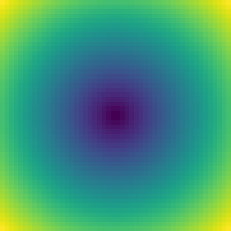
\includegraphics[interpolate=true,width=2.310000in,height=2.310000in]{comp_3d-img0.png}}%
\end{pgfscope}%
\begin{pgfscope}%
\pgfsetbuttcap%
\pgfsetroundjoin%
\definecolor{currentfill}{rgb}{0.000000,0.000000,0.000000}%
\pgfsetfillcolor{currentfill}%
\pgfsetlinewidth{0.803000pt}%
\definecolor{currentstroke}{rgb}{0.000000,0.000000,0.000000}%
\pgfsetstrokecolor{currentstroke}%
\pgfsetdash{}{0pt}%
\pgfsys@defobject{currentmarker}{\pgfqpoint{0.000000in}{-0.048611in}}{\pgfqpoint{0.000000in}{0.000000in}}{%
\pgfpathmoveto{\pgfqpoint{0.000000in}{0.000000in}}%
\pgfpathlineto{\pgfqpoint{0.000000in}{-0.048611in}}%
\pgfusepath{stroke,fill}%
}%
\begin{pgfscope}%
\pgfsys@transformshift{4.085682in}{0.548486in}%
\pgfsys@useobject{currentmarker}{}%
\end{pgfscope}%
\end{pgfscope}%
\begin{pgfscope}%
\definecolor{textcolor}{rgb}{0.000000,0.000000,0.000000}%
\pgfsetstrokecolor{textcolor}%
\pgfsetfillcolor{textcolor}%
\pgftext[x=4.085682in,y=0.451264in,,top]{\color{textcolor}{\rmfamily\fontsize{10.000000}{12.000000}\selectfont\catcode`\^=\active\def^{\ifmmode\sp\else\^{}\fi}\catcode`\%=\active\def%{\%}\ensuremath{-}2}}%
\end{pgfscope}%
\begin{pgfscope}%
\pgfsetbuttcap%
\pgfsetroundjoin%
\definecolor{currentfill}{rgb}{0.000000,0.000000,0.000000}%
\pgfsetfillcolor{currentfill}%
\pgfsetlinewidth{0.803000pt}%
\definecolor{currentstroke}{rgb}{0.000000,0.000000,0.000000}%
\pgfsetstrokecolor{currentstroke}%
\pgfsetdash{}{0pt}%
\pgfsys@defobject{currentmarker}{\pgfqpoint{0.000000in}{-0.048611in}}{\pgfqpoint{0.000000in}{0.000000in}}{%
\pgfpathmoveto{\pgfqpoint{0.000000in}{0.000000in}}%
\pgfpathlineto{\pgfqpoint{0.000000in}{-0.048611in}}%
\pgfusepath{stroke,fill}%
}%
\begin{pgfscope}%
\pgfsys@transformshift{4.855682in}{0.548486in}%
\pgfsys@useobject{currentmarker}{}%
\end{pgfscope}%
\end{pgfscope}%
\begin{pgfscope}%
\definecolor{textcolor}{rgb}{0.000000,0.000000,0.000000}%
\pgfsetstrokecolor{textcolor}%
\pgfsetfillcolor{textcolor}%
\pgftext[x=4.855682in,y=0.451264in,,top]{\color{textcolor}{\rmfamily\fontsize{10.000000}{12.000000}\selectfont\catcode`\^=\active\def^{\ifmmode\sp\else\^{}\fi}\catcode`\%=\active\def%{\%}0}}%
\end{pgfscope}%
\begin{pgfscope}%
\pgfsetbuttcap%
\pgfsetroundjoin%
\definecolor{currentfill}{rgb}{0.000000,0.000000,0.000000}%
\pgfsetfillcolor{currentfill}%
\pgfsetlinewidth{0.803000pt}%
\definecolor{currentstroke}{rgb}{0.000000,0.000000,0.000000}%
\pgfsetstrokecolor{currentstroke}%
\pgfsetdash{}{0pt}%
\pgfsys@defobject{currentmarker}{\pgfqpoint{0.000000in}{-0.048611in}}{\pgfqpoint{0.000000in}{0.000000in}}{%
\pgfpathmoveto{\pgfqpoint{0.000000in}{0.000000in}}%
\pgfpathlineto{\pgfqpoint{0.000000in}{-0.048611in}}%
\pgfusepath{stroke,fill}%
}%
\begin{pgfscope}%
\pgfsys@transformshift{5.625682in}{0.548486in}%
\pgfsys@useobject{currentmarker}{}%
\end{pgfscope}%
\end{pgfscope}%
\begin{pgfscope}%
\definecolor{textcolor}{rgb}{0.000000,0.000000,0.000000}%
\pgfsetstrokecolor{textcolor}%
\pgfsetfillcolor{textcolor}%
\pgftext[x=5.625682in,y=0.451264in,,top]{\color{textcolor}{\rmfamily\fontsize{10.000000}{12.000000}\selectfont\catcode`\^=\active\def^{\ifmmode\sp\else\^{}\fi}\catcode`\%=\active\def%{\%}2}}%
\end{pgfscope}%
\begin{pgfscope}%
\definecolor{textcolor}{rgb}{0.000000,0.000000,0.000000}%
\pgfsetstrokecolor{textcolor}%
\pgfsetfillcolor{textcolor}%
\pgftext[x=4.855682in,y=0.261295in,,top]{\color{textcolor}{\rmfamily\fontsize{12.000000}{14.400000}\selectfont\catcode`\^=\active\def^{\ifmmode\sp\else\^{}\fi}\catcode`\%=\active\def%{\%}$\Re$}}%
\end{pgfscope}%
\begin{pgfscope}%
\pgfsetbuttcap%
\pgfsetroundjoin%
\definecolor{currentfill}{rgb}{0.000000,0.000000,0.000000}%
\pgfsetfillcolor{currentfill}%
\pgfsetlinewidth{0.803000pt}%
\definecolor{currentstroke}{rgb}{0.000000,0.000000,0.000000}%
\pgfsetstrokecolor{currentstroke}%
\pgfsetdash{}{0pt}%
\pgfsys@defobject{currentmarker}{\pgfqpoint{-0.048611in}{0.000000in}}{\pgfqpoint{-0.000000in}{0.000000in}}{%
\pgfpathmoveto{\pgfqpoint{-0.000000in}{0.000000in}}%
\pgfpathlineto{\pgfqpoint{-0.048611in}{0.000000in}}%
\pgfusepath{stroke,fill}%
}%
\begin{pgfscope}%
\pgfsys@transformshift{3.700682in}{0.548486in}%
\pgfsys@useobject{currentmarker}{}%
\end{pgfscope}%
\end{pgfscope}%
\begin{pgfscope}%
\definecolor{textcolor}{rgb}{0.000000,0.000000,0.000000}%
\pgfsetstrokecolor{textcolor}%
\pgfsetfillcolor{textcolor}%
\pgftext[x=3.407069in, y=0.495724in, left, base]{\color{textcolor}{\rmfamily\fontsize{10.000000}{12.000000}\selectfont\catcode`\^=\active\def^{\ifmmode\sp\else\^{}\fi}\catcode`\%=\active\def%{\%}\ensuremath{-}3}}%
\end{pgfscope}%
\begin{pgfscope}%
\pgfsetbuttcap%
\pgfsetroundjoin%
\definecolor{currentfill}{rgb}{0.000000,0.000000,0.000000}%
\pgfsetfillcolor{currentfill}%
\pgfsetlinewidth{0.803000pt}%
\definecolor{currentstroke}{rgb}{0.000000,0.000000,0.000000}%
\pgfsetstrokecolor{currentstroke}%
\pgfsetdash{}{0pt}%
\pgfsys@defobject{currentmarker}{\pgfqpoint{-0.048611in}{0.000000in}}{\pgfqpoint{-0.000000in}{0.000000in}}{%
\pgfpathmoveto{\pgfqpoint{-0.000000in}{0.000000in}}%
\pgfpathlineto{\pgfqpoint{-0.048611in}{0.000000in}}%
\pgfusepath{stroke,fill}%
}%
\begin{pgfscope}%
\pgfsys@transformshift{3.700682in}{0.933486in}%
\pgfsys@useobject{currentmarker}{}%
\end{pgfscope}%
\end{pgfscope}%
\begin{pgfscope}%
\definecolor{textcolor}{rgb}{0.000000,0.000000,0.000000}%
\pgfsetstrokecolor{textcolor}%
\pgfsetfillcolor{textcolor}%
\pgftext[x=3.407069in, y=0.880724in, left, base]{\color{textcolor}{\rmfamily\fontsize{10.000000}{12.000000}\selectfont\catcode`\^=\active\def^{\ifmmode\sp\else\^{}\fi}\catcode`\%=\active\def%{\%}\ensuremath{-}2}}%
\end{pgfscope}%
\begin{pgfscope}%
\pgfsetbuttcap%
\pgfsetroundjoin%
\definecolor{currentfill}{rgb}{0.000000,0.000000,0.000000}%
\pgfsetfillcolor{currentfill}%
\pgfsetlinewidth{0.803000pt}%
\definecolor{currentstroke}{rgb}{0.000000,0.000000,0.000000}%
\pgfsetstrokecolor{currentstroke}%
\pgfsetdash{}{0pt}%
\pgfsys@defobject{currentmarker}{\pgfqpoint{-0.048611in}{0.000000in}}{\pgfqpoint{-0.000000in}{0.000000in}}{%
\pgfpathmoveto{\pgfqpoint{-0.000000in}{0.000000in}}%
\pgfpathlineto{\pgfqpoint{-0.048611in}{0.000000in}}%
\pgfusepath{stroke,fill}%
}%
\begin{pgfscope}%
\pgfsys@transformshift{3.700682in}{1.318486in}%
\pgfsys@useobject{currentmarker}{}%
\end{pgfscope}%
\end{pgfscope}%
\begin{pgfscope}%
\definecolor{textcolor}{rgb}{0.000000,0.000000,0.000000}%
\pgfsetstrokecolor{textcolor}%
\pgfsetfillcolor{textcolor}%
\pgftext[x=3.407069in, y=1.265724in, left, base]{\color{textcolor}{\rmfamily\fontsize{10.000000}{12.000000}\selectfont\catcode`\^=\active\def^{\ifmmode\sp\else\^{}\fi}\catcode`\%=\active\def%{\%}\ensuremath{-}1}}%
\end{pgfscope}%
\begin{pgfscope}%
\pgfsetbuttcap%
\pgfsetroundjoin%
\definecolor{currentfill}{rgb}{0.000000,0.000000,0.000000}%
\pgfsetfillcolor{currentfill}%
\pgfsetlinewidth{0.803000pt}%
\definecolor{currentstroke}{rgb}{0.000000,0.000000,0.000000}%
\pgfsetstrokecolor{currentstroke}%
\pgfsetdash{}{0pt}%
\pgfsys@defobject{currentmarker}{\pgfqpoint{-0.048611in}{0.000000in}}{\pgfqpoint{-0.000000in}{0.000000in}}{%
\pgfpathmoveto{\pgfqpoint{-0.000000in}{0.000000in}}%
\pgfpathlineto{\pgfqpoint{-0.048611in}{0.000000in}}%
\pgfusepath{stroke,fill}%
}%
\begin{pgfscope}%
\pgfsys@transformshift{3.700682in}{1.703486in}%
\pgfsys@useobject{currentmarker}{}%
\end{pgfscope}%
\end{pgfscope}%
\begin{pgfscope}%
\definecolor{textcolor}{rgb}{0.000000,0.000000,0.000000}%
\pgfsetstrokecolor{textcolor}%
\pgfsetfillcolor{textcolor}%
\pgftext[x=3.515094in, y=1.650724in, left, base]{\color{textcolor}{\rmfamily\fontsize{10.000000}{12.000000}\selectfont\catcode`\^=\active\def^{\ifmmode\sp\else\^{}\fi}\catcode`\%=\active\def%{\%}0}}%
\end{pgfscope}%
\begin{pgfscope}%
\pgfsetbuttcap%
\pgfsetroundjoin%
\definecolor{currentfill}{rgb}{0.000000,0.000000,0.000000}%
\pgfsetfillcolor{currentfill}%
\pgfsetlinewidth{0.803000pt}%
\definecolor{currentstroke}{rgb}{0.000000,0.000000,0.000000}%
\pgfsetstrokecolor{currentstroke}%
\pgfsetdash{}{0pt}%
\pgfsys@defobject{currentmarker}{\pgfqpoint{-0.048611in}{0.000000in}}{\pgfqpoint{-0.000000in}{0.000000in}}{%
\pgfpathmoveto{\pgfqpoint{-0.000000in}{0.000000in}}%
\pgfpathlineto{\pgfqpoint{-0.048611in}{0.000000in}}%
\pgfusepath{stroke,fill}%
}%
\begin{pgfscope}%
\pgfsys@transformshift{3.700682in}{2.088486in}%
\pgfsys@useobject{currentmarker}{}%
\end{pgfscope}%
\end{pgfscope}%
\begin{pgfscope}%
\definecolor{textcolor}{rgb}{0.000000,0.000000,0.000000}%
\pgfsetstrokecolor{textcolor}%
\pgfsetfillcolor{textcolor}%
\pgftext[x=3.515094in, y=2.035724in, left, base]{\color{textcolor}{\rmfamily\fontsize{10.000000}{12.000000}\selectfont\catcode`\^=\active\def^{\ifmmode\sp\else\^{}\fi}\catcode`\%=\active\def%{\%}1}}%
\end{pgfscope}%
\begin{pgfscope}%
\pgfsetbuttcap%
\pgfsetroundjoin%
\definecolor{currentfill}{rgb}{0.000000,0.000000,0.000000}%
\pgfsetfillcolor{currentfill}%
\pgfsetlinewidth{0.803000pt}%
\definecolor{currentstroke}{rgb}{0.000000,0.000000,0.000000}%
\pgfsetstrokecolor{currentstroke}%
\pgfsetdash{}{0pt}%
\pgfsys@defobject{currentmarker}{\pgfqpoint{-0.048611in}{0.000000in}}{\pgfqpoint{-0.000000in}{0.000000in}}{%
\pgfpathmoveto{\pgfqpoint{-0.000000in}{0.000000in}}%
\pgfpathlineto{\pgfqpoint{-0.048611in}{0.000000in}}%
\pgfusepath{stroke,fill}%
}%
\begin{pgfscope}%
\pgfsys@transformshift{3.700682in}{2.473486in}%
\pgfsys@useobject{currentmarker}{}%
\end{pgfscope}%
\end{pgfscope}%
\begin{pgfscope}%
\definecolor{textcolor}{rgb}{0.000000,0.000000,0.000000}%
\pgfsetstrokecolor{textcolor}%
\pgfsetfillcolor{textcolor}%
\pgftext[x=3.515094in, y=2.420724in, left, base]{\color{textcolor}{\rmfamily\fontsize{10.000000}{12.000000}\selectfont\catcode`\^=\active\def^{\ifmmode\sp\else\^{}\fi}\catcode`\%=\active\def%{\%}2}}%
\end{pgfscope}%
\begin{pgfscope}%
\pgfsetbuttcap%
\pgfsetroundjoin%
\definecolor{currentfill}{rgb}{0.000000,0.000000,0.000000}%
\pgfsetfillcolor{currentfill}%
\pgfsetlinewidth{0.803000pt}%
\definecolor{currentstroke}{rgb}{0.000000,0.000000,0.000000}%
\pgfsetstrokecolor{currentstroke}%
\pgfsetdash{}{0pt}%
\pgfsys@defobject{currentmarker}{\pgfqpoint{-0.048611in}{0.000000in}}{\pgfqpoint{-0.000000in}{0.000000in}}{%
\pgfpathmoveto{\pgfqpoint{-0.000000in}{0.000000in}}%
\pgfpathlineto{\pgfqpoint{-0.048611in}{0.000000in}}%
\pgfusepath{stroke,fill}%
}%
\begin{pgfscope}%
\pgfsys@transformshift{3.700682in}{2.858486in}%
\pgfsys@useobject{currentmarker}{}%
\end{pgfscope}%
\end{pgfscope}%
\begin{pgfscope}%
\definecolor{textcolor}{rgb}{0.000000,0.000000,0.000000}%
\pgfsetstrokecolor{textcolor}%
\pgfsetfillcolor{textcolor}%
\pgftext[x=3.515094in, y=2.805724in, left, base]{\color{textcolor}{\rmfamily\fontsize{10.000000}{12.000000}\selectfont\catcode`\^=\active\def^{\ifmmode\sp\else\^{}\fi}\catcode`\%=\active\def%{\%}3}}%
\end{pgfscope}%
\begin{pgfscope}%
\definecolor{textcolor}{rgb}{0.000000,0.000000,0.000000}%
\pgfsetstrokecolor{textcolor}%
\pgfsetfillcolor{textcolor}%
\pgftext[x=3.351514in,y=1.703486in,,bottom,rotate=90.000000]{\color{textcolor}{\rmfamily\fontsize{12.000000}{14.400000}\selectfont\catcode`\^=\active\def^{\ifmmode\sp\else\^{}\fi}\catcode`\%=\active\def%{\%}$\Im$}}%
\end{pgfscope}%
\begin{pgfscope}%
\pgfpathrectangle{\pgfqpoint{3.700682in}{0.548486in}}{\pgfqpoint{2.310000in}{2.310000in}}%
\pgfusepath{clip}%
\pgfsetrectcap%
\pgfsetroundjoin%
\pgfsetlinewidth{1.505625pt}%
\definecolor{currentstroke}{rgb}{0.000000,0.000000,0.000000}%
\pgfsetstrokecolor{currentstroke}%
\pgfsetdash{}{0pt}%
\pgfpathmoveto{\pgfqpoint{3.700682in}{1.703486in}}%
\pgfpathlineto{\pgfqpoint{6.010682in}{1.703486in}}%
\pgfusepath{stroke}%
\end{pgfscope}%
\begin{pgfscope}%
\pgfpathrectangle{\pgfqpoint{3.700682in}{0.548486in}}{\pgfqpoint{2.310000in}{2.310000in}}%
\pgfusepath{clip}%
\pgfsetrectcap%
\pgfsetroundjoin%
\pgfsetlinewidth{1.505625pt}%
\definecolor{currentstroke}{rgb}{0.000000,0.000000,0.000000}%
\pgfsetstrokecolor{currentstroke}%
\pgfsetdash{}{0pt}%
\pgfpathmoveto{\pgfqpoint{4.855682in}{0.548486in}}%
\pgfpathlineto{\pgfqpoint{4.855682in}{2.858486in}}%
\pgfusepath{stroke}%
\end{pgfscope}%
\begin{pgfscope}%
\pgfsetbuttcap%
\pgfsetmiterjoin%
\definecolor{currentfill}{rgb}{1.000000,1.000000,1.000000}%
\pgfsetfillcolor{currentfill}%
\pgfsetlinewidth{0.000000pt}%
\definecolor{currentstroke}{rgb}{0.000000,0.000000,0.000000}%
\pgfsetstrokecolor{currentstroke}%
\pgfsetstrokeopacity{0.000000}%
\pgfsetdash{}{0pt}%
\pgfpathmoveto{\pgfqpoint{6.169205in}{0.548486in}}%
\pgfpathlineto{\pgfqpoint{6.284705in}{0.548486in}}%
\pgfpathlineto{\pgfqpoint{6.284705in}{2.858486in}}%
\pgfpathlineto{\pgfqpoint{6.169205in}{2.858486in}}%
\pgfpathlineto{\pgfqpoint{6.169205in}{0.548486in}}%
\pgfpathclose%
\pgfusepath{fill}%
\end{pgfscope}%
\begin{pgfscope}%
\pgfsys@transformshift{6.170000in}{0.551248in}%
\pgftext[left,bottom]{
\includegraphics[interpolate=true,width=0.110000in,height=2.310000in]{comp_3d-img1.png}}%
\end{pgfscope}%
\begin{pgfscope}%
\pgfsetbuttcap%
\pgfsetroundjoin%
\definecolor{currentfill}{rgb}{0.000000,0.000000,0.000000}%
\pgfsetfillcolor{currentfill}%
\pgfsetlinewidth{0.803000pt}%
\definecolor{currentstroke}{rgb}{0.000000,0.000000,0.000000}%
\pgfsetstrokecolor{currentstroke}%
\pgfsetdash{}{0pt}%
\pgfsys@defobject{currentmarker}{\pgfqpoint{0.000000in}{0.000000in}}{\pgfqpoint{0.048611in}{0.000000in}}{%
\pgfpathmoveto{\pgfqpoint{0.000000in}{0.000000in}}%
\pgfpathlineto{\pgfqpoint{0.048611in}{0.000000in}}%
\pgfusepath{stroke,fill}%
}%
\begin{pgfscope}%
\pgfsys@transformshift{6.284705in}{1.056176in}%
\pgfsys@useobject{currentmarker}{}%
\end{pgfscope}%
\end{pgfscope}%
\begin{pgfscope}%
\definecolor{textcolor}{rgb}{0.000000,0.000000,0.000000}%
\pgfsetstrokecolor{textcolor}%
\pgfsetfillcolor{textcolor}%
\pgftext[x=6.381927in, y=1.003415in, left, base]{\color{textcolor}{\rmfamily\fontsize{10.000000}{12.000000}\selectfont\catcode`\^=\active\def^{\ifmmode\sp\else\^{}\fi}\catcode`\%=\active\def%{\%}1}}%
\end{pgfscope}%
\begin{pgfscope}%
\pgfsetbuttcap%
\pgfsetroundjoin%
\definecolor{currentfill}{rgb}{0.000000,0.000000,0.000000}%
\pgfsetfillcolor{currentfill}%
\pgfsetlinewidth{0.803000pt}%
\definecolor{currentstroke}{rgb}{0.000000,0.000000,0.000000}%
\pgfsetstrokecolor{currentstroke}%
\pgfsetdash{}{0pt}%
\pgfsys@defobject{currentmarker}{\pgfqpoint{0.000000in}{0.000000in}}{\pgfqpoint{0.048611in}{0.000000in}}{%
\pgfpathmoveto{\pgfqpoint{0.000000in}{0.000000in}}%
\pgfpathlineto{\pgfqpoint{0.048611in}{0.000000in}}%
\pgfusepath{stroke,fill}%
}%
\begin{pgfscope}%
\pgfsys@transformshift{6.284705in}{1.611992in}%
\pgfsys@useobject{currentmarker}{}%
\end{pgfscope}%
\end{pgfscope}%
\begin{pgfscope}%
\definecolor{textcolor}{rgb}{0.000000,0.000000,0.000000}%
\pgfsetstrokecolor{textcolor}%
\pgfsetfillcolor{textcolor}%
\pgftext[x=6.381927in, y=1.559230in, left, base]{\color{textcolor}{\rmfamily\fontsize{10.000000}{12.000000}\selectfont\catcode`\^=\active\def^{\ifmmode\sp\else\^{}\fi}\catcode`\%=\active\def%{\%}2}}%
\end{pgfscope}%
\begin{pgfscope}%
\pgfsetbuttcap%
\pgfsetroundjoin%
\definecolor{currentfill}{rgb}{0.000000,0.000000,0.000000}%
\pgfsetfillcolor{currentfill}%
\pgfsetlinewidth{0.803000pt}%
\definecolor{currentstroke}{rgb}{0.000000,0.000000,0.000000}%
\pgfsetstrokecolor{currentstroke}%
\pgfsetdash{}{0pt}%
\pgfsys@defobject{currentmarker}{\pgfqpoint{0.000000in}{0.000000in}}{\pgfqpoint{0.048611in}{0.000000in}}{%
\pgfpathmoveto{\pgfqpoint{0.000000in}{0.000000in}}%
\pgfpathlineto{\pgfqpoint{0.048611in}{0.000000in}}%
\pgfusepath{stroke,fill}%
}%
\begin{pgfscope}%
\pgfsys@transformshift{6.284705in}{2.167807in}%
\pgfsys@useobject{currentmarker}{}%
\end{pgfscope}%
\end{pgfscope}%
\begin{pgfscope}%
\definecolor{textcolor}{rgb}{0.000000,0.000000,0.000000}%
\pgfsetstrokecolor{textcolor}%
\pgfsetfillcolor{textcolor}%
\pgftext[x=6.381927in, y=2.115046in, left, base]{\color{textcolor}{\rmfamily\fontsize{10.000000}{12.000000}\selectfont\catcode`\^=\active\def^{\ifmmode\sp\else\^{}\fi}\catcode`\%=\active\def%{\%}3}}%
\end{pgfscope}%
\begin{pgfscope}%
\pgfsetbuttcap%
\pgfsetroundjoin%
\definecolor{currentfill}{rgb}{0.000000,0.000000,0.000000}%
\pgfsetfillcolor{currentfill}%
\pgfsetlinewidth{0.803000pt}%
\definecolor{currentstroke}{rgb}{0.000000,0.000000,0.000000}%
\pgfsetstrokecolor{currentstroke}%
\pgfsetdash{}{0pt}%
\pgfsys@defobject{currentmarker}{\pgfqpoint{0.000000in}{0.000000in}}{\pgfqpoint{0.048611in}{0.000000in}}{%
\pgfpathmoveto{\pgfqpoint{0.000000in}{0.000000in}}%
\pgfpathlineto{\pgfqpoint{0.048611in}{0.000000in}}%
\pgfusepath{stroke,fill}%
}%
\begin{pgfscope}%
\pgfsys@transformshift{6.284705in}{2.723623in}%
\pgfsys@useobject{currentmarker}{}%
\end{pgfscope}%
\end{pgfscope}%
\begin{pgfscope}%
\definecolor{textcolor}{rgb}{0.000000,0.000000,0.000000}%
\pgfsetstrokecolor{textcolor}%
\pgfsetfillcolor{textcolor}%
\pgftext[x=6.381927in, y=2.670861in, left, base]{\color{textcolor}{\rmfamily\fontsize{10.000000}{12.000000}\selectfont\catcode`\^=\active\def^{\ifmmode\sp\else\^{}\fi}\catcode`\%=\active\def%{\%}4}}%
\end{pgfscope}%
\begin{pgfscope}%
\pgfsetrectcap%
\pgfsetmiterjoin%
\pgfsetlinewidth{0.803000pt}%
\definecolor{currentstroke}{rgb}{0.000000,0.000000,0.000000}%
\pgfsetstrokecolor{currentstroke}%
\pgfsetdash{}{0pt}%
\pgfpathmoveto{\pgfqpoint{6.169205in}{0.548486in}}%
\pgfpathlineto{\pgfqpoint{6.226955in}{0.548486in}}%
\pgfpathlineto{\pgfqpoint{6.284705in}{0.548486in}}%
\pgfpathlineto{\pgfqpoint{6.284705in}{2.858486in}}%
\pgfpathlineto{\pgfqpoint{6.226955in}{2.858486in}}%
\pgfpathlineto{\pgfqpoint{6.169205in}{2.858486in}}%
\pgfpathlineto{\pgfqpoint{6.169205in}{0.548486in}}%
\pgfpathclose%
\pgfusepath{stroke}%
\end{pgfscope}%
\end{pgfpicture}%
\makeatother%
\endgroup%

	\caption{Zwei Arten den Betrag einer Komplexen Zahl zu plotten.}
	\label{fig:komp_3D}
\end{figure}


\section{Komplexe Zahlen in Python}

In \texttt{Python} wird die Zahl $i$ durch \texttt{1j} ausgedrückt. \texttt{j} alleine hat zunächst keine Bedeutung und führt zu einer Fehlermeldung wenn \texttt{j} nicht definiert ist. \texttt{1j} hingegen ist $1\cdot i$, wobei \texttt{1} hier durch andere zahlen ersetzt werden kann, zB \texttt{5j} ($=5\cdot i$) oder \texttt{2.7j}($=2.7 \cdot i$). Die folgende (ein wenig gekürzte) Aufzeichnung einer interaktiven \texttt{iPython} Session soll diesen vielleicht im ersten Moment verwirrenden Unterschied klar machen:

\begin{python}{Verwendung von i in Python.}
In [1]: %pylab

In [2]: 1j
Out[2]: 1j

In [3]: j

NameError: name 'j' is not defined

In [4]: b = 3

In [5]: 2 + bj

NameError: name 'bj' is not defined

In [6]: 2 + b*1j
Out[6]: (2+3j)
\end{python}



\begin{table}[H]
    \centering
    \begin{tabular}{|p{3cm}|p{6cm}|p{6cm}|}
        \hline
    \textbf{Befehl} & \textbf{Beispiel} & \textbf{Kommentar} \\ \hline
    
    \texttt{1j} & \texttt{z = 3+5j} & Die Zahl $i$. \\ \hline
    \texttt{abs()} & \texttt{r = abs(z)} & Berechnet den Betrag von \texttt{z}. \\ \hline
    \texttt{angle()} & \texttt{phi = angle(z)} & Berechnet das Argument von \texttt{z}. \\ \hline


    \end{tabular}
\end{table}




\todo[inline]{ polynome mit reellen koeefizienten -> kompl konj oder reelle nullstellen. Division von compl zahlen durch mult mit kompl. konj., $e^z$, $ln z$, python, 3d plots of complex functions}

\section{Anwendungen}\label{sec:anwendungen}
\todo[]{TODO}

\section{Aufgaben}
\todo[]{TODO}


